\documentclass[]{book}
%PACKAGE LOADING
\usepackage{etex}
\usepackage{fancyvrb}
\usepackage{booktabs}
\usepackage{graphics}
\renewcommand{\arraystretch}{1.2}
\usepackage[section]{placeins}
%\usepackage[md]{titlesec}
\usepackage{makeidx}
\usepackage{mathpazo}
\usepackage{mathptmx}
\usepackage{nameref}
\usepackage{xspace}
\usepackage{comment}
\usepackage{tikz}
\usepackage{tikz-qtree}
\usepackage{multicol}
%\usepackage{tocloft}
%Make tocloft and titlesec play nicely together
%\makeatletter
%\AtBeginDocument{
%   \renewcommand\@cftmaketoctitle{\chapter*{\contentsname}}
%}
%\makeatother

\renewcommand{\rmdefault}{ppl} % rm
%\usepackage{palatino}
\usepackage[scaled=0.9]{beramono}
\usepackage[T1]{fontenc}
%\usepackage[protrusion=true,expansion=true]{microtype}
\usepackage[left=3cm, right=1.5cm, top=2cm, bottom=1.8cm, paperwidth=7.5in, paperheight=9.25in]{geometry}
\usepackage{upquote}
\usepackage{mathtools}
\usepackage[draft=false]{hyperref}
\usepackage{fancyhdr}
\usepackage{emptypage}
\usepackage{underscore}
\usepackage{upquote,textcomp}
\newcommand\upquote[1]{\textquotesingle#1\textquotesingle}

\pagestyle{fancy}
\fancyhead[lo]{\slshape\nouppercase{\leftmark}\hfill\thepage}
\fancyhead[re]{\thepage\hfill\slshape\nouppercase{\leftmark}}
\fancyfoot{}
%\fancyfoot[LE,RO]{\thepage}
\renewcommand{\headrulewidth}{0pt}
\renewcommand{\footrulewidth}{0pt}

%Table of contents spacing
%\setlength\cftparskip{5pt}
%\setlength\cftbeforechapskip{0pt}

\usepackage[columns=3]{idxlayout}
\makeindex

%OUR MACROS FOR THIS BOOK

%The starting off interludes

\newcommand{\sofarstartingoff}{

\noindent 1

\noindent Integers \texttt{min\_int} \ldots\ \texttt{-3}\ \texttt{-2}\ \texttt{-1}\ \texttt{0}\ \texttt{1}\ \texttt{2}\ \texttt{3}\ \ldots\ \texttt{max\_int} of type \textbf{\textrm{int}}. Booleans \texttt{true} and \texttt{false} of type \textbf{\textrm{bool}}. \noindent Characters of type \textrm{\textbf{char}} like \texttt{\upquote{X}} and \texttt{\upquote{!}}. Mathematical operators \texttt{+} \texttt{-} \texttt{*} \texttt{/} \texttt{mod} which take two integers and give another. Operators \texttt{=} \texttt{<} \texttt{<=} \texttt{>} \texttt{>=} \texttt{<>} which compare two values and evaluate to either \texttt{true} or \texttt{false}. The conditional \textbf{\texttt{if}} \textit{expression1} \textbf{\texttt{then}} \textit{expression2} \textbf{\texttt{else}} \textit{expression3}, where \textit{expresssion1} has type \textrm{\textbf{bool}} and \textit{expression2} and \textit{expression3} have the same type as one another. The boolean operators \texttt{\&\&} and \texttt{||} which allow us to build compound boolean expressions.}

\newcommand{\sofarfunctions}
{
\noindent 2

\noindent Assigning a name to the result of evaluating an expression using the \textbf{\texttt{let}}\ \textit{name} \texttt{=}\ \textit{expression} construct. Building compound expressions using \textbf{\texttt{let}}\ \textit{name1} \texttt{=} \textit{expression1} \textbf{\texttt{in}}\ \textbf{\texttt{let}}\ \textit{name2} \texttt{=}\ \textit{expression2} \textbf{\texttt{in}}\ \ldots \ Functions, introduced by \textbf{\texttt{let}}\ \textit{name} \textit{argument1} \textit{argument2} \ldots\ \texttt{=}\ \textit{expression}. These have type $\alpha \rightarrow \beta$, $\alpha \rightarrow \beta \rightarrow \gamma$ etc. for some types $\alpha$, $\beta$, $\gamma$ etc. Recursive functions, which are introduced in the same way, but using \textbf{\texttt{let rec}} instead of \textbf{\texttt{let}}.}

\newcommand{\sofarcasebycase}
{\noindent 3

\noindent Matching patterns using \textbf{\texttt{match}} \textit{expression1} \textbf{\texttt{with}} \textit{pattern1} \texttt{|} \ldots\ \texttt{->} \textit{expression2} \texttt{|} \textit{pattern2} \texttt{|} \ldots\ \texttt{->} \textit{expression3} \texttt{|}\ldots \ The expressions \textit{expression2}, \textit{expression3} etc. must have the same type as one another, and this is the type of the whole \textbf{\texttt{match} \ldots\ \texttt{with}} expression.}

\newcommand{\sofarlistingthings}
{
\noindent 4

\noindent Lists, which are ordered collections of zero or more elements of like type. They are written between square brackets, with elements separated by semicolons e.g. \texttt{[1;\! 2;\! 3;\! 4;\! 5]}. If a list is non-empty, it has a head, which is its first element, and a tail, which is the list composed of the rest of the elements. The \texttt{::}\ ``cons'' operator, which adds an element to the front of a list. The \texttt{@} ``append'' operator, which concatenates two lists together. Lists and the \texttt{::}\ ``cons'' symbol may be used for pattern matching to distinguish lists of length zero, one, etc. and with particular contents.}

\newcommand{\sofarsortingthings}
{
\noindent 5

\noindent Matching two or more things at once, using commas to separate as in \texttt{\textbf{match}} \texttt{a, b} \textbf{\texttt{with}} \texttt{0, 0 ->} \textit{expression1} \texttt{|\ x, y ->} \textit{expression2} \texttt{|} \ldots
}

\newcommand{\sofarfunctionsuponfunctions}
{
\noindent 6

\noindent Anonymous functions \textbf{\texttt{fun}} \textit{name} \texttt{->} \textit{expression}. Making operators into functions as in \texttt{(\! <\! )} and \texttt{(\! +\! )}.
}

\newcommand{\sofarwhenthingsgowrong}
{
\noindent 7

\noindent Defining exceptions with \textbf{\texttt{exception}} \textit{name}. They can carry extra information by adding \textbf{\texttt{of}} \textit{type}. Raising exceptions with \textbf{\texttt{raise}}. Handling exceptions with \textbf{\texttt{try}} \ldots\ \textbf{\texttt{with}}\ \ldots}

\newcommand{\sofarlookingthingsup}
{
\noindent 8

\noindent Tuples to combine a fixed number of elements \texttt{(a,\! b)},\!    \ \texttt{(a,\! b,\! c)} etc. with types \textrm{\textbf{$\alpha$ $\times$ $\beta$}},\ \  \textrm{\textbf{$\alpha$ $\times$ $\beta$ $\times$ $\gamma$}} etc.
}

\newcommand{\sofarmorewithfunctions}
{
\noindent 9

\noindent Partial application of functions by giving fewer than the full number of arguments. Partial application with functions built from operators.
}

\newcommand{\sofarnewkindsofdata}
{
\noindent 10

\noindent New types with \textbf{\texttt{type}} \textit{name} \texttt{=} \textit{constructor1} \textbf{\texttt{of}} \textit{type1} \texttt{|} \textit{constructor2} \textbf{\texttt{of}} \textit{type2} \texttt{|} \ldots\ Pattern matching on them as with the built-in types. Polymorphic types.
}

\newcommand{\sofargrowingtrees}
{
\noindent 11

\noindent Strings, which are sequences of characters written between double quotes and are of type \textbf{\textrm{string}}.
}

\newcommand{\sofarinandout}
{
\noindent 12

\noindent The value \texttt{()} and its type \textbf{\textrm{unit}}. Input channels of type \textrm{\textbf{in\raisebox{1.5pt}{\_}channel}} and output channels of type \textrm{\textbf{out\raisebox{1.5pt}{\_}channel}}. Built-in functions for reading from and writing to them respectively.
}

\newcommand{\sofarputtingthingsinboxes}
{
\noindent 13

\noindent References of type \textrm{\textbf{$\alpha$ ref}}. Building them using  \texttt{ref}, accessing their contents using \texttt{!} and updating them using the \texttt{:=}\, operator. Bracketing expressions together with \textbf{\texttt{begin}} and \textbf{\texttt{end}} instead of parentheses for readability. Performing an action many times based on a boolean condition with the \textbf{\texttt{while}} \textit{boolean expression} \texttt{\textbf{do}}  \textit{expression} \texttt{\textbf{done}} construct. Performing an action a fixed number of times with a varying parameter using the \textbf{\texttt{for}} \textit{name} \texttt{=} \textit{start} \texttt{\textbf{to}}  \textit{end} \texttt{\textbf{do}} \textit{expression} \texttt{\textbf{done}} construct. Arrays of type \textrm{\textbf{$\alpha$ array}}. Creating an array with the built-in function \texttt{Array.make}, finding its length with \texttt{Array.length}, accessing an element with \texttt{a.(}\textit{subscript}\texttt{)}. Updating with \texttt{a.(}\textit{subscript}\texttt{) <-} \textit{expression}. The built-in function \texttt{String.iter}.

}

\newcommand{\sofargettingreal}
{
\noindent 14

\noindent Floating-point numbers \texttt{min\_float} \ldots\ \texttt{max\_float} of type \textrm{\textbf{float}}. \noindent Floating-point operators \texttt{+.} \texttt{*.} \texttt{-.} \texttt{/.} \texttt{**} and built-in functions \texttt{sqrt} \texttt{log} etc.}

\newcommand{\sofartheocamlstandardlibrary}
{
\noindent 15

\noindent Using functions from the OCaml Standard Library with the form \textit{Module}\texttt{.}\textit{function}.
}

\newcommand{\sofarbuildingbiggerprograms}
{

\noindent 16

\noindent Writing modules in \texttt{.ml} files. Building interfaces in \texttt{.mli} files with types and \textbf{\texttt{val}}. Using the \texttt{ocamlc} and \texttt{ocamlopt} compilers. Comments written between \texttt{(*} and \texttt{*)}.}

% For comparison, the existing overlap macros:
% \def\llap#1{\hbox to 0pt{\hss#1}}
% \def\rlap#1{\hbox to 0pt{#1\hss}}
\def\clap#1{\hbox to 0pt{\hss#1\hss}}
\def\mathllap{\mathpalette\mathllapinternal}
\def\mathrlap{\mathpalette\mathrlapinternal}
\def\mathclap{\mathpalette\mathclapinternal}
\def\mathllapinternal#1#2{%
           \llap{$\mathsurround=0pt#1{#2}$}}
\def\mathrlapinternal#1#2{%
           \rlap{$\mathsurround=0pt#1{#2}$}}
\def\mathclapinternal#1#2{%
           \clap{$\mathsurround=0pt#1{#2}$}}

%Over and under brackets for full type annotations
\newcommand{\obn}[1]{\overbracket[0pt][0pt]{\vphantom{\texttt{0}}#1}}
\newcommand{\ob}[1]{\overbracket[0.5pt][1pt]{\vphantom{\texttt{0}}#1}}
\newcommand{\ubn}[1]{\underbracket[0pt][0pt]{\vphantom{\texttt{0}}#1}}
\newcommand{\ub}[1]{\underbracket[0.5pt][1pt]{\vphantom{\texttt{0}}#1}}

%Single line code fragments, done in math mode with type annotations
\newcommand{\goesto}{\ \rightarrow\ }
\newcommand{\equals}{\texttt{=}}
\newcommand{\varx}{\texttt{x}}
\newcommand{\vary}{\texttt{y}}
\newcommand{\tint}{\textit{int}}
\newcommand{\tbool}{\textit{bool}}
\newcommand{\kif}{\texttt{if}}
\newcommand{\kthen}{\texttt{then}}
\newcommand{\kelse}{\texttt{else}}

%Multiline code fragments, which do not usually have type annotations
\newcommand{\pletrec}{\textbf{let rec}\xspace}
\newcommand{\plet}{\textbf{let}\xspace}
\newcommand{\pin}{\textbf{in}\xspace}
\newcommand{\pmatch}{\textbf{match}\xspace}
\newcommand{\pwith}{\textbf{with}\xspace}
\newcommand{\pif}{\textbf{if}\xspace}
\newcommand{\pfun}{\textbf{fun}\xspace}
\newcommand{\pfunction}{\textbf{function}\xspace}
\newcommand{\pthen}{\textbf{then}\xspace}
\newcommand{\pelse}{\textbf{else}\xspace}
\newcommand{\praise}{\textbf{raise}\xspace}
\newcommand{\ptry}{\textbf{try}\xspace}
\newcommand{\ptype}{\textbf{type}\xspace}
\newcommand{\pof}{\textbf{of}\xspace}
\newcommand{\pand}{\textbf{and}\xspace}
\newcommand{\pexception}{\textbf{exception}\xspace}
\newcommand{\pwhile}{\textbf{while}\xspace}
\newcommand{\pfor}{\textbf{for}\xspace}
\newcommand{\pto}{\textbf{to}\xspace}
\newcommand{\pdo}{\textbf{do}\xspace}
\newcommand{\pdone}{\textbf{done}\xspace}
\newcommand{\pbegin}{\textbf{begin}\xspace}
\newcommand{\pend}{\textbf{end}\xspace}

%\renewcommand{\cftchapfont}{\normalfont}
%\renewcommand{\cftchappagefont}{\normalfont}

\newcommand{\smspace}{\vspace{4mm}}

%BEGINNING OF ACTUAL DOCUMENT
\begin{document}
\frontmatter

%Pre-title verso
\thispagestyle{empty}

{\Large\scshape OCaml from the Very Beginning}

\vspace{16mm}

\begin{minipage}{5in}
\setlength{\parindent}{25pt}
\noindent In \textit{OCaml from the Very Beginning} John Whitington takes a no-prerequisites approach to teaching a modern general-purpose programming language. Each small, self-contained chapter introduces a new topic, building until the reader can write quite substantial programs. There are plenty of questions and, crucially, worked answers and hints.

\textit{OCaml from the Very Beginning} will appeal both to new programmers, and experienced programmers eager to explore functional languages such as OCaml. It is suitable both for formal use within an undergraduate or graduate curriculum, and for the interested amateur.

\vspace{8mm}

\noindent{\hyphenpenalty=10000\begin{sloppypar}\noindent\textsc{John Whitington} founded a software company which uses OCaml extensively. He teaches functional programming to students of Computer Science at the University of Cambridge.\end{sloppypar}}\end{minipage}


\cleardoublepage %recto
\chapter*{} %get pagebreak into kindle

%Title Verso
\thispagestyle{empty}

\begin{center}
\vphantom{a}%to get vspace to work

\vspace{50mm}

{\Huge\scshape OCaml

\textit{\LARGE from the very beginning}

}

\vspace{20mm}

{John Whitington}

\vspace{85mm}

{\scshape C O H E R E N T \ \ P R E S S}
\end{center}

\clearpage

\chapter*{} %get pagebreak into kindle
%Title Recto
\thispagestyle{empty}

\begin{center}

\vphantom{a}%to get vspace to work

\vspace{10mm}

\noindent C O H E R E N T \ \ \ P R E S S\\ \vspace{1mm} \footnotesize Cambridge

\vspace{3mm}

\noindent Published in the United Kingdom by Coherent Press, Cambridge

\vspace{3mm}

\noindent {\small \copyright} Coherent Press 2013

\vspace{3mm}

\noindent This publication is in copyright. Subject to statutory\\ exception no reproduction of any part may take place\\ without the written permission of Coherent Press.

\vspace{3mm}

\noindent First published June 2013\\
Reprinted with corrections October 2013\\
Reprinted 2014, 2015, 2016, 2017

\vspace{3mm}

%\noindent Printed in the United States\\

%\vspace{3mm}

\noindent \textit{A catalogue record for this book is available from the British Library}\\

\smspace

%\noindent ISBN 978-0-9576711-0-2 Paperback\\

\vphantom{a}~{} \\
\vspace{20mm}
\noindent \textit{by the same author}\\

\vspace{10mm}
PDF Explained (O'Reilly, 2012)\\
More OCaml: Algorithms, Methods and Diversions (Coherent, 2014)\\
A Machine Made this Book: Ten Sketches of Computer Science (Coherent, 2016)

\end{center}

\cleardoublepage

%TABLE OF CONTENTS
\clearpage
\small\pagestyle{empty}{\normalfont\tableofcontents}

%PREFACE 
\chapter*{Preface}
%\thispagestyle{fancy}
%\pagestyle{fancy}

This book is based on the Author's experience of teaching programming to students in the University of Cambridge supervisions system. In particular, working with students for the first-year undergraduate course ``Foundations of Computer Science'', based on Standard ML and lectured for many years by Lawrence C. Paulson.

An interesting aspect of supervising students from a wide range of backgrounds (some with no previous experience at all taking Computer Science as an additional subject within the Cambridge Natural Sciences curriculum, and some with a great deal of programming experience already) is the level playing field which the ML family of languages (like OCaml) provide. Sometimes, those students with least prior programming experience perform the best.

I have tried to write a book which has no prerequisites -- and with which any intelligent undergraduate ought to be able to cope, whilst trying to be concise enough that someone coming from another language might not be too annoyed by the tone.

\section*{Special note to those who have already written programs}
When I was a boy, our class was using a word processor for the first time. I wanted a title for my story, so I typed it on the first line and then, placing the cursor at the beginning, held down the space bar until the title was roughly in the middle. My friend taught me how to use the centring function, but it seemed more complicated to me, and I stuck with the familiar way -- after all, it worked. Later on, of course, when I had more confidence and experience, I realized he had been right.

When starting a language which is fundamentally different from those you have seen before, it can be difficult to see the advantages, and to try to think of every concept in terms of the old language. I would urge you to consider the possibility that, at the moment, you might be the boy holding down the space bar.

\section*{Acknowledgments}

Inevitably, the approach here owes a debt to that taken by Lawrence C. Paulson, both in his lecture notes and in his book ``ML for the Working Programmer'' (Cambridge University Press, 1996). Question 3 in Chapter 11 is inspired by an examination question of his. I was taught Standard ML by Professor Paulson and Andrei Serjantov in Autumn 2000. Mark Shinwell has been a constant source of helpful discussion. Robin Walker and latterly Andrew Rice have arranged the supervisions system at Queens' College within which I have taught since 2004. I am grateful to the developers of OCaml who have provided such a pleasant environment in which to write programs. Helpful comments on an earlier draft were provided by Martin DeMello, Damien Doligez, Arthur Guillon, Zhi Han, Robert Jakob, Xavier Leroy, Florent Monnier, and Benjamin Pierce. And, of course, I thank all my students, some of whom are now working with OCaml for a living.

\pagestyle{empty}

%MAIN CHAPTERS

\chapter{Getting Ready}

This book is about teaching the computer to do new things by writing \textit{computer programs}.\index{program} Just as there are different languages for humans to speak to one another, there are different \index{programming language}\textit{programming languages} for humans to speak to computers.

We are going to be using a programming language called \index{OCaml}\textbf{OCaml}. It might already be on your computer, or you may have to find it on the internet and install it yourself. You will know that you have OCaml working when you see something like this:

\smspace
\noindent\verb!        OCaml!\\
\noindent\\
\noindent\verb!#!
\smspace

%\def\press#1{\fbox{\hbox to 1em{\strut\hfil#1\hfil}}}
%\newcommand{\press}[1]{\framebox[2em][c]{#1\strut}}

%{\setlength\fboxsep{1.75pt}%Smaller fboxes for keystrokes.

\noindent OCaml is waiting for us to type something. Try typing \fbox{1} \fbox{space} \fbox{+} \fbox{space} \fbox{2} \fbox{;} \fbox{;} followed by the Enter key. You should see this:

%}

\smspace
\noindent\verb!        OCaml!\\
\noindent\\
\noindent\verb!# 1 + 2;;!\\
\index{int}\noindent\verb!- : int = 3!
\smspace

\noindent OCaml is telling us the result of the calculation. To leave OCaml, give the \texttt{exit 0} command, again ending with \verb!;;! to tell OCaml we have finished typing:

\smspace
\noindent\verb!        OCaml!\\
\noindent\\
\index{exit@\texttt{exit}}\noindent\verb!# exit 0;;!
\smspace

%{\setlength\fboxsep{1.75pt}%Smaller fboxes for keystrokes.

\noindent You should find yourself back where you were before. If you make a mistake when typing, you can press \fbox{Ctrl-C} (hold down the \fbox{Ctrl} key and tap the \fbox{c} key). This will allow you to start again:

%}

\smspace
\noindent\verb!        OCaml!\\
\noindent\\
\noindent\verb!# 1 + 3^CInterrupted!\\
\noindent\verb!# 1 + 2;;!\\
\noindent\verb!- : int = 3!
\smspace

\noindent We are ready to begin.

\mainmatter

\pagestyle{fancy}
\chapter{Starting Off}
\label{startingoff}
We will cover a fair amount of material in this chapter and its questions, since we will need a solid base on which to build. You should read this with a computer running OCaml in front of you.

Consider first the mathematical \index{expression} expression $1 + 2 \times 3$. What is the result? How did you work it out? We might show the process like this:
\begin{eqnarray*}
 & & 1 + 2 \times 3 \\
 \Longrightarrow & & 1 + 6 \\
 \Longrightarrow & & 7
\end{eqnarray*}

\noindent How did we know to multiply $2$ by $3$ first, instead of adding $1$ and $2$?
How did we know when to stop? Let us underline the part of the expression which is dealt with at each step:
\begin{eqnarray*}
 & & 1 + \underline{2 \times 3} \\
 \Longrightarrow & & \underline{1 + 6} \\
 \Longrightarrow & & 7
\end{eqnarray*}

\noindent We chose which part of the expression to deal with each time using a familiar
mathematical rule -- multiplication is done before addition. We stopped when the
expression could not be processed any further.

Computer programs in OCaml are just like these expressions. In order to give
you an answer, the computer needs to know all the rules you know about how to
process the expression correctly.  In fact, $1 + 2 \times 3$ is a valid OCaml
expression as well as a valid mathematical one, but we must write \verb!*! instead
of $\times$, since there is no $\times$ key on the keyboard: 

\smspace
\noindent\verb!        OCaml!\\
\noindent\\
\noindent\verb!# 1 + 2 * 3;;!\\
\noindent\verb!- : int = 7!
\smspace

\noindent Here, \verb!#! is OCaml prompting us to write an expression, and
\texttt{1\! +\! 2\! *\! 3;;} is what we typed (the semicolons followed by the Enter
key tell OCaml we have finished our expression). OCaml responds with the answer
\verb!7!. OCaml also prints \index{int}\verb!int!, which tells us that the answer is a
whole number, or \textit{integer}.

Let us look at our example expression some more. There are two \index{operator}\textit{operators}: $+$ and $\times$. There are three \index{operand}\textit{operands}: $1$,
$2$, and $3$.  When we wrote it down,
and when we typed it into OCaml, we put spaces between the operators and
operands for readability. How does OCaml process it? Firstly, the text we wrote must be split up into its
basic parts: \verb!1!, \verb!+!, \verb!2!, \verb!*!, and \verb!3!. OCaml then
looks at the order and kind of the operators and operands, and decides how to
parenthesize the expression: $(1 + (2 \times 3))$. Now, \index{expression!evaluating} evaluating the expression
just requires dealing with each parenthesized section, starting with the innermost, and stopping when there are no parentheses left:
\begin{eqnarray*}
 & & (1 + \underline{(2 \times 3)}) \\
 \Longrightarrow & & \underline{(1 + 6)} \\
 \Longrightarrow & & 7
\end{eqnarray*}

\noindent OCaml knows that $\times$ is to be done before $+$, and parenthesizes the expression appropriately. We say the $\times$ operator has \index{precedence}\textit{higher precedence} than the $+$ operator.

An \textit{expression} is any valid OCaml program. To produce an answer, OCaml
\textit{evaluates} the expression, yielding a special kind of expression, a
\textit{value}\index{value}. In our previous example, $1 + 2 \times 3$, $1 + 6$, and $7$ were all
expressions, but only $7$ was a value.

Each expression (and so each value) has a \index{type}\textit{type}. The type of $7$ is
\textrm{\textbf{int}} (it is an integer). The types of the expressions $1 + 6$ and $1 + 2 \times 3$ are also
\textrm{\textbf{int}}, since they will evaluate to a value of type \textrm{\textbf{int}}. The type of any expression may be worked out by considering the types of its
\index{sub-expression} sub-expressions, and how they are combined to form the expression. For example, $1 + 6$ has
type \textrm{\textbf{int}} because $1$ is an \textrm{\textbf{int}}, $6$ is an \textrm{\textbf{int}}, and
the $+$ operator takes two integers and gives another one (their sum). Here are the mathematical operators on integers:

\smspace
\noindent\begin{tabular}{@{}ll@{}} \toprule
Operator & Description\\
\midrule
\index{+@\texttt{+}}\textit{a} \texttt{+} \textit{b} & addition\\
\index{-@\texttt{-}}\textit{a} \texttt{-} \textit{b} & subtract \textit{b} from \textit{a}\\
\index{*@\texttt{*}}\textit{a} \texttt{*} \textit{b} & multiplication\\
\index{/@\texttt{/}}\textit{a} \texttt{/} \textit{b} & divide \textit{a} by \textit{b}, returning the whole part\\
\index{mod@\texttt{mod}}\textit{a} \texttt{mod} \textit{b} & divide \textit{a} by \textit{b}, returning the remainder\\ \bottomrule
\end{tabular}
\smspace

\noindent The \texttt{mod}, \texttt{*}, and \texttt{/} operators have higher precedence than the \texttt{+} and \texttt{-} operators. For any operator $\oplus$ above, the expression $a \oplus b\oplus c$ is equivalent to $(a \oplus b)\oplus c$ rather than $a \oplus (b \oplus c)$  (we say the operators are \index{associativity}\textit{left associative}). We sometimes write down the type of an expression after a colon when working on paper, to keep it in mind:

\smspace
\texttt{5 * -2 :}\textbf{\textrm{ int}}
\smspace

\noindent (negative numbers are written with \texttt{-} before them). Of course, there are many more types than just \textrm{\textbf{int}}. Sometimes, instead of numbers, we would like to talk about truth: either something is true or it is not. For this we use the type \index{bool@\textrm{\textbf{bool}}}\textrm{\textbf{bool}} which represents \index{boolean}\textit{boolean values}, named after the English mathematician George Boole (1815--1864) who pioneered their use. There are just two things of type \textbf{\textrm{bool}}:

\smspace
\index{true@\texttt{true}}\noindent\hspace{20mm}\texttt{true}\\
\index{false@\texttt{false}}\hspace{20mm}\texttt{false}
\smspace

\noindent How can we use these? One way is to use one of the \index{comparison operator}\textit{comparison operators}, which are used for comparing values to one another. For example:

\smspace
\noindent\verb!        OCaml!\\
\noindent\\
\noindent\verb!# 99 > 100;;!\\
\noindent\verb!- : bool = false!\\
\noindent\verb!# 4 + 3 + 2 + 1 = 10;;!\\
\noindent\verb!- : bool = true!
\smspace

\noindent Here are all the comparison operators:

\smspace
\noindent\begin{tabular}{@{}ll@{}} \toprule
Operator & Description\\
\midrule
\index{=@\texttt{=}}\textit{a} \texttt{=} \textit{b} & true if \textit{a} and \textit{b} are equal\\
\index{<@\texttt{<}}\textit{a} \texttt{<} \textit{b} & true if \textit{a} is less than \textit{b}\\
\index{<=@\texttt{<=}}\textit{a} \texttt{<=} \textit{b} & true if \textit{a} is less than or equal to \textit{b}\\
\index{>@\texttt{>}}\textit{a} \texttt{>} \textit{b} & true if \textit{a} is more than \textit{b}\\
\index{>=@\texttt{>=}}\textit{a} \texttt{>=} \textit{b} & true if \textit{a} is more than or equal to \textit{b}\\
\index{<>@\texttt{<>}}\textit{a} \texttt{<>} \textit{b} & true if \textit{a} is not equal to \textit{b}\\ \bottomrule
\end{tabular}
\smspace

\noindent Notice that if we try to use operators with types for which they are not intended, OCaml will not accept the program at all, showing us where our mistake is by underlining it:

\smspace
\noindent\verb!        OCaml!\\
\noindent\\
\noindent\texttt{\# 1 + \underline{\vphantom{g}true};;}\\
\noindent\texttt{Error:\ This expression has type bool but an expression was expected of type}\\
\noindent\verb!         int!
\smspace

\noindent You can find more information about error messages in OCaml in the appendix ``Coping with Errors'' at the back of this book.

\newcommand{\doublebar}{||}

There are two operators for combining boolean values (for instance, those resulting from using the comparison operators). The expression \texttt{a \&\& b} evaluates to \texttt{true} only if \texttt{a} and \texttt{b} both evaluate to \texttt{true}. The expression \index{\doublebar@\texttt{\doublebar}}\texttt{a || b} evaluates to \texttt{true} only if \texttt{a} evaluates to \texttt{true}, \texttt{b} evaluates to \texttt{true}, or both do. The \index{\&\&@\texttt{\&\&}}\texttt{\&\&} operator  (pronounced ``and'') is of higher precedence than the \texttt{||} operator (pronounced ``or''), so \texttt{a \&\& b || c} is the same as \texttt{(a \&\& b) || c}.

A third type we shall be using is \index{char@\textbf{\textrm{char}}}\textbf{\textrm{char}} which holds a single \textit{character}\index{character}, such as `a' or `?'. We write these in single quotation marks:

\smspace
\noindent\verb!        OCaml!\\
\noindent\\
\noindent\texttt{\# \upquote{c};;}\\
\noindent\texttt{- :\ char = \upquote{c}}
\smspace

\noindent So far we have looked only at operators like \texttt{+}, \texttt{mod}, and \texttt{=} which look like familiar mathematical ones. But many constructs in programming languages look a little different. For example, to choose a course of evaluation based on some test, we use the \index{if@\texttt{\textbf{if}}}\index{then@\texttt{\textbf{then}}}\index{else@\texttt{\textbf{else}}}\texttt{\textbf{if}} \ldots\ \texttt{\textbf{then}} \ldots\  \texttt{\textbf{else}} construct:

\smspace
\noindent\verb!        OCaml!\\
\noindent\\
\noindent\texttt{\# if 100 > 99 then 0 else 1;;}\\
\noindent\texttt{- :\ int = 0} 
\smspace

\noindent The expression between \texttt{\textbf{if}} and \texttt{\textbf{then}} (in our example \texttt{100 > 99}) must have type \textbf{\textrm{bool}} -- it evaluates to either \texttt{true} or \texttt{false}. The types of the expression to choose if true and the expression to choose if false must be the same as one another -- here they are both of type \textbf{\textrm{int}}. The whole expression evaluates to the same type -- \textbf{\textrm{int}} -- because either the \texttt{\textbf{then}} part or the \texttt{\textbf{else}} part is chosen to be the result of evaluating the whole expression:

%\smspace
%$(\overbrace{\alpha\rightarrow\beta}^{\textrm{\vphantom{g}function \texttt{f}}})\rightarrow\overbrace{\alpha\ \textrm{\textbf{list}}}^{\textrm{input list}}\rightarrow\overbrace{\beta\ \textrm{\textbf{list}} \vphantom{(}}^{\textrm{output list\vphantom{f}}}$
%\smspace

\smspace
$$\underbrace{\vphantom{g}\texttt{\textbf{if}}\ \ \ \overbrace{\texttt{\strut 100 > 99}}^{\textbf{\textrm{bool}}}\ \ \ \texttt{\textbf{then}} \overbrace{\texttt{\strut 0}}^{\textbf{\textrm{int}}} \texttt{\textbf{else}} \overbrace{\texttt{\strut 1}}^{\textbf{\textrm{int}}}}_{\textrm{\textbf{int}}}$$
\smspace

\noindent We have covered a lot in this chapter, but we need all these basic tools before we can write interesting programs. Make sure you work through the questions on paper, on the computer, or both, before moving on. Hints and answers are at the back of the book.

\clearpage
\section*{Questions}
\begin{enumerate}
\item What are the types of the following expressions and what do they evaluate to, and why?

\vspace{1mm}
\hspace{6mm}\texttt{17}

\hspace{6mm}\texttt{1 + 2 * 3 + 4}

\hspace{6mm}\texttt{800 / 80 / 8}

\hspace{6mm}\texttt{400 > 200}

\hspace{6mm}\texttt{1 <> 1}

\hspace{6mm}\texttt{true || false}

\hspace{6mm}\texttt{true \&\& false}

\hspace{6mm}\texttt{\textbf{if} true \textbf{then} false \textbf{else} true}

\hspace{6mm}\texttt{\upquote{\%}}

\hspace{6mm}\texttt{\upquote{a} + \upquote{b}}

\item Consider the evaluations of the expressions \texttt{1\! +\! 2\! mod\! 3}, \texttt{(1\! +\! 2)\! mod\! 3}, and \texttt{1\! +\! (2\! mod\! 3)}. What can you conclude about the \texttt{+} and \texttt{mod} operators?
\item A programmer writes \texttt{1+2\! *\! 3+4}. What does this evaluate to? What advice would you give him?
\item The range of numbers available is limited. There are two special numbers: \index{min\_int@\texttt{min\_int}}\index{max\_int@\texttt{max\_int}}\texttt{min\_int} and \texttt{max\_int}. What are their values on your computer? What happens when you evaluate the expressions \texttt{max\_int\! +\! 1} and \texttt{min\_int\! -\! 1}?
\item What happens when you try to evaluate the expression \texttt{1\! /\! 0}? Why?
\item Can you discover what the \texttt{mod} operator does when one or both of the operands are negative? What about if the first operand is zero? What if the second is zero?
\item Why not just use, for example, the integer \texttt{0} to represent false and the integer \texttt{1} for true? Why have a separate \textbf{\textrm{bool}} type at all?
\item What is the effect of the comparison operators like \texttt{<} and \texttt{>} on alphabetic values of type \textbf{\textrm{char}}? For example, what does \texttt{\upquote{p}\! <\! \upquote{q}} evaluate to? What is the effect of the comparison operators on the booleans, \texttt{true} and \texttt{false}?
\end{enumerate}

\cleardoublepage
\thispagestyle{empty}
\chapter*{}
\noindent{\Huge So Far}\\

%\begin{multicols*}{2}
{\footnotesize
\sofarstartingoff
}

%\end{multicols*}

\thispagestyle{empty}

\chapter{Names and Functions}
\label{functions}

So far we have built only tiny toy programs. To build bigger ones, we need to be able to \index{name}name things so as to refer to them later. We also need to write expressions whose result depends upon one or more other things.

Before, if we wished to use a sub-expression twice or more in a single expression, we had to type it multiple times:

\smspace
\noindent\verb!        OCaml!\\
\noindent\\
\noindent\verb!# 200 * 200 * 200;;!\\
\noindent\verb!- : int = 8000000!
\smspace

\noindent Instead, we can define our own name to stand for the result of evaluating an expression, and then use the name as we please:

\smspace
\noindent\verb!        OCaml!\\
\noindent\\
\noindent\verb!# let x = 200;;!\\
\noindent\verb!val x : int = 200!\\
\noindent\verb!# x * x * x;;!\\
\noindent\verb!- : int = 8000000!
\smspace

\noindent To write this all in a single expression, we can use the \index{let@\texttt{\textbf{let}}}\index{in@\texttt{\textbf{in}}}\index{=@\texttt{=}}\texttt{\textbf{let}} \ \ldots \ \ \texttt{=}\ \ \ldots \ \ \texttt{\textbf{in}} \ construct:

{\small
\smspace
\noindent\verb!        OCaml!\\
\noindent\\
\noindent\verb!# let x = 200 in x * x * x;;!\\
\noindent\verb!- : int = 8000000!\\
\noindent\verb!# let a = 500 in (let b = a * a in a + b);;!\\
\noindent\verb!- : int = 250500!
\smspace
}

\noindent We can also make a \index{function}\textit{function}, whose value depends upon some input (we call this input an \index{argument}\textit{argument} -- we will be using the word ``input'' later in the book to mean something different):

\smspace
\noindent\verb!        OCaml!\\
\noindent\\
\noindent\verb!# let cube x = x * x * x;;!\\
\noindent\verb!val cube : int -> int = <fun>!\\
\noindent\verb!# cube 200;;!\\
\noindent\verb!- : int = 8000000!
\smspace

\noindent We chose \texttt{cube} for the name of the function and \texttt{x} for the name of its argument. When we typed the function in, OCaml replied by telling us that its type is \index{$\rightarrow$}\textrm{\textbf{int} $\rightarrow$ \textbf{int}}. This means it is a function which takes an integer as its argument, and, when given that argument, evaluates to an integer. To use the function, we just write its name followed by a suitable argument. In our example, we calculated $200^3$ by giving the \texttt{cube} function \texttt{200} as its argument.

The \texttt{cube} function has type \textrm{\textbf{int} $\rightarrow$ \textbf{int}}, we gave it an integer \texttt{200}, and so the result is another integer. Thus, the type of the expression \texttt{cube 200} is \textbf{\textrm{int}} -- remember that the type of any expression is the type of the thing it will evaluate to, and \texttt{cube 200} evaluates to \texttt{8000000}, an integer. In diagram form:

\smspace
$$\underbrace{\overbrace{\texttt{\strut  \ cube   }}^{\textbf{\textrm{int $\rightarrow$ int}}} \overbrace{\texttt{\strut \  200   }}^{\textbf{\textrm{int}}}}_{\textrm{\textbf{int}}}$$
\smspace

\noindent If we try an argument of the wrong type, the program will be rejected:

\smspace
\noindent\verb!        OCaml!\\
\noindent\\
\noindent\verb!# let cube x = x * x * x;;!\\
\noindent\verb!val cube : int -> int = <fun>!\\
\noindent\texttt{\# cube \underline{\vphantom{i}false};;}\\
\noindent\verb!Error: This expression has type bool!\\
\noindent\verb!but an expression was expected of type!\\
\noindent\verb!         int!
\smspace

\noindent Here is a function which determines if an integer is negative:

{\small
\smspace
\noindent\verb!        OCaml!\\
\noindent\\
\noindent\verb!# let neg x = if x < 0 then true!\\
\noindent\verb!else false;;!\\
\noindent\verb!val neg : int -> bool = <fun>!\\
\noindent\texttt{\# neg (-30);;}\hfill\textit{[we add parentheses to distinguish from ``neg - 30'']}\\
\noindent\verb!- : bool = true!
\smspace
}

\noindent But, of course, this is equivalent to just writing

\smspace
\noindent\verb!        OCaml!\\
\noindent\\
\noindent\verb!# let neg x = x < 0;;!\\
\noindent\verb!val neg : int -> bool = <fun>!\\
\noindent\texttt{\# neg (-30);;}\\
\noindent\verb!- : bool = true!
\smspace

\noindent because \texttt{x < 0} will evaluate to the appropriate boolean value on its own -- \texttt{true} if $\texttt{x} < 0$ and \texttt{false} otherwise. Here is another function, this time of type \textbf{\textrm{char $\rightarrow$ bool}}. It determines if a given character is a vowel or not:

\smspace
\noindent\verb!        OCaml!\\
\noindent\\
\noindent\verb!# let isvowel c =!\\
\noindent\mbox{\texttt{\ \ \ \ c = \upquote{a} || c = \upquote{e} || c = \upquote{i} || c = \upquote{o} || c = \upquote{u};;}}\\
\noindent\verb!val isvowel : char -> bool = <fun>!\\
\noindent\texttt{\# isvowel 'x';;}\\
\noindent\verb!- : bool = false!
\smspace

\noindent Notice that we typed the function over two lines. This can be done by pressing the Enter key in between lines. OCaml knows that we are finished when we type \texttt{;;} followed by Enter as usual. Notice also that we pressed space a few times so that the second line appeared a little to the right of the first. This is known as \index{indentation}\textit{indentation} and does not affect the meaning of the program at all -- it is just for readability.

There can be more than one argument to a function. For example, here is a function which checks if two numbers add up to ten:

\smspace
\noindent\verb!        OCaml!\\
\noindent\\
\noindent\verb!# let addtoten a b =!\\
\noindent\verb!    a + b = 10;;!\\
\noindent\verb!val addtoten : int -> int -> bool!\\
\noindent\verb!= <fun>!\\
\noindent\texttt{\# addtoten 6 4;;}\\
\noindent\verb!- : bool = true!
\smspace

\noindent The type is \textrm{\textbf{int $\rightarrow$ int $\rightarrow$ bool}} because the arguments are both integers, and the result is a boolean. We use the function in the same way as before, but writing two integers this time, one for each argument the function expects.

A \index{recursive}\textit{recursive} function is one which uses itself. Consider calculating the \index{factorial}factorial of a given number -- the factorial of 4 (written $4!$ in mathematics), for example, is $4\times3\times2\times1$. Here is a recursive function to calculate the factorial of a positive number. Note that it uses itself in its own definition.

\smspace
\noindent\verb!        OCaml!\\
\noindent\\
\noindent\verb!# let rec factorial a =!\\
\noindent\verb!    if a = 1 then 1 else!\\
\noindent\verb!      a * factorial (a - 1);;!\\
\noindent\verb!val factorial : int -> int = <fun>!\\
\noindent\texttt{\# factorial 4;;}\\
\noindent\verb!- : int = 24!
\smspace

\noindent We used \index{let rec@\texttt{\textbf{let rec}}}\textbf{\texttt{let rec}} instead of \textbf{\texttt{let}} to indicate a recursive function.  How does the evaluation of \texttt{factorial 4} proceed?
\begin{eqnarray*}
 & & \texttt{\underline{\vphantom{g}factorial 4}} \\
 \Longrightarrow & & \texttt{4 * \underline{\vphantom{g}factorial 3}} \\
 \Longrightarrow & & \texttt{4 * (3 * \underline{\vphantom{g}factorial 2})} \\
 \Longrightarrow & & \texttt{4 * (3 * (2 * \underline{\vphantom{g}factorial 1}))}\\
 \Longrightarrow & & \texttt{4 * (3 * (\underline{\vphantom{g}2 * 1}))}\\
 \Longrightarrow & & \texttt{4 * (\underline{\vphantom{g}3 * 2})}\\
 \Longrightarrow & & \texttt{\underline{\vphantom{g}4 * 6}} \\
 \Longrightarrow & & \verb!24!
\end{eqnarray*}

\noindent For the first three steps, the \textbf{\texttt{else}} part of the conditional expression is chosen, because the argument \texttt{a} is greater than one. When the argument is equal to one, we do not use \texttt{factorial} again, but just evaluate to one. The expression built up of all the multiplications is then evaluated until a value is reached: this is the result of the whole evaluation. It is sometimes possible for a recursive function never to finish -- what if we try to evaluate \texttt{factorial\! (-1)}?
\begin{eqnarray*}
 & & \texttt{\underline{\vphantom{g}factorial (-1)}} \\
 \Longrightarrow & & \texttt{-1 * \underline{\vphantom{g}factorial (-2)}} \\
 \Longrightarrow & & \texttt{-1 * (-2 * \underline{\vphantom{g}factorial (-3)})} \\
 \Longrightarrow & & \texttt{-1 * (-2 * (-3 * \underline{\vphantom{g}factorial (-4)}))}\\
 \vdots && \vdots
\end{eqnarray*}

\noindent The expression keeps expanding, and the recursion keeps going. Helpfully, OCaml tells us what is going on:

\smspace
\noindent\verb!        OCaml!\\
\noindent\\
\noindent\verb!# let rec factorial a =!\\
\noindent\verb!    if a = 1 then 1 else!\\
\noindent\verb!      a * factorial (a - 1);;!\\
\noindent\verb!val factorial : int -> int = <fun>!\\
\noindent\texttt{\# factorial (-1);;}\\
\noindent\verb!Stack overflow during evaluation!\\
\noindent\verb!(looping recursion?).!
\smspace

\noindent This is an example of an error OCaml cannot find by merely looking at the program -- it can only be detected during evaluation. Later in the book, we will see how to prevent people who are using our functions from making such mistakes.

One of the oldest methods for solving a problem (called \index{algorithm}\textit{algorithms}) still in common use is \index{Euclid's algorithm}Euclid's algorithm for calculating the greatest common divisor of two numbers (that is, given two positive integers $a$ and $b$, finding the biggest positive integer $c$ such that neither $a / c$ nor $b / c$ have a remainder). Euclid was a Greek mathematician who lived about three centuries before Christ. Euclid's algorithm is simple to write as a function with two arguments:

\smspace
\noindent\verb!        OCaml!\\
\noindent\\
\noindent\verb!# let rec gcd a b =!\\
\noindent\verb!    if b = 0 then a else gcd b (a mod b);;!\\
\noindent\verb!val gcd : int -> int -> int = <fun>!\\
\noindent\texttt{\# gcd 64000 3456;;}\\
\noindent\verb!- : int = 128!
\smspace

\noindent Here is the evaluation:
\begin{eqnarray*}
 & & \texttt{\underline{\vphantom{g}gcd 64000 3456}} \\
 \Longrightarrow & & \texttt{\underline{\vphantom{g}gcd 3456 1792}} \\
 \Longrightarrow & & \texttt{\underline{\vphantom{g}gcd 1792 1664}} \\
 \Longrightarrow & & \texttt{\underline{\vphantom{g}gcd 1664 128}} \\
 \Longrightarrow & & \texttt{\underline{\vphantom{g}gcd 128 0}} \\
 \Longrightarrow & & \texttt{128}
\end{eqnarray*}

\noindent Finally, here is a simple function on boolean values. In the previous chapter, we looked at the \texttt{\&\&} and \texttt{||} operators which are built in to OCaml. The other important boolean operator is the \index{not function@\texttt{not} function}\texttt{not} function, which returns the boolean complement (opposite) of its argument -- \texttt{true} if the argument is \texttt{false}, and vice versa. This is also built in, but it is easy enough to define ourselves, as a function of type \textrm{\textbf{bool $\rightarrow$ bool}}.

\smspace
\noindent\verb!        OCaml!\\
\noindent\\
\noindent\verb!# let not x =!\\
\noindent\verb!    if x then false else true;;!\\
\noindent\verb!val not : bool -> bool = <fun>!\\
\noindent\texttt{\# not true;;}\\
\noindent\verb!- : bool = false!
\smspace

\noindent Almost every program we write will involve functions such as these, and many larger ones too. In fact, languages like OCaml are often called \index{functional language}\textit{functional languages}.

\clearpage
\section*{Questions}

\begin{enumerate}
 \item Write a function which multiplies a given number by ten. What is its type?
 \item Write a function which returns \texttt{true} if both of its arguments are non-zero, and \texttt{false} otherwise. What is the type of your function?
 \item Write a recursive function which, given a number $n$, calculates the sum $1 + 2 + 3 + \ldots + n$. What is its type?
 \item Write a function \texttt{power\! x\! n} which raises \texttt{x} to the power \texttt{n}. Give its type.
 \item Write a function \texttt{isconsonant} which, given a lower-case character in the range \texttt{\upquote{a}}\ldots\texttt{\upquote{z}}, determines if it is a consonant.
 \item What is the result of the expression\, \texttt{\textbf{let}\! x\! =\! 1\! \textbf{in}\! \textbf{let}\! x\! =\! 2\! \textbf{in}\! x\! +\! x} ?
 \item Can you suggest a way of preventing the non-termination of the \texttt{factorial} function in the case of a zero or negative argument?
\end{enumerate}

\cleardoublepage
\pagestyle{empty}
\chapter*{}
\noindent{\Huge So Far}\\

%\begin{multicols*}{2}
{\footnotesize
\sofarstartingoff

\vspace{\baselineskip}
\sofarfunctions
}
%\end{multicols*}

\pagestyle{empty}

\chapter*{Note on Notation}
\addcontentsline{toc}{chapter}{Note on Notation}

From now on, instead of showing the actual OCaml session\ldots

\smspace
\noindent\verb!        OCaml!\\
\noindent\\
\noindent\verb!# let rec factorial a =!\\
\noindent\verb!    if a = 1 then 1 else!\\
\noindent\verb!      a * factorial (a - 1);;!\\
\noindent\verb!val factorial : int -> int = <fun>!
\smspace

\noindent\ldots we will usually just show the program in a box, together with its type:

\smspace
%\begin{center}
\noindent\fbox{\begin{minipage}{0.99\textwidth}
\noindent\texttt{factorial :}\textbf{\textrm{ int $\rightarrow$ int}}\\
\\
$\texttt{\pletrec factorial a =}$\\
$\texttt{\ \ \pif a = 1 \pthen 1 \pelse a * factorial (a - 1)}$\vphantom{g}
\end{minipage}}
%\end{center}
\smspace

\noindent If you prefer to compose your programs in a text editing program, and copy-and-paste them into OCaml, you can do that too. Just make sure you end with \texttt{;;} to let OCaml know you have finished entering the program.

Later on, when we write larger programs, we will see how to use OCaml to load our programs from external files.


\chapter{Case by Case}
\pagestyle{fancy}
\label{casebycase}
In the previous chapter, we used the \index{conditional expression}conditional expression \texttt{\textbf{if}} \ldots\ \ \texttt{\textbf{then}} \ldots\ \ \texttt{\textbf{else}} to define functions whose results depend on their arguments. For some of them we had to nest the conditional expressions one inside another. Programs like this are not terribly easy to read, and expand quickly in size and complexity as the number of cases increases.

OCaml has a nicer way of expressing choices -- \index{pattern matching}\textit{pattern matching}. For example, recall our factorial function:

\smspace
%\begin{center}
\noindent\fbox{\begin{minipage}{\textwidth}
\noindent\texttt{factorial :}\textbf{\textrm{ int $\rightarrow$ int}}\\
\\
$\texttt{\pletrec factorial a =}$\\
$\texttt{\ \ \pif a = 1 \pthen 1 \pelse a * factorial (a - 1)}$\vphantom{g}
\end{minipage}}
%\end{center}
\smspace

\noindent We can rewrite this using pattern matching:


\newcommand{\singlebar}{|}
\index{\singlebar@\texttt{\singlebar}}
\index{->@\texttt{->}}
\smspace
%\begin{center}
\noindent\fbox{\begin{minipage}{\textwidth}
\noindent\texttt{factorial :}\textbf{\textrm{ int $\rightarrow$ int}}\\
\\
$\texttt{\pletrec factorial a =}$\\
$\texttt{\ \ \pmatch a \pwith}$\\
$\texttt{\ \ \ \ 1 -> 1}$\\
$\texttt{\ \ | \_ -> a * factorial (a - 1)}$\vphantom{g}
\end{minipage}}
\index{match@\texttt{\textbf{match}}}\index{with@\texttt{\textbf{with}}}
%\end{center}
\smspace

\noindent We can read this as ``See if \texttt{a} matches the pattern \texttt{1}. If it does, just return \texttt{1}. If not, see if it matches the pattern \texttt{\_}. If it does, the result is \verb!a * factorial (a - 1)!.'' The pattern \texttt{\_} is special -- it matches anything. Remember our \texttt{isvowel} function from the previous chapter?

\smspace
%\begin{center}
\noindent\fbox{\begin{minipage}{0.999\textwidth}
\noindent\texttt{isvowel :}\textbf{\textrm{ char $\rightarrow$ bool}}\\
\\
$\texttt{\plet isvowel c =}$\\
$\texttt{\ \ c = \upquote{a} || c = \upquote{e} || c = \upquote{i} || c = \upquote{o} || c = \upquote{u}}$\vphantom{g}
\end{minipage}}
%\end{center}
\smspace

\noindent Here is how to write it using pattern matching:

\smspace
%\begin{center}
\noindent\fbox{\begin{minipage}{\textwidth}
\noindent\texttt{isvowel :}\textbf{\textrm{ char $\rightarrow$ bool}}\\
\\
$\texttt{\plet isvowel c =}$\\
$\texttt{\ \ \pmatch c \pwith}$\\
$\texttt{\ \ \ \ \upquote{a} -> true}$\\
$\texttt{\ \ |  \upquote{e} -> true}$\\
$\texttt{\ \ |  \upquote{i} -> true}$\\
$\texttt{\ \ |  \upquote{o} -> true}$\\
$\texttt{\ \ |  \upquote{u} -> true}$\\
$\texttt{\ \ | \_ -> false}$\vphantom{g}
\end{minipage}}
%\end{center}
\smspace

\noindent If we miss out one or more cases, OCaml will warn us:

\smspace
\noindent\verb!        OCaml!\\
\noindent\\
\noindent\verb!# let isvowel c =!\\
\noindent\mbox{\texttt{\ \ \ \ \underline{\vphantom{g}match c with}}}\\
\noindent\underline{\vphantom{g}\texttt{\ \ \ \ \ \ \upquote{a} -> true}}\\
\noindent\underline{\vphantom{g}\texttt{\ \ \ \ |\ \upquote{e} -> true}}\\
\noindent\underline{\vphantom{g}\texttt{\ \ \ \ |\ \upquote{i} -> true}}\\
\noindent\underline{\vphantom{g}\texttt{\ \ \ \ |\ \upquote{o} -> true}}\\
\noindent\underline{\vphantom{g}\texttt{\ \ \ \ |\ \upquote{u} -> true;;}}\\
\noindent\texttt{\# Warning 8 [partial-match]:\ this pattern-matching is not exhaustive.}\\
\noindent\texttt{Here is an example of a case that is not matched:}\\
\noindent\texttt{'b'}\\
\noindent\texttt{val isvowel :\ char -> bool}
\smspace

\noindent OCaml does not reject the program, because there may be legitimate reasons to miss cases out, but for now we will make sure all our pattern matches are complete. Notice that we had to repeat \texttt{true} five times. This would be awkward if the expression to be calculated was more complicated. We can combine patterns like this:

\smspace
%\begin{center}
\noindent\fbox{\begin{minipage}{\textwidth}
\noindent\texttt{isvowel :}\textbf{\textrm{ char $\rightarrow$ bool}}\\
\\
$\texttt{\plet isvowel c =}$\\
$\texttt{\ \ \pmatch c \pwith}$\\
$\texttt{\ \ \ \ \upquote{a} | \upquote{e} | \upquote{i} | \upquote{o} | \upquote{u} -> true}$\\
$\texttt{\ \ | \_ -> false}$\vphantom{g}
\end{minipage}}
%\end{center}
\smspace

\noindent Finally, let us rewrite Euclid's Algorithm from the previous chapter:

\smspace
%\begin{center}
\noindent\fbox{\begin{minipage}{\textwidth}
\noindent\texttt{gcd :}\textbf{\textrm{ int $\rightarrow$ int $\rightarrow$ int}}\\
\\
$\texttt{\pletrec gcd a b =}$\\
$\texttt{\ \ \pif b = 0 \pthen a \pelse gcd b (a mod b)}$\vphantom{g}
\end{minipage}}
%\end{center}
\smspace

\noindent Now in pattern matching style:

\smspace
%\begin{center}
\noindent\fbox{\begin{minipage}{\textwidth}
\noindent\texttt{gcd :}\textbf{\textrm{ int $\rightarrow$ int $\rightarrow$ int}}\\
\\
$\texttt{\pletrec gcd a b =}$\\
$\texttt{\ \ \pmatch b \pwith}$\\
$\texttt{\ \ \ \ 0 -> a}$\\
$\texttt{\ \ | \_ -> gcd b (a mod b)}$\vphantom{g}
\end{minipage}}
%\end{center}
\smspace

\noindent The type of a whole \,\texttt{\textbf{match}}\, \ldots\ \,\texttt{\textbf{with}} \ldots\ expression is determined by the types of the expressions on the right hand side of each \texttt{->} arrow, all of which must be alike:

\smspace
$$\underbrace{\texttt{\textbf{match} b \textbf{with} 0 -> }\overbrace{\vphantom{(}\texttt{a}}^{\textrm{\textbf{int}}}\texttt{ | \_ -> }\overbrace{\texttt{gcd b (a mod b)}}^{\textrm{\textbf{int}}}}_{\textrm{\textbf{int}}}$$
\smspace

\noindent We use pattern matching whenever it is easier to read and understand than \texttt{\textbf{if}} \ldots\ \ \texttt{\textbf{then}} \ldots\ \ \texttt{\textbf{else}} expressions. 

\clearpage
\section*{Questions}

\begin{enumerate}
  \item Rewrite the \texttt{not} function from the previous chapter in pattern matching style.
  \item Use pattern matching to write a recursive function which, given a positive integer $n$, returns the sum of all the integers from $1$ to $n$.
  \item Use pattern matching to write a function which, given two numbers $x$ and $n$, computes $x^n$.
  \item For each of the previous three questions, comment on whether you think it is easier to read the function with or without pattern matching. How might you expect this to change if the functions were much larger?
  \item What does\, \texttt{\textbf{match} 1 + 1 \textbf{with} 2 -> \textbf{match} 2 + 2 \textbf{with} 3 -> 4 | 4 -> 5}\, evaluate to?
  \item There is a special pattern \texttt{x..y} to denote continuous ranges of characters, for example \texttt{\upquote{a}..\upquote{z}} will match all lowercase letters. Write functions \texttt{islower} and \texttt{isupper}, each of type \textrm{\textbf{char $\rightarrow$ bool}}, to decide on the case of a given letter. 
\end{enumerate}

\cleardoublepage
\thispagestyle{empty}
\chapter*{}
\noindent{\Huge So Far}\\

%\begin{multicols*}{2}
{\footnotesize
\sofarstartingoff

\vspace{\baselineskip}
\sofarfunctions

\vspace{\baselineskip}
\sofarcasebycase
}
%\end{multicols*}

\thispagestyle{empty}


\chapter{Making Lists}
\label{listingthings}
A \index{list}\index{list@\textbf{\textrm{list}}}\textit{list} is a collection of \index{element of a list}elements. Here is a list of three integers:

\index{;@\texttt{;}}
\smspace
\verb![1; 2; 3]!
\smspace

\noindent We write a list between square brackets \texttt{[} and \texttt{]}, separating the elements with semicolons. The list above has type \textrm{\textbf{int list}}, because it is a list of integers. All elements of the list must have the same type. The elements in the list are ordered (in other words, \texttt{[1;\! 2;\! 3]} and \texttt{[2;\! 3;\! 1]} are not the same list).

The first element is called the \index{head of a list}\textit{head}, and the rest are collectively called the \index{tail of a list}\textit{tail}. In our example, the head is the integer \verb!1! and the tail is the list \texttt{[2;\! 3]}. So you can see that the tail has the same type as the whole list. Here is a list with no elements (called ``the empty list'' or sometimes ``nil''):

\smspace
\verb![]!
\smspace

\noindent It has neither a head nor a tail. Here is a list with just a single element:

\smspace
\verb![5]!
\smspace

\noindent Its head is the integer \texttt{5} and its tail is the empty list \texttt{[]}. So every non-empty list has both a head and a tail. Lists may contain elements of any type: integers, booleans, functions, even other lists. For example, here is a list containing elements of type \textbf{\textrm{bool}}:

\smspace
\texttt{[false; true; false]} \ : \ \textrm{\textbf{bool}} \textrm{\textbf{list}}
\smspace

\noindent OCaml defines two operators for lists. The \index{::@\texttt{::}}\index{cons}\texttt{::}\ operator (pronounced ``cons'') is used to add a single element to the front of an existing list:
\begin{eqnarray*}
 & & \verb!false :: [true; false]! \\
 \Longrightarrow & & \verb![false; true; false]!
\end{eqnarray*}

\noindent The cons operation is completed in a constant amount of time, regardless of the length of the list. The \index{"@@\texttt{"@}}\index{append}\texttt{@} operator (pronounced ``append'') is used to combine two lists together:
\begin{eqnarray*}
 & & \verb![1; 2] @ [3; 4; 5]! \\
 \Longrightarrow & & \verb![1; 2; 3; 4; 5]!
\end{eqnarray*}

\noindent This takes \index{proportional time}time proportional to the length of the list on the left hand side of the \texttt{@} operator (that is, a list of length 100 will take roughly twice as long as one of length 50). We will see why soon.

Now, how do we write functions using lists? We can use pattern matching as usual, with some new types of pattern. For example, here's a function which tells us if a list is empty:

\smspace
%\begin{center}
\noindent\fbox{\begin{minipage}{0.999\textwidth}
\noindent\texttt{isnil :}\textbf{\textrm{ $\alpha$ list $\rightarrow$ bool}}\\
\\
$\texttt{\plet isnil l =}$\\
$\texttt{\ \ \pmatch l \pwith}$\\
$\texttt{\ \ \ \ [] -> true}$\hfill\makebox{\textit{the list is empty}}\\
$\texttt{\ \ | \_ -> false}$\hfill\makebox{\textit{it has at least one element}}
\end{minipage}}
%\end{center}
\smspace

\noindent The argument has type \textbf{\textrm{$\alpha$ list}} (which OCaml prints on the screen as \texttt{'a\! list}) because this function does not inspect the individual elements of the list, it just checks if the list is empty. And so, this function can operate over any type of list. The greek letters $\alpha$, $\beta$, $\gamma$ etc. stand for any type. If two types are represented by the same greek letter they must have the same type. If they are not, they may have the same type, but do not have to. Functions like this are known as \index{polymorphic types}\textit{polymorphic}. We can also use \texttt{::} in our patterns, this time using it to deconstruct rather than construct the list:

\smspace
%\begin{center}
\noindent\fbox{\begin{minipage}{0.999\textwidth}
\noindent\texttt{length :}\textbf{\textrm{ $\alpha$ list $\rightarrow$ int}}\\
\\
\index{length function}$\texttt{\pletrec length l =}$\\
$\texttt{\ \ \pmatch l \pwith}$\\
$\texttt{\ \ \ \ [] -> 0}$\hfill\makebox{\textit{the list has zero elements (the ``base case'')}}\\
$\texttt{\ \ |   h::t -> 1 + length t}$\hfill\makebox{\textit{\texttt{h} is the head, \texttt{t} the tail}}
\end{minipage}}
%\end{center}
\smspace

\noindent Here is how the evaluation proceeds: 
\begin{eqnarray*}
 & & \verb!length [5; 5; 5] ! \\
 \Longrightarrow & & \verb!1 + ! \underline{\texttt{length [5; 5]}} \\
 \Longrightarrow & & \verb!1 + (1 + !\underline{\texttt{length [5]}}\texttt{)} \\
 \Longrightarrow & & \verb!1 + (1 + (1 + !\underline{\texttt{length []}}\texttt{))} \hspace{10mm}\textit{base case}\\
 \Longrightarrow & & \underline{\vphantom{g}\texttt{1 + (1 + (1 + 0))}} \\
 \overset{*}\Longrightarrow & & \verb!3! \hspace{30mm}\textit{($\overset{*}\Longrightarrow$ means we are not showing all the steps)}
\end{eqnarray*}

\noindent This works by \index{recursion, over a list}recursion over the list, then addition of all the resultant \texttt{1}s. It takes time proportional to the length of the list. Can you see why? It also takes space proportional to the length of the list, because of the intermediate expression \texttt{1\! +\! (1\! +\! (1\! +\! \ldots} which is built up before any of the \texttt{+} operations are evaluated -- this expression must be stored somewhere whilst it is being processed. Since \texttt{h} is not used in the expression \texttt{1\! +\! length\! t}, this function is also polymorphic. Indeed we can replace \texttt{h} in the pattern with \texttt{\_} since there is no use giving a name to something we are not going to refer to:

\smspace
%\begin{center}
\noindent\fbox{\begin{minipage}{\textwidth}
\noindent\texttt{length :}\textbf{\textrm{ $\alpha$ list $\rightarrow$ int}}\\
\\
$\texttt{\pletrec length l =}$\\
$\texttt{\ \ \pmatch l \pwith}$\\
$\texttt{\ \ \ \ [] -> 0}$\hfill\makebox{\textit{the list has zero elements}}\\
$\texttt{\ \ |   \_::t -> 1 + length t}$\hfill\makebox{\textit{\texttt{\_} is the head, \texttt{t} the tail}}
\end{minipage}}
%\end{center}
\smspace

\noindent A very similar function can be used to add a list of integers:

\smspace
%\begin{center}
\noindent\fbox{\begin{minipage}{\textwidth}
\noindent\texttt{sum :}\textbf{\textrm{ int list $\rightarrow$ int}}\\
\\
$\texttt{\pletrec sum l =}$\\
$\texttt{\ \ \pmatch l \pwith}$\\
$\texttt{\ \ \ \ [] -> 0}$\hfill\makebox{\textit{the sum of no elements is zero}}\\
$\texttt{\ \ |   h::t -> h + sum t}$\hfill\makebox{\textit{otherwise, add the head to the sum of the tail}}
\end{minipage}}
%\end{center}
\smspace

\noindent However, since we are actually using the individual list elements (by adding them up), this function is not polymorphic -- it operates over lists of type \textbf{\textrm{int list}} only. If we accidentally miss out a \index{case, in a pattern match}case, OCaml will alert us, and give an example pattern which is not matched:

\smspace
%\begin{center}
\noindent\fbox{\begin{minipage}{\textwidth}
\noindent\texttt{\hphantom{\ \ \ \ \ \ \ \ }OCaml}\\
\noindent\\
\noindent\texttt{\# let rec sum l =}\\
\noindent\texttt{    \texttt{\underline{match l with =}}}\\
\noindent\texttt{\underline{\hphantom{\ \ \ \ \ }h::t -> h + sum t};;}\\
\noindent\texttt{Warning 8 [partial-match]:\ this pattern-matching is not exhaustive.}\\
\noindent\texttt{Here is an example of a case that is not matched:}\\
\noindent\texttt{[]}\\
\noindent\texttt{val sum :\ int list -> int = <fun>}
\end{minipage}}
%\end{center}
\smspace

\noindent There is a way to deal with the excessive space usage from the  building up of a large intermediate expression \texttt{1\! +\! 1\! +\! 1\! +\! \ldots} in our \texttt{length} function, at the cost of readability. We can ``accumulate'' the \texttt{1s} as we go along in an extra argument. At each recursive step, the \index{argument!accumulating}\index{accumulator} accumulating argument is increased by one. When we have finished, the total is returned: 

\smspace
%\begin{center}
\noindent\fbox{\begin{minipage}{\textwidth}
\noindent\texttt{length\_inner :}\textbf{\textrm{ $\alpha$ list $\rightarrow$ int $\rightarrow$ int}}\\
\noindent\texttt{length :}\textbf{\textrm{ $\alpha$ list $\rightarrow$ int}}\\
\\
$\texttt{\pletrec length\_inner l n =}$\\
$\texttt{\ \ \pmatch l \pwith}$\\
$\texttt{\ \ \ \ [] -> n}$\hfill\makebox{\textit{list is empty, return the accumulator}}\\
$\texttt{\ \ |   h::t -> length\_inner t (n + 1)}$\hfill\makebox{\textit{add one to the accumulator, and carry on}}\\
\\
$\texttt{\plet length l = length\_inner l 0}$\hfill\makebox{\textit{give an initial accumulator of zero}}
\end{minipage}}
%\end{center}
\smspace

\noindent We wrapped it up in another function to make sure we do not call it with a bad initial value for the accumulating argument. Here is an example evaluation:
\begin{eqnarray*}
 & & \verb!length [5; 5; 5] ! \\
 \Longrightarrow & & \underline{\vphantom{g}\texttt{length\_inner [5; 5; 5] 0}} \\
 \Longrightarrow & & \underline{\vphantom{g}\texttt{length\_inner [5; 5] 1}} \\
 \Longrightarrow & & \underline{\vphantom{g}\texttt{length\_inner [5] 2}}\\
 \Longrightarrow & & \underline{\vphantom{g}\texttt{length\_inner [] 3}}\hspace{20mm}\textit{base case}\\
 \Longrightarrow & & \texttt{3}
\end{eqnarray*}

\noindent Now, the space taken by the calculation does not relate in any way to the length of the list argument. Recursive functions which do not build up a growing intermediate expression are known as \index{tail recursive}\textit{tail recursive}. Functions can, of course, return lists too. Here is a function to return the list consisting of the first, third, fifth and so on elements in a list:

\smspace
%\begin{center}
\noindent\fbox{\begin{minipage}{0.999\textwidth}
\noindent\texttt{odd\_elements :}\textbf{\textrm{ $\alpha$ list $\rightarrow$ $\alpha$ list}}\\
\\
$\texttt{\pletrec odd\_elements l =}$\\
$\texttt{\ \ \pmatch l \pwith}$\\
$\texttt{\ \ \ \ [] -> []}$\hfill\makebox{\textit{the list has zero elements}}\\
$\texttt{\ \ |  [a] -> [a]}$\hfill\makebox{\textit{the list has one element}}\\
$\texttt{\ \ |   a::\_::t -> a ::\ odd\_elements t}$\hfill\makebox{\textit{the list has more than one element}}
\end{minipage}}
%\end{center}
\smspace

\noindent Consider the evaluation of \texttt{odd\_elements\! [2;\! 4;\! 2;\! 4;\! 2]}:
\begin{eqnarray*}
 & & \texttt{odd\_elements [2; 4; 2; 4; 2]} \\
 \Longrightarrow & & \verb!2 :: ! \underline{\texttt{\vphantom{g}odd\_elements [2; 4; 2]}} \\
 \Longrightarrow & & \verb!2 :: 2 :: !\underline{\texttt{\vphantom{g}odd\_elements [2]}} \\
 \Longrightarrow & & \underline{\texttt{\vphantom{g}2 ::\ 2 ::\ [2]}}  \hspace{10mm}\\
 \overset{*}\Longrightarrow & & \verb![2; 2; 2]!
\end{eqnarray*}

\noindent You might notice that the first two cases in the pattern match return exactly their argument. By reversing the order, we can reduce this function to just two cases:

\smspace
%\begin{center}
\noindent\fbox{\begin{minipage}{0.999\textwidth}
\noindent\texttt{odd\_elements :}\textbf{\textrm{ $\alpha$ list $\rightarrow$ $\alpha$ list}}\\
\\
$\texttt{\pletrec odd\_elements l =}$\\
$\texttt{\ \ \pmatch l \pwith}$\\
$\texttt{\ \ \ \ a::\_::t -> a ::\ odd\_elements t}$\hfill\makebox{\textit{there is something to skip over}}\\
$\texttt{\ \ | \_ -> l}$\hfill\makebox{\textit{there is nothing to skip over}}\vphantom{g}
\end{minipage}}
%\end{center}
\smspace

\noindent We have seen how to use the \texttt{@} (append) operator to concatenate two lists:
\begin{eqnarray*}
 & & \underline{\texttt{[1; 2] @ [3; 4; 5]\vphantom{g}}} \\
 \Longrightarrow & & \texttt{[1; 2; 3; 4; 5]}
\end{eqnarray*}

\noindent How might we implement list append ourselves, if it was not provided? Consider a function \texttt{append\! a\! b}. If the list \texttt{a} is the empty list, the answer is simply \texttt{b}. But what if \texttt{a} is not empty? Then it has a head \texttt{h} and a tail \texttt{t}. So we can start our result list with the head, and the rest of the result is just \texttt{append t b}.

\smspace
%\begin{center}
\noindent\fbox{\begin{minipage}{0.999\textwidth}
\noindent\texttt{append :}\textbf{\textrm{ $\alpha$ list $\rightarrow$ $\alpha$ list $\rightarrow$ $\alpha$ list}}\\
\\
$\texttt{\pletrec append a b =}$\\
$\texttt{\ \ \pmatch a \pwith}$\\
$\texttt{\ \ \ \ [] -> b }$\\
$\texttt{\ \ | h::t -> h ::\ append t b}$\vphantom{g}
\end{minipage}}
%\end{center}
\smspace

\noindent Consider the evaluation of \texttt{append\! [1;\! 2;\! 3]\! [4;\! 5;\! 6]}:
\begin{eqnarray*}
 & & \underline{\texttt{append [1; 2; 3] [4; 5; 6]\vphantom{g}}} \\
 \Longrightarrow & & \texttt{1 ::\ \underline{append [2; 3] [4; 5; 6]\vphantom{g}}} \\
 \Longrightarrow & & \texttt{1 ::\ 2 ::\ \underline{append [3] [4; 5; 6]\vphantom{g}}} \\
 \Longrightarrow & & \texttt{1 ::\ 2 ::\ 3 ::\ \underline{append [] [4; 5; 6]\vphantom{g}}} \\
 \Longrightarrow & & \texttt{\underline{1 ::\ 2 ::\ 3 ::\ [4; 5; 6]\vphantom{g}}} \\
 \overset{*}\Longrightarrow & & \texttt{[1; 2; 3; 4; 5; 6]}
\end{eqnarray*}

\noindent This takes time proportional to the length of the first list -- the second list need not be processed at all. What about \index{reversing a list}\index{list!reversing}reversing a list? For example, we want \texttt{rev\! [1; 2; 3; 4]} to evaluate to \texttt{[4; 3; 2; 1]}. One simple way is to reverse the tail of the list, and append the list just containing the head to the end of it:

\smspace
%\begin{center}
\noindent\fbox{\begin{minipage}{0.999\textwidth}
\noindent\texttt{rev :}\textbf{\textrm{ $\alpha$ list $\rightarrow$ $\alpha$ list}}\\
\\
$\texttt{\pletrec rev l =}$\\
$\texttt{\ \ \pmatch l \pwith}$\\
$\texttt{\ \ \ \ [] -> [] }$\\
$\texttt{\ \ | h::t -> rev t @ [h]}$\vphantom{g}
\end{minipage}}
%\end{center}
\smspace

\noindent Here's how the evaluation proceeds:
\begin{eqnarray*}
 & & \underline{\texttt{rev [1; 2; 3; 4]\vphantom{g}}} \\
 \Longrightarrow & & \texttt{\underline{rev [2; 3; 4]\vphantom{g}} @ [1]} \\
 \Longrightarrow & & \texttt{\underline{rev [3; 4]\vphantom{g}} @ [2] @ [1]} \\
 \Longrightarrow & & \texttt{\underline{rev [4]\vphantom{g}} @ [3] @ [2] @ [1]} \\
 \Longrightarrow & & \texttt{\underline{rev [] @ [4] @ [3] @ [2] @ [1]\vphantom{g}}} \\
 \Longrightarrow & & \texttt{\underline{[] @ [4] @ [3] @ [2] @ [1]\vphantom{g}}} \\
 \overset{*}\Longrightarrow & & \texttt{[4; 3; 2; 1]}
\end{eqnarray*}

\noindent This is a simple definition, but not very efficient -- can you see why?

Two more useful functions for processing lists are \texttt{take} and \texttt{drop} which, given a number and a list, either \index{take function}take or \index{drop function}drop that many elements from the list:

\smspace
%\begin{center}
\noindent\fbox{\begin{minipage}{\textwidth}
\noindent\texttt{take :}\textbf{\textrm{ int $\rightarrow$ $\alpha$ list $\rightarrow$ $\alpha$ list}}\\
\noindent\texttt{drop :}\textbf{\textrm{ int $\rightarrow$ $\alpha$ list $\rightarrow$ $\alpha$ list}}\\
\\
$\texttt{\pletrec take n l =}$\\
$\texttt{\ \ \pif n = 0 \pthen [] \pelse}$\\
$\texttt{\ \ \ \ \pmatch l \pwith}$\\
$\texttt{\ \ \ \ \ \  h::t -> h ::\ take (n - 1) t}$\\
\\
$\texttt{\pletrec drop n l =}$\\
$\texttt{\ \ \pif n = 0 \pthen l \pelse}$\\
$\texttt{\ \ \ \ \pmatch l \pwith}$\\
$\texttt{\ \ \ \ \ \  h::t -> drop (n - 1) t}$\vphantom{g}
\end{minipage}}
%\end{center}
\smspace

\noindent For example, here's the evaluation for \texttt{take\! 2\! [2;\! 4;\! 6;\! 8;\! 10]}:
\begin{eqnarray*}
 & & \underline{\texttt{take 2 [2; 4; 6; 8; 10]\vphantom{g}}} \\
 \Longrightarrow & & \texttt{2 ::\ \underline{take 1 [4; 6; 8; 10]\vphantom{g}}}\\
 \Longrightarrow & & \texttt{2 ::\ 4 ::\ \underline{take 0 [6; 8; 10]\vphantom{g}}}\\
 \Longrightarrow & & \texttt{\underline{2 ::\ 4 ::\ []\vphantom{g}}}\\
 \overset{*}\Longrightarrow & & \texttt{[2; 4]\vphantom{g}}
\end{eqnarray*}

\noindent And for \texttt{drop\! 2\! [2;\! 4;\! 6;\! 8;\! 10]}:
\begin{eqnarray*}
 & & \underline{\texttt{drop 2 [2; 4; 6; 8; 10]\vphantom{g}}} \\
 & & \underline{\texttt{drop 1 [4; 6; 8; 10]\vphantom{g}}} \\
 \Longrightarrow & & \underline{\texttt{drop 0 [6; 8; 10]\vphantom{g}}} \\
 \Longrightarrow & & \texttt{[6; 8; 10]\vphantom{g}}
\end{eqnarray*}

\noindent Note that these functions contain incomplete pattern matches -- OCaml tells us so when we type them in. The function fails if the arguments are not sensible -- that is, when we are asked to take or drop more elements than are in the argument list. Later on, we will see how to deal with that problem. Note also that for any sensible value of \texttt{n}, including zero, \texttt{take\! n\! l} and \texttt{drop\! n\! l} split the list into two parts with no gap. So \texttt{drop} and \texttt{take} often appear in pairs.

Lists can contain anything, so long as all elements are of the same type. So, of course, a list can contain lists. Here's a list of lists of integers:

\smspace
\texttt{[[1]; [2; 3]; [4; 5; 6]]} \ : \ \textrm{\textbf{\textmd{(}int list\textmd{)} list}}\smspace

\noindent \textit{(We can also just write \textbf{\textrm{\textup{int list list})}}}. Each element of this list is of type \textrm{\textbf{int list}}. Within values of this type, it is important to distinguish the list of lists containing no elements

\smspace
\texttt{[] :\ \textrm{\textbf{$\alpha$ list list}}}
\smspace

\noindent from the \index{list of lists}list of lists containing one element which is the empty list

\smspace
\texttt{[[]] :\ \textrm{\textbf{$\alpha$ list list}}}
\smspace


\clearpage
\section*{Questions}

\begin{enumerate}
  \item Write a function \texttt{evens} which does the opposite to \texttt{odds}, returning the even numbered elements in a list. For example, \texttt{evens\! [2;\! 4;\! 2;\! 4;\! 2]} should return \texttt{[4;\! 4]}. What is the type of your function?
  \item Write a function \texttt{count\_true} which counts the number of \texttt{true} elements in a list. For example, \texttt{count\_true\! [true;\! false;\! true]} should return \texttt{2}. What is the type of your function? Can you write a tail recursive version?
  \item Write a function which, given a list, builds a palindrome from it. A palindrome is a list which equals its own reverse. You can assume the existence of \texttt{rev} and \texttt{@}. Write another function which determines if a list is a palindrome.
  \item Write a function \texttt{drop\_last} which returns all but the last element of a list. If the list is empty, it should return the empty list. So, for example, \texttt{drop\_last\! [1;\! 2;\! 4;\! 8]} should return \texttt{[1;\! 2;\! 4]}. What about a tail recursive version?
  \item Write a function \texttt{member} of type \textbf{\textrm {$\alpha$ $\rightarrow$ $\alpha$ list $\rightarrow$ bool}} which returns \texttt{true} if an element exists in a list, or \texttt{false} if not. For example, \texttt{member\! 2\! [1;\! 2;\! 3]} should evaluate to \texttt{true}, but \texttt{member\! 3\! [1;\! 2]} should evaluate to \texttt{false}. 
  \item Use your \texttt{member} function to write a function \texttt{make\_set} which, given a list, returns a list which contains all the elements of the original list, but has no duplicate elements. For example, \texttt{make\_set\! [1;\! 2;\! 3;\! 3;\! 1]} might return \texttt{[2;\! 3;\! 1]}. What is the type of your function?
  \item Can you explain why the \texttt{rev} function we defined is inefficient? How does the time it takes to run relate to the size of its argument? Can you write a more efficient version using an accumulating argument? What is its efficiency in terms of time taken and space used?
\end{enumerate}

\cleardoublepage
\thispagestyle{empty}
\chapter*{}
\noindent{\Huge So Far}\\

%\begin{multicols*}{2}
{\footnotesize
\sofarstartingoff

\vspace{\baselineskip}
\sofarfunctions

\vspace{\baselineskip}
\sofarcasebycase

\vspace{\baselineskip}
\sofarlistingthings
}
%\end{multicols*}

\pagestyle{empty}

\chapter*{Two Different Ways of Thinking}
\addcontentsline{toc}{chapter}{Two Different Ways of Thinking}

Look again at our list appending function:

\smspace
%\begin{center}
\noindent\fbox{\begin{minipage}{\textwidth}
\noindent\texttt{append :}\textbf{\textrm{ $\alpha$ list $\rightarrow$ $\alpha$ list $\rightarrow$ $\alpha$ list}}\\
\\
$\texttt{\pletrec append a b =}$\\
$\texttt{\ \ \pmatch a \pwith}$\\
$\texttt{\ \ \ \ [] -> b }$\\
$\texttt{\ \ | h::t -> h ::\ append t b}$\vphantom{g}
\end{minipage}}
%\end{center}
\smspace

\noindent There are two ways to think about this computation. One way is to imagine the actions the computer might take to calculate the result:

\begin{quote}
\textit{Look at the first list. If it is empty, return the second list. Otherwise, pull apart the first list, looking at its head and tail. Make a recursive call to append the tail to the second list, and then cons the head onto the result. Return this.}
\end{quote}

\noindent Alternatively, we can consider each match case to be an independent statement of truth, thinking the same way about the whole function:

\begin{quote}
\textit{The empty list appended to another list is that list. Otherwise, the first list is non-empty, so it has a head and a tail. Call them \texttt{h} and \texttt{t}. Clearly \texttt{append\! (h\! ::\ \!t)\! b} is equal to \texttt{h\! ::\ \!append\! t\! b}. Since this reduces the problem size, progress is made.}
\end{quote}

\noindent It is very useful to be able to think in these two ways about functions you write, and to be able to swap between them in the mind with ease.

\chapter{Sorting Things}
\pagestyle{fancy}
\label{sortingthings}
Lists often need to be in \index{list!sorting}\index{sorting}sorted order. How might we write a function to sort a list of integers? Well, a list with zero elements is already sorted. If we do not have an empty list, we must have a head and a tail. What can we do with those? Well, we can sort the tail by a recursive call to our \texttt{sort} function. So, now we have the head, and an already sorted list. Now, we just need to write a function to insert the head in an already sorted list. We have reduced the problem to an easier one. 

\smspace
%\begin{center}
\noindent\fbox{\begin{minipage}{\textwidth}
%\noindent\texttt{sort :}\textbf{\textrm{$\alpha$ list $\rightarrow$ $\alpha$ list}}\\
%\\
$\texttt{\pletrec sort l =}$\\
$\texttt{\ \ \pmatch l \pwith}$\\
$\texttt{\ \ \ \ [] -> [] }$\hfill\makebox{\textit{an empty list is already sorted}}\\
$\texttt{\ \ | h::t -> insert h (sort t)}$\hfill\makebox{\textit{insert the head into the sorted tail}}\vphantom{g}
\end{minipage}}
%\end{center}
\smspace

\noindent Now we just need to write the \texttt{insert} function. This takes an element and an already-sorted list, and returns the list with the element inserted in the right place:

\smspace
%\begin{center}
\noindent\fbox{\begin{minipage}{\textwidth}
%\noindent\texttt{sort :}\textbf{\textrm{$\alpha$ list $\rightarrow$ $\alpha$ list}}\\
%\\
$\texttt{\pletrec insert x l =}$\\
$\texttt{\ \ \pmatch l \pwith}$\\
$\texttt{\ \ \ \ [] -> [x] }$\hfill\makebox{\textit{the simple case -- just put \texttt{x} in}}\\
$\texttt{\ \ | h::t -> }$\hfill\makebox{\textit{otherwise we have a head and a tail}}\\
$\texttt{\ \ \ \ \ \ \pif x <= h}$\hfill\makebox{\textit{if we are at an appropriate point}}\\
$\texttt{\ \ \ \ \ \ \ \ \pthen x ::\ h ::\ t}$\hfill\makebox{\textit{just put \texttt{x} here}}\\
$\texttt{\ \ \ \ \ \ \ \ \pelse h ::\ insert x t}$\hfill\makebox{\textit{otherwise, keep \texttt{h} and carry on}}
\end{minipage}}
%\end{center}
\smspace

\noindent Consider the evaluation of \texttt{insert\! 3\! [1; 1; 2; 3; 5; 9]}:
\begin{eqnarray*}
 & & \underline{\texttt{insert 3 [1; 1; 2; 3; 5; 9]\vphantom{g}}} \\
 \Longrightarrow & & \texttt{1 ::\ \underline{insert 3 [1; 2; 3; 5; 9]\vphantom{g}}} \\
 \Longrightarrow & & \texttt{1 ::\ 1 ::\ \underline{insert 3 [2; 3; 5; 9]\vphantom{g}}} \\
 \Longrightarrow & & \texttt{1 ::\ 1 ::\ 2 ::\ \underline{insert 3 [3; 5; 9]\vphantom{g}}} \\
 \Longrightarrow & & \texttt{\underline{1 ::\ 1 ::\ 2 ::\ 3 ::\ 3 ::\ [5; 9]\vphantom{g}}} \\
 \overset{*}\Longrightarrow & & \texttt{[1; 1; 2; 3; 3; 5; 9]}
\end{eqnarray*}

\noindent Here is the whole evaluation of \texttt{sort\! [53;\! 9;\! 2;\! 6;\! 19]}. We have missed out the detail of each \texttt{insert} operation.
\begin{eqnarray*}
 & & \underline{\texttt{sort [53; 9; 2; 6; 19]\vphantom{g}}} \\
 \overset{*}\Longrightarrow & & \texttt{insert 53 \underline{(sort [9; 2; 6; 19])\vphantom{g}}} \\
 \overset{*}\Longrightarrow & & \texttt{insert 53 (insert 9 \underline{\vphantom{g}(sort [2; 6; 19])})} \\
 \overset{*}\Longrightarrow & & \texttt{insert 53 (insert 9 (insert 2 \underline{(sort [6; 19])}))\vphantom{g}} \\
 \overset{*}\Longrightarrow & & \texttt{insert 53 (insert 9 (insert 2 (insert 6 \underline{(sort [19])\vphantom{g}})))} \\
 \overset{*}\Longrightarrow & & \texttt{insert 53 (insert 9 (insert 2 (insert 6 (insert 19 \underline{\vphantom{g}(sort [])}))))\vphantom{g}} \\
  \overset{*}\Longrightarrow & & \texttt{insert 53 (insert 9 (insert 2 (insert 6 \underline{\vphantom{g}(insert 19 [])})))} \\
 \overset{*}\Longrightarrow & & \texttt{insert 53 (insert 9 (insert 2 \underline{(insert 6 [19])\vphantom{g}}))} \\
 \overset{*}\Longrightarrow & & \texttt{insert 53 (insert 9 \underline{\vphantom{g}(insert 2 [6; 19])})} \\
 \overset{*}\Longrightarrow & & \texttt{insert 53 \underline{\vphantom{g}(insert 9 [2; 6; 19])}\vphantom{g}} \\
 \overset{*}\Longrightarrow & & \texttt{\underline{insert 53 [2; 6; 9; 19]\vphantom{g}}} \\
 \overset{*}\Longrightarrow & & \texttt{[2; 6; 9; 19; 53]}
\end{eqnarray*}

\noindent Here's the full program, known as \index{insertion sort}\textit{insertion sort}:

\smspace
%\begin{center}
\noindent\fbox{\begin{minipage}{\textwidth}
\noindent\texttt{insert :}\textbf{\textrm{ $\alpha$ $\rightarrow$ $\alpha$ list $\rightarrow$ $\alpha$ list}}\\
\noindent\texttt{sort :}\textbf{\textrm{ $\alpha$ list $\rightarrow$ $\alpha$ list}}\\
\\
$\texttt{\pletrec insert x l =}$\\
$\texttt{\ \ \pmatch l \pwith}$\\
$\texttt{\ \ \ \ [] -> [x] }$\\
$\texttt{\ \ | h::t -> }$\\
$\texttt{\ \ \ \ \ \ \pif x <= h}$\\
$\texttt{\ \ \ \ \ \ \ \ \pthen x ::\ h ::\ t}$\\
$\texttt{\ \ \ \ \ \ \ \ \pelse h ::\ insert x t}$\\
\\
$\texttt{\pletrec sort l =}$\\
$\texttt{\ \ \pmatch l \pwith}$\\
$\texttt{\ \ \ \ [] -> [] }$\\
$\texttt{\ \ | h::t -> insert h (sort t)}$\vphantom{g}
\end{minipage}}
%\end{center}
\smspace

\noindent Notice that the type \textbf{\textrm{$\alpha$ list $\rightarrow$ $\alpha$ list}} rather than \textbf{\textrm{int list $\rightarrow$ int list}}. This is because OCaml's comparison functions like \texttt{<=} (used inside \texttt{insert}) work for types other than \textbf{\textrm{int}}.  For example, OCaml knows how to compare characters in alphabetical order:
\begin{eqnarray*}
 & & \texttt{\underline{sort [\upquote{p}; \upquote{i}; \upquote{m}; \upquote{c}; \upquote{s}; \upquote{h}]\vphantom{g}}} \\
 \overset{*}\Longrightarrow & & \texttt{[\upquote{c}; \upquote{h}; \upquote{i}; \upquote{m}; \upquote{p}; \upquote{s}]}
\end{eqnarray*}

\noindent How long does our sorting function take to run if the list to be sorted has $n$ elements? Under the assumption that our argument list is arbitrarily ordered rather than sorted, each \texttt{insert} operation takes time proportional to $n$ (the element might need to be inserted anywhere). We must run the \texttt{insert} function as many times as there are elements so, adding these all up, the \texttt{sort} function takes time proportional to $n^2$. You might argue that the first \texttt{insert} operations only have to work with a very small list, and that this fact should make the time less that $n^2$. Can you see why that is not true? What happens if the list is sorted already?

A more efficient algorithm can be found by considering a basic operation a little more complex than \texttt{insert}, but which still operates in time proportional to the length of the argument list. Such a function is \texttt{merge}, which takes two already sorted lists, and returns a single sorted list:

\smspace
%\begin{center}
\noindent\fbox{\begin{minipage}{\textwidth}
\noindent\texttt{merge :}\textbf{\textrm{ $\alpha$ list $\rightarrow$ $\alpha$ list $\rightarrow$ $\alpha$ list}}\\
\\
$\texttt{\pletrec merge x y =}$\\
$\texttt{\ \ \pmatch x, y \pwith}$\hfill \makebox{\textit{we can match on more than one thing using commas}}\\
$\texttt{\ \ \ \ [], l -> l}$\hfill \makebox{\textit{if the first is empty, just return the second}}\\
$\texttt{\ \ | l, [] -> l}$\hfill \makebox{\textit{and vice-versa}}\\
$\texttt{\ \ | hx::tx, hy::ty ->}$\\
$\texttt{\ \ \ \ \ \ \pif hx < hy}$\\
$\texttt{\ \ \ \ \ \ \ \ \pthen hx ::\ merge tx (hy ::\ ty)}$\hfill \makebox{\textit{put \texttt{hx} first because it is smaller}}\\
$\texttt{\ \ \ \ \ \ \ \ \pelse hy ::\ merge (hx ::\ tx) ty}$\hfill \makebox{\textit{otherwise put \texttt{hy} first}}\vphantom{g}
\end{minipage}}
%\end{center}
\smspace

\noindent When \texttt{x} and \texttt{y} are both the empty list, the first case is picked because \texttt{l} matches the empty list. Here is how \texttt{merge} proceeds:
\begin{eqnarray*}
 & & \underline{\texttt{merge [9; 53] [2; 6; 19]\vphantom{g}}} \\
 \Longrightarrow & & \texttt{2 ::\ \underline{(merge [9; 53] [6; 19])\vphantom{g}}} \\
 \Longrightarrow & & \texttt{2 ::\ 6 ::\ \underline{(merge [9; 53] [19])\vphantom{g}}} \\
 \Longrightarrow & & \texttt{2 ::\ 6 ::\ 9 ::\ \underline{(merge [53] [19])\vphantom{g}}} \\
 \Longrightarrow & & \texttt{2 ::\ 6 ::\ 9 ::\ 19 ::\ \underline{(merge [53] [])\vphantom{g}}} \\
 \Longrightarrow & & \texttt{\underline{2 ::\ 6 ::\ 9 ::\ 19 ::\ [53]\vphantom{g}}} \\
 \overset{*}\Longrightarrow & & \texttt{[2; 6; 9; 19; 53]}
\end{eqnarray*}

\noindent So merge can take two sorted lists, and produce a longer, sorted list, containing all the elements from both lists. So, how can we use this to sort a list from scratch? Well, we can use \texttt{length}, \texttt{take}, and \texttt{drop} from the previous chapter to split the list into two halves. Now, we must use a recursive call to sort each half, and then we can merge them. This is known as \index{merge sort}\textit{merge sort}.

\smspace
%\begin{center}
\noindent\fbox{\begin{minipage}{\textwidth}
\noindent\texttt{msort :}\textbf{\textrm{ $\alpha$ list $\rightarrow$ $\alpha$ list}}\\
\\
$\texttt{\pletrec msort l =}$\\
$\texttt{\ \ \pmatch l \pwith}$\\
$\texttt{\ \ \ \ \ [] -> []}$\hfill \makebox{\textit{we are done if the list is empty}}\\
$\texttt{\ \ \ | [x] -> [x]}$\hfill \makebox{\textit{also if it has only one element}}\\
$\texttt{\ \ \ | \_ ->}$\\
$\texttt{\ \ \ \ \ \ \ \plet left = take (length l / 2) l \pin}$\hfill \makebox{\textit{get the left hand half}}\\
$\texttt{\ \ \ \ \ \ \ \ \ \plet right = drop (length l / 2) l \pin}$\hfill \makebox{\textit{and the right hand half}}\\
$\texttt{\ \ \ \ \ \ \ \ \ \ \  merge (msort left) (msort right)}$\hfill \makebox{\textit{sort sublists and merge}}\vphantom{g}
\end{minipage}}
%\end{center}
\smspace

\noindent The case for the single element is required because, if we split it into two halves, of length one and zero, the recursion would not end -- we would not have reduced the size of the problem.

How does \texttt{msort} work? Consider the evaluation of \texttt{msort} on the list \texttt{[53; 9; 2; 6; 19]}. We will skip the evaluation of the \texttt{merge}, \texttt{drop}, \texttt{take}, and \texttt{length} functions, concentrating just on \texttt{msort}:
\begin{eqnarray*}
 & & \underline{\texttt{msort [53; 9; 2; 6 19]\vphantom{g}}} \\
 \overset{*}\Longrightarrow & & \texttt{merge (\underline{msort [53; 9]\vphantom{g}}) (msort [2; 6; 19])} \\
 \overset{*}\Longrightarrow & & \texttt{merge (merge (\underline{msort [53]\vphantom{g}}) (msort [9])) (msort [2; 6; 19])} \\
\overset{*}\Longrightarrow & & \texttt{merge (merge [53] (\underline{msort [9]\vphantom{g}})) (msort [2; 6; 19])} \\
\overset{*}\Longrightarrow & & \texttt{merge (\underline{merge [53] [9]}) (msort [2; 6; 19])} \\
\overset{*}\Longrightarrow & & \texttt{merge [9; 53] (\underline{msort [2; 6; 19]})} \\
\overset{*}\Longrightarrow & & \texttt{merge [9; 53] (merge (\underline{msort [2]}) (msort [6; 19])} \\
\overset{*}\Longrightarrow & & \texttt{merge [9; 53] (merge [2] (\underline{msort [6; 19]}))} \\
\overset{*}\Longrightarrow & & \texttt{merge [9; 53] (merge [2] (merge (\underline{msort [6]}) (msort [19])))} \\
\overset{*}\Longrightarrow & & \texttt{merge [9; 53] (merge [2] (merge [6] (\underline{msort [19]})))} \\
\overset{*}\Longrightarrow & & \texttt{merge [9; 53] (merge [2] (\underline{merge [6] [19]}))} \\
\overset{*}\Longrightarrow & & \texttt{merge [9; 53] (\underline{merge [2] [6; 19]})} \\
\overset{*}\Longrightarrow & & \texttt{\underline{merge [9; 53] [2; 6; 19]}} \\
\overset{*}\Longrightarrow & & \texttt{[2; 6; 9; 19; 53]}
\end{eqnarray*}

\noindent From now on we will not be showing these full evaluations all the time -- but when you're unsure of how or why a function works, you can always write them out on paper yourself.

\section*{How long does it take?}

How long does merge sort take to run? We can visualize it with the following diagram, in which we have chosen a list of length eight (a power of two) for convenience.

\smspace
  \noindent\texttt{[6; 4; 5; 7; 2; 5; 3; 4]}\\
  \texttt{[6; 4; 5; 7][2; 5; 3; 4]}\\
  \texttt{[6; 4][5; 7][2; 5][3; 4]}\\
  \texttt{[6][4][5][7][2][5][3][4]}\\
  \texttt{[4; 6][5; 7][2; 5][3; 4]}\\
  \texttt{[4; 5; 6; 7][2; 3; 4; 5]}\\
  \texttt{[2; 3; 4; 4; 5; 5; 6; 7]}
\smspace

\noindent In the top half of the diagram, the lists are being taken apart using \texttt{take} and \texttt{drop}, until they are small enough to already be sorted. In the bottom half, they are being merged back together.

How long does each row take? For the top half: to split a list into two halves takes time proportional to the length of the list. On the first line, we do this once on a list of length eight. On the second line, we do it twice on lists of length four, and so on. So each line takes the same time overall. For the bottom half, we have another function  which takes time proportional to the length of its argument -- \texttt{merge} -- so each line in the bottom half takes time proportional to the length too.

So, how many lines do we have? Well, in the top half we have roughly $\log_{2}n$, and the same for the bottom half. So, the total work done is $2 \times \log_2{n} \times n$, which is proportional to $n \log_{2}n$.

\clearpage
\section*{Questions}

\begin{enumerate}
  \item In \texttt{msort}, we calculate the value of the expression \texttt{length\! l\! /\! 2} twice. Modify \texttt{msort} to remove this inefficiency.
  \item We know that \texttt{take} and \texttt{drop} can fail if called with incorrect arguments. Show that this is never the case in \texttt{msort}.
  \item Write a version of insertion sort which sorts the argument list into reverse order.
  \item Write a function to detect if a list is already in sorted order.
  \item We mentioned that the comparison functions like \,\texttt{<}\, work for many OCaml types. Can you determine, by experimentation, how they work for lists? For example, what is the result of \texttt{[1;\! 2]\! <\! [2;\! 3]}? What happens when we sort the following list of type \textbf{\textrm{char list list}}? Why?
  
  \vspace{1mm}
  \texttt{\phantom{space}[[\upquote{o}; \upquote{n}; \upquote{e}]; [\upquote{t}; \upquote{w}; \upquote{o}]; [\upquote{t}; \upquote{h}; \upquote{r}; \upquote{e}; \upquote{e}]]}
  
  \item Combine the \texttt{sort} and \texttt{insert} functions into a single \texttt{sort} function.
\end{enumerate}

\cleardoublepage
\thispagestyle{empty}
\chapter*{}
\noindent{\Huge So Far}\\

%\begin{multicols*}{2}
{\footnotesize
\sofarstartingoff

\vspace{\baselineskip}
\sofarfunctions

\vspace{\baselineskip}
\sofarcasebycase

\vspace{\baselineskip}
\sofarlistingthings

\vspace{\baselineskip}
\sofarsortingthings
}
%\end{multicols*}

\pagestyle{empty}


\chapter*{Loading a Program from a File}
\addcontentsline{toc}{chapter}{Loading a Program from a File}

\index{program!load from file}Now that we are building larger functions, we might like to store them between sessions, rather than typing them in every time. For example, compose a file like this in a text editor:

\smspace
%\begin{center}
\noindent\fbox{\begin{minipage}{\textwidth}
\texttt{let rec length l =}\\
\texttt{\mbox{\ \ match l with}}\\
\texttt{\mbox{\ \ \ \ [] -> 0}}\\
\texttt{\mbox{\ \ | h::t -> 1 + length t}}\\
\\
\texttt{let rec append a b =}\\
\texttt{\mbox{\ \ match a with}}\\
\texttt{\mbox{\ \ \ \ [] -> b}}\\
\texttt{\mbox{\ \ | h::t -> h ::\ append t b}}
\end{minipage}}
%\end{center}
\smspace

\noindent Save the file in same directory (folder) as you enter OCaml from, under the name \texttt{lists.ml}. We can then tell OCaml to use the contents of that file like this:

\smspace
%\begin{center}
\noindent\fbox{\begin{minipage}{\textwidth}
\texttt{\mbox{\ \ \ \ \ \ \ \ OCaml}}\\
\\
\texttt{\# \#use "lists.ml";;}\\
\texttt{val length :\ \textquotesingle a list -> int = <fun>}\\
\texttt{val append :\ \textquotesingle a list -> \textquotesingle a list -> \textquotesingle a list = <fun>}\vphantom{g}
\end{minipage}}
%\end{center}
\smspace

\noindent \index{\#use@\texttt{\#use}}It is exactly the same as typing it in manually -- the functions \texttt{length} and \texttt{append} will now be available for use. Errors and warnings will be reported as usual. Note that the \texttt{\#use} command is not part of the OCaml language for expressions -- it is just a command we are giving to OCaml.

\chapter[Functions upon Functions upon Functions]{Functions upon Functions upon Functions}
\pagestyle{fancy}
\label{functionsuponfunctions}
Often we need to apply a function to every element of a list. For example, doubling each of the numbers in a list of integers. We could do this with a simple recursive function, working over each element of a list:

\smspace
%\begin{center}
\noindent\fbox{\begin{minipage}{\textwidth}
\noindent\texttt{double :}\textbf{\textrm{ int list $\rightarrow$ int list}}\\
\\
$\texttt{\pletrec double l =}$\\
$\texttt{\ \ \pmatch l \pwith}$\\
$\texttt{\ \ \ \ [] -> []}$\hfill \makebox{\textit{no element to process}}\\
$\texttt{\ \ | h::t -> (h * 2) ::\ double t}$\hfill \makebox{\textit{process the element, and the rest}}\vphantom{g}
\end{minipage}}
%\end{center}
\smspace

\noindent For example,
\begin{eqnarray*}
 & & \underline{\texttt{double [1; 2; 4]\vphantom{g}}} \\
 \Longrightarrow & & \texttt{2 ::\ \underline{double [2; 4]\vphantom{g}}} \\
 \Longrightarrow & & \texttt{2 ::\ 4 ::\ \underline{double [4]\vphantom{g}}} \\
 \Longrightarrow & & \texttt{2 ::\ 4 ::\ 8 ::\ \underline{double []\vphantom{g}}} \\
 \Longrightarrow & & \texttt{\underline{2 ::\ 4 ::\ 8 ::\ []\vphantom{g}}} \\
 \overset{*}\Longrightarrow & & \texttt{[2; 4; 8]}
\end{eqnarray*}

\noindent The result list does not need to have the same type as the argument list. We can write a function which, given a list of integers, returns the list containing a boolean for each: \texttt{true} if the number is even, \texttt{false} if it is odd.

\smspace
%\begin{center}
\noindent\fbox{\begin{minipage}{\textwidth}
\noindent\texttt{evens :}\textbf{\textrm{ int list $\rightarrow$ bool list}}\\
\\
$\texttt{\pletrec evens l =}$\\
$\texttt{\ \ \pmatch l \pwith}$\\
$\texttt{\ \ \ \ [] -> []}$\hfill \makebox{\textit{no element to process}}\\
$\texttt{\ \ | h::t -> (h mod 2 = 0) ::\ evens t}$\hfill \makebox{\textit{process the element, and the rest}}\vphantom{g}
\end{minipage}}
%\end{center}
\smspace

\noindent For example,
\begin{eqnarray*}
 & & \underline{\texttt{evens [1; 2; 4]\vphantom{g}}} \\
 \Longrightarrow & & \texttt{false ::\ \underline{evens [2; 4]\vphantom{g}}} \\
 \Longrightarrow & & \texttt{false ::\ true ::\ \underline{evens [4]\vphantom{g}}} \\
 \Longrightarrow & & \texttt{false ::\ true ::\ true ::\ \underline{evens []\vphantom{g}}} \\
 \Longrightarrow & & \texttt{\underline{false ::\ true ::\ true ::\ []\vphantom{g}}} \\
 \overset{*}\Longrightarrow & & \texttt{[false; true; true]}
\end{eqnarray*}

\noindent It would be tedious to write a similar function each time we wanted to apply a different operation to every element of a list -- can we build one which works for any operation? We will use a function as an argument:

\smspace
%\begin{center}
\noindent\fbox{\begin{minipage}{\textwidth}
\noindent\texttt{map :}\textbf{\textrm{ \textmd{(}$\alpha$ $\rightarrow$ $\beta$\textmd{)} $\rightarrow$ $\alpha$ list $\rightarrow$ $\beta$ list}}\\
\\
$\texttt{\pletrec map f l =}$\\
$\texttt{\ \ \pmatch l \pwith}$\\
$\texttt{\ \ \ \ [] -> []}$\hfill \makebox{\textit{no element to process}}\\
$\texttt{\ \ | h::t -> f h ::\ map f t}$\hfill \makebox{\textit{process the element, and the rest}}\vphantom{g}
\end{minipage}}
%\end{center}
\smspace

\noindent The \index{map function@\texttt{map} function}\texttt{map} function takes two arguments: a function which processes a single element, and a list. It returns a new list. We will discuss the type in a moment. For example, if we have a function \texttt{halve}:

\smspace
%\begin{center}
\noindent\fbox{\begin{minipage}{\textwidth}
\noindent\texttt{halve :}\textbf{\textrm{ int $\rightarrow$ int}}\\
\\
$\texttt{\plet halve x = x / 2}$\vphantom{g}
\end{minipage}}
%\end{center}
\smspace

\noindent We can use map like this:
\begin{eqnarray*}
 & & \underline{\texttt{map halve [10; 20; 30]\vphantom{g}}} \\
 \Longrightarrow & & \texttt{5 ::\ \underline{map halve [20; 30]\vphantom{g}}} \\
 \Longrightarrow & & \texttt{5 ::\ 10 ::\ \underline{map halve [30]\vphantom{g}}} \\
 \Longrightarrow & & \texttt{5 ::\ 10 ::\ 15 ::\ \underline{map halve []\vphantom{g}}} \\
 \Longrightarrow & & \texttt{\underline{5 ::\ 10 ::\ 15 ::\ []\vphantom{g}}} \\
 \overset{*}\Longrightarrow & & \texttt{[5; 10; 15]}
\end{eqnarray*}

\noindent Now, let us look at that type: \textbf{\textrm{\textmd{(}$\alpha$ $\rightarrow$ $\beta$\textmd{)} $\rightarrow$ $\alpha$ list $\rightarrow$ $\beta$ list}}. We can annotate the individual parts:

\smspace
$$\overbrace{\strut(\alpha\rightarrow\beta)}^{\textrm{\vphantom{p}function \texttt{f}}}\rightarrow\overbrace{\strut\alpha\ \textrm{\textbf{list}}}^{\vphantom{\texttt{f}}\textrm{argument list}}\rightarrow\overbrace{\strut\beta\ \textrm{\textbf{list}} \vphantom{(}}^{\textrm{result list\vphantom{f}}}$$
\smspace

\noindent We have to put the function \texttt{f} in parentheses, otherwise it would look like \texttt{map} had four arguments. It can have any type \textbf{\textrm{$\alpha$ $\rightarrow$ $\beta$}}. That is to say, it can have any argument and result types, and they do not have to be the same as each other -- though they may be.  The argument has type \textbf{\textrm{$\alpha$ list}} because each of its elements must be an appropriate argument for \texttt{f}. In the same way, the result list has type \textbf{\textrm{$\beta$ list}} because each of its elements is a result from \texttt{f} (in our \texttt{halve} example, $\alpha$ and $\beta$ were both \textbf{\textrm{int}}). We can rewrite our \texttt{evens} function to use \texttt{map}:

\smspace
%\begin{center}
\noindent\fbox{\begin{minipage}{\textwidth}
\noindent\texttt{is\_even :}\textbf{\textrm{ int $\rightarrow$ bool}}\\
\noindent\texttt{evens :}\textbf{\textrm{ int list $\rightarrow$ bool list}}\\
\\
$\texttt{\plet is\_even x =}$\\
$\texttt{\ \ x mod 2 = 0}$\\
\\
$\texttt{\plet evens l =}$\\
$\texttt{\ \ map is\_even l}$\vphantom{g}
\end{minipage}}
%\end{center}
\smspace

\noindent In this use of \texttt{map}, $\alpha$ was \textbf{\textrm{int}}, $\beta$ was \textbf{\textrm{bool}}. We can make \texttt{evens} still shorter: when we are just using a function once, we can define it directly, without naming it:

\smspace
%\begin{center}
\noindent\fbox{\begin{minipage}{\textwidth}
\noindent\texttt{evens :}\textbf{\textrm{ int list $\rightarrow$ bool list}}\\
\\
$\texttt{\plet evens l =}$\\
$\texttt{\ \ map (\pfun x -> x mod 2 = 0) l}$\vphantom{g}
\end{minipage}}
%\end{center}
\smspace

\noindent This is called an \index{function!anonymous}\index{anonymous function}\textit{anonymous function}. It is defined using \texttt{\textbf{fun}}, a named argument, the \texttt{->} arrow and the function definition (body) itself. For example, we can write our halving function like this:

\index{fun@\texttt{\textbf{fun}}}
\vspace{2mm}
\texttt{\textbf{fun} x -> x / 2}
\vspace{2mm}

\noindent and, thus, write:
\begin{eqnarray*}
 & & \underline{\texttt{map (\textbf{fun} x -> x / 2) [10; 20; 30]\vphantom{g}}} \\
 \overset{*}\Longrightarrow & & \texttt{[5; 10; 15]}
\end{eqnarray*}

\noindent We use anonymous functions when a function is only used in one place and is relatively short, to avoid defining it separately.

In the preceding chapter we wrote a sorting function and, in one of the questions, you were asked to change the function to use a different comparison operator so that the function would sort elements into reverse order. Now, we know how to write a version of the \texttt{msort} function which uses any comparison function we give it. A comparison function would have type \textbf{\textrm{$\alpha$ $\rightarrow$ $\alpha$ $\rightarrow$ bool}}. That is, it takes two elements of the same type, and returns \texttt{true} if the first is ``greater'' than the second, for some definition of ``greater'' -- or \texttt{false} otherwise.

So, let us alter our \texttt{merge} and \texttt{msort} functions to take an extra argument -- the comparison function. The result is shown in Figure \ref{msortcomp}. Now, if we make our own comparison operator:

\begin{figure}[h]
\begin{center}
\fbox{\begin{minipage}{0.95\textwidth}
\small\noindent\texttt{merge :}\textbf{\textrm{ \textmd{(}$\alpha$ $\rightarrow$ $\alpha$ $\rightarrow$ bool\textmd{)} $\rightarrow$ $\alpha$ list $\rightarrow$ $\alpha$ list $\rightarrow$ $\alpha$ list}}\\
\noindent\texttt{msort :}\textbf{\textrm{ \textmd{(}$\alpha$ $\rightarrow$ $\alpha$ $\rightarrow$ bool\textmd{)} $\rightarrow$ $\alpha$ list $\rightarrow$ $\alpha$ list}}\\
\\
$\texttt{\pletrec merge cmp x y =}$\\
$\texttt{\ \ \pmatch x, y \pwith}$\hfill\\
$\texttt{\ \ \ \ [], l -> l}$\\
$\texttt{\ \ | l, [] -> l}$\\
$\texttt{\ \ | hx::tx, hy::ty ->}$\\
$\texttt{\ \ \ \ \ \ \pif cmp hx hy}$\hfill\makebox{\textit{use our comparison function}}\\
$\texttt{\ \ \ \ \ \ \ \ \pthen hx ::\ merge cmp tx (hy ::\ ty)}$\hfill \makebox{\textit{put \texttt{hx} first -- it is ``smaller''}}\\
$\texttt{\ \ \ \ \ \ \ \ \pelse hy ::\ merge cmp (hx ::\ tx) ty}$\hfill \makebox{\textit{otherwise put \texttt{hy} first}}\\
\\
$\texttt{\pletrec msort cmp l =}$\\
$\texttt{\ \ \pmatch l \pwith}$\\
$\texttt{\ \ \ \ [] -> []}$\\
$\texttt{\ \ | [x] -> [x]}$\\
$\texttt{\ \ | \_ ->}$\\
$\texttt{\ \ \ \ \ \ \plet left = take (length l / 2) l \pin}$\\
$\texttt{\ \ \ \ \ \ \ \ \plet right = drop (length l / 2) l \pin}$\\
$\texttt{\ \ \ \ \ \ \ \ \ \  merge cmp (msort cmp left) (msort cmp right)}$\vphantom{g}
\end{minipage}}
\end{center}
\caption{\small Adding an extra argument to merge sort}
\label{msortcomp}
\end{figure}


\smspace
%\begin{center}
\noindent\fbox{\begin{minipage}{\textwidth}
\noindent\texttt{greater :}\textbf{\textrm{ $\alpha$ $\rightarrow$ $\alpha$ $\rightarrow$ bool}}\\
\\
$\texttt{\plet greater a b =}$\\
$\texttt{\ \ a >= b}$\vphantom{g}
\end{minipage}}
%\end{center}
\smspace

\noindent we can use it with our new version of the \texttt{msort} function:
\begin{eqnarray*}
 & & \underline{\texttt{msort greater [5; 4; 6; 2; 1]\vphantom{g}}} \\
 \overset{*}\Longrightarrow & & \texttt{[6; 5; 4; 2; 1]}
\end{eqnarray*}

\noindent In fact, we can ask OCaml to make such a\index{function!from an operator} function from an operator such as \texttt{<=} or \texttt{+} just by enclosing it in parentheses and spaces:

\smspace
\noindent\verb!        OCaml!\\
\noindent\\
\noindent\verb!# ( <= )!\\
\noindent\verb!- : 'a -> 'a -> bool = <fun>!\\
\noindent\verb!# ( <= ) 4 5!\\
\noindent\verb!- : bool = true!
\smspace

\noindent So, for example:
\begin{eqnarray*}
 & & \underline{\texttt{msort ( <= ) [5; 4; 6; 2; 1]\vphantom{g}}} \\
 \overset{*}\Longrightarrow & & \texttt{[1; 2; 4; 5; 6]}
\end{eqnarray*}

\noindent and
\begin{eqnarray*}
 & & \underline{\texttt{msort ( >= ) [5; 4; 6; 2; 1]\vphantom{g}}} \\
 \overset{*}\Longrightarrow & & \texttt{[6; 5; 4; 2; 1]}
\end{eqnarray*}

\noindent The techniques we have seen in this chapter are forms of \textit{program reuse}, which is fundamental to writing manageable large programs.

\clearpage
\section*{Questions}

\begin{enumerate}
  \item Write a simple recursive function \texttt{calm} to replace exclamation marks in a \textbf{\textrm{char list}} with periods. For example \texttt{calm\! [\upquote{H};\! \upquote{e};\! \upquote{l};\! \upquote{p};\! \upquote{!};\! \upquote{ };\! \upquote{F};\! \upquote{i};\! \upquote{r};\! \upquote{e};\! \upquote{!}]} should evaluate to \texttt{calm\! [\upquote{H};\! \upquote{e};\! \upquote{l};\! \upquote{p};\! \upquote{.};\! \upquote{ };\! \upquote{F};\! \upquote{i};\! \upquote{r};\! \upquote{e};\! \upquote{.}]}. Now rewrite your function to use \texttt{map} instead of recursion. What are the types of your functions?
  \item Write a function \texttt{clip} which, given an integer, clips it to the range $1\ldots 10$ so that integers bigger than 10 round down to 10, and those smaller than 1 round up to 1. Write another function \texttt{cliplist} which uses this first function together with \texttt{map} to apply this clipping to a whole list of integers.
  \item Express your function \texttt{cliplist} again, this time using an anonymous function instead of \texttt{clip}.
  \item Write a function \texttt{apply} which, given another function, a number of times to apply it, and an initial argument for the function, will return the cumulative effect of repeatedly applying the function. For instance, \texttt{apply\! f\! 6\! 4} should return \texttt{f\! (f\! (f\! (f\! (f\! (f\! 4))))))}. What is the type of your function?
  \item Modify the insertion sort function from the preceding chapter to take a comparison function, in the same way that we modified merge sort in this chapter. What is its type?
  \item Write a function \texttt{filter} which takes a function of type \textbf{\textrm{$\alpha$ $\rightarrow$ bool}} and an \textrm{\textbf{$\alpha$ list}} and returns a list of just those elements of the argument list for which the given function returns \texttt{true}.
  \item Write the function \texttt{for\_all} which, given a function of type \textbf{\textrm{$\alpha$ $\rightarrow$ bool}} and an argument list of type \textrm{\textbf{$\alpha$ list}} evaluates to \texttt{true} if and only if the function returns \texttt{true} for every element of the list. Give examples of its use.
  \item Write a function \texttt{mapl} which maps a function of type \textbf{\textrm{$\alpha$ $\rightarrow$ $\beta$}} over a list of type \textbf{\textrm{$\alpha$ list list}} to produce a list of type \textbf{\textrm{$\beta$ list list}}.
\end{enumerate}

\cleardoublepage
\thispagestyle{empty}
\chapter*{}
\noindent{\Huge So Far}\\

%\begin{multicols*}{2}
{\footnotesize
\sofarstartingoff

\vspace{\baselineskip}
\sofarfunctions

\vspace{\baselineskip}
\sofarcasebycase

\vspace{\baselineskip}
\sofarlistingthings

\vspace{\baselineskip}
\sofarsortingthings

\vspace{\baselineskip}
\sofarfunctionsuponfunctions
}
%\end{multicols*}

\pagestyle{empty}

\chapter{When Things Go Wrong}
\pagestyle{fancy}
\label{whenthingsgowrong}

Some of the functions we have written so far have had a single, correct answer for each possible argument. For example, there's no number we cannot halve. However, when we use more complicated types such as lists, there are plenty of functions which do not always have an answer -- a list might not have a head or a tail, for example. Our \texttt{take} and \texttt{drop} functions were unsatisfactory in case of invalid arguments. For example, \texttt{take\! 3\! [\upquote{a}]} would simply return \texttt{[]}. This is bad practice -- we are hiding errors rather than confronting them.

OCaml has a mechanism for reporting such \index{run-time error}\textit{run-time} errors (these are quite different from the type errors OCaml reports when it refuses to accept a program at all). This mechanism is \index{exception}\textit{exceptions}.

There are some built-in exceptions in OCaml. For example \index{Division\_by\_zero@\texttt{Division\_by\_zero}}\texttt{Division\_by\_zero}, which is \textit{raised} when a program tries to divide a number by zero:

\smspace
\noindent\verb!        OCaml!\\
\noindent\\
\noindent\verb!# 10 / 0;;!\\
\noindent\verb!Exception: Division_by_zero.!
\smspace

\begin{sloppypar}
\noindent In order to signal bad arguments in functions like \texttt{take} and \texttt{drop}, we can rewrite them using the built-in exception \index{Invalid\_argument@\texttt{Invalid\_argument}}\texttt{Invalid\_argument}, which also carries a message written between double quotation marks. Typically we use this to record the name of the function which failed. Figure \ref{takedrop} shows \texttt{take} and \texttt{drop} rewritten to use the \texttt{Invalid\_argument} exception using \texttt{\textbf{raise}}. Note that these functions deal with two problems of our previous versions: a negative argument, and being asked to take or drop more than the number of elements in the list.
\end{sloppypar}

\begin{figure}[h]
\begin{center}\small
\fbox{\begin{minipage}{0.95\textwidth}
\noindent\texttt{take :}\textbf{\textrm{ int $\rightarrow$ $\alpha$ list $\rightarrow$ $\alpha$ list}}\\
\noindent\texttt{drop :}\textbf{\textrm{ int $\rightarrow$ $\alpha$ list $\rightarrow$ $\alpha$ list}}\\
\\
$\texttt{\pletrec take n l =}$\\
$\texttt{\ \ \pmatch l \pwith}$\hfill\\
$\texttt{\ \ \ \ [] ->}$\\
$\texttt{\ \ \ \ \ \ \pif n = 0}$\\
$\texttt{\ \ \ \ \ \ \ \ \pthen []}$\\
$\texttt{\ \ \ \ \ \ \ \ \pelse \praise (Invalid\_argument "take")}$\hfill\textit{note the parentheses}\\
$\texttt{\ \ | h::t ->}$\\
$\texttt{\ \ \ \ \ \ \pif n < 0 \pthen \praise (Invalid\_argument "take") \pelse}$\\
$\texttt{\ \ \ \ \ \ \ \ \pif n = 0 \pthen [] \pelse h ::\ take (n - 1) t}$\\ 
\\
$\texttt{\pletrec drop n l =}$\\
$\texttt{\ \ \pmatch l \pwith}$\hfill\\
$\texttt{\ \ \ \ [] ->}$\\
$\texttt{\ \ \ \ \ \ \pif n = 0}$\\
$\texttt{\ \ \ \ \ \ \ \ \pthen []}$\\
$\texttt{\ \ \ \ \ \ \ \ \pelse \praise (Invalid\_argument "drop")}$\\
$\texttt{\ \ | h::t ->}$\\
$\texttt{\ \ \ \ \ \ \pif n < 0 \pthen \praise (Invalid\_argument "drop") \pelse}$\\
$\texttt{\ \ \ \ \ \ \ \ \pif n = 0 \pthen l \pelse drop (n - 1) t}$\vphantom{g}
\end{minipage}}
\end{center}
\caption{\small Adding exceptions to \texttt{take} and \texttt{drop}}
\label{takedrop}
\end{figure}


We can \index{exception!defining}define our own exceptions, using \index{exception@\texttt{\textbf{exception}}}\texttt{\textbf{exception}}. They can carry information along with them, of a type we choose:

\smspace
\noindent\verb!        OCaml!\\
\noindent\\
\noindent\verb!# exception Problem;;!\\
\noindent\verb!exception Problem!\\
\noindent\verb!# exception NotPrime of int;;!\\
\noindent\verb!exception NotPrime of int!
\smspace

\noindent We have defined two exceptions -- \texttt{Problem}, and \texttt{NotPrime} which carries an integer along with it. Exceptions must start with a capital letter. The \index{of@\texttt{\textbf{of}}}\texttt{\textbf{of}} construct can be used to introduce the type of information which travels along with an exception. Once they are defined we may use them in our own functions, using \index{raise@\texttt{\textbf{raise}}}\index{exception!raising}\index{raising an exception}\texttt{\textbf{raise}}:

\smspace
\noindent\verb!        OCaml!\\
\noindent\\
\noindent\verb!# exception Problem;;!\\
\noindent\verb!exception Problem!\\
\noindent\verb!# let f x = if x < 0 then raise Problem else 100 / x;;!\\
\noindent\verb!val f : int -> int = <fun>!\\
\noindent\verb!# f 5!\\
\noindent\verb!- : int = 20!\\
\noindent\texttt{\# f (-1);;}\\
\noindent\verb!Exception: Problem.!
\smspace

\noindent Exceptions can be \index{exception!handling}\index{handling an exception}\textit{handled} as well as raised. An \textit{exception handler} deals with an exception raised by an expression. Exception handlers are written using the \index{try@\texttt{\textbf{try}}}\texttt{\textbf{try}} \ldots\ \texttt{\textbf{with}} construct:

\smspace
%\begin{center}
\noindent\fbox{\begin{minipage}{\textwidth}
\noindent\texttt{safe\_divide :}\textbf{\textrm{ int $\rightarrow$ int $\rightarrow$ int}}\\
\\
$\texttt{\plet safe\_divide x y =}$\\
$\texttt{\ \ \ptry x / y \pwith}$\hfill\\
$\texttt{\ \ \ \ Division\_by\_zero -> 0}$\vphantom{g}
\end{minipage}}
%\end{center}
\smspace

\noindent The \texttt{safe\_divide} function tries to divide \texttt{x} by \texttt{y}, but if the expression \texttt{x\! /\! y} raises the built-in exception \texttt{Division\_by\_zero}, instead we return zero. Thus, our \texttt{safe\_divide} function succeeds for every argument. 

How do the types work here? The expression \texttt{x\! /\! y} has type \textrm{\textbf{int}} and so the expression we substitute in case of \texttt{Division\_by\_zero} must have the same type: \textrm{\textbf{int}}, which indeed it does. And so, our rule that each expression must have one and only one type is not violated -- \texttt{safe\_divide} always returns an \textrm{\textbf{int}}. 

\smspace
$$\underbrace{\texttt{\textbf{try} }\overbrace{\vphantom{(}\texttt{x / y}}^{\textrm{\textbf{int}}}\texttt{ \textbf{with} Division\_by\_zero -> }\overbrace{\texttt{0}}^{\textrm{\textbf{int}}}}_{\textrm{\textbf{int}}}$$
\smspace

\noindent Here is another example. The function \texttt{last} returns the last element of a list:

\smspace
%\begin{center}
\noindent\fbox{\begin{minipage}{\textwidth}
\noindent\texttt{last :}\textbf{\textrm{ $\alpha$ list $\rightarrow$ $\alpha$}}\\
\\
$\texttt{\pletrec last l =}$\\
$\texttt{\ \ \pmatch l \pwith}$\hfill\\
$\texttt{\ \ \ \ [x] -> x}$\\
$\texttt{\ \ | \_::t -> last t}$\vphantom{g}
\end{minipage}}
%\end{center}
\smspace

\noindent The pattern match is incomplete, so whilst OCaml accepts the program it can fail at run-time. We can tidy up the situation by raising the built-in exception \index{Not\_found@\texttt{Not\_found}}\texttt{Not\_found}:

\smspace
%\begin{center}
\noindent\fbox{\begin{minipage}{\textwidth}
\noindent\texttt{last :}\textbf{\textrm{ $\alpha$ list $\rightarrow$ $\alpha$}}\\
\\
$\texttt{\pletrec last l =}$\\
$\texttt{\ \ \pmatch l \pwith}$\\
$\texttt{\ \ \ \ [] -> \praise Not\_found}$\\
$\texttt{\ \ | [x] -> x}$\\
$\texttt{\ \ | \_::t -> last t}$\vphantom{g}
\end{minipage}}
%\end{center}
\smspace

\noindent  The type of a function gives no indication of what exceptions it might raise or handle; it is the responsibility of the programmer to ensure that exceptions which should be handled always are -- this is an area in which the type system cannot help us. Later in this book, we will see some alternatives to exceptions for occasions when they are likely to be frequently raised, allowing the type system to make sure we have dealt with each possible circumstance.

\clearpage
\section*{Questions}

\begin{enumerate}
\item Write a function \texttt{smallest} which returns the smallest positive element of a list of integers. If there is no positive element, it should raise the built-in \texttt{Not\_found} exception.

\item Write another function \texttt{smallest\_or\_zero} which uses the \texttt{smallest} function but if \texttt{Not\_found} is raised, returns zero.

\item Write an exception definition and a function which calculates the largest integer smaller than or equal to the square root of a given integer. If the argument is negative, the exception should be raised.

\item Write another function which uses the previous one, but handles the exception, and simply returns zero when a suitable integer cannot be found.

\item Comment on the merits and demerits of exceptions as a method for dealing with exceptional situations, in contrast to returning a special value to indicate an error (such as \texttt{-1} for a function normally returning a positive number).

\end{enumerate}

\cleardoublepage
\thispagestyle{empty}
\chapter*{}
\noindent{\Huge So Far}\\

%\begin{multicols*}{2}
{\footnotesize
\sofarstartingoff

\vspace{\baselineskip}
\sofarfunctions

\vspace{\baselineskip}
\sofarcasebycase

\vspace{\baselineskip}
\sofarlistingthings

\vspace{\baselineskip}
\sofarsortingthings

\vspace{\baselineskip}
\sofarfunctionsuponfunctions

\vspace{\baselineskip}
\sofarwhenthingsgowrong
}
%\end{multicols*}

\pagestyle{empty}


\chapter{Looking Things Up}
\pagestyle{fancy}
\label{lookingthingsup}

Many programs make use of a structure known as a \index{dictionary}\textit{dictionary}. A real dictionary is used for associating definitions with words; we use ``dictionary'' more generally to mean associating some unique \index{key, in a dictionary}\textit{keys} (like words) with \index{value, in a dictionary}\textit{values} (like definitions). For example, we might like to store the following information about the number of people living in each house in a road:

\smspace
\noindent\begin{tabular}{@{}ll@{}} \toprule
House & People\\ \midrule
1 & 4\\
2 & 2\\
3 & 2\\
4 & 3\\
5 & 1\\
6 & 2\\ \bottomrule
\end{tabular}
\smspace

\noindent The house number is the key, the number of people living in the house is the value. The order of keys is unimportant -- we just need to be able to associate each key with one (and only one) value. It would be very inconvenient to store two lists, one of house numbers and one of people. For one thing, we would have way of guaranteeing the two lists were of equal length. What we would like is a way of representing pairs like (1, 4) and then having a single list of those. \index{pair}\index{tuple}To make a pair in OCaml, just write it with parentheses and a comma:

\smspace
%\begin{center}
\noindent\fbox{\begin{minipage}{\textwidth}
\noindent\texttt{p :}\textbf{\textrm{ int $\times$ int}}\\
\\
$\texttt{\plet p = (1, 4)}$\vphantom{g}
\end{minipage}}
%\end{center}
\smspace

\noindent It has the type \index{$\times$}\textbf{\textrm{int $\times$ int}}, which we pronounce as ``int cross int''. When printed on the screen, \texttt{*} is used instead of $\times$ just as with multiplication. The two parts of the pair need not have the same type:

\smspace
%\begin{center}
\noindent\fbox{\begin{minipage}{\textwidth}
\noindent\texttt{q :}\textbf{\textrm{ int $\times$ char}}\\
\\
$\texttt{\plet q = (1, \upquote{1})}$\vphantom{g}
\end{minipage}}
%\end{center}
\smspace

\noindent We can write simple functions to extract the first and second element using pattern matching:

\smspace
%\begin{center}
\noindent\fbox{\begin{minipage}{\textwidth}
\noindent\texttt{fst :}\textbf{\textrm{ $\alpha \times \beta \rightarrow \alpha$}}\\
\noindent\texttt{snd :}\textbf{\textrm{ $\alpha \times \beta \rightarrow \beta$}}\\
\\
$\texttt{\plet fst p = \pmatch p \pwith (x, \_) -> x}$\\
$\texttt{\plet snd p = \pmatch p \pwith (\_, y) -> y}$\vphantom{g}
\end{minipage}}
%\end{center}
\smspace

\noindent In fact, since pairs can only take one form (unlike lists, which have two forms: empty or consisting of a head and a tail), OCaml lets us use the pattern directly in place of the argument:

\smspace
%\begin{center}
\noindent\fbox{\begin{minipage}{\textwidth}
\noindent\texttt{fst :}\textbf{\textrm{ $\alpha \times \beta \rightarrow \alpha$}}\\
\noindent\texttt{snd :}\textbf{\textrm{ $\alpha \times \beta \rightarrow \beta$}}\\
\\
$\texttt{\plet fst (x, \_) = x}$\\
$\texttt{\plet snd (\_, y) = y}$\vphantom{g}
\end{minipage}}
%\end{center}
\smspace

\noindent Now, we can store a dictionary as a list of pairs:

\smspace
%\begin{center}
\noindent\fbox{\begin{minipage}{\textwidth}
\noindent\texttt{census :}\textbf{\textrm{ \textmd{(}int $\times$ int\textmd{)} list}}\\
\\
$\texttt{\plet census = [(1, 4); (2, 2); (3, 2); (4, 3); (5, 1); (6, 2)]}$\vphantom{g}
\end{minipage}}
%\end{center}
\smspace

\noindent Notice the parentheses around \textrm{\textbf{int $\times$ int}} in the type. Otherwise, it would be the type of a pair of an integer and an integer list:

\smspace
%\begin{center}
\noindent\fbox{\begin{minipage}{\textwidth}
\noindent\texttt{y :}\textbf{\textrm{ int $\times$ int list}}\\
\\
$\texttt{\plet y = (1, [2; 3; 4])}$\vphantom{g}
\end{minipage}}
%\end{center}
\smspace

\noindent What operations might we want on dictionaries? We certainly need to look up a value given a key:

\smspace
%\begin{center}
\noindent\fbox{\begin{minipage}{\textwidth}
\noindent\texttt{lookup :}\textbf{\textrm{ $\alpha$ $\rightarrow$ \textmd{(}$\alpha\times\beta$\textmd{)} list $\rightarrow$ $\beta$}}\\
\\
$\texttt{\pletrec lookup x l =}$\\
$\texttt{\ \ \pmatch l \pwith}$\\
$\texttt{\ \ \ \ [] -> \praise Not\_found}$\hfill\makebox{\textit{we reached the end, and did not find it}}\\
$\texttt{\ \ | (k, v)::t ->}$\\
$\texttt{\ \ \ \ \ \ \pif k = x \pthen v \pelse lookup x t}$\hfill\makebox{\textit{return the value, or keep looking}}\vphantom{g}
\end{minipage}}
%\end{center}
\smspace

\noindent For example, \texttt{lookup\! 4\! census} evaluates to \texttt{3}, whereas \texttt{lookup\! 9\! census} raises \texttt{Not\_found}. Another basic operation is to add an entry (we must replace it if it already exists, to maintain the property that each key appears at most once in a dictionary).

\smspace
%\begin{center}
\noindent\fbox{\begin{minipage}{\textwidth}
\noindent\texttt{add :}\textbf{\textrm{ $\alpha$ $\rightarrow$ $\beta$ $\rightarrow$ \textmd{(}$\alpha\times\beta$\textmd{)} list $\rightarrow$ \textmd{(}$\alpha\times\beta$\textmd{)} list}}\\
\\
$\texttt{\pletrec add k v d =}$\hfill\makebox{\textit{key, value, dictionary}}\\
$\texttt{\ \ \pmatch d \pwith}$\\
$\texttt{\ \ \ \ [] -> [(k, v)]}$\hfill\makebox{\textit{it is not present, so add it}}\\
$\texttt{\ \ | (k\textquotesingle, v\textquotesingle )::t ->}$\\
$\texttt{\ \ \ \ \ \ \pif k = k\textquotesingle}$\\
$\texttt{\ \ \ \ \ \ \ \ \pthen (k, v) ::\ t}$\hfill\makebox{\textit{found an equal key so replace the entry}}\\
$\texttt{\ \ \ \ \ \ \ \ \pelse (k\textquotesingle , v\textquotesingle ) ::\ add k v t}$\hfill\makebox{\textit{otherwise, keep the entry and continue}}\vphantom{g}
\end{minipage}}
%\end{center}
\smspace

\noindent For example, \texttt{add\! 6\! 2\! [(4, 5);\! (6, 3)]} evaluates to \texttt{[(4, 5);\! (6, 2)]} (the value for key \texttt{6} is replaced), whereas \texttt{add\! 6\! 2\! [(4, 5);\! (3, 6)]} evaluates to \texttt{[(4, 5);\! (3, 6);\! (6, 2)]} (the new entry for key \texttt{6} is added). Removing an element is easy:

\smspace
%\begin{center}
\noindent\fbox{\begin{minipage}{\textwidth}
\noindent\texttt{remove :}\textbf{\textrm{ $\alpha$ $\rightarrow$ \textmd{(}$\alpha\times\beta$\textmd{)} list $\rightarrow$ \textmd{(}$\alpha\times\beta$\textmd{)} list}}\\
\\
$\texttt{\pletrec remove k d =}$\\
$\texttt{\ \ \pmatch d \pwith}$\\
$\texttt{\ \ \ \ [] -> []}$\hfill\makebox{\textit{it is not present, so we are done}}\\
$\texttt{\ \ | (k\textquotesingle , v\textquotesingle )::t ->}$\\
$\texttt{\ \ \ \ \ \ \pif k = k\textquotesingle }$\\
$\texttt{\ \ \ \ \ \ \ \ \pthen t}$\hfill\makebox{\textit{equal key -- remove it, and we are done}}\\
$\texttt{\ \ \ \ \ \ \ \ \pelse (k\textquotesingle , v\textquotesingle ) ::\ remove k t}$\hfill\makebox{\textit{otherwise, retain and keep looking}}\vphantom{g} 
\end{minipage}}
%\end{center}
\smspace

\noindent The function always succeeds -- even if the key was not found. We can use exception handling together with our lookup operation to build a function which checks if a key exists within a dictionary:

\smspace
%\begin{center}
\noindent\fbox{\begin{minipage}{\textwidth}
\noindent\texttt{key\_exists :}\textbf{\textrm{ $\alpha$ $\rightarrow$ \textmd{(}$\alpha\times\beta$\textmd{)} list $\rightarrow$ bool}}\\
\\
$\texttt{\plet key\_exists k d =}$\\
$\texttt{\ \ \ptry}$\\
$\texttt{\ \ \ \ \plet \_ = lookup k d \pin true}$\\
$\texttt{\ \ \pwith}$\\
$\texttt{\ \ \ \ Not\_found -> false}$\vphantom{g}
\end{minipage}}
%\end{center}
\smspace

\noindent If \texttt{lookup\! k\! d} succeeds, \texttt{true} will be returned. If not, an exception will be raised, which \texttt{key\_exists} will handle itself, and return \texttt{false}. Note that we did not give a name to the result of \texttt{lookup\! k\! l} because we always return \texttt{true} if it succeeds.

Pairs are just a particular instance of a more general construct -- the \textit{tuple}. A tuple may contain two or more things. For example, \texttt{(1,\! false,\! \upquote{a})} has type \textrm{\textbf{int $\times$ bool $\times$ char}}. 

\clearpage
\section*{Questions}

\begin{enumerate}
\item Write a function to determine the number of different keys in a dictionary.

\item Define a function \texttt{replace} which is like \texttt{add}, but raises \texttt{Not\_found} if the key is not already there.

\item Write a function to build a dictionary from two equal length lists, one containing keys and another containing values. Raise the exception \texttt{Invalid\_argument} if the lists are not of equal length.

\item Now write the inverse function: given a dictionary, return the pair of two lists -- the first containing all the keys, and the second containing all the values.

\item Define a function to turn any list of pairs into a dictionary. If duplicate keys are found, the value associated with the first occurrence of the key should be kept.

\item Write the function \texttt{union\! a\! b} which forms the union of two dictionaries. The union of two dictionaries is the dictionary containing all the entries in one or other or both. In the case that a key is contained in both dictionaries, the value in the first should be preferred. 

\end{enumerate}


\cleardoublepage
\thispagestyle{empty}
\chapter*{}
\noindent{\Huge So Far}\\

%\begin{multicols*}{2}
{\footnotesize
\sofarstartingoff

\vspace{\baselineskip}
\sofarfunctions

\vspace{\baselineskip}
\sofarcasebycase

\vspace{\baselineskip}
\sofarlistingthings

\vspace{\baselineskip}
\sofarsortingthings

\vspace{\baselineskip}
\sofarfunctionsuponfunctions

\vspace{\baselineskip}
\sofarwhenthingsgowrong

\vspace{\baselineskip}
\sofarlookingthingsup
}
%\end{multicols*}

\pagestyle{empty}



\chapter{More with Functions}
\pagestyle{fancy}
\label{morewithfunctions}

Look again at the type of a simple function with more than one argument:

\smspace
%\begin{center}
\noindent\fbox{\begin{minipage}{\textwidth}
\noindent\texttt{add :}\textbf{\textrm{ int $\rightarrow$ int $\rightarrow$ int}}\\
\\
$\texttt{\plet add x y = x + y}$
\end{minipage}}
%\end{center}
\smspace

\noindent We have been considering functions like this as taking two arguments and returning a result. In fact, the truth is a little different. The type \textbf{\textrm{int $\rightarrow$ int $\rightarrow$ int}} can also be written as \textbf{\textrm{int $\rightarrow$ \textmd{(}int $\rightarrow$ int\textmd{)}}}. OCaml lets us omit the parentheses because \textbf{\textrm{$\rightarrow$}} is a right-associative operator in the language of types. This gives us a clue.

\begin{quote}
\textit{In truth, the function \texttt{add} is a function which, when you give it an integer, gives you a function which, when you give it an integer, gives the sum.}
\end{quote}

\noindent This would be of no particular interest to us, except for one thing: we can give a function with two arguments just one argument at a time, and it turns out to be rather useful. For example:

\smspace
\noindent\verb!        OCaml!\\
\noindent\\
\noindent\verb!# let add x y = x + y!\\
\noindent\texttt{val add :\ int -> int -> int = <fun>}\\
\noindent\verb!# let f = add 6!\\
\noindent\verb!val f : int -> int = <fun>!\\
\noindent\verb!# f 5!\\
\noindent\verb!- : int = 11!
\smspace

\noindent Here, we have defined a function \texttt{f} by applying just one argument to \texttt{add}. This gives a function of type \textbf{\textrm{int $\rightarrow$ int}} which adds six to any number. We then apply \texttt{5} to this function, giving \texttt{11}. When defining \texttt{f}, we used \index{partial application}\textit{partial application} (we applied only some of the arguments).  In fact, even when applying all the arguments at once, we could equally write \texttt{(add\! 6)\! 5} rather than \texttt{add\! 6\! 5}. We can add six to every element in a list:

\smspace
\texttt{map (add 6) [10; 20; 30]}
\smspace

\noindent Here, \texttt{add\! 6} has the type \textrm{\textbf{int $\rightarrow$ int}}, which is an appropriate type to be the first argument to \texttt{map} when mapping over a list of integers. We can use partial application to simplify some examples from earlier in the book. We mentioned that you can write, for example, \texttt{(\! *\! )} to produce a function from an operator. It has type \textbf{\textrm{int $\rightarrow$ int $\rightarrow$ int}}. We may partially apply this function, so instead of writing

\smspace
\texttt{map (\textbf{fun} x -> x * 2) [10; 20; 30]}
\smspace

\noindent we may write

\smspace
\texttt{map (( * ) 2) [10; 20; 30]}
\smspace

\noindent Recall the function to map something over a list of lists from the questions to Chapter \ref{functionsuponfunctions}:

\smspace
%\begin{center}
\noindent\fbox{\begin{minipage}{\textwidth}
\noindent\texttt{mapl :}\textbf{\textrm{ \textmd{(}$\alpha$ $\rightarrow$ $\beta$\textmd{)} $\rightarrow$ $\alpha$ list list $\rightarrow$ $\beta$ list list}}\\
\\
$\texttt{\pletrec mapl f l =}$\\
$\texttt{\ \ \pmatch l \pwith}$\\
$\texttt{\ \ \ \ [] -> [] }$\\
$\texttt{\ \ | h::t -> map f h ::\ mapl f t}$
\end{minipage}}
%\end{center}
\smspace

\noindent With partial application, we can write

\smspace
%\begin{center}
\noindent\fbox{\begin{minipage}{\textwidth}
\noindent\texttt{mapl :}\textbf{\textrm{ \textmd{(}$\alpha$ $\rightarrow$ $\beta$\textmd{)} $\rightarrow$ $\alpha$ list list $\rightarrow$ $\beta$ list list}}\\
\\
$\texttt{\plet mapl f l = map (map f) l}$
\end{minipage}}
%\end{center}
\smspace

\noindent Can you see why? The partially applied function \texttt{map\! f} is of type \textbf{\textrm{$\alpha$ list $\rightarrow$ $\beta$ list}}, which is exactly the right type to pass to \texttt{map} when mapping over lists of lists. In fact, we can go even further and write:

\smspace
%\begin{center}
\noindent\fbox{\begin{minipage}{\textwidth}
\noindent\texttt{mapl :}\textbf{\textrm{ \textmd{(}$\alpha$ $\rightarrow$ $\beta$\textmd{)} $\rightarrow$ $\alpha$ list list $\rightarrow$ $\beta$ list list}}\\
\\
$\texttt{\plet mapl f = map (map f)}$
\end{minipage}}
%\end{center}
\smspace

\noindent Here,\, \texttt{map\! (map\! f)} has type \textrm{\textbf{$\alpha$ list list $\rightarrow$ $\beta$ list list}} so when an \texttt{f} is supplied to \texttt{mapl}, a function is returned requiring just the list. This is partial application at work again.

You can see the real structure of multiple-argument functions, by writing \texttt{add} using anonymous functions:

\smspace
%\begin{center}
\noindent\fbox{\begin{minipage}{\textwidth}
\noindent\texttt{add :}\textbf{\textrm{ int $\rightarrow$ int $\rightarrow$ int}}\\
\\
$\texttt{\plet add = \pfun x -> \pfun y -> x + y}$
\end{minipage}}
%\end{center}
\smspace

\noindent This makes it more obvious that our two-argument \texttt{add} function is really just composed of one-argument functions, but \texttt{\textbf{let}\! add\! x\! y\! =\! x\! +\! y} is much clearer! We can apply one or more arguments at a time, but they must be applied in order. Everything in this chapter also works for functions with more than two arguments. 

\section*{\textsc{Summary}}

The function \texttt{f\! x\! y} has type \textrm{\textbf{$\alpha$ $\rightarrow$ $\beta$ $\rightarrow$ $\gamma$}} which can also be written \textrm{\textbf{$\alpha$ $\rightarrow$ \textmd{(}$\beta$ $\rightarrow$ $\gamma$\textmd{)}}}. Thus, it takes an argument of type $\alpha$ and returns a function of type $\beta$ $\rightarrow$ $\gamma$ which, when you give it an argument of type $\beta$ returns something of type $\gamma$. And so, we can apply just one argument to the function \texttt{f} (which is called partial application), or apply both at once. When we write \texttt{\textbf{let}\! f\! x\! y\! =\! \ldots} this is just shorthand for \texttt{\textbf{let}\! f\! =\! \textbf{fun}\! x\! ->\! \textbf{fun}\! y\! ->\! \ldots}
 
\clearpage
\section*{Questions}

\begin{enumerate}
  \item Rewrite the summary paragraph at the end of this chapter for the three argument function \texttt{g\! a\! b\! c}.
  \item Recall the function \texttt{member\! x\! l} which determines if an element \texttt{x} is contained in a list \texttt{l}. What is its type? What is the type of \texttt{member\! x}? Use partial application to write a function \texttt{member\_all\! x\! ls} which determines if an element is a member of all the lists in the list of lists \texttt{ls}. 
  \item Why can we not write a function to halve all the elements of a list like this: \texttt{map\! ((\! /\! )\! 2)\! [10;\! 20;\! 30]}? Write a suitable division function which can be partially applied in the manner we require.
  \item Write a function \texttt{mapll} which maps a function over lists of lists of lists. You must not use the \texttt{\pletrec} construct. Is it possible to write a function which works like \texttt{map}, \texttt{mapl}, or \texttt{mapll} depending upon the list given to it?
  \item Write a function \texttt{truncate} which takes an integer and a list of lists, and returns a list of lists, each of which has been truncated to the given length. If a list is shorter than the given length, it is unchanged. Make use of partial application.
  \item Write a function which takes a list of lists of integers and returns the list composed of all the first elements of the lists. If a list is empty, a given number should be used in place of its first element.
\end{enumerate}

\cleardoublepage
\thispagestyle{empty}
\chapter*{}
\noindent{\Huge So Far}\\

%\begin{multicols*}{2}
{\footnotesize
\sofarstartingoff

\vspace{\baselineskip}
\sofarfunctions

\vspace{\baselineskip}
\sofarcasebycase

\vspace{\baselineskip}
\sofarlistingthings

\vspace{\baselineskip}
\sofarsortingthings

\vspace{\baselineskip}
\sofarfunctionsuponfunctions

\vspace{\baselineskip}
\sofarwhenthingsgowrong

\vspace{\baselineskip}
\sofarlookingthingsup

\vspace{\baselineskip}
\sofarmorewithfunctions
}
%\end{multicols*}

\pagestyle{empty}


\chapter{New Kinds of Data}
\pagestyle{fancy}
\label{newkindsofdata}

So far, we have considered the simple types \textbf{\textrm{int}}, \textbf{\textrm{bool}}, \textbf{\textrm{char}}, the compound type \textbf{\textrm{list}}, and tuples. We have built functions from and to these types. It would be possible to encode anything we wanted as lists and tuples of these types, but it would lead to complex and error-strewn programs. It is time to make our own types. New types are introduced using \index{type@\texttt{\textbf{type}}}\texttt{\textbf{type}}. Here's a type for colours:

\smspace
\noindent\verb!        OCaml!\\
\noindent\\
\noindent\verb!# type colour = Red | Green | Blue | Yellow;;!\\
\noindent\verb!type colour = Red | Green | Blue | Yellow!
\smspace

\noindent The name of our new type is \textrm{colour}. It has four
\index{type!constructor}\textit{constructors}, written with an initial capital
letter: \texttt{Red}, \texttt{Green}, \texttt{Blue}, and \texttt{Yellow}. These
are the possible forms a value of type \textrm{colour} may take. Now we can
build values of type \textrm{colour}:

\smspace
%\begin{center}
\noindent\fbox{\begin{minipage}{\textwidth}
\noindent\texttt{col :}\textbf{\textrm{ \textmd{colour}}}\\
\noindent\texttt{cols :}\textbf{\textrm{ \textmd{colour} list}}\\
\noindent\texttt{colpair :}\textbf{\textrm{ \textmd{char} $\times$ \textmd{colour}}}\\
\\
$\texttt{\plet col = Blue}$\\
\\
$\texttt{\plet cols = [Red; Red; Green; Yellow]}$\\
\\
$\texttt{\plet colpair = (\upquote{R}, Red)}$
\end{minipage}}
%\end{center}
\smspace

\noindent Let us extend our type to include any other colour which can be expressed in the RGB (Red, Green, Blue) colour system (each component ranges from 0 to 255 inclusive, a standard range giving about 16 million different colours). 

\smspace
%\begin{center}
\noindent\fbox{\begin{minipage}{\textwidth}
\noindent$\texttt{\ptype colour =}$\\
\noindent$\texttt{\ \ Red}$\\
\noindent$\texttt{|\ Green}$\\
\noindent$\texttt{|\ Blue}$\\
\noindent$\texttt{|\ Yellow}$\\
\noindent$\texttt{|\ RGB \pof int $\times$ int $\times$ int}$\\
\\
\noindent\texttt{cols :}\textbf{\textrm{ \textmd{colour} list}}\\
\\
$\texttt{\plet cols = [Red; Red; Green; Yellow; RGB (150, 0, 255)]\vphantom{g}}$
\end{minipage}}
%\end{center}
\smspace

\noindent We use \texttt{\pof} in our new constructor, to carry information along with values built with it. Here, we are using something of type \textrm{\textbf{int $\times$ int $\times$ int}}. Notice that the list \texttt{cols} of type \textrm{colour \textbf{list}} contains  varying things, but they are all of the same type, as required by a list. We can write functions by pattern matching over our new type:

\smspace
%\begin{center}
\noindent\fbox{\begin{minipage}{\textwidth}
\noindent\texttt{components :}\textbf{\textrm{ \textmd{colour} $\rightarrow$ int $\times$ int $\times$ int}}\\
\\
$\texttt{\plet components c =}$\\
$\texttt{\ \ \pmatch c \pwith}$\\
$\texttt{\ \ \ \ Red -> (255, 0, 0)}$\\
$\texttt{\ \ |\ Green -> (0, 255, 0)}$\\
$\texttt{\ \ |\ Blue -> (0, 0, 255)}$\\
$\texttt{\ \ |\ Yellow -> (255, 255, 0)}$\\
$\texttt{\ \ |\ RGB (r, g, b) -> (r, g, b)}$
\end{minipage}}
%\end{center}
\smspace

\noindent Types may contain a \index{type variable}\textit{type variable} like $\alpha$ to allow the type of part of the new type to vary -- i.e. for the type to be polymorphic. For example, here is a type used to hold either nothing, or something of any type:

\smspace
\noindent\verb!        OCaml!\\
\noindent\\
\noindent\verb!# type 'a option = None | Some of 'a;;!\\
\noindent\verb!type 'a option = None | Some of 'a!
\smspace

\noindent We can read this as \index{option@\textrm{option}}``\textit{a value of type $\alpha$ \textrm{option} is either nothing, or something of type $\alpha$}''. For example:

\smspace
%\begin{center}
\noindent\fbox{\begin{minipage}{0.999\textwidth}
\noindent\texttt{nothing :}\textbf{\textrm{ $\alpha$ option}}\\
\noindent\texttt{number :}\textbf{\textrm{ int option}}\\
\noindent\texttt{numbers :}\textbf{\textrm{ int option list}}\\
\noindent\texttt{word :}\textbf{\textrm{ char list option}}\\
\\
$\texttt{\plet nothing = None}$\\
\\
$\texttt{\plet number = Some 50}$\\
\\
$\texttt{\plet numbers = [Some 12; None; None; Some 2]}$\\
\\
$\texttt{\plet word = Some [\upquote{c}; \upquote{a}; \upquote{k}; \upquote{e}]}$\vphantom{g}
\end{minipage}}
%\end{center}
\smspace

\noindent The \textrm{option} type is useful as a more manageable alternative to exceptions where the lack of an answer is a common (rather than genuinely exceptional) occurrence. For example, here is a function to look up a value in a dictionary, returning \texttt{None} instead of raising an exception if the value is not found:

\vspace{1mm}
%\begin{center}
\noindent\fbox{\begin{minipage}{\textwidth}
\noindent\texttt{lookup\_opt :}\textrm{ $\alpha$ $\rightarrow$ \textmd{(}$\alpha$ $\times$ $\beta$\textmd{)} \textbf{list} $\rightarrow$ $\beta$ option}\\
\\
$\texttt{\pletrec lookup\_opt x l =}$\\
$\texttt{\ \ \pmatch l \pwith}$\\
$\texttt{\ \ \ \ [] -> None}$\\
$\texttt{\ \ |\ (k, v)::t -> \pif x = k \pthen Some v \pelse lookup\_opt x t}$\vphantom{g}
\end{minipage}}
%\end{center}
\vspace{1mm}

\noindent Now, there is no need to worry about exception handling -- we just pattern match on the result of the function.

In addition to being polymorphic, new types may also be \index{type!recursive}recursively defined. We can use this functionality to define our own lists, just like the built-in lists in OCaml but without the special notation:

\smspace
\noindent\verb!        OCaml!\\
\noindent\\
\noindent\verb!# type 'a sequence = Nil | Cons of 'a * 'a sequence;;!\\
\noindent\verb!type 'a sequence = Nil | Cons of 'a * 'a sequence!
\smspace

\noindent We have called our type \textrm{sequence} to avoid confusion. It has two constructors: \texttt{Nil} which is equivalent to \texttt{[]}, and \texttt{Cons} which is equivalent to the \texttt{::} operator. \texttt{Cons} carries two pieces of data with it -- one of type $\alpha$ (the head) and one of type \textrm{$\alpha$ sequence} (the tail). This is the recursive part of our definition. Now we can make our own lists equivalent to OCaml's built-in ones:

\smspace
\noindent\begin{tabular}{@{}lll@{}} \toprule
  Built-in & Ours & Our Type\\ \midrule
  \texttt{[]} & \texttt{Nil} & $\alpha$ \textrm{sequence}\\
  \texttt{[1]} & \texttt{Cons (1, Nil)} & \textbf{\textrm{int}} \textrm{sequence}\\
  \texttt{[\upquote{a}; \upquote{x}; \upquote{e}]} & \texttt{Cons (\upquote{a}, Cons (\upquote{x}, Cons (\upquote{e}, Nil)))} & \textbf{\textrm{char}} \textrm{sequence}\\
  \texttt{[Red; RGB (20, 20, 20)]} & \texttt{Cons (Red, Cons (RGB (20, 20, 20),
Nil))} & \textrm{colour sequence} \\ \bottomrule
\end{tabular}
\smspace

\noindent Now you can see why getting at the last element of a list in OCaml is harder than getting at the first element -- it is deeper in the structure. Let us compare some functions on OCaml lists with the same ones on our new \textrm{sequence} type. First, the ones for built-in lists.

\vspace{1mm}
%\begin{center}
\noindent\fbox{\begin{minipage}{\textwidth}
\noindent\texttt{length :}\textbf{\textrm{ $\alpha$ list $\rightarrow$ int}}\\
\noindent\texttt{append :}\textbf{\textrm{ $\alpha$ list $\rightarrow$ $\alpha$ list $\rightarrow$ $\alpha$ list}}\\
\\
$\texttt{\pletrec length l =}$\\
$\texttt{\ \ \pmatch l \pwith}$\\
$\texttt{\ \ \ \ [] -> 0}$\\
$\texttt{\ \ |\ \_::t -> 1 + length t}$\\
\\
$\texttt{\pletrec append a b =}$\\
$\texttt{\ \ \pmatch a \pwith}$\\
$\texttt{\ \ \ \ [] -> b}$\\
$\texttt{\ \ |\ h::t -> h ::\ append t b}$\vphantom{g}
\end{minipage}}
%\end{center}
\vspace{1mm}

\noindent And now the same functions with our new \textrm{sequence} type:

\smspace
%\begin{center}
\noindent\fbox{\begin{minipage}{0.999\textwidth}
\noindent\texttt{length :}\textrm{ $\alpha$ sequence $\rightarrow$ \textbf{int}}\\
\noindent\texttt{append :}\textrm{ $\alpha$ sequence $\rightarrow$ $\alpha$ sequence $\rightarrow$ $\alpha$ sequence}\\
\\
$\texttt{\pletrec length s =}$\\
$\texttt{\ \ \pmatch s \pwith}$\\
$\texttt{\ \ \ \ Nil -> 0}$\\
$\texttt{\ \ |\ Cons (\_, t) -> 1 + length t}$\\
\\
$\texttt{\pletrec append a b =}$\\
$\texttt{\ \ \pmatch a \pwith}$\\
$\texttt{\ \ \ \ Nil -> b}$\\
$\texttt{\ \ |\ Cons (h, t) -> Cons (h, append t b)}$
\end{minipage}}
%\end{center}
\smspace

\noindent Notice how all the conveniences of pattern matching such as completeness detection and the use of the underscore work for our own types too.

\section*{A Type for Mathematical Expressions}

Our \textrm{sequence} was an example of a recursively-defined type, which can be processed naturally by recursive functions. Mathematical expressions can be modeled in the same way. For example, the expression $1 + 2 \times 3$ could be drawn like this:

\smspace
%\Tree [.$+$ 1 [.$\times$ 2 3 ] ]
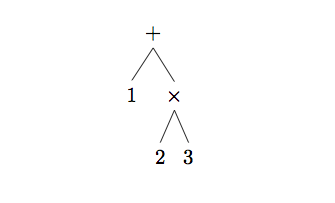
\includegraphics{kindlefig1.png}
\smspace

\noindent Notice that, in this representation, we never need parentheses -- the diagram is unambiguous. We can evaluate the expression by reducing each part in turn:

\smspace
%\Tree [.$+$ 1 [.$\times$ 2 3 ] ] \hspace{4mm}$\longrightarrow$\hspace{4mm} \Tree [.$+$ 1 6 ] \hspace{4mm}$\longrightarrow$\hspace{4mm} \Tree [.7 ]
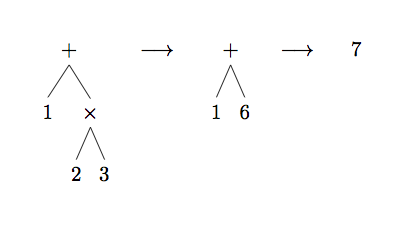
\includegraphics{kindlefig2.png}
\smspace

\noindent Here's a suitable type for such expressions:

\smspace
%\begin{center}
\noindent\fbox{\begin{minipage}{\textwidth}
$\texttt{\ptype expr =}$\\
$\texttt{\ \ Num \pof int}$\\
$\texttt{|\ Add \pof expr * expr}$\\
$\texttt{|\ Subtract \pof expr * expr}$\\
$\texttt{|\ Multiply \pof expr * expr}$\\
$\texttt{|\ Divide \pof expr * expr}$\vphantom{g}
\end{minipage}}
%\end{center}
\smspace

\noindent For example, the expression $1 + 2 * 3$ is represented in this data type as:

\smspace
\texttt{Add (Num 1, Mul (Num 2, Num 3))}
\smspace

\noindent We can now write a function to evaluate expressions:

\smspace
%\begin{center}
\noindent\fbox{\begin{minipage}{\textwidth}
\noindent\texttt{evaluate :}\textrm{ expr $\rightarrow$ \textbf{int}}\\
\\
$\texttt{\pletrec evaluate e =}$\\
$\texttt{\ \ \pmatch e \pwith}$\\
$\texttt{\ \ \ \ Num x -> x}$\\
$\texttt{\ \ |\ Add (e, e\textquotesingle ) -> evaluate e + evaluate e\textquotesingle }$\\
$\texttt{\ \ |\ Subtract (e, e\textquotesingle ) -> evaluate e - evaluate e\textquotesingle }$\\
$\texttt{\ \ |\ Multiply (e, e\textquotesingle ) -> evaluate e * evaluate e\textquotesingle }$\\
$\texttt{\ \ |\ Divide (e, e\textquotesingle ) -> evaluate e / evaluate e\textquotesingle }$\vphantom{g}
\end{minipage}}
%\end{center}
\smspace

\noindent Building our own types leads to clearer programs with more predictable behaviour, and helps us to think about a problem -- often the functions are easy to write once we have decided on appropriate types.

\clearpage
\section*{Questions}

\begin{enumerate}
  \item Design a new type \textrm{rect} for representing rectangles. Treat squares as a special case.
  \item Now write a function of type \textrm{rect $\rightarrow$ \textbf{int}} to calculate the area of a given \textrm{rect}.
  \item Write a function which rotates a \textrm{rect} such that it is at least as tall as it is wide.
  \item Use this function to write one which, given a \textrm{rect \textbf{list}}, returns another such list which has the smallest total width and whose members are sorted narrowest first.
  \item Write \texttt{take}, \texttt{drop}, and \texttt{map} functions for the \textrm{sequence} type.
  \item Extend the \textrm{expr} type and the \texttt{evaluate} function to allow raising a number to a power.
  \item Use the \textrm{option} type to deal with the problem that \texttt{Division\_by\_zero} may be raised from the \texttt{evaluate} function.
  %\item Design a type \texttt{t} to represent the OCaml data types \textbf{\textrm{int}}, \textbf{\textrm{bool}}, \textbf{\textrm{char}} as well as lists, tuples, and functions.
  %\item Now write a function of type \textrm{t} $\rightarrow$ \textbf{\textrm{string}} which returns a string representing an OCaml type as we might write it out. Pay particular attention to parentheses.
\end{enumerate}

\cleardoublepage
\thispagestyle{empty}
\chapter*{}
\noindent{\Huge So Far}\\

%\begin{multicols*}{2}
{\footnotesize
\sofarstartingoff

\vspace{\baselineskip}
\sofarfunctions

\vspace{\baselineskip}
\sofarcasebycase

\vspace{\baselineskip}
\sofarlistingthings

\vspace{\baselineskip}
\sofarsortingthings

\vspace{\baselineskip}
\sofarfunctionsuponfunctions

\vspace{\baselineskip}
\sofarwhenthingsgowrong

\vspace{\baselineskip}
\sofarlookingthingsup

\vspace{\baselineskip}
\sofarmorewithfunctions

\vspace{\baselineskip}
\sofarnewkindsofdata
}
%\end{multicols*}

\pagestyle{empty}


\chapter{Growing Trees}
\pagestyle{fancy}
\label{growingtrees}

We have used lists to represent collections of elements of like type but varying length, and tuples to represent collections of things of any type but fixed length. Another common type is the \index{binary tree}\index{tree}\textit{binary tree}, which is used to represent structures which branch, such as the arithmetical expressions we constructed in the last chapter.

How can we represent such trees using an OCaml type? When we built our version of the OCaml list type, we had two constructors -- \texttt{Cons} to hold a head and a tail, and \texttt{Nil} to represent the end of the list. With a tree, we need a version of Cons which can hold two tails -- the left and right, and we still need a version of \texttt{Nil}.

\smspace
%\begin{center}
\noindent\fbox{\begin{minipage}{\textwidth}
\noindent$\texttt{\ptype\ \textquotesingle a tree =}$\\
\noindent$\texttt{\ \ Br of \textquotesingle a * \textquotesingle a tree * \textquotesingle a tree}$\hfill\textit{branch}\\
\noindent$\texttt{|\ Lf}$\hfill\textit{leaf}
\end{minipage}}
%\end{center}
\smspace

\noindent Our type is called \textrm{tree}, and is polymorphic (can hold any kind of data at the branches). There are two constructors: \texttt{Br} for branches, which hold three things in a tuple: an element, the left sub-tree, and the right sub-tree. If it is not a \texttt{Br}, it is a \texttt{Lf} (leaf), which is used to signal that there is no left, or no right sub-tree. Here are some representations in our new type of integer trees:

\smspace

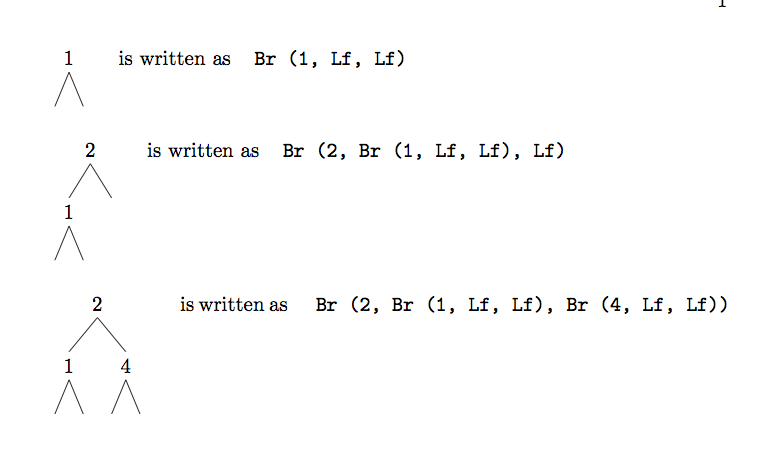
\includegraphics{kindlefig3.png}
%\Tree [.1 \phantom{3} \phantom{3} ]\hspace{4mm}is written as\hspace{4mm}\texttt{Br (1, Lf, Lf)}

%\smspace

%\Tree [.2 [.1 \phantom{3} \phantom{3} ] \phantom{3} ]\hspace{4mm}is written as\hspace{4mm}\texttt{Br (2, Br (1, Lf, Lf), Lf)}

%\smspace

%\Tree [.2 [.1 \phantom{3} \phantom{3} ] [.4 \phantom{3} \phantom{3} ] ]\hspace{4mm} is written as\hspace{4mm} \texttt{Br (2, Br (1, Lf, Lf), Br (4, Lf, Lf))}

\smspace

\noindent The empty tree is simply \texttt{Lf}. You can see now why we used abbreviated constructor names -- even small trees result in long textual representations. Let us write some simple functions on trees. To calculate the number of elements in the tree, we just count one for each branch, and zero for each leaf:

\smspace
%\begin{center}
\noindent\fbox{\begin{minipage}{0.999\textwidth}
\noindent\texttt{size :}\textrm{ $\alpha$ tree $\rightarrow$ \textbf{int}}\\
\\
$\texttt{\pletrec size tr =}$\\
$\texttt{\ \ \pmatch tr \pwith}$\\
$\texttt{\ \ \ \ Br (\_, l, r) -> 1 + size l + size r}$\\
$\texttt{\ \ |\ Lf -> 0}\vphantom{g}$
\end{minipage}}
%\end{center}
\smspace

\noindent Notice that the recursive function follows the shape of the recursive type. A similar function can be used to add up all the integers in an \textrm{\textbf{int} tree}:

\smspace
%\begin{center}
\noindent\fbox{\begin{minipage}{0.999\textwidth}
\noindent\texttt{total :}\textrm{ \textbf{int} tree $\rightarrow$ \textbf{int}}\\
\\
$\texttt{\pletrec total tr =}$\\
$\texttt{\ \ \pmatch tr \pwith}$\\
$\texttt{\ \ \ \ Br (x, l, r) -> x + total l + total r}$\\
$\texttt{\ \ |\ Lf -> 0}\vphantom{g}$
\end{minipage}}
%\end{center}
\smspace

\noindent How can we calculate the maximum depth of a tree? The depth is the longest path from the root (top) of the tree to a leaf.

\smspace
%\begin{center}
\noindent\fbox{\begin{minipage}{\textwidth}
\noindent\texttt{max :}\textrm{ \textbf{int} $\rightarrow$ \textbf{int} $\rightarrow$ \textbf{int}}\\
\noindent\texttt{maxdepth :}\textrm{ $\alpha$ tree $\rightarrow$ \textbf{int}}\\
\\
$\texttt{\plet max x y =}$\\
$\texttt{\ \ \pif x > y \pthen x \pelse y}$\\
\\
$\texttt{\pletrec maxdepth tr =}$\\
$\texttt{\ \ \pmatch tr \pwith}$\\
$\texttt{\ \ \ \ Br (\_, l, r) -> 1 + max (maxdepth l) (maxdepth r)}$\\
$\texttt{\ \ |\ Lf -> 0\vphantom{g}}$
\end{minipage}}
%\end{center}
\smspace

\noindent We defined a function \texttt{max} which returns the larger of two integers. Then, in our main function, we count a leaf as zero depth, and calculate the depth of a branch as one plus the maximum of the left and right sub-trees coming from that branch. Now consider extracting all of the elements from a tree into a list:

\smspace
%\begin{center}
\noindent\fbox{\begin{minipage}{\textwidth}
\noindent\texttt{list\_of\_tree :}\textrm{ $\alpha$ tree $\rightarrow$ $\alpha$ \textbf{list}}\\
\\
$\texttt{\pletrec list\_of\_tree tr =}$\\
$\texttt{\ \ \pmatch tr \pwith}$\\
$\texttt{\ \ \ \ Br (x, l, r) -> list\_of\_tree l @ [x] @ list\_of\_tree r}$\\
$\texttt{\ \ |\ Lf -> []}\vphantom{g}$
\end{minipage}}
%\end{center}
\smspace

\noindent Notice that we chose to put all the elements on the left branch before the current element, and all the elements in the right branch after. This is arbitrary (it is clear that there are multiple answers to the question ``How can I extract all the elements from a tree as a list?''). Before we consider real applications of trees, let us look at one more function. Here is how to map over trees:

\smspace
%\begin{center}
\noindent\fbox{\begin{minipage}{\textwidth}
\noindent\texttt{tree\_map :}\textrm{ \textmd{(}$\alpha$ $\rightarrow$ $\beta$\textmd{)} $\rightarrow$ $\alpha$ tree $\rightarrow$ $\beta$ tree}\\
\\
$\texttt{\pletrec tree\_map f tr =}$\\
$\texttt{\ \ \pmatch tr \pwith}$\\
$\texttt{\ \ \ \ Br (x, l, r) -> Br (f x, tree\_map f l, tree\_map f r)}$\\
$\texttt{\ \ |\ Lf -> Lf\vphantom{g}}$
\end{minipage}}
%\end{center}
\smspace

\noindent Notice the similarity to our \texttt{map} function for lists, both in the type and the definition.

\section*{Using trees to build better dictionaries}

\index{tree!for dictionaries}We have seen that arithmetic expressions can be drawn as trees on paper, and we have designed an OCaml data type for binary trees to hold any kind of element. Now it is time to introduce the most important application of trees: the \index{tree!binary search}\index{binary search tree}\textit{binary search tree}, which is another way of implementing the dictionary \index{data structure}\textit{data structure} we described in Chapter \ref{lookingthingsup}. 

The most important advantage of a tree is that it is often very much easier to reach a given element. When searching in a dictionary defined as a list, it took on average time proportional to the number of items in the dictionary to find a value for a key (the position of the required entry is, on average, halfway along the list). If we use a binary tree, and if it is reasonably nicely balanced in shape, that time can be reduced to the logarithm base two of the number of elements in the dictionary. Can you see why?

We can use our existing \textrm{tree} type. In the case of a dictionary, it will have type \textrm{\textmd{(}$\alpha$ $\times$ $\beta$\textmd{)} tree}, in other words a tree of key-value pairs where the keys have some type \textrm{$\alpha$} and the values some type \textrm{$\beta$}. For this example, we are going to be using another built-in type, \textrm{\textbf{string}}. A \index{string@\textrm{\textbf{string}}}\index{string}string is a sequence of characters written between double quotation marks. We have seen these as messages attached to exceptions, but they are a basic OCaml type too.

So, our tree representing a dictionary mapping integers like \texttt{1} to their spellings like \texttt{``one''} would have type \textrm{\textmd{(}\textbf{int} $\times$ \textbf{string}\textmd{)} tree}:

\smspace
%\Tree [.\texttt{(3, "three")} [.\texttt{(1, "one")} \phantom{a} [.\texttt{(2, "two")} \phantom{a} \phantom{a} ] ] [.\texttt{(4, "four")} \phantom{a} \phantom{a} ] ]
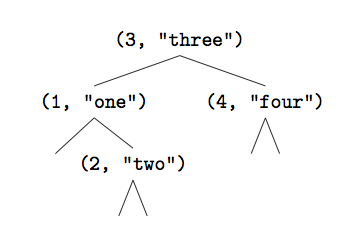
\includegraphics{kindlefig4.png}
\smspace

\noindent which would be written as

\smspace
{\footnotesize\texttt{Br ((3, "three"), Br ((1, "one"), Lf, Br ((2, "two"), Lf,
Lf)), Br ((4, "four"), Lf, Lf))}}
\smspace

\noindent If we arrange the tree such that, at each branch, everything to the left has a key less than the key at the branch, and everything to the right has a key greater than that at the branch, we have a \textit{binary search tree}.

Lookup is simple: start at the top, and if we have not found the key we are looking for, go left or right depending upon whether the required key is smaller or larger than the value at the current branch. If we reach a leaf, the key was not in the tree (assuming the tree is a well-formed binary search tree), and we raise an exception.

\smspace
%\begin{center}
\noindent\fbox{\begin{minipage}{\textwidth}
\noindent\texttt{lookup :}\textrm{ \textmd{(}$\alpha \times \beta$\textmd{)} tree $\rightarrow$ $\alpha$ $\rightarrow$ $\beta$}\\
\\
$\texttt{\pletrec lookup tr k =}$\\
$\texttt{\ \ \pmatch tr \pwith}$\\
$\texttt{\ \ \ \ Lf -> \praise Not\_found}$\\
$\texttt{\ \ |\ Br ((k\textquotesingle , v), l, r) ->}$\\
$\texttt{\ \ \ \ \ \ \pif k = k\textquotesingle\ \pthen v}$\hfill\makebox{\textit{found the key -- return the value}}\\
$\texttt{\ \ \ \ \ \ \pelse \pif k < k\textquotesingle\ \pthen lookup l k}$\hfill\makebox{\textit{go left}}\\
$\texttt{\ \ \ \ \ \ \pelse lookup r k}$\hfill\makebox{\textit{go right}} 
\end{minipage}}
%\end{center}
\smspace

\noindent Alternatively, we may use the \textrm{option} type to avoid exceptions:

\smspace
%\begin{center}
\noindent\fbox{\begin{minipage}{\textwidth}
\noindent\texttt{lookup :}\textrm{ \textmd{(}$\alpha \times \beta$\textmd{)} tree $\rightarrow$ $\alpha$ $\rightarrow$ $\beta$ \textrm{option}}\\
\\
$\texttt{\pletrec lookup tr k =}$\\
$\texttt{\ \ \pmatch tr \pwith}$\\
$\texttt{\ \ \ \ Lf -> None}$\\
$\texttt{\ \ |\ Br ((k\textquotesingle , v), l, r) ->}$\\
$\texttt{\ \ \ \ \ \ \pif k = k\textquotesingle\ \pthen Some v}$\hfill\makebox{\textit{found the key -- return the value}}\\
$\texttt{\ \ \ \ \ \ \pelse \pif k < k\textquotesingle\ \pthen lookup l k}$\hfill\makebox{\textit{go left}}\\
$\texttt{\ \ \ \ \ \ \pelse lookup r k}$\hfill\makebox{\textit{go right}} 
\end{minipage}}
%\end{center}
\smspace

\noindent How can we insert a new key-value pair into an existing tree? We can find the position to insert by using the same procedure as the lookup function -- going left or right at each branch as appropriate. If we find an equal key, we put our new value there instead. Otherwise, we will end up at a leaf, and this is the insertion point -- thus, if the key is not in the dictionary when \texttt{insert} is used, it will be added in place of an existing leaf.

\smspace
%\begin{center}
\noindent\fbox{\begin{minipage}{\textwidth}
\noindent\texttt{insert :}\textrm{ \textmd{(}$\alpha \times \beta$\textmd{)} tree $\rightarrow$ $\alpha$ $\rightarrow$ $\beta$ $\rightarrow$ \textmd{(}$\alpha \times \beta$\textmd{)} tree}\\
\\
$\texttt{\pletrec insert tr k v =}$\\
$\texttt{\ \ \pmatch tr \pwith}$\\
$\texttt{\ \ \ \ Lf -> Br ((k, v), Lf, Lf)}$\hfill\makebox{\textit{insert at leaf}}\\
$\texttt{\ \ |\ Br ((k\textquotesingle , v\textquotesingle ), l, r) ->}$\\
$\texttt{\ \ \ \ \ \ \pif k = k\textquotesingle\ \pthen Br ((k, v), l, r)}$\hfill\makebox{\textit{replace value}}\\
$\texttt{\ \ \ \ \ \ \pelse \pif k < k\textquotesingle\ \pthen Br ((k\textquotesingle , v\textquotesingle ), insert l k v,  r)}$\hfill\makebox{\textit{go left}}\\
$\texttt{\ \ \ \ \ \ \pelse Br ((k\textquotesingle , v\textquotesingle ), l, insert r k v)}$\hfill\makebox{\textit{go right}} 
\end{minipage}}
%\end{center}
\smspace

\noindent For example, if we wish to insert the value \texttt{"zero"} for the key \texttt{0} in the tree drawn above, we would obtain

\smspace
%\Tree [.\texttt{(3, "three")} [.\texttt{(1, "one")} [.\texttt{(0, "zero")} \phantom{a} \phantom{a} ] [.\texttt{(2, "two")} \phantom{a} \phantom{a} ] ] [.\texttt{(4, "four")} \phantom{a} \phantom{a} ] ]
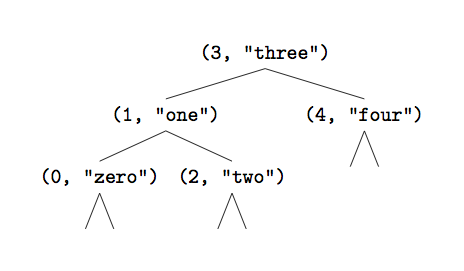
\includegraphics{kindlefig5.png}
\smspace

\noindent The shape of the tree is dependent upon the order of insertions into the tree -- if they are in order (or reverse order), we obtain a rather inefficient tree -- no better a dictionary than a list in fact. However, on average, we obtain a reasonably balanced tree, and logarithmic lookup and insertion times.

Lists and trees are examples of data structures. The design of an algorithm and its data structures are intimately connected. 

\clearpage
\section*{Questions}

\begin{enumerate}
  \item Write a function of type \textrm{$\alpha$ $\rightarrow$ $\alpha$ tree $\rightarrow$ \textbf{bool}} to determine if a given element is in a tree.
  \item Write a function which flips a tree left to right such that, if it were drawn on paper, it would appear to be a mirror image. 
  \item Write a function to determine if two trees have the same shape,
    irrespective of the actual values of the elements.
  \item Write a function \texttt{tree\_of\_list} which builds a tree representation of a dictionary from a list representation of a dictionary.
  \item Write a function to combine two dictionaries represented as trees into one. In the case of clashing keys, prefer the value from the first dictionary.  \item Can you define a type for trees which, instead of branching exactly two ways each time, can branch zero or more ways, possibly different at each branch? Write simple functions like \texttt{size}, \texttt{total}, and \texttt{map} using your new type of tree.
\end{enumerate}

\cleardoublepage
\thispagestyle{empty}
\chapter*{}
\noindent{\Huge So Far}\\

%\begin{multicols*}{2}
{\footnotesize
\sofarstartingoff

\vspace{\baselineskip}
\sofarfunctions

\vspace{\baselineskip}
\sofarcasebycase

\vspace{\baselineskip}
\sofarlistingthings

\vspace{\baselineskip}
\sofarsortingthings

\vspace{\baselineskip}
\sofarfunctionsuponfunctions

\vspace{\baselineskip}
\sofarwhenthingsgowrong

\vspace{\baselineskip}
\sofarlookingthingsup

\vspace{\baselineskip}
\sofarmorewithfunctions

\vspace{\baselineskip}
\sofarnewkindsofdata

\vspace{\baselineskip}
\sofargrowingtrees
}
%\end{multicols*}

\pagestyle{empty}


\chapter{In and Out}
\pagestyle{fancy}
\label{inandout}

We have considered a function (and indeed, a whole program composed of many functions) to take a chunk of data, do some calculations, and then produce a result. This assumption has allowed us to write neat, easily understood programs.

However, some computer programs do not have all data available at the beginning of the program (or even the beginning of a given function). The user might provide new data interactively, or the program might fetch data from the internet, or two or more programs might communicate with one another in real time.

We must learn how to write such programs, whilst understanding the utility of restricting such complications to as small a part of the program as possible -- interactivity turns out to be surprisingly hard to reason about, since the result of a function may no longer depend only on its initial argument.

\subsection*{Writing to the screen}

OCaml has a built-in function \texttt{print\_int} which prints an integer to the screen:

\smspace
\noindent\verb!        OCaml!\\
\noindent\\
\noindent\verb!# print_int 100;;!\\
\noindent\verb!100- : unit = ()!
\smspace

\noindent\index{printing to the screen}What is the type of this function? Well, it is a function, and it takes an integer as its argument. It prints the integer to the screen, and then returns\ldots what? Nothing! OCaml has a special type to represent nothing, called \textbf{\textrm{unit}}. There is exactly one thing of type \index{unit}\textrm{\textbf{unit}} which is written \texttt{()} and is called ``unit''. So, the function \texttt{print\_int} has type \textrm{\textbf{int} $\rightarrow$ \textbf{unit}}.

There is another built-in function \texttt{print\_string} of type \textrm{\textbf{string} $\rightarrow$ \textbf{unit}} to print a string, and another \texttt{print\_newline} to move to the next line. This function has type \textrm{\textbf{unit} $\rightarrow$ \textbf{unit}} because it requires no substantive argument and produces no useful result. \index{side-effect}It is only wanted for its ``side-effect''.

We can produce several side-effects, one after another, using the \index{;@\texttt{;}}\texttt{;} symbol. This evaluates the expression on its left hand side, throws away the result (which will normally be \textrm{\textbf{unit}} anyway), and then evaluates the expression to its right hand side, returning the result (which is often \textbf{\textrm{unit}} too). The type of the expression $x$ \texttt{;} $y$ is thus the type of $y$. For example, we can write a function to write to the screen an \textrm{\textbf{int} $\times$ \textbf{string}} pair as an integer on one line, followed by a string on another:

\smspace
%\begin{center}
\noindent\fbox{\begin{minipage}{\textwidth}
\noindent\texttt{print\_dict\_entry :}\textrm{ \textbf{int} $\times$ \textbf{string} $\rightarrow$ \textbf{unit}}\\
\\
$\texttt{\plet print\_dict\_entry (k, v) =}$\\
$\texttt{\ \ print\_int k ; print\_newline () ; print\_string v ; print\_newline ()}$\vphantom{g}
\end{minipage}}
%\end{center}
\smspace

\noindent Notice we have added a second call to \texttt{print\_newline}, so that our function can be called several times in a row without intervening calls to \texttt{print\_newline}. We wrote the function applications all on one line to emphasize that \texttt{;} behaves a little like an operator. However, for convenience, we would normally write it like this:

\smspace
%\begin{center}
\noindent\fbox{\begin{minipage}{0.999\textwidth}
\noindent\texttt{print\_dict\_entry :}\textrm{ \textbf{int} $\times$ \textbf{string} $\rightarrow$ \textbf{unit}}\\
\\
$\texttt{\plet print\_dict\_entry (k, v) =}$\\
$\texttt{\ \ print\_int k;}$\\
$\texttt{\ \ print\_newline ();}$\\
$\texttt{\ \ print\_string v;}$\\
$\texttt{\ \ print\_newline ()}$\vphantom{g}
\end{minipage}}
%\end{center}
\smspace

\noindent This makes it look rather like \texttt{;} is used to end each expression, but just remember that \texttt{;} is a bit like an operator -- notice that there is no \texttt{;} after the last \texttt{print\_newline\! ()}. Let us see how \texttt{print\_dict\_entry} is used in practice:

\smspace
\noindent\verb!        OCaml!\\
\noindent\\
\noindent\verb!# print_dict_entry (1, "one");;!\\
\noindent\verb!1!\\
\noindent\verb!one!\\
\noindent\verb!- : unit = ()!
\smspace


\noindent How might we print a whole dictionary (represented as a list of entries) this way? Well, we could write our own function to iterate over all the entries:

\smspace
%\begin{center}
\noindent\fbox{\begin{minipage}{\textwidth}
\noindent\texttt{print\_dict :}\textrm{ \textmd{(}\textbf{int} $\times$ \textbf{string}\textmd{)} \textbf{list} $\rightarrow$ \textbf{unit}}\\
\\
$\texttt{\pletrec print\_dict d =}$\\
$\texttt{\ \ \pmatch d \pwith}$\\
$\texttt{\ \ \ \ [] -> ()}$\hfill\makebox{\textit{do nothing; just return unit}}\\
$\texttt{\ \ |\ h::t -> print\_dict\_entry h; print\_dict t}$\hfill\makebox{\textit{do this one, and move on}}\vphantom{g}
\end{minipage}}
%\end{center}
\smspace

\noindent Better, we can extract this method into a more general one, for doing an action on each element of a list:

\smspace
%\begin{center}
\noindent\fbox{\begin{minipage}{\textwidth}
\noindent\texttt{iter :}\textrm{ \textmd{(}$\alpha$ $\rightarrow$ $\beta$\textmd{)} $\rightarrow$ $\alpha$ \textbf{list} $\rightarrow$ \textbf{unit}}\\
\\
$\texttt{\pletrec iter f l =}$\\
$\texttt{\ \ \pmatch l \pwith}$\\
$\texttt{\ \ \ \ [] -> ()}$\hfill\makebox{\textit{do nothing; just return unit}}\\
$\texttt{\ \ |\ h::t -> f h; iter f t}$\hfill\makebox{\textit{do this one, and move on}}\vphantom{g}
\end{minipage}}
%\end{center}
\smspace

\noindent Normally $\beta$ will be \textrm{\textbf{unit}}. Now we can redefine \texttt{print\_dict} using \texttt{iter}:

\smspace
%\begin{center}
\noindent\fbox{\begin{minipage}{\textwidth}
\noindent\texttt{print\_dict :}\textrm{ \textmd{(}\textbf{int} $\times$ \textbf{string}\textmd{)} \textbf{list} $\rightarrow$ \textbf{unit}}\\
\\
$\texttt{\plet print\_dict d =}$\\
$\texttt{\ \ iter print\_dict\_entry d}$\\
\\
\textit{or even\ldots}\\
\\
$\texttt{\plet print\_dict =}$\\
$\texttt{\ \ iter print\_dict\_entry}$\vphantom{g}
\end{minipage}}
%\end{center}
\smspace

\noindent For example:

\smspace
\noindent\verb!        OCaml!\\
\noindent\\
\noindent\verb!# print_dict [(1, "one"); (2, "two"); (3, "three")];;!\\
\noindent\verb!1!\\
\noindent\verb!one!\\
\noindent\verb!2!\\
\noindent\verb!two!\\
\noindent\verb!3!\\
\noindent\verb!three!\\
\noindent\verb!- : unit = ()!

\subsection*{Reading from the keyboard}
\index{keyboard}
Now we should like to write a function to read a dictionary as an \textrm{\textmd{(}\textbf{int} $\times$ \textbf{string}\textmd{)} \textbf{list}}. We will use two built-in OCaml functions. The function \texttt{read\_int} of type \textrm{\textbf{unit} $\rightarrow$ \textbf{int}} waits for the user to type in an integer and press the Enter key. The integer is then returned. The function \texttt{read\_line} of type \textrm{\textbf{unit} $\rightarrow$ \textbf{string}} waits for the user to type any string and press the enter key, returning the string.

We want the user to enter a series of keys and values (integers and strings), one per line. They will enter zero for the integer to indicate no more input. Our function will take no argument, and return a dictionary of integers and strings, so its type will be \textrm{\textbf{unit} $\rightarrow$ \textmd{(}\textbf{int} $\times$ \textbf{string}\textmd{)} \textbf{list}}.

\smspace
%\begin{center}
\noindent\fbox{\begin{minipage}{\textwidth}
\noindent\texttt{read\_dict :}\textrm{ \textbf{unit} $\rightarrow$ \textmd{(}\textbf{int} $\times$ \textbf{string}\textmd{)} \textbf{list}}\\
\\
$\texttt{\pletrec read\_dict () =}$\\
$\texttt{\ \ \plet i = read\_int () \pin}$\hfill\makebox{\textit{read an integer}}\\
$\texttt{\ \ \ \ \pif i = 0 \pthen [] \pelse}$\hfill\makebox{\textit{if zero, we are done}}\\
$\texttt{\ \ \ \ \ \ \plet name = read\_line () \pin}$\hfill\makebox{\textit{otherwise, read a name too}}\\
$\texttt{\ \ \ \ \ \ \ \ (i, name) ::\ read\_dict ()}$\hfill\makebox{\textit{build a dictionary entry, fetch another}}\vphantom{g}
\end{minipage}}
%\end{center}
\smspace

\noindent We can run this function and type in some suitable values:

\newpage %to remove orphan

\smspace
\noindent\verb!        OCaml!\\
\noindent\\
\noindent\verb!# read_dict ();;!\\
\noindent\verb!1!\\
\noindent\verb!oak!\\
\noindent\verb!2!\\
\noindent\verb!ash!\\
\noindent\verb!3!\\
\noindent\verb!elm!\\
\noindent\verb!0!\\
\noindent\verb!- : (int * string) list =!\\
\noindent\verb![(1, "oak"); (2, "ash"); (3, "elm")]!
\smspace

\noindent But there is a problem. What happens if we type in something which is not an integer when an integer is expected?

\smspace
\noindent\verb!        OCaml!\\
\noindent\\
\noindent\verb!# read_dict ();;!\\
\noindent\verb!1!\\
\noindent\verb!oak!\\
\noindent\verb!ash!\\
\noindent\verb!Exception: Failure "int_of_string".!
\smspace

\noindent We must handle this exception, and ask the user to try again. Here's a revised function:

\smspace
%\begin{center}
\noindent\fbox{\begin{minipage}{\textwidth}
\noindent\texttt{read\_dict :}\textrm{ \textbf{unit} $\rightarrow$ \textmd{(}\textbf{int} $\times$ \textbf{string}\textmd{)} \textbf{list}}\\
\\
$\texttt{\pletrec read\_dict () =}$\\
$\texttt{\ \ \ptry}$\\
$\texttt{\ \ \ \ \plet i = read\_int () \pin}$\hfill\makebox{\textit{read an integer}}\\
$\texttt{\ \ \ \ \ \ \pif i = 0 \pthen [] \pelse}$\hfill\makebox{\textit{if zero, we are done}}\\
$\texttt{\ \ \ \ \ \ \ \ \plet name = read\_line () \pin}$\hfill\makebox{\textit{otherwise, read a name too}}\\
$\texttt{\ \ \ \ \ \ \ \ \ \ (i, name) ::\ read\_dict ()}$\hfill\makebox{\textit{build a dictionary entry, fetch another}}\\
$\texttt{\ \ \pwith}$\\
$\texttt{\ \ \ \ Failure \_ ->}$\\
$\texttt{\ \ \ \ \ \ print\_string "This is not a valid integer.\ Please try again.";}$\\
$\texttt{\ \ \ \ \ \ print\_newline ();}$\\
$\texttt{\ \ \ \ \ \ read\_dict ()}$\vphantom{g}
\end{minipage}}
%\end{center}
\smspace

\noindent Now, typing mistakes can be fixed interactively:

\smspace
\noindent\verb!        OCaml!\\
\noindent\\
\noindent\verb!# read_dict ();;!\\
\noindent\verb!1!\\
\noindent\verb!oak!\\
\noindent\verb!ash!\\ 
\noindent\verb!This is not a valid integer. Please try again.!\\
\noindent\verb!2!\\
\noindent\verb!ash!\\
\noindent\verb!3!\\
\noindent\verb!elm!\\
\noindent\verb!0!\\
\noindent\verb!- : (int * string) list =!\\
\noindent\verb![(1, "oak"); (2, "ash"); (3, "elm")]!

\subsection*{Using files}

It is inconvenient to have to type new data sets in each time, so we will write functions to store a dictionary to a file, and then to read it back out again. 

\index{in\_channel@\textbf{\textrm{in\raisebox{2pt}{\_}channel}}}\index{out\_channel@\textbf{\textrm{out\raisebox{2pt}{\_}channel}}}OCaml has some basic functions to help us read and write from places data can be stored, such as files. Places we can read from have type \textrm{\textbf{in\raisebox{2pt}{\_}channel}} and places we can write to have type \textrm{\textbf{out\raisebox{2pt}{\_}channel}}. Here are functions for writing a dictionary of type \textrm{\textmd{(}\textbf{int} $\times$ \textbf{string}\textmd{)}} to a channel: 

\smspace
%\begin{center}
\noindent\fbox{\begin{minipage}{\textwidth}
\noindent\texttt{entry\_to\_channel :}\textrm{ \textbf{out\raisebox{2pt}{\_}channel} $\rightarrow$ \textmd{(}\textbf{int} $\times$ \textbf{string}\textmd{)} $\rightarrow$ \textbf{unit}}\\
\noindent\texttt{dictionary\_to\_channel :}\textrm{ \textbf{out\raisebox{2pt}{\_}channel} $\rightarrow$ \textmd{(}\textbf{int} $\times$ \textbf{string}\textmd{)} \textbf{list} $\rightarrow$ \textbf{unit}}\\
\\
$\texttt{\plet entry\_to\_channel ch (k, v) =}$\\
$\texttt{\ \ output\_string ch (string\_of\_int k);}$\\
$\texttt{\ \ output\_char ch \textquotesingle\textbackslash n\textquotesingle ;}$\\
$\texttt{\ \ output\_string ch v;}$\\
$\texttt{\ \ output\_char ch \textquotesingle\textbackslash n\textquotesingle}$\\
\\
$\texttt{\plet dictionary\_to\_channel ch d =}$\\
$\texttt{\ \ iter (entry\_to\_channel ch) d}$\vphantom{g}
\end{minipage}}
%\end{center}
\smspace

\noindent We are using the functions \texttt{output\_string} and \texttt{output\_char} to write the data in the same format we used to print it to the screen. There is no \texttt{output\_int} function, so we have used the built-in \texttt{string\_of\_int} function to build a string from the integer. The character \texttt{\textquotesingle\textbackslash n\textquotesingle} is a special one, representing moving to the next line (there is no \texttt{output\_newline} function).

How do we obtain such a channel? The function \texttt{open\_out} gives an output channel for filename given as a string. It has type \textrm{\textbf{string $\rightarrow$ out\raisebox{2pt}{\_}channel}}. After we have written the contents to the file, we must call \texttt{close\_out} (which has type \textrm{\textbf{out\raisebox{2pt}{\_}channel} $\rightarrow$ \textbf{unit}}) to properly \index{file}close the file.


\smspace
%\begin{center}
\noindent\fbox{\begin{minipage}{\textwidth}
\noindent\texttt{dictionary\_to\_file :}\textrm{ \textbf{string} $\rightarrow$ \textmd{(}\textbf{int} $\times$ \textbf{string}\textmd{)} \textbf{list} $\rightarrow$ \textbf{unit}}\\
\\
$\texttt{\plet dictionary\_to\_file filename dict =}$\\
$\texttt{\ \ \plet ch = open\_out filename \pin}$\\
$\texttt{\ \ \ \ dictionary\_to\_channel ch dict;}$\\
$\texttt{\ \ \ \ close\_out ch}$\vphantom{g}
\end{minipage}}
%\end{center}
\smspace

\noindent After running this function, you should find a file of the chosen name on your computer in the same folder from which you are running OCaml. If you are not sure where the file is being put, consult the documentation for your OCaml implementation, or use a full file path such as \texttt{"C:/file.txt"} or \texttt{"/home/yourname/file.txt"}, again depending on your system. In the following example, we are reading a dictionary from the user and writing it to file as \texttt{file.txt}:

\smspace
\noindent\verb!        OCaml!\\
\noindent\\
\noindent\verb!# dictionary_to_file "file.txt" (read_dict ());;!\\
\noindent\verb!1!\\
\noindent\verb!oak!\\
\noindent\verb!2!\\
\noindent\verb!ash!\\
\noindent\verb!3!\\
\noindent\verb!elm!\\
\noindent\verb!0!\\
\noindent\verb!- : unit!
\smspace

\noindent Now we have written a file, we can read it back in:

\smspace
%\begin{center}
\noindent\fbox{\begin{minipage}{\textwidth}
\noindent\texttt{entry\_of\_channel :}\textrm{ \textbf{in\raisebox{2pt}{\_}channel} $\rightarrow$ \textmd{(}\textbf{int} $\times$ \textbf{string}\textmd{)}}\\
\noindent\texttt{dictionary\_of\_channel :}\textrm{ \textbf{in\raisebox{2pt}{\_}channel} $\rightarrow$ \textmd{(}\textbf{int} $\times$ \textbf{string}\textmd{)} \textbf{list}}\\
\\
$\texttt{\plet entry\_of\_channel ch =}$\\
$\texttt{\ \ \plet number = input\_line ch \pin}$\\
$\texttt{\ \ \ \ \plet name = input\_line ch \pin}$\\
$\texttt{\ \ \ \ \ \ (int\_of\_string number, name)}$\\
\\
$\texttt{\pletrec dictionary\_of\_channel ch =}$\\
$\texttt{\ \ \ptry}$\\
$\texttt{\ \ \ \ \plet e = entry\_of\_channel ch \pin}$\\
$\texttt{\ \ \ \ \ \ e ::\ dictionary\_of\_channel ch}$\\
$\texttt{\ \ \pwith}$\\
$\texttt{\ \ \ \ End\_of\_file -> []}$\vphantom{g}
\end{minipage}}
%\end{center}
\smspace

\noindent We have written a function \texttt{entry\_of\_channel} to read a single integer and string (one element of our dictionary) from an input channel using the built-in functions \texttt{input\_line} and \texttt{int\_of\_string}, and a function \texttt{dictionary\_of\_channel} to read all of them as a dictionary. It makes use of the built-in exception \index{End\_of\_file@\texttt{End\_of\_file}}\texttt{End\_of\_file} to detect when there is no more in the file. Now, we can build the main function to read our dictionary from the file:

\smspace
%\begin{center}
\noindent\fbox{\begin{minipage}{\textwidth}
\noindent\texttt{dictionary\_of\_file :}\textrm{ \textbf{string} $\rightarrow$ \textmd{(}\textbf{int} $\times$ \textbf{string}\textmd{)} \textbf{list}}\\
\\
$\texttt{\plet dictionary\_of\_file filename =}$\\
$\texttt{\ \ \plet ch = open\_in filename \pin}$\\
$\texttt{\ \ \ \ \plet dict = dictionary\_of\_channel ch \pin}$\\
$\texttt{\ \ \ \ \ \ close\_in ch;}$\\
$\texttt{\ \ \ \ \ \ dict}$\vphantom{g}
\end{minipage}}
%\end{center}
\smspace

{\hyphenpenalty=10000\begin{sloppypar}
\noindent The process is the same as for \texttt{dictionary\_to\_file} but we use \texttt{open\_in} and \texttt{close\_in} instead of \texttt{open\_out} and \texttt{close\_out}.
\end{sloppypar}}

\smspace
\noindent\verb!        OCaml!\\
\noindent\\
\noindent\verb!# dictionary_of_file "file.txt";;!\\
\noindent\verb!- : (int * string) list =!\\
\noindent\verb![(1, "oak"); (2, "ash"); (3, "elm")]!

\subsection*{Summary of functions}

We have introduced the types \textrm{\textbf{unit}}, \textrm{\textbf{in\raisebox{2pt}{\_}channel}}, and \textrm{\textbf{out\raisebox{2pt}{\_}channel}}, and the exception \texttt{End\_of\_file}. Here are the functions we have used:

\vspace{8mm}
\bgroup
\def\arraystretch{1.2}
\noindent\begin{tabular}{@{}llp{0.46\textwidth}@{}} \toprule
Function & Type & Description \\\midrule
\index{print\_int@\texttt{print\_int}}\texttt{print\_int} & \textrm{\textbf{int} $\rightarrow$ \textbf{unit}} & Print an integer to the screen.\\
\index{print\_string@\texttt{print\_string}}\texttt{print\_string} & \textrm{\textbf{string} $\rightarrow$ \textbf{unit}} & Print a string to the screen.\\
\index{print\_newline@\texttt{print\_newline}}\texttt{print\_newline} & \textrm{\textbf{unit $\rightarrow$ unit}} & Print a newline character to the screen, moving to the beginning of the next line.\\
\index{read\_line@\texttt{read\_line}}\texttt{read\_line} & \textrm{\textbf{unit $\rightarrow$ string}} & Read a string from the user. The user indicates they have finished by pressing the Enter key.\\
\index{read\_int@\texttt{read\_int}}\texttt{read\_int} & \textrm{\textbf{unit $\rightarrow$ int}} & Read an integer from the user. The user indicates they have finished by pressing the Enter key. Raises \texttt{Failure\! "int\_of\_string"} if the user types something other than an integer.\\
\index{int\_of\_string@\texttt{int\_of\_string}}\texttt{int\_of\_string} & \textrm{\textbf{string $\rightarrow$ int}} & Make an integer from a string. Raises \texttt{Failure\! "int\_of\_string"} if the string does not represent a valid integer.\\
\index{string\_of\_int@\texttt{string\_of\_int}}\texttt{string\_of\_int} & \textrm{\textbf{int $\rightarrow$ string}} & Makes a string representation of an integer.\\
\index{open\_out}\texttt{open\_out} & \textrm{\textbf{string $\rightarrow$ out\raisebox{2pt}{\_}channel}} & Given a filename, open a channel for output. Raises the exception \index{Sys\_error@\texttt{Sys\_error}}\texttt{Sys\_error} if the file could not be opened.\\
\index{close\_out@\texttt{close\_out}}\texttt{close\_out} & \textrm{\textbf{out\raisebox{2pt}{\_}channel $\rightarrow$ unit}} & Close an output channel.\\
\index{open\_in@\texttt{open\_in}}\texttt{open\_in} & \textrm{\textbf{string $\rightarrow$ in\raisebox{2pt}{\_}channel}} & Given a filename, open a channel for input. Raises the exception \texttt{Sys\_error} if the file could not be opened.\\
\index{close\_in@\texttt{close\_in}}\texttt{close\_in} & \textrm{\textbf{in\raisebox{2pt}{\_}channel $\rightarrow$ unit}} & Close an input channel.\\
\index{output\_string@\texttt{output\_string}}\texttt{output\_string} & \textrm{\textbf{out\raisebox{2pt}{\_}channel $\rightarrow$ string $\rightarrow$ unit}} & Write a string to an output channel.\\
\index{output\_char@\texttt{output\_char}}\texttt{output\_char} & \textrm{\textbf{out\raisebox{2pt}{\_}channel $\rightarrow$ char $\rightarrow$ unit}} & Write a character to an output channel. \\ \bottomrule
\end{tabular}
\egroup


\clearpage
\section*{Questions}
\begin{enumerate}
\item Write a function to print a list of integers to the screen in the same format OCaml uses -- i.e. with square brackets and semicolons. 
\item Write a function to read three integers from the user, and return them as a tuple. What exceptions could be raised in the process? Handle them appropriately.
\item In our \texttt{read\_dict} function, we waited for the user to type \texttt{0} to indicate no more data. This is clumsy. Implement a new \texttt{read\_dict} function with a nicer system. Be careful to deal with possible exceptions which may be raised.
\item Write a function which, given a number $x$, prints the $x$-times table to a given file name. For example, \texttt{table\! "table.txt"\! 5} should produce a file \texttt{table.txt} containing the following:\\\\


\vspace{1mm}
\begin{tabular}{lllll}
 \verb! ! & \verb!      ! & \verb!      ! & \verb!      ! & \verb!      !\\
 \verb!1! & \verb!     2! & \verb!     3! & \verb!     4! & \verb!     5!\\
 \verb!2! & \verb!     4! & \verb!     6! & \verb!     8! & \verb!     10!\\
 \verb!3! & \verb!     6! & \verb!     9! & \verb!     12! & \verb!     15!\\
 \verb!4! & \verb!     8! & \verb!     12! & \verb!     16! & \verb!     20!\\
 \verb!5! & \verb!     10! & \verb!     15! & \verb!     20! & \verb!     25!
\end{tabular}
\vspace{1mm}

\noindent Adding the special tabulation character \texttt{\upquote{\textbackslash t}} after each number will line up the columns.
\item Write a function to count the number of lines in a given file.
\item Write a function \texttt{copy\_file} of type \textrm{\textbf{string} $\rightarrow$ \textbf{string} $\rightarrow$ \textbf{unit}} which copies a file line by line. For example, \texttt{copy\_file\! "a.txt"\! "b.txt"} should produce a file \texttt{b.txt} identical to \texttt{a.txt}. Make sure you deal with the case where the file \texttt{a.txt} cannot be found, or where \texttt{b.txt} cannot be created or filled. 
\end{enumerate}

\cleardoublepage
\thispagestyle{empty}
\chapter*{}
\noindent{\Huge So Far}\\

%\begin{multicols*}{2}
{\footnotesize
\sofarstartingoff

\vspace{\baselineskip}
\sofarfunctions

\vspace{\baselineskip}
\sofarcasebycase

\vspace{\baselineskip}
\sofarlistingthings

\vspace{\baselineskip}
\sofarsortingthings

\vspace{\baselineskip}
\sofarfunctionsuponfunctions

\vspace{\baselineskip}
\sofarwhenthingsgowrong

\vspace{\baselineskip}
\sofarlookingthingsup

\vspace{\baselineskip}
\sofarmorewithfunctions

\vspace{\baselineskip}
\sofarnewkindsofdata

\vspace{\baselineskip}
\sofargrowingtrees

\vspace{\baselineskip}
\sofarinandout
}
%\end{multicols*}

\pagestyle{empty}


\chapter{Putting Things in Boxes}
\pagestyle{fancy}
\label{puttingthingsinboxes}

So far, we have considered ``pure'' functions which have no side-effects, and functions which have the side-effect of reading or writing information to and from, for example, files. When we assigned a value to a name, that value could never change. Sometimes, it is convenient to allow the value of a name to be changed -- some algorithms are more naturally expressed in this way.

OCaml provides a construct known as a \index{ref@\textbf{\textrm{ref}}}\index{ref@\texttt{ref}}\index{reference}\textit{reference} which is a box in which we can store a value. We build a reference using the built-in function \texttt{ref} of type \textrm{\textbf{$\alpha$ $\rightarrow$ $\alpha$ ref}}. For example, let us build a reference with initial contents $0$. It will have type \textrm{\textbf{int ref}}.

\smspace
\noindent\verb!        OCaml!\\
\noindent\\
\noindent\verb!# let x = ref 0;;!\\
\noindent\verb!val x : int ref = {contents = 0}!
\smspace

\noindent OCaml tells us that \texttt{x} is a reference of type \textrm{\textbf{int ref}} which currently has contents \texttt{0}. We can extract the current contents of a reference using the \texttt{!}\! operator, which has type \textrm{\textbf{$\alpha$ ref $\rightarrow$ $\alpha$}}.

\index{"!@\texttt{"!}}
\smspace
\noindent\verb$# let p = !x;;$\\
\noindent\verb!val p : int = 0!
\smspace

\noindent We can update the contents of the reference using the \texttt{:=}\, operator:

\index{:=@\texttt{:=}}
\smspace
\noindent\verb$# x := 50;;$\\
\noindent\verb!- : unit = ()!
\smspace

\noindent The \texttt{:=}\, operator has type \textrm{\textbf{$\alpha$ ref $\rightarrow$ $\alpha$ $\rightarrow$ unit}}, since it takes a reference and a new value to put in it,  puts the value in, and returns nothing. It is only useful for its side-effect. Now, we can get the contents with \texttt{!} again.

\smspace
\noindent\verb$# let q = !x;;$\\
\noindent\verb!val q : int = 50!\\
\noindent\verb$# p;;$\\
\noindent\verb!- : int = 0!
\smspace

\noindent Notice that \texttt{p} is unchanged. Here's a function to swap the contents of two references:

\smspace
%\begin{center}
\noindent\fbox{\begin{minipage}{\textwidth}
\noindent\texttt{swap :}\textbf{\textrm{ $\alpha$ ref $\rightarrow$ $\alpha$ ref $\rightarrow$ unit}}\\
\\
$\texttt{\plet swap a b =}$\\
$\texttt{\ \ \plet t = !a \pin}$\\
$\texttt{\ \ \ \ a := !b; b := t}$\vphantom{g}
\end{minipage}}
%\end{center}
\smspace

\noindent We needed to use a temporary name \texttt{t} to store the contents of \texttt{a}. Can you see why?

This type of programming, which consists of issuing a number of commands, in order, about which references are to be altered and how, is known as \index{imperative programming@{imperative\hspace{1mm}programming}}\textit{imperative programming}. OCaml provides some useful structures for imperative programming with references. We will look at these quickly now, and in a moment build a bigger example program to show why they are useful.

For readability, OCaml lets us miss out the \texttt{\pelse} part of the \texttt{\textbf{if\ \!\ldots\ \!then\ \!\ldots\ \!else\ \!\ldots}} \ construct if it would just be \texttt{()}, which is if we are doing nothing in the \textbf{\texttt{else}} case, so

\smspace
  \texttt{\pif x = 0 \pthen a := 0 \pelse ()}
\smspace

\noindent can be written as

\smspace
  \texttt{\pif x = 0 \pthen a := 0}
\smspace

\noindent and if \texttt{x} is not zero, the expression will just evaluate to \texttt{()}. Due to this, when putting imperative code inside \texttt{\textbf{if\! \ldots\ \!then\! \ldots\ \!else\! \ldots}} constructs, we need to surround the inner imperative expressions with parentheses so the meaning is unambiguous:

\smspace
%\begin{center}
\noindent\fbox{\begin{minipage}{\textwidth}
$\texttt{\pif x = y \pthen}$\\
$\texttt{\ \ (a := !a + 1;}$\\
$\texttt{\ \ \ b := !b - 1)}$\\
$\texttt{\pelse}$\\
$\texttt{\ \ c := !c + 1}$\vphantom{g}
\end{minipage}}
%\end{center}
\smspace

\noindent OCaml allows us to use \index{begin@\texttt{\textbf{begin}}}\index{end@\texttt{\textbf{end}}}\texttt{\textbf{begin}} and \texttt{\textbf{end}} instead, for readability:

\smspace
%\begin{center}
\noindent\fbox{\begin{minipage}{\textwidth}
$\texttt{\pif x = y \pthen}$\\
$\texttt{\ \ \pbegin}$\\
$\texttt{\ \ \ \ a := !a + 1;}$\\
$\texttt{\ \ \ \ b := !b - 1}$\\
$\texttt{\ \ \pend}$\\
$\texttt{\pelse}$\\
$\texttt{\ \ c := !c + 1}$\vphantom{g}
\end{minipage}}
%\end{center}

\section*{Doing it again and again}

There are two ways to repeat an action. To perform an action a fixed number of times, we use the \index{for@\texttt{\textbf{for}}}\index{to@\texttt{\textbf{to}}}\index{do@\texttt{\textbf{do}}}\index{done@\texttt{\textbf{done}}}\texttt{\textbf{for\! \ldots\ \!= \!\ldots\ \!to \ldots\ \!do \ldots\ \!done}} construct. For example,  

\smspace
  \texttt{\pfor x = 1 \pto 5 \pdo print\_int x; print\_newline () \pdone}
\smspace

\noindent evaluates the expression \texttt{print\_int\! x;\! print\_newline\! ()} five times: once where \texttt{x} is 1, once where \texttt{x} is 2 etc, so the result is:

\smspace
\noindent\verb$# for x = 1 to 5 do print_int x; print_newline () done;$\\
\noindent\verb!1!\\
\noindent\verb!2!\\
\noindent\verb!3!\\
\noindent\verb!4!\\
\noindent\verb!5!\\
\noindent\verb!- : unit = ()!
\smspace

\noindent This is known as a \index{for loop}\index{loop}``for loop''. Note that the type of the whole \texttt{\textbf{for}\! \ldots\ \!\textbf{=} \!\ldots\ \!\textbf{to} \!\ldots\ \!\textbf{do} \!\ldots\ \!\textbf{done}}\ \ expression is \textbf{\textrm{unit}} irrespective of the type of the expression(s) inside it.

There is another looping construct -- this time for evaluating an expression
repeatedly until some condition is true. This is the \
\index{while@\texttt{\textbf{while}}}\index{do@\texttt{\textbf{do}}}\index{done@\texttt{\textbf{done}}}\texttt{\textbf{while}\!
\ldots\ \!\textbf{do}\! \ldots\ \!\textbf{done}}\ \ construct. It takes a
boolean condition, and evaluates a given expression repeatedly, zero or more
times, until the boolean condition is \texttt{false}. For example, here is a function which, given a positive integer, calculates the lowest power of two greater than or equal to that number (i.e. for the argument 37, the result will be 64).

\smspace
%\begin{center}
\noindent\fbox{\begin{minipage}{\textwidth}
\noindent\texttt{smallest\_pow2 :}\textrm{\textbf{ int $\rightarrow$ int}}\\
\\
$\texttt{\plet smallest\_pow2 x =}$\\
$\texttt{\ \ \plet t = ref 1 \pin}$\hfill\makebox{\textit{start the test value at 1}}\\
$\texttt{\ \ \ \ \pwhile\ !t < x \pdo}$\hfill\makebox{\textit{each time it is less than \texttt{x}\ldots}}\\
$\texttt{\ \ \ \ \ \ t := !t * 2}$\hfill\makebox{\textit{\ldots double it}}\\
$\texttt{\ \ \ \ \pdone;}$\\
$\texttt{\ \ \ \ !t}$\hfill\makebox{\textit{the final result is the contents of \texttt{t}}}\vphantom{g}
\end{minipage}}
%\end{center}
\smspace

\noindent The \texttt{\textbf{while}} loop continues until the contents of the
reference \texttt{t} is greater than or equal to \texttt{x}. At that point, it
ends, and the contents of \texttt{t} is returned from the function. Again, note that the type of the whole \,\texttt{\textbf{while}\! \ldots\ \!\textbf{do} \!\ldots\ \!\textbf{done}}\ \! construct is \textbf{\textrm{unit}}.

\section*{Example: text file statistics}

We are going to write a program to count the number of words, sentences and lines in a text file. We shall consider the opening paragraph of Kafka's ``Metamorphosis''.

\noindent\begin{tabular}{l}
$\texttt{One morning, when Gregor Samsa woke from troubled dreams, he found}$\\
$\texttt{himself transformed in his bed into a horrible vermin.  He lay on}$\\
$\texttt{his armour-like back, and if he lifted his head a little he could}$\\
$\texttt{see his brown belly, slightly domed and divided by arches into stiff}$\\
$\texttt{sections.  The bedding was hardly able to cover it and seemed ready}$\\
$\texttt{to slide off any moment.  His many legs, pitifully thin compared}$\\
$\texttt{with the size of the rest of him, waved about helplessly as he}$\\
$\texttt{looked.}$
\end{tabular}

\noindent There are newline characters at the end of each line, save for the last. You can cut and paste or type this into a text file to try these examples out. Here, it is saved as \texttt{gregor.txt}.

We will just count lines first. To this, we will write a function \texttt{channel\_statistics} to gather the statistics by reading an input channel and printing them. Then we will have a function to open a named file, call our first function, and close it again.

\smspace
%\begin{center}
\noindent\fbox{\begin{minipage}{0.999\textwidth}
\noindent\texttt{channel\_statistics :}\textrm{\textbf{ in\raisebox{2pt}{\_}channel $\rightarrow$ unit}}\\
\noindent\texttt{file\_statistics :}\textrm{\textbf{ string $\rightarrow$ unit}}\\
\\
$\texttt{\plet channel\_statistics in\_channel =}$\\
$\texttt{\ \ \plet lines = ref 0 \pin}$\\
$\texttt{\ \ \ \ \ptry}$\\
$\texttt{\ \ \ \ \ \ \pwhile true \pdo}$\\
$\texttt{\ \ \ \ \ \ \ \ \plet line = input\_line in\_channel \pin}$\\
$\texttt{\ \ \ \ \ \ \ \ \ \ lines := !lines + 1}$\\
$\texttt{\ \ \ \ \ \ \pdone}$\\
$\texttt{\ \ \ \ \pwith}$\\
$\texttt{\ \ \ \ \ \ End\_of\_file ->}$\\
$\texttt{\ \ \ \ \ \ \ \ print\_string "There were ";}$\\
$\texttt{\ \ \ \ \ \ \ \ print\_int !lines;}$\\
$\texttt{\ \ \ \ \ \ \ \ print\_string " lines.";}$\\
$\texttt{\ \ \ \ \ \ \ \ print\_newline ()}$\\
\\
$\texttt{\plet file\_statistics name =}$\\
$\texttt{\ \ \plet channel = open\_in name \pin}$\\
$\texttt{\ \ \ \ \ptry}$\\
$\texttt{\ \ \ \ \ \ channel\_statistics channel;}$\\
$\texttt{\ \ \ \ \ \ close\_in channel}$\\
$\texttt{\ \ \ \ \pwith}$\\
$\texttt{\ \ \ \ \ \ \_ -> close\_in channel}$\vphantom{g}
\end{minipage}}
%\end{center}
\smspace

\noindent Notice the use of \texttt{true} as the condition for the \textbf{\texttt{while}} construct. This means the computation would carry on forever, except that the \texttt{End\_of\_file} exception must eventually be raised. Note also that OCaml emits  a warning when reading the \texttt{channel\_statistics} function:

\smspace
\texttt{Warning 26:\ unused variable line.}
\smspace

\noindent This is an example of a warning we can ignore -- we are not using the actual value \texttt{line} yet, since we are just counting lines without looking at their content. Running our program on the example file gives this:

\smspace
\noindent\verb!        OCaml!\\
\noindent\\
\noindent\verb!# file_statistics "gregor.txt";;!\\
\noindent\verb!There were 8 lines.!\\
\noindent\verb!- : unit = ()!
\smspace

\noindent Let us update the program to count the number of words, characters, and sentences. We will do this simplistically, assuming that the number of words can be counted by counting the number of spaces, and that the sentences can be counted by noting instances of \texttt{\upquote{.}}, \texttt{\upquote{!}}, and \texttt{\upquote{?}}. We can extend the \texttt{channel\_statistics} function appropriately -- \texttt{file\_statistics} need not change:

\smspace
%\begin{center}
\noindent\fbox{\begin{minipage}{\textwidth}
\noindent\texttt{channel\_statistics :}\textrm{\textbf{ in\raisebox{2pt}{\_}channel $\rightarrow$ unit}}\\
\\
$\texttt{\plet channel\_statistics in\_channel =}$\\
$\texttt{\ \ \plet lines = ref 0 \pin}$\\
$\texttt{\ \ \plet characters = ref 0 \pin}$\\
$\texttt{\ \ \plet words = ref 0 \pin}$\\
$\texttt{\ \ \plet sentences = ref 0 \pin}$\\
$\texttt{\ \ \ \ \ptry}$\\
$\texttt{\ \ \ \ \ \ \pwhile true \pdo}$\\
$\texttt{\ \ \ \ \ \ \ \ \plet line = input\_line in\_channel \pin}$\\
$\texttt{\ \ \ \ \ \ \ \ \ \ lines := !lines + 1;}$\\
$\texttt{\ \ \ \ \ \ \ \ \ \ characters := !characters + String.length line;}$\\
$\texttt{\ \ \ \ \ \ \ \ \ \ String.iter}$\\
$\texttt{\ \ \ \ \ \ \ \ \ \ \ \ (\pfun c ->}$\\
$\texttt{\ \ \ \ \ \ \ \ \ \ \ \ \ \ \ \pmatch c \pwith}$\\
$\texttt{\ \ \ \ \ \ \ \ \ \ \ \ \ \ \ \ \ \upquote{.}\ | \upquote{?}\ | \upquote{!}\ -> sentences := !sentences + 1}$\\
$\texttt{\ \ \ \ \ \ \ \ \ \ \ \ \ \ \ | \upquote{ } -> words := !words + 1}$\\
$\texttt{\ \ \ \ \ \ \ \ \ \ \ \ \ \ \ | \_ -> ())}$\\
$\texttt{\ \ \ \ \ \ \ \ \ \ \ \ line}$\\
$\texttt{\ \ \ \ \ \ \pdone}$\\
$\texttt{\ \ \ \ \pwith}$\\
$\texttt{\ \ \ \ \ \ End\_of\_file ->}$\\
$\texttt{\ \ \ \ \ \ \ \ print\_string "There were ";}$\\
$\texttt{\ \ \ \ \ \ \ \ print\_int !lines;}$\\
$\texttt{\ \ \ \ \ \ \ \ print\_string " lines, making up ";}$\\
$\texttt{\ \ \ \ \ \ \ \ print\_int !characters;}$\\
$\texttt{\ \ \ \ \ \ \ \ print\_string " characters with ";}$\\
$\texttt{\ \ \ \ \ \ \ \ print\_int !words;}$\\
$\texttt{\ \ \ \ \ \ \ \ print\_string " words in ";}$\\
$\texttt{\ \ \ \ \ \ \ \ print\_int !sentences;}$\\
$\texttt{\ \ \ \ \ \ \ \ print\_string " sentences.";}$\\
$\texttt{\ \ \ \ \ \ \ \ print\_newline ()}$\vphantom{g}
\end{minipage}}
%\end{center}
\smspace

\noindent We have used the built-in function \texttt{String.iter} of type \textrm{\textbf{\textmd{(}char $\rightarrow$ unit\textmd{)} $\rightarrow$ string $\rightarrow$ unit}} which calls a function we supply on each character of a string.

Substituting this version of \texttt{channel\_statistics} (if you are cutting and pasting into OCaml, be sure to also paste \texttt{file\_statistics} in again afterwards, so it uses the new \texttt{channel\_statistics}), gives the following result on our example text:

\smspace
\noindent\verb!        OCaml!\\
\noindent\\
\noindent\verb!# file_statistics "gregor.txt";;!\\
\noindent\verb!There were 8 lines, making up 464 characters with 80 words in 4 sentences.!\\
\noindent\verb!- : unit = ()!
\smspace

\subsection*{Adding character counts}

We should like to build a histogram, counting the number of times each letter of the alphabet or other character occurs. It would be tedious and unwieldy to hold a hundred or so references, and then pattern match on each possible character to increment the right one. OCaml provides a data type called \textrm{\textbf{array}} for situations like this.

An \index{array@\textbf{\textrm{array}}}\index{array}array is a place for storing a fixed number of elements of like type. We can introduce arrays by using \texttt{[|} and \texttt{|]}, with semicolons to separate the elements:

\smspace
\noindent\verb!        OCaml!\\
\noindent\\
\noindent\verb!# let a = [|1; 2; 3; 4; 5|];;!\\
\noindent\verb!val a : int array = [|1; 2; 3; 4; 5|]!
\smspace

\noindent We can access an element inside our array in constant time by giving the position of the element (known as the \index{subscript}\textit{subscript}) in parentheses, after the array name and a period:

\smspace
\noindent\verb!# a.(0);;!\\
\noindent\verb!- : int = 1!
\smspace

\noindent Notice that the first element has subscript $0$, not $1$. We can update any of the values in the array, also in constant time, like this:

\index{<-@\texttt{<-}}
\smspace
\noindent\verb!# a.(4) <- 100;;!\\
\noindent\verb!- : unit = ()!\\
\noindent\verb!# a;;!\\
\noindent\verb!a : int array = [|1; 2; 3; 4; 100|]!
\smspace

\noindent If we try to access or update an element which is not within range, an exception is raised:

\smspace
\noindent\verb!# a.(5);;!\\
\noindent\verb!Exception: Invalid_argument "index out of bounds".!
\smspace

\noindent There are some useful built-in functions for dealing with arrays. The function \texttt{Array.length} of type \textbf{\textrm{$\alpha$ array $\rightarrow$ int}} returns the length of an array:

\smspace
\noindent\verb!# Array.length a;;!\\
\noindent\verb!- : int = 5!
\smspace

\noindent In contrast to finding the length of a list, the time taken by \texttt{Array.length} is constant, since it was fixed when the array was created. The \texttt{Array.make} function is used for building an array of a given length, initialized with given values. It takes two arguments -- the length, and the initial value to be given to every element. It has type \textrm{\textbf{int $\rightarrow$ $\alpha$ $\rightarrow$ $\alpha$ array}}.

\smspace
\noindent\verb!# Array.make 6 true;;!\\
\noindent\verb!- : bool array =!\\
\noindent\verb![|true; true; true; true; true; true|]!\\
\noindent\verb!# Array.make 10 'A';;!\\
\noindent\verb!- : char array =!\\
\noindent\verb![|'A'; 'A'; 'A'; 'A'; 'A'; 'A'; 'A'; 'A'; 'A'; 'A'|]!\\
\noindent\verb!# Array.make 3 (Array.make 3 5);;!\\
\noindent\verb!- : int array array =!\\
\noindent\verb![|[|5; 5; 5|]; [|5; 5; 5|]; [|5; 5; 5|]|]!
\smspace 

\noindent Back to our original problem. We want to store a count for each possible character. We cannot subscript our arrays with characters directly, but each character has a special integer code (its so-called \index{ASCII}``ASCII code'', a common encoding of characters as integers in use since the 1960s), and we can convert to and from these using the built-in functions \texttt{int\_of\_char} and \texttt{char\_of\_int}. For example:

\smspace
\noindent\verb!        OCaml!\\
\noindent\\
\noindent\verb!# int_of_char 'C';;!\\
\noindent\verb!- : int = 67!\\
\noindent\verb!# char_of_int 67;;!\\
\noindent\verb!- : char = 'C'!\vphantom{g}
\smspace

\noindent The numbers go from 0 to 255 inclusive (they do not all represent printable characters, for example the newline character \texttt{\upquote{\textbackslash n}} has code 10). So, we can store our histogram as an integer array of length 256.

Our main function is getting rather long, so we will write a separate one which, given the completed array prints out the frequencies. If there were no instances of a particular character, no line is printed for that character.

\smspace
%\begin{center}
\noindent\fbox{\begin{minipage}{\textwidth}
\noindent\texttt{print\_histogram :}\textrm{\textbf{ int array $\rightarrow$ unit}}\\
\\
$\texttt{\plet print\_histogram arr =}$\\
$\texttt{\ \ print\_string "Character frequencies:";}$\\
$\texttt{\ \ print\_newline ();}$\\
$\texttt{\ \ \pfor x = 0 \pto 255 \pdo}$\hfill\makebox{\textit{for each character}}\\
$\texttt{\ \ \ \ \pif arr.(x) > 0 \pthen}$\hfill\makebox{\textit{only if the count is non-zero}}\\
$\texttt{\ \ \ \ \ \ \pbegin}$\\
$\texttt{\ \ \ \ \ \ \ \ print\_string "For character \textquotesingle";}$\\
$\texttt{\ \ \ \ \ \ \ \ print\_char (char\_of\_int x);}$\hfill\makebox{\textit{print the character}}\\
$\texttt{\ \ \ \ \ \ \ \ print\_string "\textquotesingle (character number ";}$\\
$\texttt{\ \ \ \ \ \ \ \ print\_int x;}$\hfill\makebox{\textit{print the character number}}\\
$\texttt{\ \ \ \ \ \ \ \ print\_string ") the count is ";}$\\
$\texttt{\ \ \ \ \ \ \ \ print\_int arr.(x);}$\hfill\makebox{\textit{print the count}}\\
$\texttt{\ \ \ \ \ \ \ \ print\_string ".";}$\\
$\texttt{\ \ \ \ \ \ \ \ print\_newline ()}$\\
$\texttt{\ \ \ \ \ \ \pend}$\\
$\texttt{\ \ \pdone}$\vphantom{g}
\end{minipage}}
%\end{center}
\smspace

\noindent This prints lines like:

\smspace
\texttt{For character \upquote{d} (character number 100) the count is 6.}
\smspace

\noindent Now, we can alter our \texttt{channel\_statistics} to create an appropriate array, and update it, once again using \texttt{String.iter}: 

\smspace
%\begin{center}
\noindent\fbox{\begin{minipage}{\textwidth}
\noindent\texttt{channel\_statistics :}\textrm{\textbf{ in\raisebox{2pt}{\_}channel $\rightarrow$ unit}}\\
\\
$\texttt{\plet channel\_statistics in\_channel =}$\\
$\texttt{\ \ \plet lines = ref 0 \pin}$\\
$\texttt{\ \ \plet characters = ref 0 \pin}$\hfill\makebox{\textit{we do not indent all these \texttt{\textbf{let}}s.}}\\
$\texttt{\ \ \plet words = ref 0 \pin}$\\
$\texttt{\ \ \plet sentences = ref 0 \pin}$\\
$\texttt{\ \ \plet histogram = Array.make 256 0 \pin}$\hfill\makebox{\textit{length 256, all elements initially 0}}\\
$\texttt{\ \ \ \ \ptry}$\\
$\texttt{\ \ \ \ \ \ \pwhile true \pdo}$\\
$\texttt{\ \ \ \ \ \ \ \ \plet line = input\_line in\_channel \pin}$\\
$\texttt{\ \ \ \ \ \ \ \ \ \ lines := !lines + 1;}$\\
$\texttt{\ \ \ \ \ \ \ \ \ \ characters := !characters + String.length line;}$\\
$\texttt{\ \ \ \ \ \ \ \ \ \ String.iter}$\\
$\texttt{\ \ \ \ \ \ \ \ \ \ \ \ (\pfun c ->}$\\
$\texttt{\ \ \ \ \ \ \ \ \ \ \ \ \ \ \ \pmatch c \pwith}$\\
$\texttt{\ \ \ \ \ \ \ \ \ \ \ \ \ \ \ \ \ \upquote{.}\ | \upquote{?}\ | \upquote{!}\ -> sentences := !sentences + 1}$\\
$\texttt{\ \ \ \ \ \ \ \ \ \ \ \ \ \ \ | \upquote{ } -> words := !words + 1}$\\
$\texttt{\ \ \ \ \ \ \ \ \ \ \ \ \ \ \ | \_ -> ())}$\\
$\texttt{\ \ \ \ \ \ \ \ \ \ \ \ line;}$\\
$\texttt{\ \ \ \ \ \ \ \ \ \ String.iter}$\hfill\makebox{\textit{for each character\ldots}}\\
$\texttt{\ \ \ \ \ \ \ \ \ \ \ \ (\pfun c ->}$\\
$\texttt{\ \ \ \ \ \ \ \ \ \ \ \ \ \ \plet i = int\_of\_char c \pin}$\\
$\texttt{\ \ \ \ \ \ \ \ \ \ \ \ \ \ \ \ histogram.(i) <- histogram.(i) + 1)}$\hfill\makebox{\textit{update histogram}}\\
$\texttt{\ \ \ \ \ \ \ \ \ \ \ \ line}$\\
$\texttt{\ \ \ \ \ \ \pdone}$\\
$\texttt{\ \ \ \ \pwith}$\\
$\texttt{\ \ \ \ \ \ End\_of\_file ->}$\\
$\texttt{\ \ \ \ \ \ \ \ print\_string "There were ";}$\\
$\texttt{\ \ \ \ \ \ \ \ print\_int !lines;}$\\
$\texttt{\ \ \ \ \ \ \ \ print\_string " lines, making up ";}$\\
$\texttt{\ \ \ \ \ \ \ \ print\_int !characters;}$\\
$\texttt{\ \ \ \ \ \ \ \ print\_string " characters with ";}$\\
$\texttt{\ \ \ \ \ \ \ \ print\_int !words;}$\\
$\texttt{\ \ \ \ \ \ \ \ print\_string " words in ";}$\\
$\texttt{\ \ \ \ \ \ \ \ print\_int !sentences;}$\\
$\texttt{\ \ \ \ \ \ \ \ print\_string " sentences.";}$\\
$\texttt{\ \ \ \ \ \ \ \ print\_newline ();}$\\
$\texttt{\ \ \ \ \ \ \ \ print\_histogram histogram}$\hfill\makebox{\textit{call histogram printer}}\vphantom{g}
\end{minipage}}
%\end{center}
\smspace

\noindent Here is the output on our text:

\smspace
\noindent\verb!        OCaml!\\
\noindent\\
\noindent\verb!# file_statistics "gregor.txt";;!\\
\verb!There were 8 lines, making up 464 characters with 80 words in 4 sentences.!\\
\verb!Character frequencies:!\\
\verb!For character ' ' (character number 32) the count is 80.!\\
\verb!For character ',' (character number 44) the count is 6.!\\
\verb!For character '-' (character number 45) the count is 1.!\\
\verb!For character '.' (character number 46) the count is 4.!\\
\verb!For character 'G' (character number 71) the count is 1.!\\
\verb!For character 'H' (character number 72) the count is 2.!\\
\verb!For character 'O' (character number 79) the count is 1.!\\
\verb!For character 'S' (character number 83) the count is 1.!\\
\verb!For character 'T' (character number 84) the count is 1.!\\
\verb!For character 'a' (character number 97) the count is 24.!\\
\verb!For character 'b' (character number 98) the count is 10.!\\
\verb!For character 'c' (character number 99) the count is 6.!\\
\verb!For character 'd' (character number 100) the count is 25.!\\
\verb!For character 'e' (character number 101) the count is 47.!\\
\verb!For character 'f' (character number 102) the count is 13.!\\
\verb!For character 'g' (character number 103) the count is 5.!\\
\verb!For character 'h' (character number 104) the count is 22.!\\
\verb!For character 'i' (character number 105) the count is 30.!\\
\verb!For character 'k' (character number 107) the count is 4.!\\
\verb!For character 'l' (character number 108) the count is 23.!\\
\verb!For character 'm' (character number 109) the count is 15.!\\
\verb!For character 'n' (character number 110) the count is 21.!\\
\verb!For character 'o' (character number 111) the count is 27.!\\
\verb!For character 'p' (character number 112) the count is 3.!\\
\verb!For character 'r' (character number 114) the count is 20.!\\
\verb!For character 's' (character number 115) the count is 24.!\\
\verb!For character 't' (character number 116) the count is 21.!\\
\verb!For character 'u' (character number 117) the count is 6.!\\
\verb!For character 'v' (character number 118) the count is 4.!\\
\verb!For character 'w' (character number 119) the count is 6.!\\
\verb!For character 'y' (character number 121) the count is 10.!\\
\verb!For character 'z' (character number 122) the count is 1.!\\
\noindent\verb!- : unit = ()!\vphantom{g}
\smspace

\noindent The most common character is the space. The most common alphabetic character is \texttt{\upquote{e}}.

\clearpage
\section*{Questions}

\begin{enumerate}
  \item Consider the expression
  
  \texttt{\textbf{let} x = ref 1 \textbf{in} \textbf{let} y = ref 2 \textbf{in} x := !x + !x; y := !x + !y; !x + !y}
  
  What references have been created? What are their initial and final values after this expression has been evaluated? What is the type of this expression? 
  \item What is the difference between \texttt{[ref\! 5;\! ref\! 5]} and \texttt{\plet \!x\! =\! ref\! 5\! \pin \![x;\! x]}? 
    
  \item Imagine that the \texttt{\textbf{for\! \!\ldots\ \!to \!\ldots\ \!do \!\ldots\ \!done}} construct did not exist. How might we create the same behaviour?
  
  \item What are the types of these expressions?
  
  \texttt{[|1; 2; 3|]}
  
  \texttt{[|true; false; true|]}
  
  \texttt{[|[|1|]|]}
  
  \texttt{[|[1; 2; 3]; [4; 5; 6]|]}
  
  \texttt{[|1; 2; 3|].(2)}
  
  \texttt{[|1; 2; 3|].(2) <- 4}
  
  \item Write a function to compute the sum of the elements in an integer array.
  
  \item Write a function to reverse the elements of an array in place (i.e. do not create a new array).
  
  \item Write a function \texttt{table} which, given an integer, builds the \textbf{\textrm{int array array}} representing the multiplication table up to that number. For example, \texttt{table\! 5} should yield:

\vspace{2mm}  
\noindent\begin{tabular}{@{}lllll@{}}
 \verb!1! & \verb!2! & \verb!3! & \verb!4! & \verb!5!\\
 \verb!2! & \verb!4! & \verb!6! & \verb!8! & \verb!10!\\
 \verb!3! & \verb!6! & \verb!9! & \verb!12! & \verb!15!\\
 \verb!4! & \verb!8! & \verb!12! & \verb!16! & \verb!20!\\
 \verb!5! & \verb!10! & \verb!15! & \verb!20! & \verb!25!
\end{tabular}
\vspace{2mm}

  There is more than one way to represent this as an array of arrays; you may choose.
  \item The ASCII codes for the lower case letters \texttt{\upquote{a}}\ldots\texttt{\upquote{z}} are 97\ldots 122, and for the upper case letters \texttt{\upquote{A}}\ldots\texttt{\upquote{Z}} they are 65\ldots 90. Use the built-in functions \texttt{int\_of\_char} and \texttt{char\_of\_int} to write functions to uppercase and lowercase a character. Non-alphabetic characters should remain unaltered.
  
  \item Comment on the accuracy of our character, word, line, and sentence statistics in the case of our example paragraph. What about in general?
  \item Choose one of the problems you have identified, and modify our program to fix it.
  
\end{enumerate}

\cleardoublepage
\thispagestyle{empty}
\chapter*{}
\noindent{\Huge So Far}\\

%\begin{multicols*}{2}
{\footnotesize
\sofarstartingoff

\vspace{\baselineskip}
\sofarfunctions

\vspace{\baselineskip}
\sofarcasebycase

\vspace{\baselineskip}
\sofarlistingthings

\vspace{\baselineskip}
\sofarsortingthings

\vspace{\baselineskip}
\sofarfunctionsuponfunctions

\vspace{\baselineskip}
\sofarwhenthingsgowrong

\vspace{\baselineskip}
\sofarlookingthingsup

\vspace{\baselineskip}
\sofarmorewithfunctions

\vspace{\baselineskip}
\sofarnewkindsofdata

\vspace{\baselineskip}
\sofargrowingtrees

\vspace{\baselineskip}
\sofarinandout

\vspace{\baselineskip}
\sofarputtingthingsinboxes
}
%\end{multicols*}

\pagestyle{empty}


\chapter{The Other Numbers}
\pagestyle{fancy}
\label{gettingreal}

The only numbers we have considered until now have been the integers. For a lot of programming tasks, they are sufficient. And, except for their limited range and the possibility of division by zero, they are easy to understand and use. However, we must now consider the \index{real number}real numbers.

It is clearly not possible to represent all numbers exactly -- they might be irrational like $\pi$ or $e$ and have no finite representation. For most uses, a representation called \index{floating-point}\textit{floating-point} is suitable, and this is how OCaml's real numbers are stored. Not all numbers can be represented exactly, but arithmetic operations are very quick.

Floating-point numbers have type \textbf{\textrm{float}}. We can write a floating-point number by including a decimal point somewhere in it. For example \verb!1.6! or \verb!2.!\!\!\ \ or \texttt{386.54123}. Negative floating-point numbers are preceded by the \verb!-.! characters just like negative integers are preceded by the \verb!-! character. Similarly, we write \index{+.@\texttt{+.}}\index{-.@\texttt{-.}}\index{*.@\texttt{*.}}\index{/.@\texttt{/.}}\verb!+.! \verb!-.! \verb!*.! \verb!/.! for the standard arithmetic operators on floating-point numbers. Exponentiation is written with the \verb!**! operator.

\smspace
\noindent\verb!        OCaml!\\
\noindent\\
\noindent\verb!# 1.5;;!\\
\verb!- : float = 1.5!\\
\verb!# 6.;;!\\
\verb!- : float = 6.!\\
\verb!# -.2.3456;;!\\
\verb!- : float = -2.3456!\\
\verb!# 1.0 +. 2.5 *. 3.0;;!\\
\verb!- : float = 8.5!\\
\verb!# 1.0 /. 1000.0;;!\\
\verb!- : float = 0.001!\\
\verb!# 1. /. 100000.;;!\\
\verb!- : float = 1e-05!\\
\verb!# 3000. ** 10.;;!\\
\verb!- : float = 5.9049e+34!\\
\verb!# 3.123 -. 3.;;!\\
\verb!- : float = 0.12300000000000022!\vphantom{g}
\smspace

\noindent Notice an example of the limits of precision in floating-point operations in the final lines. Note also that very small or very large numbers are written using scientific notation (such as \texttt{5.9049e+34} above). We can find out the range of numbers available:

\smspace
\noindent\verb!        OCaml!\\
\noindent\\
\verb!# max_float;;!\\
\verb!- : float = 1.79769313486231571e+308!\\
\verb!# min_float;;!\\
\verb!- : float = 2.22507385850720138e-308!\vphantom{g}
\smspace

\noindent Working with floating-point numbers requires care, and a comprehensive discussion is outside the scope of this book. These challenges exist in any programming language using the floating-point system. For example, evaluating \texttt{1.\!\!\!\!\! /.\!\!\!\!\! 0.}\! gives the special value \texttt{infinity} (there is no \texttt{Division\_by\_zero} exception for floating-point operations). There are other special values such as \verb!neg_infinity! and \verb!nan! (``not a number''). We will leave these complications for now -- just be aware that they are lurking and must be confronted when writing robust numerical programs.

A number of standard functions are provided, both for operating on floating-point numbers and for converting to and from them, some of which are listed here:

\smspace
\bgroup
\def\arraystretch{1.2}
\noindent\begin{tabular}{@{}llp{0.55\textwidth}@{}} \toprule
Function & Type & Description\\ \midrule
\index{sqrt@\texttt{sqrt}}\verb!sqrt! & \textrm{\textbf{float $\rightarrow$ float}} & Square root of a number.\\
\index{log@\texttt{log}}\verb!log! & \textrm{\textbf{float $\rightarrow$ float}} & Natural logarithm.\\
\index{log10@\texttt{log10}}\verb!log10! & \textrm{\textbf{float $\rightarrow$ float}} & Logarithm base ten.\\
\index{sin@\texttt{sin}}\verb!sin! & \textrm{\textbf{float $\rightarrow$ float}} & Sine of an angle, given in radians.\\
\index{cos@\texttt{cos}}\verb!cos! & \textrm{\textbf{float $\rightarrow$ float}} & Cosine of an angle, given in radians.\\
\index{tan@\texttt{tan}}\verb!tan! & \textrm{\textbf{float $\rightarrow$ float}} & Tangent of an angle, given in radians.\\
\index{atan@\texttt{atan}}\verb!atan! & \textrm{\textbf{float $\rightarrow$ float}} & Arctangent of an angle, given in radians.\\
\index{ceil@\texttt{ceil}}\verb!ceil! & \textrm{\textbf{float $\rightarrow$ float}} & Calculate the nearest whole number at least as big as a floating-point number.\\
\index{floor@\texttt{floor}}\verb!floor! & \textrm{\textbf{float $\rightarrow$ float}} & The nearest whole number at least as small as a floating-point number.\\
\index{float\_of\_int@\texttt{float\_of\_int}}\verb!float_of_int! & \textrm{\textbf{int $\rightarrow$ float}}& Convert an integer to a floating-point number.\\
\index{int\_of\_float@\texttt{int\_of\_float}}\verb!int_of_float!& \textrm{\textbf{float $\rightarrow$ int}}& Build an integer from a floating-point number, ignoring the non-integer part.\\
\index{print\_float@\texttt{print\_float}}\verb!print_float! & \textrm{\textbf{float $\rightarrow$ unit}} & Print a floating-point number to the screen.\\
\index{string\_of\_float@\texttt{string\_of\_float}}\verb!string_of_float! & \textrm{\textbf{float $\rightarrow$ string}} & Build a string from a floating-point number.\\
\index{float\_of\_string@\texttt{float\_of\_string}}\verb!float_of_string! & \textrm{\textbf{string $\rightarrow$ float}} & Build a floating-point number from a string. Raises \texttt{Failure\! "float\_of\_string"} on a bad argument. \\ \bottomrule
\end{tabular}
\egroup
\smspace

\noindent Let us write some functions with floating-point numbers. We will write some simple operations on vectors in two dimensions. We will represent a point as a pair of floating-point numbers of type \textrm{\textbf{float $\times$ float}} such as \texttt{(2.0, 3.0)}. We will represent a vector as a pair of floating-point numbers too. Now we can write a function to build a vector from one point to another, one to find the length of a vector, one to offset a point by a vector, and one to scale a vector to a given length:

\smspace
%\begin{center}
\noindent\fbox{\begin{minipage}{\textwidth}
\noindent\texttt{make\_vector :}\textbf{\textrm{ float $\times$ float $\rightarrow$ float $\times$ float $\rightarrow$ float $\times$ float}}\\
\noindent\texttt{vector\_length :}\textbf{\textrm{ float $\times$ float $\rightarrow$ float}}\\
\noindent\texttt{offset\_point :}\textbf{\textrm{ float $\times$ float $\rightarrow$ float $\times$ float $\rightarrow$ float $\times$ float}}\\
\noindent\texttt{scale\_to\_length :}\textbf{\textrm{ float $\rightarrow$ float $\times$ float $\rightarrow$ float $\times$ float}}\\
\\
$\texttt{\plet make\_vector (x0, y0) (x1, y1) =}$\\
$\texttt{\ \ (x1 -.\ x0, y1 -.\ y0)}$\\
\\
$\texttt{\plet vector\_length (x, y) =}$\\
$\texttt{\ \ sqrt (x *.\ x +.\ y *.\ y)}$\\
\\
$\texttt{\plet offset\_point (x, y) (px, py) =}$\\
$\texttt{\ \ (px +.\ x, py +.\ y)}$\\
\\
$\texttt{\plet scale\_to\_length l (a, b) =}$\\
$\texttt{\ \ \plet currentlength = vector\_length (a, b) \pin}$\\
$\texttt{\ \ \ \ \pif currentlength = 0.\ \pthen (a, b) \pelse}$\hfill\makebox{\textit{to avoid division by zero}}\\
$\texttt{\ \ \ \ \ \ \plet factor = l /.\ currentlength \pin}$\\
$\texttt{\ \ \ \ \ \ \ \ (a *.\ factor, b *.\ factor)}$\vphantom{g}
\end{minipage}}
%\end{center}
\smspace

\noindent Notice that we have to be careful about division by zero, just as with integers. We have used tuples for the points because it is easier to read this way -- we could have passed each floating-point number as a separate argument instead, of course.

Floating-point numbers are often essential, but must be used with caution. You will discover this when answering the questions for this chapter. Some of these questions require using the built-in functions listed in the table above.

\clearpage
\subsection*{Questions}
\begin{enumerate}
\item Give a function which rounds a positive floating-point number to the nearest whole number, returning another floating-point number.

\item Write a function to find the point equidistant from two given points in two dimensions.

\item Write a function to separate a floating-point number into its integer and whole parts. Return them as a tuple of type \textrm{\textbf{float $\times$ float}}.

\item Write a function \texttt{star} of type \textrm{\textbf{float $\rightarrow$ unit}} which, given a floating-point number between zero and one, draws an asterisk to indicate the position. An argument of zero will result in an asterisk in column one, and an argument of one an asterisk in column fifty.

\item Now write a function \texttt{plot} which, given a function of type \textrm{\textbf{float $\rightarrow$ float}}, a range, and a step size, uses \texttt{star} to draw a graph. For example, assuming the existence of the name \texttt{pi} for $\pi$, we might see:

\noindent\begin{tabular}{l}
$\texttt{\ \ \ \ \ \ \ \ OCaml}$\\
$\texttt{}$\\
$\texttt{\#\ plot\ sin\ 0.\ pi\ (pi\ /.\ 20.);;}$\\
$\texttt{*}$\\
$\texttt{\ \ \ \ \ \ *}$\\
$\texttt{\ \ \ \ \ \ \ \ \ \ \ \ \ \ *}$\\
$\texttt{\ \ \ \ \ \ \ \ \ \ \ \ \ \ \ \ \ \ \ \ \ *}$\\
$\texttt{\ \ \ \ \ \ \ \ \ \ \ \ \ \ \ \ \ \ \ \ \ \ \ \ \ \ \ \ *}$\\
$\texttt{\ \ \ \ \ \ \ \ \ \ \ \ \ \ \ \ \ \ \ \ \ \ \ \ \ \ \ \ \ \ \ \ \ \ *}$\\
$\texttt{\ \ \ \ \ \ \ \ \ \ \ \ \ \ \ \ \ \ \ \ \ \ \ \ \ \ \ \ \ \ \ \ \ \ \ \ \ \ \ *}$\\
$\texttt{\ \ \ \ \ \ \ \ \ \ \ \ \ \ \ \ \ \ \ \ \ \ \ \ \ \ \ \ \ \ \ \ \ \ \ \ \ \ \ \ \ \ \ *}$\\
$\texttt{\ \ \ \ \ \ \ \ \ \ \ \ \ \ \ \ \ \ \ \ \ \ \ \ \ \ \ \ \ \ \ \ \ \ \ \ \ \ \ \ \ \ \ \ \ \ *}$\\
$\texttt{\ \ \ \ \ \ \ \ \ \ \ \ \ \ \ \ \ \ \ \ \ \ \ \ \ \ \ \ \ \ \ \ \ \ \ \ \ \ \ \ \ \ \ \ \ \ \ \ *}$\\
$\texttt{\ \ \ \ \ \ \ \ \ \ \ \ \ \ \ \ \ \ \ \ \ \ \ \ \ \ \ \ \ \ \ \ \ \ \ \ \ \ \ \ \ \ \ \ \ \ \ \ *}$\\
$\texttt{\ \ \ \ \ \ \ \ \ \ \ \ \ \ \ \ \ \ \ \ \ \ \ \ \ \ \ \ \ \ \ \ \ \ \ \ \ \ \ \ \ \ \ \ \ \ \ \ *}$\\
$\texttt{\ \ \ \ \ \ \ \ \ \ \ \ \ \ \ \ \ \ \ \ \ \ \ \ \ \ \ \ \ \ \ \ \ \ \ \ \ \ \ \ \ \ \ \ \ \ *}$\\
$\texttt{\ \ \ \ \ \ \ \ \ \ \ \ \ \ \ \ \ \ \ \ \ \ \ \ \ \ \ \ \ \ \ \ \ \ \ \ \ \ \ \ \ \ \ *}$\\
$\texttt{\ \ \ \ \ \ \ \ \ \ \ \ \ \ \ \ \ \ \ \ \ \ \ \ \ \ \ \ \ \ \ \ \ \ \ \ \ \ \ *}$\\
$\texttt{\ \ \ \ \ \ \ \ \ \ \ \ \ \ \ \ \ \ \ \ \ \ \ \ \ \ \ \ \ \ \ \ \ \ *}$\\
$\texttt{\ \ \ \ \ \ \ \ \ \ \ \ \ \ \ \ \ \ \ \ \ \ \ \ \ \ \ \ *}$\\
$\texttt{\ \ \ \ \ \ \ \ \ \ \ \ \ \ \ \ \ \ \ \ \ *}$\\
$\texttt{\ \ \ \ \ \ \ \ \ \ \ \ \ \ *}$\\
$\texttt{\ \ \ \ \ \ *}$\\
$\texttt{*}$
\end{tabular}


\noindent Here, we have plotted the sine function on the range $0\ldots\pi$ in steps of size $\pi / 20$. You can define $pi$ by calculating \texttt{4.0\! *.\ \!atan\! 1.0}.
\end{enumerate}


\cleardoublepage
\thispagestyle{empty}
\chapter*{}
\noindent{\Huge So Far}\\

%\begin{multicols*}{2}
{\footnotesize
\sofarstartingoff

\vspace{\baselineskip}
\sofarfunctions

\vspace{\baselineskip}
\sofarcasebycase

\vspace{\baselineskip}
\sofarlistingthings

\vspace{\baselineskip}
\sofarsortingthings

\vspace{\baselineskip}
\sofarfunctionsuponfunctions

\vspace{\baselineskip}
\sofarwhenthingsgowrong

\vspace{\baselineskip}
\sofarlookingthingsup

\vspace{\baselineskip}
\sofarmorewithfunctions

\vspace{\baselineskip}
\sofarnewkindsofdata

\vspace{\baselineskip}
\sofargrowingtrees

\vspace{\baselineskip}
\sofarinandout

\vspace{\baselineskip}
\sofarputtingthingsinboxes

\vspace{\baselineskip}
\sofargettingreal
}
%\end{multicols*}

\pagestyle{empty}


\chapter{The OCaml Standard Library}
\pagestyle{fancy}

\label{theocamlstandardlibrary}

OCaml is provided with a wide range of useful built-in functions, in addition to the ones we have already seen, called the \index{standard library}\textit{OCaml Standard Library}. These functions are divided into \index{module}\textit{modules}, one for each area of functionality (in the next chapter, we will learn how to write our own modules). Here are a few examples of modules in the standard library:

\smspace
%{\tabulinesep=1.75mm
\bgroup
\def\arraystretch{1.2}
\noindent\begin{tabular}{@{}lp{0.6\textwidth}@{}} \toprule
  \texttt{List} & The \texttt{List} module provides many functions over lists, some of which we have already written ourselves in earlier chapters. It also provides a simple implementation of dictionaries, and list sorting and searching functions.\\
  \texttt{Array} & Functions for creating and modifying arrays, conversion to and from lists, and array sorting. Functions to iterate over arrays. \\
  \texttt{Char} & Operations on characters, including conversions between characters and their integer equivalents.\\
  \texttt{String} & Functions to build and modify strings, together with searching, mapping, and iteration functions.\\
  \texttt{Random} & Generating pseudo-random integers and floating-point numbers.\\
  \texttt{Buffer} & Buffers are used for building strings up from sub-strings or characters, without the cost of repeated string concatenation.\\
  \texttt{Printf} & Functions for printing with ``format strings'', which are more flexible and concise than repeated use of \texttt{print\_int} and \texttt{print\_string} etc.\\ \bottomrule
\end{tabular}
\egroup
%}
\smspace

\noindent We will take the \texttt{List} module as an example. You can find the documentation for the OCaml Standard Library installed with your copy of OCaml, or on the internet.

The functions from a module can be used by putting a period (full stop) between the module name and the function. For example the \texttt{length} function in the \texttt{List} module can be used like this:

\smspace
\noindent\verb!        OCaml!\\
\noindent\\
\noindent\texttt{\# List.length [1; 2; 3; 4; 5];;}\\
\noindent\verb!- : int = 5!
\smspace

\noindent We can look at the type too by writing just the name of the function:

\smspace
\noindent\verb!        OCaml!\\
\noindent\\
\noindent\texttt{\# List.length;;}\\
\noindent\verb!- : 'a list -> int = <fun>!
\smspace

\noindent Here's the documentation for \texttt{List.length}:

\smspace
%\begin{center}
\noindent\fbox{\begin{minipage}{\textwidth}
\noindent\texttt{val length :\ \textquotesingle a list -> int}\\

\hspace{10mm}Return the length (number of elements) of the given list.
\end{minipage}}
%\end{center}
\smspace

\noindent We will talk about \texttt{\textbf{val}} in the next chapter. Sometimes, more information is required:

\smspace
%\begin{center}
\noindent\fbox{\begin{minipage}{\textwidth}
\noindent\texttt{val nth :\ \textquotesingle a list -> int -> \textquotesingle a}\\

\hangindent1cm \hangafter=0 Return the \texttt{n}-th element of the list. The first element (head of the list) is at position 0. Raise \texttt{Failure\! "nth"} if the list is too short. Raise \texttt{Invalid\_argument\! "List.nth"} if \texttt{n} is negative.
\end{minipage}}
%\end{center}
\smspace

\noindent For example,

\smspace
\noindent\verb!        OCaml!\\
\noindent\\
\noindent\texttt{\# List.nth [1; 2; 4; 8; 16] 3;;}\\
\noindent\verb!- : int = 8!
\smspace

\noindent In the documentation, we are told what the function does for each argument, and what exceptions may be raised. Functions which are not tail-recursive and so may fail on huge arguments are marked as such.

The questions for this chapter use functions from the standard library, so you will need to have a copy of the documentation to hand.

\clearpage
\section*{Questions}

\begin{enumerate}
  \item Write your own version of the function \texttt{List.concat}. The implementation OCaml provides is not tail-recursive. Can you write one which is?
  \item Use \texttt{List.mem} to write a function which returns \texttt{true} only if every list in a \textrm{\textbf{bool list list}} contains \texttt{true} somewhere in it.
  \item Write a function to count the number of exclamation marks in a string, using one or more functions from the \texttt{String} module.
  \item Use the \texttt{String.map} function to write a function to return a new copy of a string with all exclamation marks replaced with periods (full stops).
  \item Use the \texttt{String} module to write a function which concatenates a list of strings together.
  \item Do the same with the \texttt{Buffer} module. This will be faster.
  \item Use the \texttt{String} module to count the number of occurrences of the string \texttt{"OCaml"} within a given string.
\end{enumerate}

\cleardoublepage
\thispagestyle{empty}
\chapter*{}
\noindent{\Huge So Far}\\

%\begin{multicols*}{2}
{\footnotesize
\sofarstartingoff

\vspace{\baselineskip}
\sofarfunctions

\vspace{\baselineskip}
\sofarcasebycase

\vspace{\baselineskip}
\sofarlistingthings

\vspace{\baselineskip}
\sofarsortingthings

\vspace{\baselineskip}
\sofarfunctionsuponfunctions

\vspace{\baselineskip}
\sofarwhenthingsgowrong

\vspace{\baselineskip}
\sofarlookingthingsup

\vspace{\baselineskip}
\sofarmorewithfunctions

\vspace{\baselineskip}
\sofarnewkindsofdata

\vspace{\baselineskip}
\sofargrowingtrees

\vspace{\baselineskip}
\sofarinandout

\vspace{\baselineskip}
\sofarputtingthingsinboxes

\vspace{\baselineskip}
\sofargettingreal

\vspace{\baselineskip}
\sofartheocamlstandardlibrary
}
%\end{multicols*}

\pagestyle{empty}


\chapter{Building Bigger Programs}
\pagestyle{fancy}
\label{buildingbiggerprograms}

So far we have been writing little programs and testing them interactively in OCaml. However, to conquer the complexity of the task of writing larger programs, tools are needed to split them into well-defined \index{module}\textit{modules}, each with a given set of types and functions. We can then build big systems without worrying that some internal change to a single module will affect the whole program. This process of modularization is known as \index{abstraction}\textit{abstraction}, and is fundamental to writing large programs, a discipline sometimes called \index{software engineering}\textit{software engineering}.

In this chapter, you will have to create text files and type commands into the command prompt of your computer. If you're not sure how to do this, or the examples in this chapter do not work for you, ask a friend or teacher. In particular, if using Microsoft Windows, some of the commands may have different names.

\section*{Making a module}

We will be building a modular version of our text statistics program from Chapter \ref{puttingthingsinboxes}. First, write the text file shown in Figure \ref{textstat.ml} (but not the italic annotations) and save it as \texttt{textstat.ml} (OCaml programs live in files with lowercase names ending in \texttt{.ml}).

\begin{figure}
\begin{center}
\fbox{\begin{minipage}{0.9\textwidth}
\small
\noindent\texttt{(* Text statistics *)}\hfill\textit{comment}\\
\\
\noindent\texttt{type stats = int * int * int * int}\hfill\textit{our type for statistics}\\
\\
\noindent\texttt{let stats\_from\_channel \_ = (0, 0, 0, 0)}\hfill\textit{statistics from a channel}\\
\\
\noindent\texttt{let stats\_from\_file filename =}\hfill\textit{and from a file; exceptions are not handled}\\
\noindent$\texttt{\ \ let channel = open\_in filename in}$\\
\noindent$\texttt{\ \ \ \ let result = stats\_from\_channel channel in}$\\
\noindent$\texttt{\ \ \ \ \ \ close\_in channel;}$\\
\noindent$\texttt{\ \ \ \ \ \ result}$\vphantom{g}
\end{minipage}}
\end{center}
\caption{\small \texttt{textstat.ml}}
\label{textstat.ml}
\end{figure}

The first line is a \index{comment}comment. Comments in OCaml are written between \texttt{(*} and \texttt{*)}. We use comments in large programs to help the reader (who might be someone else, or ourselves some time later) to understand the program.

We have then introduced a type for our statistics. This will hold the number of words, characters, and sentences. We have then written a function \texttt{stats\_from\_channel} which for now just returns zeros for all the statistics.

Now, we can issue a command to turn this program into a pre-processed OCaml module. This \index{compilation}\textit{compiles} the program into an \index{executable}\textit{executable}. The module can then be loaded into interactive OCaml, or used to build standalone programs. Execute the following command:

\smspace
\texttt{ocamlc textstat.ml}
\smspace

\noindent You can see that the name of the OCaml compiler is \texttt{ocamlc}. If there are errors in \texttt{textstat.ml} they will be printed out, including the line and character number of the problem. You must fix these, and try the command again. If compilation succeeds, you will see the file \texttt{textstat.cmo} in the current directory. There will be other files, but we are not worried about those yet. Let us load our pre-compiled module into OCaml:

\smspace
\noindent\verb!        OCaml!\\
\noindent\\
\noindent$\texttt{\# \#load "textstat.cmo";;}$\hfill\textit{load the module}\\
\noindent$\texttt{\#\ Textstat.stats\_from\_file "gregor.txt";;}$\hfill\textit{use a function}\\
\noindent$\texttt{- :\ int * int * int * int = (0, 0, 0, 0)}$\hfill\vphantom{g}
\smspace

\noindent Note that \index{\#load@\texttt{\#load}}\texttt{\#load} is different from our earlier \texttt{\#use} command -- that was just reading a file as if it had been cut and pasted -- we are really loading the compiled module here.

\section*{Filling out the module}

Let us add a real \texttt{stats\_from\_channel} function, to produce a working text statistics module. We will also add utility functions for retrieving individual statistics from the \texttt{stats} type. This is shown in Figure \ref{textstat2.ml}. We can compile it in the same way, and try it with our example file:

\begin{figure}
\begin{center}
\fbox{\begin{minipage}{0.9\textwidth}
\small
$\texttt{(* Text statistics *)}$\\
$\texttt{type stats = int * int * int * int}$\\
\\
$\texttt{(* Utility functions to retrieve parts of a stats value *)}$\\
$\texttt{let lines (l, \_, \_, \_) = l}$\\
\\
$\texttt{let characters (\_, c, \_, \_) = c}$\\
\\
$\texttt{let words (\_, \_, w, \_) = w}$\\
\\
$\texttt{let sentences (\_, \_, \_, s) = s}$\\
\\
$\texttt{(* Read statistics from a channel *)}$\\
$\texttt{let stats\_from\_channel in\_channel =}$\\
$\texttt{\ \ let lines = ref 0 in}$\\
$\texttt{\ \ let characters = ref 0 in}$\\
$\texttt{\ \ let words = ref 0 in}$\\
$\texttt{\ \ let sentences = ref 0 in}$\\
$\texttt{\ \ \ \ try}$\\
$\texttt{\ \ \ \ \ \ while true do}$\\
$\texttt{\ \ \ \ \ \ \ \ let line = input\_line in\_channel in}$\\
$\texttt{\ \ \ \ \ \ \ \ \ \ lines := !lines + 1;}$\\
$\texttt{\ \ \ \ \ \ \ \ \ \ characters := !characters + String.length line;}$\\
$\texttt{\ \ \ \ \ \ \ \ \ \ String.iter}$\\
$\texttt{\ \ \ \ \ \ \ \ \ \ \ \ (fun c ->}$\\
$\texttt{\ \ \ \ \ \ \ \ \ \ \ \ \ \ \ match c with}$\\
$\texttt{\ \ \ \ \ \ \ \ \ \ \ \ \ \ \ \ \upquote{.} | \upquote{?} | \upquote{!}\ -> sentences := !sentences + 1}$\\
$\texttt{\ \ \ \ \ \ \ \ \ \ \ \ \ \ | \upquote{ } -> words := !words + 1}$\\
$\texttt{\ \ \ \ \ \ \ \ \ \ \ \ \ \ | \_ -> ())}$\\
$\texttt{\ \ \ \ \ \ \ \ \ \ \ \ line}$\\
$\texttt{\ \ \ \ \ \ done;}$\\
$\texttt{\ \ \ \ \ \ (0, 0, 0, 0) (* Just to make the type agree *)}$\\
$\texttt{\ \ \ \ with}$\\
$\texttt{\ \ \ \ \ \ End\_of\_file -> (!lines, !characters, !words, !sentences)}$\\
\\
$\texttt{(* Read statistics, given a filename.\ Exceptions are not handled *)}$\\
$\texttt{let stats\_from\_file filename =}$\\
$\texttt{\ \ let channel = open\_in filename in}$\\
$\texttt{\ \ \ \ let result = stats\_from\_channel channel in}$\\
$\texttt{\ \ \ \ \ \ close\_in channel;}$\\
$\texttt{\ \ \ \ \ \ result}$\vphantom{g}
\end{minipage}}
\end{center}
\caption{\small\texttt{textstat.ml}}
\label{textstat2.ml}
\end{figure}


\smspace
\noindent\verb!        OCaml!\\
\noindent\\
\noindent\texttt{\# \#load "textstat.cmo";;}\\
\noindent$\texttt{\#\ let\ s\ =\ Textstat.stats_from_file "gregor.txt";;}$\\
\noindent\texttt{val s :\ Textstat.stats = (8, 464, 80, 4)}\\
\noindent\texttt{\# Textstat.lines s;;}\\
\noindent\texttt{- :\ int = 8}\\
\noindent\texttt{\# Textstat.characters s;;}\\
\noindent\texttt{- :\ int = 464}\\
\noindent\texttt{\# Textstat.words s;;}\\
\noindent\texttt{- :\ int = 80}\\
\noindent\texttt{\# Textstat.sentences s;;}\\
\noindent\texttt{- :\ int = 4}\vphantom{g}
\smspace

\noindent You might ask why we need the functions \texttt{lines}, \texttt{characters} etc. when the information is returned in the tuple. Let us discuss that now.

\section*{Making an interface}

\index{interface}
We said that modules were for creating abstractions, so that the implementation of an individual module could be altered without changing the rest of the program. However, we have not achieved that yet -- the details of the internal type are visible to the program using the module, and that program would break if we changed the type of \texttt{stats} to hold an additional statistic. In addition, the internal \texttt{count\_words} function is available, even though the user of the module is not expected to use it.

What we would like to do is to restrict the module so that only the types and functions we want to be used directly are available. For this, we use an \textit{interface}. Interfaces are held in files ending in \texttt{.mli}, and we can write one for our module. Our interface is shown in Figure \ref{textstat.mli}.

\begin{figure}
\begin{center}
\fbox{\begin{minipage}{0.9\textwidth}
\small
\texttt{(* Textstat module interface *)}\\
\texttt{type stats = int * int * int * int}\\
\\
\texttt{val lines :\ stats -> int}\\
\\
\texttt{val characters :\ stats -> int}\\
\\
\texttt{val words :\ stats -> int}\\
\\
\texttt{val sentences :\ stats -> int}\\
\\
\texttt{val stats\_from\_channel :\ in\_channel -> stats}\\
\\
\texttt{val stats\_from\_file :\ string -> stats}\vphantom{g}
\end{minipage}}
\end{center}
\caption{\small\texttt{textstat.mli}}
\label{textstat.mli}
\end{figure}


In this interface, we have exposed every type and function. Types are written in the same way as in the \texttt{.ml} file. Functions are written with \index{val@\texttt{\textbf{val}}}\texttt{\textbf{val}}, followed by the name, a colon, and the type of the function. We can compile this by giving the\! \texttt{.mli} file together with the\! \texttt{.ml} file when using \texttt{ocamlc}:

\smspace
\texttt{ocamlc textstat.mli textstat.ml}
\smspace

\noindent The \texttt{ocamlc} compiler has created at least two files: \texttt{textstat.cmo} as before and \texttt{textstat.cmi} (the compiled interface). You should find this operates exactly as before when loaded into OCaml. Now, let us remove the definition of the type from the interface, to make sure that the stats type is \index{type!hidden}hidden, and its parts can only be accessed using the \texttt{lines}, \texttt{characters}, \texttt{words}, and \texttt{sentences} functions. We will also remove the declaration for \texttt{stats\_from\_channel} to demonstrate that functions we do not need can be hidden too. This is shown in Figure \ref{textstat2.mli}.

\begin{figure}
\begin{center}
\fbox{\begin{minipage}{0.9\textwidth}
\small
\texttt{(* Textstat module interface *)}\\
\texttt{type stats}\\
\\
\texttt{val lines :\ stats -> int}\\
\\
\texttt{val characters :\ stats -> int}\\
\\
\texttt{val words :\ stats -> int}\\
\\
\texttt{val sentences :\ stats -> int}\\
\\
\texttt{val stats\_from\_file :\ string -> stats}\vphantom{g}
\end{minipage}}
\end{center}
\caption{\small\texttt{textstat.mli} with hidden (abstract) type}
\label{textstat2.mli}
\end{figure}

Now, if we compile the program again with \texttt{ocamlc\! textstat.mli\! textstat.ml}, we see that the \texttt{stats\_of\_channel} function is now not accessible, and the type of stats is now hidden, or \textit{abstract}.

\smspace
\noindent\verb!        OCaml!\\
\noindent\\
\texttt{\# \#load "textstat.cmo";;}\\
\texttt{\#\ let\ s\ =\ Textstat.stats\_from\_file "gregor.txt";;}\\
\texttt{val s :\ Textstat.stats = <abstr>}\hfill\textit{the type is now abstract}\\
\texttt{\# Textstat.lines s;;}\\
\texttt{- :\ int = 8}\\
\texttt{\# Textstat.characters s;;}\\
\texttt{- :\ int = 464}\\
\texttt{\# Textstat.words s;;}\\
\texttt{- :\ int = 80}\\
\texttt{\# Textstat.sentences s;;}\\
\texttt{- :\ int = 4}\\
\texttt{\# \underline{Textstat.stats\_from\_channel\vphantom{g}};;}\hfill\textit{we have hidden this function}\\
\texttt{Error:\ Unbound value Textstat.stats\_from\_channel}\vphantom{g}
\smspace

\noindent We have successfully separated the implementation of our module from its interface -- we can now change the \texttt{stats} type internally to hold extra statistics without invalidating existing programs. This is \index{abstraction}abstraction in a nutshell.
 
\section*{Building standalone programs}

Now it is time to cut ourselves free from interactive OCaml, and build standalone programs which can be executed directly. Let us add another file \texttt{stats.ml} which  will use functions from the \texttt{Textstat} module to create a program which, when given a file name, prints some statistics about it. This is illustrated in Figure \ref{stats.ml}. There are some new things here:

\begin{figure}
\begin{center}
\fbox{\begin{minipage}{0.9\textwidth}
\small
\texttt{(* Command line text file statistics program *)}\\
\texttt{try}\\
$\texttt{\ \ begin match Sys.argv with}$\hfill\textit{see note 1}\\
$\texttt{\ \ \ \ [|\_; filename|] ->}$\\
$\texttt{\ \ \ \ \ \ let stats = Textstat.stats\_from\_file filename in}$\\
$\texttt{\ \ \ \ \ \ \ \ print\_string "Words:\ ";}$\\
$\texttt{\ \ \ \ \ \ \ \ print\_int (Textstat.words stats);}$\\
$\texttt{\ \ \ \ \ \ \ \ print\_newline ();}$\\
$\texttt{\ \ \ \ \ \ \ \ print\_string "Characters:\ ";}$\\
$\texttt{\ \ \ \ \ \ \ \ print\_int (Textstat.characters stats);}$\\
$\texttt{\ \ \ \ \ \ \ \ print\_newline ();}$\\
$\texttt{\ \ \ \ \ \ \ \ print\_string "Sentences:\ ";}$\\
$\texttt{\ \ \ \ \ \ \ \ print\_int (Textstat.sentences stats);}$\\
$\texttt{\ \ \ \ \ \ \ \ print\_newline ();}$\\
$\texttt{\ \ \ \ \ \ \ \ print\_string "Lines:\ ";}$\\
$\texttt{\ \ \ \ \ \ \ \ print\_int (Textstat.lines stats);}$\\
$\texttt{\ \ \ \ \ \ \ \ print\_newline ()}$\\
$\texttt{\ \ | \_ ->}$\\
$\texttt{\ \ \ \ \ \ print\_string "Usage:\ stats\ <filename>";}$\\
$\texttt{\ \ \ \ \ \ print\_newline ()}$\\
$\texttt{\ \ end}$\\
$\texttt{with}$\\
$\texttt{\ \ e ->}$\\
$\texttt{\ \ \ \ print\_string "An error occurred:\ ";}$\\
$\texttt{\ \ \ \ print\_string (Printexc.to\_string e);}$\hfill\textit{see note 2}\\
$\texttt{\ \ \ \ print\_newline ();}$\\
$\texttt{\ \ \ \ exit 1}\hfill\textit{see note 3}$\vphantom{g}
\end{minipage}}
\end{center}
\caption{\small\texttt{stats.ml}}
\label{stats.ml}
\end{figure}


\begin{enumerate}
  \item The built-in array \texttt{Sys.argv} lists the arguments given to a command written at the command line. The first is the name of our program, so we ignore that. The second will be the name of the file the user wants our program to inspect. So, we match against that array. If there is any other array size, we print out a usage message.
  \item The function \texttt{Printexc.to\_string} from the OCaml Standard Library converts an exception into a string -- we use this to print out the error.
  \item There was an error, so it is convention to specify an \textit{exit code} of 1 rather than 0. Do not worry about this.
\end{enumerate}

\noindent Let us compile this standalone program using \texttt{ocamlc}, giving a name for the executable program using the \texttt{-o} option:

\smspace
\index{ocamlc@\texttt{ocamlc}}\texttt{ocamlc textstat.mli textstat.ml stats.ml -o stats}
\smspace

\noindent Now, we can run the program:

\smspace
\noindent\texttt{\$ ./stats gregor.txt}\\
\noindent\texttt{Words:\ 80}\\
\noindent\texttt{Characters:\ 464}\\
\noindent\texttt{Sentences:\ 4}\\
\noindent\texttt{Lines:\ 8}\\

\noindent\texttt{\$ ./stats not\_there.txt}\\
\noindent\texttt{An error occurred:\ Sys\_error("not\_there.txt: No such file or directory")}\\

\noindent\texttt{\$ ./stats}\\
\noindent\texttt{Usage:\ stats <filename>}\vphantom{g}
\smspace

\noindent This output might look different on your computer, depending on your operating system. On most computers, the \index{ocamlopt@\texttt{ocamlopt}}\texttt{ocamlopt} compiler is also available. If we type

\smspace
\texttt{ocamlopt textstat.mli textstat.ml stats.ml -o stats}
\smspace

\noindent we obtain an executable which is much faster than before, and completely independent of OCaml -- it can run on any computer which has the same processor and operating system (such as Windows or Mac OS X) as yours, with no need for an OCaml installation. On the other hand, the advantage of \texttt{ocamlc} is that it produces a program which can run on any computer, so long as OCaml support is installed.

\clearpage
\section*{Questions}

\begin{enumerate}
  \item Extend our example to print the character histogram data as we did in Chapter \ref{puttingthingsinboxes}. 
  \item Write and compile a standalone program to reverse the lines in a text file, writing to another file.
  \item Write a program which takes sufficiently long to run to allow you to compare the speed of programs compiled with \texttt{ocamlc} and \texttt{ocamlopt}.
  \item Write a standalone program to search for a given string in a file. Lines where the string is found should be printed to the screen.
\end{enumerate}

\cleardoublepage
\thispagestyle{empty}
\chapter*{}
\noindent{\Huge So Far}\\

%\begin{multicols*}{2}
{\footnotesize
\sofarstartingoff

\vspace{\baselineskip}
\sofarfunctions

\vspace{\baselineskip}
\sofarcasebycase

\vspace{\baselineskip}
\sofarlistingthings

\vspace{\baselineskip}
\sofarsortingthings

\vspace{\baselineskip}
\sofarfunctionsuponfunctions

\vspace{\baselineskip}
\sofarwhenthingsgowrong

\vspace{\baselineskip}
\sofarlookingthingsup

\vspace{\baselineskip}
\sofarmorewithfunctions

\vspace{\baselineskip}
\sofarnewkindsofdata

\vspace{\baselineskip}
\sofargrowingtrees

\vspace{\baselineskip}
\sofarinandout

\vspace{\baselineskip}
\sofarputtingthingsinboxes

\vspace{\baselineskip}
\sofargettingreal

\vspace{\baselineskip}
\sofartheocamlstandardlibrary

\vspace{\baselineskip}
\sofarbuildingbiggerprograms
}
%\end{multicols*}

\thispagestyle{empty}
\backmatter
\renewcommand\chaptermark[1]{\markboth{#1}{}}

%\fancyhead[lo]{\slshape\nouppercase{\leftmark}\hfill\thepage}
%\fancyhead[re]{\thepage\hfill\slshape\nouppercase{\leftmark}}

\cleardoublepage
\raggedbottom
\chapter{Answers to Questions}

\textit{Hints may be found at the end of the book.}

%\setcounter{chapter}{16}
%\ConfigureMark{chapter}
%   {\HCode{<span class="titlemark">}%
%     \thechapter\HCode{</span>}}
\section*{\ref{startingoff} (\nameref{startingoff})}
\subsection*{1}

The expression \texttt{17} is of type \textrm{\textbf{int}} and is a value already. The expression \texttt{1\! +\! 2\! *\! 3\! +\! 4} is of type \textrm{\textbf{int}} and evaluates to the value \texttt{11}, since the multiplication is done first. The expression \texttt{800\! /\! 80\! /\! 8} has type \textrm{\textbf{int}}. It is the same as \texttt{(800\! /\! 80)\! /\! 8} rather than \texttt{800\! /\! (80\! /\! 8)} and evaluates to \texttt{1}.

The expression \texttt{400\! >\! 200} has type \textrm{\textbf{bool}} because this is the type of the result of the comparison operator \texttt{>}. It evaluates to \texttt{true}. Similarly, \texttt{1\! <>\! 1} has type \textrm{\textbf{bool}} and evaluates to \texttt{false}. The expression \texttt{true\! ||\! false} is of type \textbf{\textrm{bool}} and evaluates to \texttt{true} since one of the operands is true. Similarly, \texttt{true\! \&\&\! false} evaluates to \texttt{false} since one of the operands is false. The expression \ \texttt{\textbf{if}\! true\! \textbf{then}\! false\! \textbf{else}\! true} \ evaluates to \texttt{false} since the first (\texttt{\textbf{then}}) part of the conditional expression is chosen, and takes the place of the entire expression.

The expression \texttt{\upquote{\%}} is of type \textbf{\textrm{char}} and is already a value. The expression \texttt{\upquote{a}\! +\! \upquote{b}} has no type -- it gives a type error because the \texttt{+} operator does not operate on characters.

\subsection*{2}
The \texttt{mod} operator is of higher precedence than the \texttt{+} operator. So \texttt{1\! +\! 2\! mod\! 3} and \texttt{1\! +\! (2\! mod\! 3)} are the same expression, evaluating to \texttt{1\! +\! 2} which is \texttt{3}, but \texttt{(1\! +\! 2)\! mod\! 3} is the same as \texttt{3\! mod\! 3}, which is \texttt{0}.

\subsection*{3}
The expression evaluates to \texttt{11}. The programmer seems to be under the  impression that spacing affects evaluation order. It does not, and so this use of space is misleading.

\subsection*{4}
The expression \texttt{max\_int\! +\! 1} evaluates to a number equal to \texttt{min\_int}. Likewise, \texttt{min\_int\! -\! 1} evaluates to a number equal to \texttt{max\_int}. The number line ``wraps around''. This leads to the odd situation that \texttt{max\_int\! +\! 1\! <\! max\_int} evaluates to \texttt{true}. It follows that when writing programs, we must be careful about what happens when numbers may be very large or very small.

\subsection*{5}
OCaml accepts the program, but complains when it is run:

\smspace
\noindent\verb!        OCaml!\\
\noindent\\
\noindent\verb!# 1 / 0;;!\\
\noindent\texttt{Exception:\ Division\_by\_zero.}
\smspace

\noindent We will talk about such \textit{exceptions} later in the book. They are used for program errors which cannot necessarily be found just by looking at the program text, but are only discovered during evaluation.

\subsection*{6}
For \texttt{x\! mod\! y}:
  \begin{itemize}
    \item[] when $y = 0$, OCaml prints \texttt{Exception:\ Division\_by\_zero}
    \item[] when $y <> 0$, $x < 0$, the result will be negative
    \item[] when $y <> 0$, $x = 0$, the result will be zero
  \end{itemize}
This illustrates how even simple mathematical operators require careful specification when programming -- we must be explicit about the rules.

\subsection*{7}
It prevents unexpected values: what would happen if an integer other than \texttt{1} and \texttt{0} was calculated in the program -- what would it mean? It is better just to use a different type. We can then show more easily that a program is correct.

\subsection*{8}

The lowercase characters are in alphabetical order, for example \texttt{\upquote{p}\! <\! \upquote{q}} evaluates to \texttt{true}. The uppercase characters are similarly ordered. The uppercase letters are all ``smaller'' than the lowercase characters, so for example \texttt{\upquote{A}\! <\! \upquote{a}} evaluates to \texttt{true}. For type \textrm{\textbf{bool}}, \texttt{false} is considered ``less than'' \texttt{true}.

\section*{\ref{functions} (\nameref{functions})}
\subsection*{1}
Just take in an integer and return the number multiplied by ten. The function takes and returns an integer, so the type is \textbf{\textrm{int $\rightarrow$ int}}.

\smspace
\noindent\verb!        OCaml!\\
\noindent\\
\noindent\verb!# let times_ten x = x * 10;;!\\
\noindent\verb!val times_ten : int -> int = <fun>!

\subsection*{2}
We must take two integer arguments, and use the \texttt{\&\&} and \texttt{<>} operators to test if they are both non-zero. So the result will be of type \textrm{\textbf{bool}}. The whole type will therefore be \ \!\! \textbf{\textrm{int $\rightarrow$ int $\rightarrow$ bool}}.

\smspace
\noindent\verb!        OCaml!\\
\noindent\\
\noindent\verb!# let both_non_zero x y =!\\
\noindent\verb!    x <> 0 && y <> 0;;!\\
\noindent\verb!val both_non_zero : int -> int -> bool = <fun>!

\subsection*{3}
Our function should take an integer, and return another one (the sum). So, it is type will be \textbf{\textrm{int $\rightarrow$ int}}. The base case is when the number is equal to $1$. Then, the sum of all numbers from $1\ldots 1$ is just $1$. If not, we add the argument to the sum of all the numbers from $1\ldots (n - 1)$.

\smspace
\noindent\verb!        OCaml!\\
\noindent\\
\noindent\verb!# let rec sum n =!\\
\noindent\verb!    if n = 1 then 1 else n + sum (n - 1);;!\\
\noindent\verb!val sum : int -> int = <fun>!
\smspace

\noindent The function is recursive, so we used \texttt{\textbf{let rec}} instead of \texttt{\textbf{let}}. What happens if the argument given is zero or negative?

\subsection*{4}
The function will have type \textrm{\textbf{int $\rightarrow$ int $\rightarrow$ int}}. A number to the power of $0$ is $1$. A number to the power of $1$ is itself. Otherwise, the answer is the current $n$ multiplied by $n^{x - 1}$.

\smspace
\noindent\verb!        OCaml!\\
\noindent\\
\noindent\verb!# let rec power x n =!\\
\noindent\verb!    if n = 0 then 1 else!\\
\noindent\verb!      (if n = 1 then x else!\\
\noindent\verb!         x * power x (n - 1));;!\\
\noindent\verb!val power : int -> int -> int = <fun>!
\smspace

\noindent Notice that we had to put one\, \texttt{\pif\ldots\ \pthen\ldots\ \pelse}\, inside the \texttt{\textbf{else}} part of another to cope with the three different cases. The parentheses are not actually required, though, so we may write it like this:

\smspace
\noindent\verb!        OCaml!\\
\noindent\\
\noindent\verb!# let rec power x n =!\\
\noindent\verb!    if n = 0 then 1 else!\\
\noindent\verb!      if n = 1 then x else!\\
\noindent\verb!        x * power x (n - 1);;!\\
\noindent\verb!val power : int -> int -> int = <fun>!
\smspace

\noindent In fact, we can remove the case for \texttt{n\! =\! 1} since \texttt{power\! x\! 1} will reduce to \texttt{x\! *\! power\! x\! 0} which is just \texttt{x}.

\subsection*{5}
The function \texttt{isconsonant} will have type \textbf{\textrm{char $\rightarrow$ bool}}. If a lower case character in the range \texttt{\upquote{a}}\ldots\texttt{\upquote{z}} is not a vowel, it must be a consonant. So we can reuse the \texttt{isvowel} function we wrote earlier, and negate its result using the \texttt{not} function:

\smspace
\noindent\verb!        OCaml!\\
\noindent\\
\noindent\verb!# let isconsonant c = not (isvowel c);;!\\
\noindent\verb!val isconsonant : char -> bool = <fun>!

\subsection*{6}
The expression is the same as \texttt{\textbf{let}\! x\! =\! 1\! \textbf{in}\! (\textbf{let}\! x\! =\! 2\! \textbf{in}\! x\! +\! x)}, and so the result is \texttt{4}. Both instances of \texttt{x} in \texttt{x\! +\! x} evaluate to \texttt{2} since this is the value assigned to the name \texttt{x} in the nearest enclosing \texttt{\textbf{let}} expression.

\subsection*{7}
We could simply return $0$ for a negative argument The factorial of $0$ is $1$, so we can change that too, and say our new function finds the factorial of any non-negative number:


\smspace
\noindent\verb!        OCaml!\\
\noindent\\
\noindent\verb!# let rec factorial x =!\\
\noindent\verb!    if x < 0 then 0 else!\\
\noindent\verb!      if x = 0 then 1 else!\\
\noindent\verb!        x * factorial (x - 1);;!\\
\noindent\verb!val factorial : int -> int = <fun>!
\smspace

\noindent Note that \texttt{factorial} can fail in other ways too -- if the number gets too big and ``wraps around''. For example, on the author's computer, \texttt{factorial 40} yields \texttt{-2188836759280812032}.

\section*{\ref{casebycase} (\nameref{casebycase})}
\subsection*{1}

We can just pattern match on the boolean. It does not matter, in this instance, which order the two cases are in.

\smspace
%\begin{center}
\noindent\fbox{\begin{minipage}{\textwidth}
\noindent\texttt{not :}\textbf{\textrm{ bool $\rightarrow$ bool}}\\
\\
$\texttt{\plet not x =}$\\
$\texttt{\ \ \pmatch x \pwith}$\\
$\texttt{\ \ \ \ true -> false}$\\
$\texttt{\ \ | false -> true}$
\end{minipage}}
%\end{center}

\subsection*{2}
Recall our solution from the previous chapter:

\smspace
%\begin{center}
\noindent\fbox{\begin{minipage}{0.999\textwidth}
\noindent\texttt{sum :}\textbf{\textrm{ int $\rightarrow$ int}}\\
\\
$\texttt{\pletrec sum n =}$\\
$\texttt{\ \ \pif n = 1 \pthen 1 \pelse n + sum (n - 1)}$
\end{minipage}}
%\end{center}
\smspace

\noindent Modifying it to use pattern matching:

\smspace
%\begin{center}
\noindent\fbox{\begin{minipage}{\textwidth}
\noindent\texttt{sum\_match :}\textbf{\textrm{ int $\rightarrow$ int}}\\
\\
$\texttt{\pletrec sum\_match n =}$\\
$\texttt{\ \ \pmatch n \pwith}$\\
$\texttt{\ \ \ \ 1 -> 1}$\\
$\texttt{\ \ |\ \_ -> n + sum\_match (n - 1)}$
\end{minipage}}
%\end{center}

\subsection*{3}
Again, modifying our solution from the previous chapter:

\smspace
%\begin{center}
\noindent\fbox{\begin{minipage}{\textwidth}
\noindent\texttt{power\_match :}\textbf{\textrm{ int $\rightarrow$ int $\rightarrow$ int}}\\
\\
$\texttt{\pletrec power\_match x n =}$\\
$\texttt{\ \ \pmatch n \pwith}$\\
$\texttt{\ \ \ \ 0 -> 1}$\\
$\texttt{\ \ |\ 1 -> x}$\\
$\texttt{\ \ |\ \_ -> x * power\_match x (n - 1)}$
\end{minipage}}
%\end{center}

\subsection*{5}
This is the same as

\smspace
%\begin{center}
\noindent\fbox{\begin{minipage}{\textwidth}
$\texttt{\pmatch 1 + 1 \pwith}$\\
$\texttt{\ \ 2 ->}$\\
$\texttt{\ \ \ \ (\pmatch 2 + 2 \pwith}$\\
$\texttt{\ \ \ \ \ \ 3 -> 4}$\\
$\texttt{\ \ \ \ |\ 4 -> 5)}$
\end{minipage}}
%\end{center}
\smspace

\noindent (A match case belongs to its nearest enclosing \texttt{\pmatch}). So the expression evaluates to \texttt{5}.

\subsection*{6}
We write two functions of type \textbf{\textrm{char $\rightarrow$ bool}} like this:

\smspace
%\begin{center}
\noindent\fbox{\begin{minipage}{\textwidth}
\noindent\texttt{isupper :}\textbf{\textrm{ char $\rightarrow$ bool}}\\
\noindent\texttt{islower :}\textbf{\textrm{ char $\rightarrow$ bool}}\\
\\
$\texttt{\plet isupper c =}$\\
$\texttt{\ \ \pmatch c \pwith}$\\
$\texttt{\ \ \ \ \upquote{A}..\upquote{Z} -> true}$\\
$\texttt{\ \ | \_ -> false}$\\
\\
$\texttt{\plet islower c =}$\\
$\texttt{\ \ \pmatch c \pwith}$\\
$\texttt{\ \ \ \ \upquote{a}..\upquote{z} -> true}$\\
$\texttt{\ \ | \_ -> false}$
\end{minipage}}
%\end{center}
\smspace

\noindent Alternatively, we might write:

\smspace
%\begin{center}
\noindent\fbox{\begin{minipage}{\textwidth}
\noindent\texttt{isupper :}\textbf{\textrm{ char $\rightarrow$ bool}}\\
\noindent\texttt{islower :}\textbf{\textrm{ char $\rightarrow$ bool}}\\
\\
$\texttt{\plet isupper c =}$\\
$\texttt{\ \ \pmatch c \pwith}$\\
$\texttt{\ \ \ \ \upquote{A}..\upquote{Z} -> true}$\\
$\texttt{\ \ | \_ -> false}$\\
\\
$\texttt{\plet islower c =}$\\
$\texttt{\ \ not (isupper c)}$
\end{minipage}}
%\end{center}
\smspace

\noindent These two solutions have differing behaviour upon erroneous arguments (such as punctuation). Can you see why?

\section*{\ref{listingthings} (\nameref{listingthings})}
\subsection*{1}
This is similar to \texttt{odd\_elements}:

\smspace
%\begin{center}
\noindent\fbox{\begin{minipage}{\textwidth}
\noindent\texttt{even\_elements :}\textbf{\textrm{ $\alpha$ list $\rightarrow$ $\alpha$ list}}\\
\\
$\texttt{\pletrec even\_elements l =}$\\
$\texttt{\ \ \pmatch l \pwith}$\\
$\texttt{\ \ \ \ [] -> []}$\hfill\makebox{\textit{the list has zero elements}}\\
$\texttt{\ \ | [\_] -> []}$\hfill\makebox{\textit{the list has one element -- drop it}}\\
$\texttt{\ \ |   \_::b::t -> b ::\ even\_elements t}$\hfill\makebox{\textit{\texttt{\_} is the head, \texttt{t} the tail}}
\end{minipage}}
%\end{center}
\smspace

\noindent But we can perform the same trick as before, by reversing the cases, to reduce their number:

%\begin{center}
\smspace
\noindent\fbox{\begin{minipage}{\textwidth}
\noindent\texttt{even\_elements :}\textbf{\textrm{ $\alpha$ list $\rightarrow$ $\alpha$ list}}\\
\\
$\texttt{\pletrec even\_elements l =}$\\
$\texttt{\ \ \pmatch l \pwith}$\\
$\texttt{\ \ \ \  \_::b::t -> b ::\ even\_elements t}$\hfill\makebox{\textit{drop one, keep one, carry on}}\\
$\texttt{\ \ | \_ -> []}$\hfill\makebox{\textit{otherwise, no more to drop}}\vphantom{g}
\end{minipage}}
%\end{center}

\subsection*{2}

\noindent This is like counting the length of a list, but we only count if the current element is \texttt{true}.

\smspace
%\begin{center}
\noindent\fbox{\begin{minipage}{\textwidth}
\noindent\texttt{count\_true :}\textbf{\textrm{ bool list $\rightarrow$ int}}\\
\\
$\texttt{\pletrec count\_true l =}$\\
$\texttt{\ \ \pmatch l \pwith}$\\
$\texttt{\ \ \ \ [] -> 0}$\hfill\makebox{\textit{no more}}\\
$\texttt{\ \ | true::t -> 1 + count\_true t}$\hfill\makebox{\textit{count this one}}\\
$\texttt{\ \ | false::t -> count\_true t}$\hfill\makebox{\textit{but not this one}}\vphantom{g}
\end{minipage}}
%\end{center}
\smspace

\noindent We can use an accumulating argument in an auxiliary function to make a tail recursive version:

\smspace
%\begin{center}
\noindent\fbox{\begin{minipage}{0.999\textwidth}
\noindent\texttt{count\_true\_inner :}\textbf{\textrm{ int $\rightarrow$ bool list $\rightarrow$ int}}\\
\noindent\texttt{count\_true :}\textbf{\textrm{ bool list $\rightarrow$ int}}\\
\\
$\texttt{\pletrec count\_true\_inner n l =}$\\
$\texttt{\ \ \pmatch l \pwith}$\\
$\texttt{\ \ \ \ [] -> n}$\hfill\makebox{\textit{no more; return the accumulator}}\\
$\texttt{\ \ | true::t -> count\_true\_inner (n + 1) t}$\hfill\makebox{\textit{count this one}}\\
$\texttt{\ \ | false::t -> count\_true\_inner n t}$\hfill\makebox{\textit{but not this one}}\\
\\
$\texttt{\plet count\_true l =}$\\
$\texttt{\ \ count\_true\_inner 0 l}$\hfill\makebox{\textit{initialize the accumulator with zero}}\vphantom{g}
\end{minipage}}
%\end{center}

\subsection*{3}

To make a palindrome from any list, we can append it to its reverse. To check if a list is a palindrome, we can compare it for equality with its reverse (the comparison operators work over almost all types).

\smspace
%\begin{center}
\noindent\fbox{\begin{minipage}{\textwidth}
\noindent\texttt{mk\_palindrome :}\textbf{\textrm{ $\alpha$ list $\rightarrow$ $\alpha$ list}}\\
\noindent\texttt{is\_palindrome :}\textbf{\textrm{ $\alpha$ list $\rightarrow$ bool}}\\
\\
$\texttt{\plet mk\_palindrome l =}$\\
$\texttt{\ \ l @ rev l}$\\
\\
$\texttt{\plet is\_palindrome l =}$\\
$\texttt{\ \ l = rev l}$\vphantom{g}
\end{minipage}}
%\end{center}

\subsection*{4}

We pattern match with three cases. The empty list, where we have reached the last element, and where we have yet to reach it.

\smspace
%\begin{center}
\noindent\fbox{\begin{minipage}{0.999\textwidth}
\noindent\texttt{drop\_last :}\textbf{\textrm{ $\alpha$ list $\rightarrow$ $\alpha$ list}}\\
\\
$\texttt{\pletrec drop\_last l =}$\\
$\texttt{\ \ \pmatch l \pwith}$\\
$\texttt{\ \ \ \ [] -> []}$\\
$\texttt{\ \ | [\_] -> []}$\hfill\makebox{\textit{it is the last one, so remove it}}\\
$\texttt{\ \ | h::t -> h ::\ drop\_last t}$\hfill\textit{at least two elements remain}\vphantom{g}
\end{minipage}}
%\end{center}
\smspace

\noindent We can build a tail recursive version by adding an accumulating list, and reversing it when finished (assuming a tail recursive \texttt{rev}, of course!)

\smspace
%\begin{center}
\noindent\fbox{\begin{minipage}{0.999\textwidth}
\noindent\texttt{drop\_last\_inner :}\textbf{\textrm{ $\alpha$ list $\rightarrow$ $\alpha$ list $\rightarrow$ $\alpha$ list}}\\
\noindent\texttt{drop\_last :}\textbf{\textrm{ $\alpha$ list $\rightarrow$ $\alpha$ list}}\\
\\
$\texttt{\pletrec drop\_last\_inner a l =}$\\
$\texttt{\ \ \pmatch l \pwith}$\\
$\texttt{\ \ \ \ [] -> rev a}$\hfill\makebox{\textit{return the reversed accumulator}}\\
$\texttt{\ \ | [\_] -> rev a}$\hfill\makebox{\textit{same, ignoring the last element}}\\
$\texttt{\ \ | h::t -> drop\_last\_inner (h ::\ a) t}$\hfill\makebox{\textit{at least two elements remain}}\\
\\
$\texttt{\plet drop\_last l =}$\\
$\texttt{\ \ drop\_last\_inner [] l}$\vphantom{g}
\end{minipage}}
%\end{center}

\subsection*{5}

The empty list cannot contain the element; if there is a non-empty list, either the head is equal to the element we are looking for, or if not, the result of our function is just the same as the result of recursing on the tail.

Note that we are using the property that the \texttt{||} operator only evaluates its right hand side if the left hand side is false to limit the recursion -- it really does stop as soon as it finds the element.

\smspace
%\begin{center}
\noindent\fbox{\begin{minipage}{0.999\textwidth}
\noindent\texttt{member :}\textbf{\textrm{ $\alpha$ $\rightarrow$ $\alpha$ list $\rightarrow$ bool}}\\
\\
$\texttt{\pletrec member e l =}$\\
$\texttt{\ \ \pmatch l \pwith}$\\
$\texttt{\ \ \ \ [] -> false}$\\
$\texttt{\ \ | h::t -> h = e || member e t}$\vphantom{g}
\end{minipage}}
%\end{center}

\subsection*{6}

If a list is empty, it is already a set. If not, either the head exists somewhere in the tail or it does not; if it does exist in the tail, we can discard it, since it will be included later. If not, we must include it.

\smspace
%\begin{center}
\noindent\fbox{\begin{minipage}{\textwidth}
\noindent\texttt{make\_set :}\textbf{\textrm{ $\alpha$ list $\rightarrow$ $\alpha$ list}}\\
\\
$\texttt{\pletrec make\_set l =}$\\
$\texttt{\ \ \pmatch l \pwith}$\\
$\texttt{\ \ \ \ [] -> []}$\\
$\texttt{\ \ | h::t -> \pif member h t \pthen make\_set t \pelse h ::\ make\_set t}$\vphantom{g}
\end{minipage}}
%\end{center}
\smspace

\noindent For example, consider the evaluation of \texttt{make\_set [4; 5; 6; 5; 4]}:
\begin{eqnarray*}
 & & \underline{\texttt{make\_set [4; 5; 6; 5; 4]\vphantom{g}}} \\
 \Longrightarrow & & \texttt{\underline{make\_set [5; 6; 5; 4]}\vphantom{g}}  \\
 \Longrightarrow & & \texttt{\underline{make\_set [6; 5; 4]}\vphantom{g}}  \\
 \Longrightarrow & & \texttt{6 ::\ \underline{make\_set [5; 4]}\vphantom{g}} \\
 \Longrightarrow & & \texttt{6 ::\ 5 ::\ \underline{make\_set [4]}\vphantom{g}} \\
 \Longrightarrow & & \texttt{6 ::\ 5 ::\ 4 ::\ \underline{make\_set []}\vphantom{g}} \\
 \Longrightarrow & & \texttt{\underline{6 ::\ 5 ::\ 4 ::\ []\vphantom{g}}} \\
\overset{*}\Longrightarrow & & \texttt{[6; 5; 4]\vphantom{g}}
  \end{eqnarray*}


\subsection*{7}
The first part of the evaluation of \texttt{rev} takes time proportional to the length of the list, processing each element once. However, when the lists are appended together, the order of the operations is such that the first argument becomes longer each time. The \verb!@! operator, as we know, also takes time proportional to the length of its first argument. And so, this accumulating of the lists takes time proportional to the square of the length of the list.
\begin{eqnarray*}
 & & \underline{\texttt{rev [1; 2; 3; 4]\vphantom{g}}} \\
 \Longrightarrow & & \texttt{\underline{rev [2; 3; 4]\vphantom{g}} @ [1]} \\
 \Longrightarrow & & \texttt{\underline{(rev [3; 4]\vphantom{g}} @ [2]) @ [1]} \\
 \Longrightarrow & & \texttt{\underline{((rev [4]\vphantom{g}} @ [3]) @ [2]) @ [1]} \\
 \Longrightarrow & & \texttt{\underline{(((rev [] @ [4]) @ [3]) @ [2]) @ [1]\vphantom{g}}} \\
 \Longrightarrow & & \texttt{\underline{((([] @ [4]) @ [3]) @ [2]) @ [1]\vphantom{g}}} \\
 \Longrightarrow & & \texttt{\underline{(([4] @ [3]) @ [2]) @ [1]\vphantom{g}}} \\
 \Longrightarrow & & \texttt{\underline{([4, 3] @ [2]) @ [1]\vphantom{g}}} \\
 \Longrightarrow & & \texttt{\underline{[4, 3, 2] @ [1]\vphantom{g}}} \\\Longrightarrow & & \texttt{[4; 3; 2; 1]} \\
\end{eqnarray*}

\noindent By using an additional accumulating argument, we can write a version which operates in time proportional to the length of the list.

\smspace
%\begin{center}
\noindent\fbox{\begin{minipage}{\textwidth}
\noindent\texttt{rev\_inner :}\textbf{\textrm{ $\alpha$ list $\rightarrow$ $\alpha$ list $\rightarrow$ $\alpha$ list}}\\
\noindent\texttt{rev :}\textbf{\textrm{ $\alpha$ list $\rightarrow$ $\alpha$ list}}\\
\\
$\texttt{\pletrec rev\_inner a l =}$\\
$\texttt{\ \ \pmatch l \pwith}$\\
$\texttt{\ \ \ \ [] -> a}$\\
$\texttt{\ \ | h::t -> rev\_inner (h ::\ a) t}$\\
\\
$\texttt{\plet rev l =}$\\
$\texttt{\ \ rev\_inner [] l}$\vphantom{g}
\end{minipage}}
%\end{center}
\smspace

\noindent For the same list:
\begin{eqnarray*}
 & & \underline{\texttt{rev [1; 2; 3; 4]\vphantom{g}}} \\
 \Longrightarrow & & \texttt{\underline{rev\_inner [] [1; 2; 3; 4]\vphantom{g}}} \\
 \Longrightarrow & & \texttt{\underline{rev\_inner [1] [2; 3; 4]\vphantom{g}}} \\
 \Longrightarrow & & \texttt{\underline{rev\_inner [2; 1] [3; 4]\vphantom{g}}} \\
 \Longrightarrow & & \texttt{\underline{rev\_inner [3; 2; 1] [4]\vphantom{g}}} \\
 \Longrightarrow & & \texttt{\underline{rev\_inner [4; 3; 2; 1] []\vphantom{g}}} \\
 \Longrightarrow & & \texttt{[4; 3; 2; 1]\vphantom{g}}
\end{eqnarray*}

\section*{\ref{sortingthings} (\nameref{sortingthings})}
\subsection*{1}
Simply add an extra \texttt{\textbf{let}} to define a name representing the number we will take or drop:

\smspace
%\begin{center}
\noindent\fbox{\begin{minipage}{0.999\textwidth}
\noindent\texttt{msort :}\textbf{\textrm{ $\alpha$ list $\rightarrow$ $\alpha$ list}}\\
\\
$\texttt{\pletrec msort l =}$\\
$\texttt{\ \ \pmatch l \pwith}$\\
$\texttt{\ \ \ \ [] -> []}$\hfill \makebox{\textit{we are done if the list is empty}}\\
$\texttt{\ \ | [x] -> [x]}$\hfill \makebox{\textit{and also if it only has one element}}\\
$\texttt{\ \ | \_ ->}$\\
$\texttt{\ \ \ \ \ \ \plet x = length l / 2 \pin}$\\
$\texttt{\ \ \  \ \ \ \ \ \plet left = take x l \pin}$\hfill \makebox{\textit{get the left hand half}}\\
$\texttt{\ \ \  \ \ \ \ \ \ \ \plet right = drop x l \pin}$\hfill \makebox{\textit{and the right hand half}}\\
$\texttt{\ \ \  \ \ \ \ \ \ \ \ \  merge (msort left) (msort right)}$\hfill \makebox{\textit{sort and merge them}}\vphantom{g}
\end{minipage}}
%\end{center}

\subsection*{2}
The argument to \texttt{take} or \texttt{drop} is \texttt{length\! l\! /\! 2} which is clearly less than or equal to \texttt{length\! l} for all possible values of \texttt{l}. Thus, \texttt{take} and \texttt{drop} always succeed. In our case, \texttt{take} and \texttt{drop} are only called with \texttt{length\! l} more than 1, due to the pattern matching.
 
\subsection*{3}
We may simply replace the \texttt{<=} operator with the \texttt{>=} operator in the \texttt{insert} function.

\smspace
%\begin{center}
\noindent\fbox{\begin{minipage}{\textwidth}
\noindent\texttt{insert :}\textbf{\textrm{ $\alpha$ $\rightarrow$ $\alpha$ list $\rightarrow$ $\alpha$ list}}\\
\\
$\texttt{\pletrec insert x l =}$\\
$\texttt{\ \ \pmatch l \pwith}$\\
$\texttt{\ \ \ \ [] -> [x] }$\\
$\texttt{\ \ | h::t -> }$\\
$\texttt{\ \ \ \ \ \ \pif x >= h}$\\
$\texttt{\ \ \ \ \ \ \ \ \pthen x ::\ h ::\ t}$\\
$\texttt{\ \ \ \ \ \ \ \ \pelse h ::\ insert x t}$
\end{minipage}}
%\end{center}
\smspace

\noindent The \texttt{sort} function is unaltered.

\subsection*{4}

We require a function of type \textbf{\textrm{$\alpha$ list $\rightarrow$ bool}}. List of length zero and one are, by definition, sorted. If the list is longer, check that its first two elements are in sorted order. If this is true, also check that the rest of the list is sorted, starting with the second element.

\smspace
%\begin{center}
\noindent\fbox{\begin{minipage}{\textwidth}
\noindent\texttt{is\_sorted :}\textbf{\textrm{ $\alpha$ list $\rightarrow$ bool}}\\
\\
$\texttt{\pletrec is\_sorted l =}$\\
$\texttt{\ \  \pmatch l \pwith}$\\
$\texttt{\ \ \ \   [] -> true}$\\
$\texttt{\ \  | [x] -> true}$\\
$\texttt{\ \ | a::b::t -> a <= b \&\& is\_sorted (b ::\ t)}$
\end{minipage}}
%\end{center}
\smspace

\noindent We can reverse the cases to simplify:

\smspace
%\begin{center}
\noindent\fbox{\begin{minipage}{\textwidth}
\noindent\texttt{is\_sorted :}\textbf{\textrm{ $\alpha$ list $\rightarrow$ bool}}\\
\\
$\texttt{\pletrec is\_sorted l =}$\\
$\texttt{\ \  \pmatch l \pwith}$\\
$\texttt{\ \ \ \  a::b::t -> a <= b \&\& is\_sorted (b ::\ t)}$\\
$\texttt{\ \ | \_ -> true}$
\end{minipage}}
%\end{center}

\subsection*{5}
Lists are compared starting with their first elements. If the elements differ, they are compared, and that is the result of the comparison. If both have the same first element, the second elements are considered, and so on. If the end of one list is reached before the other, the shorter list is considered smaller. For example:

\smspace
\noindent \texttt{[1] < [2] < [2; 1] < [2; 2]}
\smspace

\noindent These are the same principles you use to look up a word in a dictionary: compare the first letters -- if same, compare the second etc. So, when applied to the example in the question, it has the effect of sorting the words into alphabetical order.

\subsection*{6}
The \texttt{\textbf{let rec}} construct can be nested just like the \texttt{\textbf{let}} construct:

\smspace
%\begin{center}
\noindent\fbox{\begin{minipage}{\textwidth}
\noindent\texttt{sort :}\textbf{\textrm{ $\alpha$ list $\rightarrow$ $\alpha$ list}}\\
\\
$\texttt{\pletrec sort l =}$\\
$\texttt{\ \ \pletrec insert x s =}$\\
$\texttt{\ \ \ \ \pmatch s \pwith}$\\
$\texttt{\ \ \ \ \ \ [] -> [x] }$\\
$\texttt{\ \ \ \ | h::t -> }$\\
$\texttt{\ \ \ \ \ \ \ \ \pif x <= h}$\\
$\texttt{\ \ \ \ \ \ \ \ \ \ \pthen x ::\ h ::\ t}$\\
$\texttt{\ \ \ \ \ \ \ \ \ \ \pelse h ::\ insert x t}$\\
$\texttt{\ \ \pin}$\\
$\texttt{\ \ \ \ \pmatch l \pwith}$\\
$\texttt{\ \ \ \ \ \ [] -> [] }$\\
$\texttt{\ \ \ \ | h::t -> insert h (sort t)}$\vphantom{g}
\end{minipage}}
%\end{center}
\smspace

\noindent We have renamed the second argument of the \texttt{insert} function to avoid confusion.

\section*{\ref{functionsuponfunctions} (\nameref{functionsuponfunctions})}
\subsection*{1}
Our function will have type \textbf{\textrm{char list $\rightarrow$ char list}}. We just match on the argument list: if it is empty, we are done. If it starts with an exclamation mark, we output a period, and carry on. If not, we output the character unchanged, and carry on:

\smspace
%\begin{center}
\noindent\fbox{\begin{minipage}{\textwidth}
\noindent\texttt{calm :}\textbf{\textrm{ char list $\rightarrow$ char list}}\\
\\
$\texttt{\pletrec calm l =}$\\
$\texttt{\ \  \pmatch l \pwith}$\\
$\texttt{\ \ \ \   [] -> []}$\\
$\texttt{\ \  | \upquote{!}::t -> \upquote{.}\ ::\ calm t}$\\
$\texttt{\ \ | h::t -> h ::\ calm t}$
\end{minipage}}
%\end{center}
\smspace

\noindent To use \texttt{map} instead, we write a simple function \texttt{calm\_char} to process a single character. We can then use \texttt{map} to build our main function:

\smspace
%\begin{center}
\noindent\fbox{\begin{minipage}{\textwidth}
\noindent\texttt{calm\_char :}\textbf{\textrm{ char $\rightarrow$ char}}\\
\noindent\texttt{calm :}\textbf{\textrm{ char list $\rightarrow$ char list}}\\
\\
$\texttt{\plet calm\_char x =}$\\
$\texttt{\ \  \pmatch x \pwith\ \upquote{!}\ -> \upquote{.}\ |\ \_ -> x}$\\
\\
$\texttt{\plet calm l =}$\\
$\texttt{\ \ map calm\_char l}$\vphantom{g}
\end{minipage}}
%\end{center}
\smspace

\noindent This avoids the explicit recursion of the original, and so it is easier to see what is going on.

\subsection*{2}
The \texttt{clip} function is of type \textbf{\textrm{int $\rightarrow$ int}} and is easy to write:

\smspace
%\begin{center}
\noindent\fbox{\begin{minipage}{\textwidth}
\noindent\texttt{clip :}\textbf{\textrm{ int $\rightarrow$ int}}\\
\\
$\texttt{\plet clip x =}$\\
$\texttt{\ \ \pif x < 1 \pthen 1 \pelse}$\\
$\texttt{\ \ \ \ \pif x > 10 \pthen 10 \pelse x}$\vphantom{g}
\end{minipage}}
%\end{center}
\smspace

\noindent Now we can use \texttt{map} for the \texttt{cliplist} function:

\smspace
%\begin{center}
\noindent\fbox{\begin{minipage}{\textwidth}
\noindent\texttt{cliplist :}\textbf{\textrm{ int list $\rightarrow$ int list}}\\
\\
$\texttt{\plet cliplist l =}$\\
$\texttt{\ \ map clip l}$\vphantom{g}
\end{minipage}}
%\end{center}

\subsection*{3}
Just put the body of the clip function inside an anonymous function:

\smspace
%\begin{center}
\noindent\fbox{\begin{minipage}{\textwidth}
\noindent\texttt{cliplist :}\textbf{\textrm{ int list $\rightarrow$ int list}}\\
\\
$\texttt{\plet cliplist l =}$\\
$\texttt{\ \ map}$\\
$\texttt{\ \ \ \ (\pfun x ->}$\\
$\texttt{\ \ \ \ \ \ \ \pif x < 1 \pthen 1 \pelse}$\\
$\texttt{\ \ \ \ \ \ \ \ \ \pif x > 10 \pthen 10 \pelse x)}$\\
$\texttt{\ \ \ \ l}$\vphantom{g}
\end{minipage}}
%\end{center}

\subsection*{4}
We require a function \texttt{apply\! f\! n\! x} which applies function \texttt{f} a total of \texttt{n} times to the initial value \texttt{x}. The base case is when \texttt{n} is zero.

\smspace
%\begin{center}
\noindent\fbox{\begin{minipage}{\textwidth}
\noindent\texttt{apply :}\textbf{\textrm{ \textmd{(}$\alpha$ $\rightarrow$ $\alpha$\textmd{)} $\rightarrow$ int $\rightarrow$ $\alpha$ $\rightarrow$ $\alpha$}}\\
\\
$\texttt{\pletrec apply f n x =}$\\
$\texttt{\ \ \pif n = 0}$\\
$\texttt{\ \ \ \ \pthen x}$\hfill\makebox{\textit{just x}}\\
$\texttt{\ \ \ \ \pelse f (apply f (n - 1) x)}$\hfill\makebox{\textit{reduce problem size by one}}\vphantom{g}
\end{minipage}}
%\end{center}
\smspace

\noindent Consider the type:

\smspace
$$\overbrace{(\strut\alpha\rightarrow\alpha\vphantom{\beta})}^{\textrm{\strut\vphantom{g}function \texttt{f}}}\rightarrow\overbrace{\textbf{\strut\textrm{int}}\vphantom{g}}^{\strut\texttt{\vphantom{function f}n}\vphantom{f}}\rightarrow\overbrace{\strut\alpha \vphantom{(}}^{\strut\textrm{x\vphantom{g}}}\rightarrow\overbrace{\strut\alpha \vphantom{(}}^{\strut\textrm{\textrm{result}\vphantom{g}}}$$
\smspace

\noindent The function \texttt{f} must take and return the same type $\alpha$, since its result in one iteration is fed back in as its argument in the next. Therefore, the argument \texttt{x} and the final result must also have type $\alpha$. For example, for $\alpha = \textbf{\textrm{int}}$, we might have a power function:

\smspace
%\begin{center}
\noindent\fbox{\begin{minipage}{0.999\textwidth}
\noindent\texttt{power :}\textbf{\textrm{ int $\rightarrow$ int $\rightarrow$ int}}\\
\\
$\texttt{\plet power a b =}$\\
$\texttt{\ \ apply (\textbf{fun} x -> x * a) b 1}$\vphantom{g}
\end{minipage}}
%\end{center}
\smspace

\noindent So \texttt{power\! a\! b} calculates $a^{b}$.

\subsection*{5}
We can add an extra argument to the \texttt{insert} function, and use that instead of the comparison operator:

\smspace
%\begin{center}
\noindent\fbox{\begin{minipage}{\textwidth}
\noindent\texttt{insert :}\textbf{\textrm{ \textmd{(}$\alpha$ $\rightarrow$ $\alpha$ $\rightarrow$ bool\textmd{)} $\rightarrow$ $\alpha$ $\rightarrow$ $\alpha$ list $\rightarrow$ $\alpha$ list }}\\
\\
$\texttt{\pletrec insert f x l =}$\hfill\makebox{\textit{add extra argument f}}\\
$\texttt{\ \ \pmatch l \pwith}$\\
$\texttt{\ \ \ \ [] -> [x] }$\\
$\texttt{\ \ | h::t -> }$\\
$\texttt{\ \ \ \ \ \ \pif f x h}$\\
$\texttt{\ \ \ \ \ \ \ \ \pthen x ::\ h ::\ t}$\\
$\texttt{\ \ \ \ \ \ \ \ \pelse h ::\ insert f x t}$\hfill\makebox{\textit{remember to add f here too}}
\end{minipage}}
%\end{center}
\smspace

\noindent Now we just need to rewrite the \texttt{sort} function.

\smspace
%\begin{center}
\noindent\fbox{\begin{minipage}{\textwidth}
\noindent\texttt{sort :}\textbf{\textrm{ \textmd{(}$\alpha$ $\rightarrow$ $\alpha$ $\rightarrow$ bool\textmd{)} $\rightarrow$ $\alpha$ list $\rightarrow$ $\alpha$ list }}\\
\\
$\texttt{\pletrec sort f l =}$\\
$\texttt{\ \ \pmatch l \pwith}$\\
$\texttt{\ \ \ \ [] -> [] }$\\
$\texttt{\ \ | h::t -> insert f h (sort f t)}$\vphantom{g}
\end{minipage}}
%\end{center}

\subsection*{6}
We cannot use map here, because the result list will not necessarily be the same length as the argument list. The function will have type \textbf{\textrm{\textmd{(}$\alpha$ $\rightarrow$ bool\textmd{)} $\rightarrow$ $\alpha$ list $\rightarrow$ $\alpha$ list}}. 

\smspace
%\begin{center}
\noindent\fbox{\begin{minipage}{0.999\textwidth}
\noindent\texttt{filter :}\textbf{\textrm{ \textmd{(}$\alpha$ $\rightarrow$ bool\textmd{)} $\rightarrow$ $\alpha$ list $\rightarrow$ $\alpha$ list}}\\
\\
$\texttt{\pletrec filter f l =}$\\
$\texttt{\ \ \pmatch l \pwith}$\\
$\texttt{\ \ \ \ [] -> [] }$\\
$\texttt{\ \ | h::t ->}$\\
$\texttt{\ \ \ \ \ \pif f h}$\\
$\texttt{\ \ \ \ \ \ \ \pthen h ::\ filter f t}$\\
$\texttt{\ \ \ \ \ \ \ \pelse filter f t}$\vphantom{g}
\end{minipage}}
%\end{center}
\smspace

\noindent For example, \texttt{filter\! (\textbf{fun}\! x\! ->\! x\! mod\! 2\! =\! 0)\! [1;\! 2;\! 4;\! 5]} evaluates to \texttt{[2;\! 4]}.

\subsection*{7}
The function will have type \textbf{\textrm{\textmd{(}$\alpha$ $\rightarrow$ bool\textmd{)} $\rightarrow$ $\alpha$ list $\rightarrow$ bool}}.

\smspace
%\begin{center}
\noindent\fbox{\begin{minipage}{\textwidth}
\noindent\texttt{for\_all :}\textbf{\textrm{ \textmd{(}$\alpha$ $\rightarrow$ bool\textmd{)} $\rightarrow$ $\alpha$ list $\rightarrow$ bool}}\\
\\
$\texttt{\pletrec for\_all f l =}$\\
$\texttt{\ \ \pmatch l \pwith}$\\
$\texttt{\ \ \ \ [] -> true }$\\
$\texttt{\ \ | h::t -> f h \&\& for\_all f t}$\hfill\makebox{\textit{true for this one, and all the others}}\vphantom{g}
\end{minipage}}
%\end{center}
\smspace

\noindent For example, we can see if all elements of a list are positive: \texttt{for\_all\! (\textbf{fun}\! x\! ->\! x\! >\! 0)\! [1;\! 2;\! -1]} evaluates to \texttt{false}. Notice that we are relying on the fact that \verb!&&! only evaluates its right hand side when the left hand side is true to limit the recursion.

\subsection*{8}
The function will have type \textbf{\textrm{\textmd{(}$\alpha$ $\rightarrow$ $\beta$\textmd{)} $\rightarrow$ $\alpha$ list list $\rightarrow$ $\beta$ list list}}. We use \texttt{map} on each element of the list.

\smspace
%\begin{center}
\noindent\fbox{\begin{minipage}{\textwidth}
\noindent\texttt{mapl :}\textbf{\textrm{ \textmd{(}$\alpha$ $\rightarrow$ $\beta$\textmd{)} $\rightarrow$ $\alpha$ list list $\rightarrow$ $\beta$ list list}}\\
\\
$\texttt{\pletrec mapl f l =}$\\
$\texttt{\ \ \pmatch l \pwith}$\\
$\texttt{\ \ \ \ [] -> [] }$\\
$\texttt{\ \ | h::t -> map f h ::\ mapl f t}$\vphantom{g}
\end{minipage}}
%\end{center}
\smspace

\noindent We have used explicit recursion to handle the outer list, and \texttt{map} to handle each inner list.
\section*{\ref{whenthingsgowrong} (\nameref{whenthingsgowrong})}

\subsection*{1}

The function \texttt{smallest\_inner} takes a currently smallest found integer, a boolean value \texttt{found} indicating if we have found any suitable value or not, and the list of integers. It is started with \texttt{max\_int} as the current value, so that any number is smaller than it, and \texttt{false} for \texttt{found} because nothing has been found yet.

\smspace
%\begin{center}
\noindent\fbox{\begin{minipage}{\textwidth}
\noindent\texttt{smallest\_inner :}\textbf{\textrm{ int $\rightarrow$ bool $\rightarrow$ int list $\rightarrow$ int}}\\
\noindent\texttt{smallest :}\textbf{\textrm{ int list $\rightarrow$ int}}\\
\\
$\texttt{\pletrec smallest\_inner current found l =}$\\
$\texttt{ \ \pmatch l \pwith}$\\
$\texttt{ \ \ \ [] ->}$\\
$\texttt{ \ \ \ \ \ \pif found \pthen current \pelse \praise Not\_found}$\\ 
$\texttt{ \ | h::t ->}$\\
$\texttt{ \ \ \ \ \ \pif h > 0 \&\& h < current}$\\
$\texttt{ \ \ \ \ \ \ \ \pthen smallest\_inner h true t}$\\
$\texttt{ \ \ \ \ \ \ \ \pelse smallest\_inner current found t}$\\
\\
$\texttt{\plet smallest l =}$\\
$\texttt{\ \ smallest\_inner max\_int false l}$\vphantom{g}
\end{minipage}}
%\end{center}
\smspace

\noindent Thus, the function raises an exception in the case of an empty list, or one which is non-empty but contains no positive integer, and otherwise returns the smallest positive integer in the list.

\subsection*{2}

We just surround the call to \texttt{smallest} with an exception handler for \texttt{Not\_found}.

\smspace
%\begin{center}
\noindent\fbox{\begin{minipage}{\textwidth}
\noindent\texttt{smallest\_or\_zero :}\textbf{\textrm{ int list $\rightarrow$ int}}\\
\\
$\texttt{\plet smallest\_or\_zero l =}$\\
$\texttt{\ \ \ptry smallest l \pwith Not\_found -> 0}$\vphantom{g}
\end{minipage}}
%\end{center}

\subsection*{3}

We write a function \texttt{sqrt\_inner} which, given a test number \texttt{x} and a target number \texttt{n} squares \texttt{x} and tests if it is more than \texttt{n}. If it is, the answer is \texttt{x\! -\! 1}. The test number will be initialized at \texttt{1}. The function \texttt{sqrt} raises our exception if the argument is less than zero, and otherwise begins the testing process.

\smspace
%\begin{center}
\noindent\fbox{\begin{minipage}{\textwidth}
\noindent\texttt{sqrt\_inner :}\textbf{\textrm{ int $\rightarrow$ int $\rightarrow$ int}}\\
\noindent\texttt{sqrt :}\textbf{\textrm{ int $\rightarrow$ int}}\\
\\
$\texttt{\pletrec sqrt\_inner x n =}$\\
$\texttt{\ \ \pif x * x > n \pthen x - 1 \pelse sqrt\_inner (x + 1) n}$\\
\\
$\texttt{\pexception Complex}$\\
\\
$\texttt{\plet sqrt n =}$\\
$\texttt{\ \ \pif n < 0 \pthen \praise Complex \pelse sqrt\_inner 1 n}$\vphantom{g}
\end{minipage}}
%\end{center}

\subsection*{4}
We wrap up the function, handle the \texttt{Complex} exception and return.

\smspace
%\begin{center}
\noindent\fbox{\begin{minipage}{\textwidth}
\noindent\texttt{safe\_sqrt :}\textbf{\textrm{ int $\rightarrow$ int}}\\
\\
$\texttt{\plet safe\_sqrt n =}$\\
$\texttt{\ \ \ptry sqrt n \pwith Complex -> 0}$\vphantom{g}
\end{minipage}}
%\end{center}

\section*{\ref{lookingthingsup} (\nameref{lookingthingsup})}
\subsection*{1}
Since the keys must be unique, the number of different keys is simply the length of the list representing the dictionary -- so we can just use the usual \texttt{length} function.

\subsection*{2}

The type is the same as for the \texttt{add} function. However, if we reach the end of the list, we raise an exception, since we did not manage to find the entry to replace.

\smspace
%\begin{center}
\noindent\fbox{\begin{minipage}{\textwidth}
\noindent\texttt{replace :}\textbf{\textrm{ $\alpha$ $\rightarrow$ $\beta$ $\rightarrow$ \textmd{(}$\alpha$ $\times$ $\beta$\textmd{)} list $\rightarrow$ \textmd{(}$\alpha$ $\times$ $\beta$\textmd{)} list}}\\
\\
$\texttt{\pletrec replace k v l =}$\\
$\texttt{\ \ \pmatch l \pwith}$\\
$\texttt{\ \ \ \ [] -> \praise Not\_found}$\hfill\makebox{\textit{could not find it; fail}}\\
$\texttt{\ \ | (k\textquotesingle , v\textquotesingle )::t -> }$\\
$\texttt{\ \ \ \ \ \ \pif k = k\textquotesingle }$\\
$\texttt{\ \ \ \ \ \ \ \ \pthen (k, v) ::\ t}$\hfill\makebox{\textit{found it -- replace}}\\
$\texttt{\ \ \ \ \ \ \ \ \pelse (k\textquotesingle , v\textquotesingle ) ::\ replace k v t}$\hfill\makebox{\textit{keep it, and keep looking}}\vphantom{g}
\end{minipage}}
%\end{center}
\smspace

\subsection*{3}
The function takes a list of keys and a list of values and returns a dictionary. So it will have type \textbf{\textrm{$\alpha$ list $\rightarrow$ $\beta$ list $\rightarrow$ \textmd{(}$\alpha$ $\times$ $\beta$\textmd{)} list}}.

\smspace
%\begin{center}
\noindent\fbox{\begin{minipage}{\textwidth}
\noindent\texttt{mkdict :}\textbf{\textrm{ $\alpha$ list $\rightarrow$ $\beta$ list $\rightarrow$ \textmd{(}$\alpha$ $\times$ $\beta$\textmd{)} list}}\\
\\
$\texttt{\pletrec mkdict keys values =}$\\
$\texttt{\ \ \pmatch keys, values \pwith}$\\
$\texttt{\ \ \ \ [], [] -> []}$\\
$\texttt{\ \ | [], \_ -> \praise (Invalid\_argument "mkdict")}$\hfill\makebox{\textit{unequal length}}\\
$\texttt{\ \ | \_, [] -> \praise (Invalid\_argument "mkdict")}$\hfill\makebox{\textit{ditto}}\\
$\texttt{\ \ | k::ks, v::vs -> (k, v) ::\ mkdict ks vs}$\hfill\makebox{\textit{make one pair, and move on}}\vphantom{g}
\end{minipage}}
%\end{center}
\smspace

\subsection*{4}
This will have the type \textrm{\textbf{\textmd{ (}$\alpha$ $\times$
$\beta$\textmd{)} list $\rightarrow$ $\alpha$ list $\times$ $\beta$ list}}. For the first time, we need to return a pair, building up both result lists element by element. This is rather awkward, since we will need the tails of both of the eventual results, so we can attach the new heads. We can do this by pattern matching.

\smspace
%\begin{center}
\noindent\fbox{\begin{minipage}{0.999\textwidth}
\noindent\texttt{mklists :}\textrm{\textbf{\textmd{ (}$\alpha$ $\times$ $\beta$\textmd{)} list $\rightarrow$ $\alpha$ list $\times$ $\beta$ list}}\\
\\
$\texttt{\pletrec mklists l =}$\\
$\texttt{\ \ \pmatch l \pwith}$\\
$\texttt{\ \ \ \ [] -> ([], [])}$\hfill\makebox{\textit{build the empty pair}}\\
$\texttt{\ \ | (k, v)::more ->}$\hfill\makebox{\textit{we have at least one key-value pair}}\\
$\texttt{\ \ \ \ \ \ \pmatch mklists more \pwith}$\hfill\makebox{\textit{make the rest}}\\
$\texttt{\ \ \ \ \ \ \ \ (ks, vs) -> (k ::\ ks, v ::\ vs)}$\hfill\makebox{\textit{and attach k and v}}\vphantom{g}
\end{minipage}}
%\end{center}
\smspace

\noindent Here's a sample evaluation (we cannot really show it in the conventional way, so you must work through it whilst looking at the function definition):

\begin{eqnarray*}
 & & \texttt{mklists [(1, 2); (3, 4); (5, 6)]\vphantom{g}} \\
 \Longrightarrow & & \texttt{\ \ \ \ \ \ \ \ mklists [(3, 4); (5, 6)]} \\
 \Longrightarrow & & \texttt{\ \ \ \ \ \ \ \ \ \ \ \ \ \ \ \ mklists [(5, 6)]} \\
 \Longrightarrow & & \texttt{\ \ \ \ \ \ \ \ \ \ \ \ \ \ \ \ \ \ \ \ \ \ mklists []} \\
 \Longrightarrow & & \texttt{\ \ \ \ \ \ \ \ \ \ \ \ \ \ \ \ \ \ \ \ \ \ \ \ ([], [])} \\
 \Longrightarrow & & \texttt{\ \ \ \ \ \ \ \ \ \ \ \ \ \ \ \ \ \ \ \ \ \ ([5], [6])} \\
 \Longrightarrow & & \texttt{\ \ \ \ \ \ \ \ \ \ \ \ \ \ \ \ ([3; 5], [4; 6])} \\
 \Longrightarrow & & \texttt{\ \ \ \ \ \ \ \ \ \ ([1; 3; 5], [2; 4; 6])} \\
\end{eqnarray*}

\noindent Since the inner pattern match has only one form, and is complete, we can use \textrm{\textbf{let}} instead:

\smspace
%\begin{center}
\noindent\fbox{\begin{minipage}{\textwidth}
\noindent\texttt{mklists :}\textrm{\textbf{\textmd{ (}$\alpha$ $\times$ $\beta$\textmd{)} list $\rightarrow$ $\alpha$ list $\times$ $\beta$ list}}\\
\\
$\texttt{\pletrec mklists l =}$\\
$\texttt{\ \ \pmatch l \pwith}$\\
$\texttt{\ \ \ \ [] -> ([], [])}$\hfill\makebox{\textit{build the empty pair}}\\
$\texttt{\ \ | (k, v)::more ->}$\hfill\makebox{\textit{we have at least one key-value pair}}\\
$\texttt{\ \ \ \ \ \ \plet (ks, vs) =  mklists more \pin}$\hfill\makebox{\textit{make the rest}}\\
$\texttt{\ \ \ \ \ \ \ \ (k ::\ ks, v ::\ vs)}$\hfill\makebox{\textit{and attach k and v}}\vphantom{g}
\end{minipage}}
%\end{center}

\subsection*{5}

We can use our \texttt{member} function which determines whether an element is a member of a list, building up a list of the keys we have already seen, and adding to the result list of key-value pairs only those with new keys.

\smspace
%\begin{center}
\noindent\fbox{\begin{minipage}{\textwidth}
\noindent\texttt{dictionary\_of\_pairs\_inner \textbf{\textrm{: $\alpha$ list $\rightarrow$ \textmd{(}$\alpha$ $\times$ $\beta$\textmd{)} list $\rightarrow$ \textmd{(}$\alpha$ $\times$ $\beta$\textmd{)} list}}}\\
\noindent\texttt{dictionary\_of\_pairs \textbf{\textrm{: \textmd{(}$\alpha$ $\times$ $\beta$\textmd{)} list $\rightarrow$ \textmd{(}$\alpha$ $\times$ $\beta$\textmd{)} list}}}\\
\\
$\texttt{\pletrec dictionary\_of\_pairs_inner keys\_seen l =}$\\
$\texttt{\ \ \pmatch l \pwith}$\\
$\texttt{\ \ \ \ [] -> []}$\\
$\texttt{\ \ | (k, v)::t ->}$\\
$\texttt{\ \ \ \ \ \ \pif member k keys\_seen}$\\
$\texttt{\ \ \ \ \ \ \ \ \pthen dictionary\_of\_pairs_inner keys\_seen t}$\\
$\texttt{\ \ \ \ \ \ \ \ \pelse (k, v) ::\ dictionary\_of\_pairs_inner (k ::\ keys\_seen) t}$\\
\\
$\texttt{\plet dictionary\_of\_pairs l =}$\\
$\texttt{\ \ dictionary\_of\_pairs_inner [] l}$\vphantom{g}
\end{minipage}}
%\end{center}
\smspace

\noindent How long does this take to run? Consider how long \texttt{member} takes.

\subsection*{6}
We pattern match on the first list -- if it is empty, the result is simply \texttt{b}. Otherwise, we add the first element of the first list to the union of the rest of its elements and the second list.

\smspace
%\begin{center}
\noindent\fbox{\begin{minipage}{\textwidth}
\noindent\texttt{union :}\textbf{\textrm{ \textmd{(}$\alpha$ $\times$ $\beta$\textmd{)} list $\rightarrow$ \textmd{(}$\alpha$ $\times$ $\beta$\textmd{)} list $\rightarrow$ \textmd{(}$\alpha$ $\times$ $\beta$\textmd{)} list}}\\
\\
$\texttt{\pletrec union a b =}$\\
$\texttt{\ \ \pmatch a \pwith}$\\
$\texttt{\ \ \ \ [] -> b}$\\
$\texttt{\ \ |\ (k, v)::t -> add k v (union t b)}$
\end{minipage}}
%\end{center}
\smspace

\noindent We can verify that the elements of dictionary \texttt{a} have precedence over the elements of dictionary \texttt{b} by noting that \texttt{add} replaces a value if the key already exists.

\section*{\ref{morewithfunctions} (\nameref{morewithfunctions})}

\subsection*{1}

The function \texttt{g\! a\! b\! c} has type $\alpha$ $\rightarrow$ $\beta$ $\rightarrow$ $\gamma$ $\rightarrow$  $\delta$ which can also be written $\alpha$ $\rightarrow$ \textmd{(}$\beta$ $\rightarrow$ \textmd{(}$\gamma$ $\rightarrow$ $\delta$\textmd{))}. Thus, it takes an argument of type $\alpha$ and returns a function of type $\beta$ $\rightarrow$ \textmd{(}$\gamma$ $\rightarrow$ $\delta$\textmd{)} which, when you give it an argument of type $\beta$ returns a function of type $\gamma$ $\rightarrow$ $\delta$ which, when you give it an argument of type $\gamma$ returns something of type $\delta$. And so, we can apply just one or two arguments to the function \texttt{g} (which is called partial application), or apply all three at once. When we write \texttt{\textbf{let}\! g\! a\! b\! c\! =\! \ldots} this is just shorthand for \texttt{\textbf{let}\! g\! =\! \textbf{fun}\! a\! ->\! \textbf{fun}\! b\! ->\! \textbf{fun}\! c\! ->\! \ldots}

\subsection*{2}
The type of \texttt{member} is \textbf{\textrm{$\alpha$ $\rightarrow$ $\alpha$ list $\rightarrow$ bool}}, so if we partially apply the first argument, the type of \texttt{member\! x} must be \textrm{\textbf{$\alpha$ list $\rightarrow$ bool}}. We can use the partially-applied \texttt{member} function and \texttt{map} to produce a list of boolean values, one for each list in the argument, indicating whether or not that list contains the element. Then, we can use \texttt{member} again to make sure there are no \texttt{false} booleans in the list.

\smspace
%\begin{center}
\noindent\fbox{\begin{minipage}{\textwidth}
\noindent\texttt{member\_all :}\textbf{\textrm{ $\alpha$ $\rightarrow$ $\alpha$ list list $\rightarrow$ bool}}\\
\\
$\texttt{\plet member\_all x ls =}$\\
$\texttt{\ \ \plet booleans = map (member x) ls \pin}$\\
$\texttt{\ \ \ \ not (member false booleans)}$
\end{minipage}}
%\end{center}
\smspace

\noindent We could also write:

\smspace
%\begin{center}
\noindent\fbox{\begin{minipage}{\textwidth}
\noindent\texttt{member\_all :}\textbf{\textrm{ $\alpha$ $\rightarrow$ $\alpha$ list list $\rightarrow$ bool}}\\
\\
$\texttt{\plet member\_all x ls =}$\\
$\texttt{\ \ not (member false (map (member x) ls))}$
\end{minipage}}
%\end{center}
\smspace

\noindent Which do you think is clearer? Why do we check for the absence of \texttt{false} rather than the presence of \texttt{true}?

\subsection*{3}

The function \texttt{(\! /\! )\! 2} resulting from the partial application of the \texttt{/} operator is the function which divides two by a given number, not the function which divides a given number by two. We can define a reverse divide function\ldots

\smspace
\texttt{\plet rdiv x y = y / x}
\smspace

\noindent \ldots which, when partially applied, does what we want.

\subsection*{4}

The function \texttt{map} has type \textbf{\textrm{\textmd{(}$\alpha$ $\rightarrow$ $\beta$\textmd{)} $\rightarrow$ $\alpha$ list $\rightarrow$ $\beta$ list}}. The function \texttt{mapl} we wrote has type \textbf{\textrm{\textmd{(}$\alpha$ $\rightarrow$ $\beta$\textmd{)} $\rightarrow$ $\alpha$ list list $\rightarrow$ $\beta$ list list}}. So the function \texttt{mapll} will have type \textbf{\textrm{\textmd{(}$\alpha$ $\rightarrow$ $\beta$\textmd{)} $\rightarrow$ $\alpha$ list list list $\rightarrow$ $\beta$ list list list}}. It may be defined thus:

\smspace
%\begin{center}
\noindent\fbox{\begin{minipage}{\textwidth}
\noindent\texttt{mapll :}\textbf{\textrm{ \textmd{(}$\alpha$ $\rightarrow$ $\beta$\textmd{)} $\rightarrow$ $\alpha$ list list list $\rightarrow$ $\beta$ list list list}}\\
\\
$\texttt{\plet mapll f l = map (map (map f)) l}$
\end{minipage}}
%\end{center}
\smspace

\noindent But, as discussed, we may remove the \texttt{l}s too:

\smspace
%\begin{center}
\noindent\fbox{\begin{minipage}{\textwidth}
\noindent\texttt{mapll :}\textbf{\textrm{ \textmd{(}$\alpha$ $\rightarrow$ $\beta$\textmd{)} $\rightarrow$ $\alpha$ list list list $\rightarrow$ $\beta$ list list list}}\\
\\
$\texttt{\plet mapll f = map (map (map f))}$
\end{minipage}}
%\end{center}
\smspace

\noindent It is not possible to write a function which would map a function \texttt{f} over a list, or list of lists, or list of lists of lists depending upon its argument, because every function in OCaml must have a single type. If a function could map \texttt{f} over an \textrm{\textbf{$\alpha$ list list}} it must inspect its argument enough to know it is a list of lists, thus it could not be used on a \textrm{\textbf{$\beta$ list}} unless $\beta = \alpha\  \textbf{\textrm{list}}$.

\subsection*{5}
We can write a function to truncate a single list using our \texttt{take} function, being careful to deal with the case where there is not enough to take, and then use this and \texttt{map} to build \texttt{truncate} itself.

\smspace
%\begin{center}
\noindent\fbox{\begin{minipage}{\textwidth}
\noindent\texttt{truncate\_l :}\textbf{\textrm{ int $\rightarrow$ $\alpha$ list $\rightarrow$ $\alpha$ list}}\\
\noindent\texttt{truncate :}\textbf{\textrm{ int $\rightarrow$ $\alpha$ list list $\rightarrow$ $\alpha$ list list}}\\
\\
$\texttt{\plet truncate\_l n l =}$\\
$\texttt{\ \ \pif length l >= n \pthen take n l \pelse l}$\\
\\
$\texttt{\plet truncate n ll =}$\\
$\texttt{\ \ map (truncate\_l n) ll}$
\end{minipage}}
%\end{center}
\smspace

\noindent Here we have used partial application of \texttt{truncate} to build a suitable function for \texttt{map}. Note that we could use exception handling instead of calling length, saving time:

\smspace
%\begin{center}
\noindent\fbox{\begin{minipage}{\textwidth}
\noindent\texttt{truncate\_l :}\textbf{\textrm{ int $\rightarrow$ $\alpha$ list $\rightarrow$ $\alpha$ list}}\\
\noindent\texttt{truncate :}\textbf{\textrm{ int $\rightarrow$ $\alpha$ list list $\rightarrow$ $\alpha$ list list}}\\
\\
$\texttt{\plet truncate\_l n l =}$\\
$\texttt{\ \ \ptry take n l \pwith Invalid\_argument \_ -> l}$\\
\\
$\texttt{\plet truncate n ll =}$\\
$\texttt{\ \ map (truncate\_l n) ll}$
\end{minipage}}
%\end{center}
\smspace

\noindent You might, however, reflect on whether or not this is good style.

\subsection*{6}
First, define a function which takes the given number and a list, returning the first element (or the number if none). We can then build the main function, using partial application to make a suitable function to give to \texttt{map}:

\smspace
%\begin{center}
\noindent\fbox{\begin{minipage}{\textwidth}
\noindent\texttt{firstelt :}\textbf{\textrm{ $\alpha$ $\rightarrow$ $\alpha$ list $\rightarrow$ $\alpha$}}\\
\noindent\texttt{firstelts :}\textbf{\textrm{ $\alpha$ $\rightarrow$ $\alpha$ list list $\rightarrow$ $\alpha$ list}}\\
\\
$\texttt{\plet firstelt n l =}$\\
$\texttt{\ \ \pmatch l \pwith [] -> n | h::\_ -> h}$\\
\\
$\texttt{\plet firstelts n l =}$\\
$\texttt{\ \ map (firstelt n) l}$
\end{minipage}}
%\end{center}

\section*{\ref{newkindsofdata} (\nameref{newkindsofdata})}

\subsection*{1}

We need two constructors -- one for squares, which needs just a single integer (the length of a side), and one for rectangles which needs two integers (the width and height, in that order):

\smspace
%\begin{center}
\noindent\fbox{\begin{minipage}{\textwidth}
$\texttt{\ptype rect =}$\\
$\texttt{\ \ Square \pof int}$\\
$\texttt{|\ Rectangle \pof int * int}$
\end{minipage}}
%\end{center}
\smspace

\noindent The name of our new type is \textrm{rect}. A rect is either a \texttt{Square} or a \texttt{Rectangle}. For example,

\smspace
%\begin{center}
\noindent\fbox{\begin{minipage}{\textwidth}
\noindent\texttt{s :}\textrm{ rect}\\
\noindent\texttt{r :}\textrm{ rect}\\
\\
$\texttt{\plet s = Square 7}$\\
\\
$\texttt{\plet r = Rectangle (5, 2)}$\hfill\makebox{\textit{width 5, height 2}}
\end{minipage}}
%\end{center}

\subsection*{2}

\noindent We pattern match on the argument:

\smspace
%\begin{center}
\noindent\fbox{\begin{minipage}{\textwidth}
\noindent\texttt{area :}\textrm{ rect $\rightarrow$ \textbf{int}}\\
\\
$\texttt{\plet area r =}$\\
$\texttt{\ \ \pmatch r \pwith}$\\
$\texttt{\ \ \ \ Square s -> s * s}$\\
$\texttt{\ \ |\ Rectangle (w, h) -> w * h}$\vphantom{g}
\end{minipage}}
%\end{center}

\subsection*{3}
This will be a function of type \textrm{rect $\rightarrow$ rect}. Squares remain unaltered, but if we have a rectangle with a bigger width than height, we rotate it by ninety degrees.

\smspace
%\begin{center}
\noindent\fbox{\begin{minipage}{\textwidth}
\noindent\texttt{rotate :}\textrm{ rect $\rightarrow$ rect}\\
\\
$\texttt{\plet rotate r =}$\\
$\texttt{\ \ \pmatch r \pwith}$\\
$\texttt{\ \ \ \ Rectangle (w, h) ->}$\\
$\texttt{\ \ \ \ \ \ \pif w > h \pthen Rectangle (h, w) else r}$\\
$\texttt{\ \ |\ Square \_ -> r}$\vphantom{g}
\end{minipage}}
%\end{center}

%\noindent By pattern matching on \texttt{Rectangle} first, we avoided having to mention \texttt{Square} at all.

\subsection*{4}
We will use \texttt{map} to perform our rotation on any \textrm{rect}s in the argument list which need it. We will then use the sorting function from the previous chapter which takes a custom comparison function so as to just compare the widths.

\smspace
%\begin{center}
\noindent\fbox{\begin{minipage}{\textwidth}
\noindent\texttt{width\_of\_rect :}\textrm{ rect $\rightarrow$ \textbf{int}}\\
\noindent\texttt{rect\_compare :}\textrm{ rect $\rightarrow$ rect $\rightarrow$ \textbf{bool}}\\
\noindent\texttt{pack :}\textrm{ rect \textbf{list} $\rightarrow$ rect \textbf{list}}\\
\\
$\texttt{\plet width\_of\_rect r =}$\\
$\texttt{\ \ \pmatch r \pwith}$\\
$\texttt{\ \ \ \ Square s -> s}$\\
$\texttt{\ \ |\ Rectangle (w, \_) -> w}$\\
\\
$\texttt{\plet rect\_compare a b =}$\\
$\texttt{\ \ width\_of\_rect a < width\_of\_rect b}$\\
\\
$\texttt{\plet pack rects =}$\\
$\texttt{\ \ sort rect\_compare (map rotate rects)}$\vphantom{g}
\end{minipage}}
%\end{center}
\smspace

\noindent For example, packing the list of \textrm{rect}s

\smspace
\texttt{[Square 6; Rectangle (4, 3); Rectangle (5, 6); Square 2]}
\smspace

\noindent will give

\smspace
\texttt{[Square 2; Rectangle (3, 4); Rectangle (5, 6); Square 6]}

\subsection*{5}
We follow the same pattern as for the \textrm{\textbf{list}} type, being careful to deal with exceptional circumstances:

\smspace
%\begin{center}
\noindent\fbox{\begin{minipage}{\textwidth}
\noindent\texttt{take :}\textrm{ int $\rightarrow$ $\alpha$ sequence $\rightarrow$ $\alpha$ sequence}\\
\noindent\texttt{drop :}\textrm{ int $\rightarrow$ $\alpha$ sequence $\rightarrow$ $\alpha$ sequence}\\
\noindent\texttt{map :}\textrm{ \textmd{(}$\alpha$ $\rightarrow$ $\beta$\textmd{)} $\rightarrow$ $\alpha$ sequence $\rightarrow$ $\beta$ sequence}\\
\\
$\texttt{\pletrec take n l =}$\\
$\texttt{\ \ \pif n = 0 \pthen Nil \pelse}$\\
$\texttt{\ \ \ \ \pmatch l \pwith}$\\
$\texttt{\ \ \ \ \ \ Nil -> \praise (Invalid\_argument "take")}$\\
$\texttt{\ \ \ \ | Cons (h, t) -> Cons (h, take (n - 1) t)}$\\
\\
$\texttt{\pletrec drop n l =}$\\
$\texttt{\ \ \pif n = 0 \pthen l \pelse}$\\
$\texttt{\ \ \ \ \pmatch l \pwith}$\\
$\texttt{\ \ \ \ \ \ Nil -> \praise (Invalid\_argument "drop")}$\\
$\texttt{\ \ \ \ | Cons (\_, l) -> drop (n - 1) l}$\\
\\
$\texttt{\pletrec map f l =}$\\
$\texttt{\ \ \pmatch l \pwith}$\\
$\texttt{\ \ \ \ Nil -> Nil}$\\
$\texttt{\ \ | Cons (h, t) -> Cons (f h, map f t)}$\vphantom{g}
\end{minipage}}
%\end{center}

\subsection*{6}
We can use our \texttt{power} function from earlier:

\smspace
%\begin{center}
\noindent\fbox{\begin{minipage}{\textwidth}
$\texttt{\ptype expr =}$\\
$\texttt{\ \ Num \pof int}$\\
$\texttt{| Add \pof expr * expr}$\\
$\texttt{| Subtract \pof expr * expr}$\\
$\texttt{| Multiply \pof expr * expr}$\\
$\texttt{| Divide \pof expr * expr}$\\
$\texttt{| Power \pof expr * expr}$\\
\\
\noindent\texttt{evaluate :}\textrm{ expr $\rightarrow$ int}\\
\\
$\texttt{\pletrec evaluate e =}$\\
$\texttt{\ \ \pmatch e \pwith}$\\
$\texttt{\ \ \ \ Num x -> x}$\\
$\texttt{\ \ | Add (e, e\textquotesingle ) -> evaluate e + evaluate e\textquotesingle }$\\
$\texttt{\ \ | Subtract (e, e\textquotesingle ) -> evaluate e - evaluate e\textquotesingle }$\\
$\texttt{\ \ | Multiply (e, e\textquotesingle ) -> evaluate e * evaluate e\textquotesingle }$\\
$\texttt{\ \ | Divide (e, e\textquotesingle ) -> evaluate e / evaluate e\textquotesingle }$\\
$\texttt{\ \ | Power (e, e\textquotesingle ) -> power (evaluate e) (evaluate e\textquotesingle )}$\vphantom{g}
\end{minipage}}
%\end{center}

\subsection*{7}
We can just wrap up the previous function:

\smspace
%\begin{center}
\noindent\fbox{\begin{minipage}{\textwidth}
\noindent\texttt{evaluate\_opt :}\textrm{ expr $\rightarrow$ \textbf{int} option}\\
\\
$\texttt{\plet evaluate\_opt e =}$\\
$\texttt{\ \ \ptry Some (evaluate e) \pwith Division\_by\_zero -> None}$\vphantom{g}
\end{minipage}}
%\end{center}

%\subsection*{5}

%We build a recursive data type with the type operands \texttt{Int}, \texttt{Char}, \texttt{Bool}, and \texttt{TypeVar} for $\alpha$, $\beta$ etc, the unary type operators \texttt{List} and \texttt{Tuple}, and the binary operator \texttt{Function}.

%\smspace
%\begin{center}
%\fbox{\begin{minipage}{0.8\textwidth}
%$\texttt{\ptype t =}$\\
%$\texttt{\ \ \ \ Int}$\\
%$\texttt{\ \ |\ Char}$\\
%$\texttt{\ \ |\ Bool}$\\
%$\texttt{\ \ |\ TypeVar of string}$\\
%$\texttt{\ \ |\ List of t}$\\
%$\texttt{\ \ |\ Tuple of t list}$\\
%$\texttt{\ \ |\ Function of t * t}$\vphantom{g}
%\end{minipage}}
%\end{center}
%\smspace

%\noindent For example, \textrm{$\alpha$ list $\rightarrow$ \textbf{int}} would be written as

%\smspace
%\texttt{Function (List (TypeVar "a"), Int)}

%\subsection*{6}
%We must use parentheses liberally to ensure the meaning is unambiguous: there are methods of printing only the necessary ones, but they are harder.
%
%We need two mutually-recursive functions -- the main one to deal with type \textrm{t} and an auxiliary one to build tuple types from lists of type \textrm{t}:

%\smspace
%\begin{center}
%\fbox{\begin{minipage}{0.8\textwidth}
%\noindent\texttt{string\_of\_tuple :}\textrm{ t \textbf{list} $\rightarrow$ \textbf{string}}\\
%\noindent\texttt{string\_of\_t :}\textrm{ t $\rightarrow$ \textbf{string}}\\
%\\
%$\texttt{\pletrec string\_of\_tuple ts =}$\\
%$\texttt{\ \ \pmatch ts \pwith}$\\
%$\texttt{\ \ \ \ [] -> ""}$\\
%$\texttt{\ \ |\ x::xs -> string\_of\_t x \^{} " * " \^{} string\_of\_tuple xs}$\\
%\\
%$\texttt{\pand string\_of\_t t =}$\\
%$\texttt{\ \ \pmatch t \pwith}$\\
%$\texttt{\ \ \ \ Int -> "int"}$\\
%$\texttt{\ \ |\ Char -> "char"}$\\
%$\texttt{\ \ |\ Bool -> "bool"}$\\
%$\texttt{\ \ |\ TypeVar s -> "'" \^{} s}$\\
%$\texttt{\ \ |\ List t' -> "(" \^{} string\_of\_t t' \^{} " " \^{} "list" \^{} ")"}$\\
%$\texttt{\ \ |\ Tuple ts -> "(" \^{} string\_of\_tuple ts \^{} ")"}$\\
%$\texttt{\ \ |\ Function (t', t'') ->\\}$\\
%$\texttt{\ \ \ \ \ \ "(" \^{} string\_of\_t t' \^{} " -> " \^{} string\_of\_t t'' \^{} ")"}$
%\vphantom{g}
%\end{minipage}}
%\end{center}
%\smspace

\section*{\ref{growingtrees} (\nameref{growingtrees})}

\subsection*{1}
Our function will have type \textrm{$\alpha$ $\rightarrow$ $\alpha$ tree $\rightarrow$ \textbf{bool}}. It takes a element to look for, a tree holding that kind of element, and returns \texttt{true} if the element is found, or \texttt{false} otherwise.

\smspace
%\begin{center}
\noindent\fbox{\begin{minipage}{\textwidth}
\noindent\texttt{member\_tree :}\textrm{ $\alpha$ $\rightarrow$ $\alpha$ tree $\rightarrow$ \textbf{bool}}\\
\\
$\texttt{\pletrec member\_tree x tr =}$\\
$\texttt{\ \ \pmatch tr \pwith}$\\
$\texttt{\ \ \ \ Lf -> false}$\\
$\texttt{\ \ |\ Br (y, l, r) -> x = y || member\_tree x l || member\_tree x r}$\vphantom{g}
\end{minipage}}
%\end{center}
\smspace

\noindent Note that we have placed the test \texttt{x\! =\! y} first of the three to ensure earliest termination upon finding an appropriate element.

\subsection*{2}

Our function will have type \textrm{$\alpha$ tree $\rightarrow$ $\alpha$ tree}. A leaf flips to a leaf. A branch has its left and right swapped, and we must recursively flip its left and right sub-trees too.

\smspace
%begin{center}
\noindent\fbox{\begin{minipage}{\textwidth}
\noindent\texttt{flip\_tree :}\textrm{ $\alpha$ tree $\rightarrow$ $\alpha$ tree }\\
\\
$\texttt{\pletrec flip\_tree tr =}$\\
$\texttt{\ \ \pmatch tr \pwith}$\\
$\texttt{\ \ \ \ Lf -> Lf}$\\
$\texttt{\ \ |\ Br (x, l, r) -> Br (x, flip\_tree r, flip\_tree l)}$\phantom{g}
\end{minipage}}
%\end{center}

\subsection*{3}

We can check each part of both trees together. Leaves are considered equal, branches are equal if their left and right sub-trees are equal.

\smspace
%\begin{center}
\noindent\fbox{\begin{minipage}{\textwidth}
\noindent\texttt{equal\_shape :}\textrm{ $\alpha$ tree $\rightarrow$ $\beta$ tree $\rightarrow$ \textbf{bool}}\\
\\
$\texttt{\pletrec equal\_shape tr tr2 =}$\\
$\texttt{\ \ \pmatch tr, tr2 \pwith}$\\
$\texttt{\ \ \ \ Lf, Lf ->}$\\
$\texttt{\ \ \ \ \ \ true}$\\
$\texttt{\ \ |\ Br (\_, l, r), Br (\_, l2, r2) ->}$\\
$\texttt{\ \ \ \ \ \ equal\_shape l l2 \&\& equal\_shape r r2}$\\
$\texttt{\ \ |\ \_, \_ ->}$\\
$\texttt{\ \ \ \ \ \ false}$\vphantom{g}
\end{minipage}}
%\end{center}
\smspace

%\noindent We can build a more general one which can compare trees of differing types to see if they have the same shape by using the \texttt{tree\_map} function to make two trees, each with type \textrm{\textbf{int} tree} with all labels set to \texttt{0}, and then compare them using OCaml's built-in equality operator:

%\smspace
%\begin{center}
%\noindent\fbox{\begin{minipage}{\textwidth}
%\noindent\texttt{equal\_shape :}\textrm{ $\alpha$ tree $\rightarrow$ $\beta$ tree $\rightarrow$ \textbf{bool}}\\
%\\
%$\texttt{\plet equal\_shape tr tr2 =}$\\
%$\texttt{\ \ tree\_map (\pfun \_ -> 0) tr = tree\_map (\pfun \_ -> 0) tr2}$\vphantom{g}
%\end{minipage}}
%\end{center}

\subsection*{4}

We can use the tree insertion operation repeatedly: 

\smspace
%\begin{center}
\noindent\fbox{\begin{minipage}{\textwidth}
\noindent\texttt{tree\_of\_list :}\textrm{ \textmd{(}$\alpha$ $\times$ $\beta$\textmd{)} \textbf{list} $\rightarrow$ \textmd{(}$\alpha$ $\times$ $\beta$\textmd{)} \textbf{tree}}\\
\\
$\texttt{\pletrec tree\_of\_list l =}$\\
$\texttt{\ \ \pmatch l \pwith}$\\
$\texttt{\ \ \ \ [] -> Lf}$\\
$\texttt{\ \ |\ (k, v)::t -> insert (tree\_of\_list t) k v}$\vphantom{g}
\end{minipage}}
%\end{center}
\smspace

\noindent There will be no key clashes, because the argument should already be a dictionary. If it is not, earlier keys are preferred since \texttt{insert} replaces existing keys.

\subsection*{5}

We can make list dictionaries from both tree dictionaries, append them, and build a new tree from the resultant list.

\smspace
%\begin{center}
\noindent\fbox{\begin{minipage}{\textwidth}
\noindent\texttt{tree\_union :}\textrm{ \textmd{(}$\alpha$ $\times$ $\beta$\textmd{)} tree $\rightarrow$ \textmd{(}$\alpha$ $\times$ $\beta$\textmd{)} tree $\rightarrow$ \textmd{(}$\alpha$ $\times$ $\beta$\textmd{)} tree}\\
\\
$\texttt{\plet tree\_union t t\textquotesingle\ =}$\\
$\texttt{\ \ tree\_of\_list (list\_of\_tree t @ list\_of\_tree t\textquotesingle )}$\vphantom{g}
\end{minipage}}
%\end{center}
\smspace

\noindent The combined list may not be a dictionary (because it may have repeated keys), but \texttt{tree\_of\_list} will prefer keys encountered earlier. So, we put entries from \texttt{t\textquotesingle } after those from \texttt{t}.

\subsection*{6}

We will use a list for the sub-trees of each branch, with the empty list signifying there are no more i.e. that this is the bottom of the tree. Thus, we only need a single constructor.

\smspace
\begin{center}
\begin{minipage}{0.8\textwidth}
$\texttt{\ptype\ \textquotesingle a mtree = Branch of \textquotesingle a * \textquotesingle a mtree list}$\vphantom{g}
\end{minipage}
\end{center}
\smspace

\noindent So, now we can define \texttt{size}, \texttt{total}, and \texttt{map}.

\smspace
%\begin{center}
\noindent\fbox{\begin{minipage}{\textwidth}
\noindent\texttt{size :}\textrm{ $\alpha$ mtree $\rightarrow$ \textbf{int} }\\
\noindent\texttt{total :}\textrm{ $\alpha$ mtree $\rightarrow$ \textbf{int} }\\
\noindent\texttt{map\_mtree :}\textrm{ \textmd{(}$\alpha$ $\rightarrow$ $\beta$\textmd{)} $\rightarrow$ $\alpha$ mtree $\rightarrow$ $\beta$ mtree }\\
\\
$\texttt{\pletrec size tr =}$\\
$\texttt{\ \ \pmatch tr \pwith}$\\
$\texttt{\ \ \ \ Branch (e, l) -> 1 + sum (map size l)}$\\
\\
$\texttt{\pletrec total tr =}$\\
$\texttt{\ \ \pmatch tr \pwith}$\\
$\texttt{\ \ \ \ Branch (e, l) -> e + sum (map total l)}$\\
\\
$\texttt{\pletrec map\_mtree f tr =}$\\
$\texttt{\ \ \pmatch tr \pwith}$\\
$\texttt{\ \ \ \ Branch (e, l) -> Branch (f e, map (map\_mtree f) l)}$\vphantom{g}
\end{minipage}}
%\end{center}
\smspace

\noindent In fact, when there is only one pattern to match, we can put it directly in place of the function's argument, simplifying these definitions:

\smspace
%\begin{center}
\noindent\fbox{\begin{minipage}{\textwidth}
\noindent\texttt{size :}\textrm{ $\alpha$ mtree $\rightarrow$ \textbf{int} }\\
\noindent\texttt{total :}\textrm{ $\alpha$ mtree $\rightarrow$ \textbf{int} }\\
\noindent\texttt{map\_mtree :}\textrm{ \textmd{(}$\alpha$ $\rightarrow$ $\beta$\textmd{)} $\rightarrow$ $\alpha$ mtree $\rightarrow$ $\beta$ mtree }\\
\\
$\texttt{\pletrec size (Branch (e, l)) =}$\\
$\texttt{\ \ 1 + sum (map size l)}$\\
\\
$\texttt{\pletrec total (Branch (e, l)) =}$\\
$\texttt{\ \ e + sum (map total l)}$\\
\\
$\texttt{\pletrec map\_mtree f (Branch (e, l)) =}$\\
$\texttt{\ \ Branch (f e, map (map\_mtree f) l)}$\vphantom{g}
\end{minipage}}
%\end{center}


\section*{\ref{inandout} (\nameref{inandout})}
\subsection*{1}
A first attempt might be:


\smspace
%\begin{center}
\noindent\fbox{\begin{minipage}{\textwidth}
\noindent\texttt{print\_integers :}\textrm{ \textbf{int list} $\rightarrow$ \textbf{unit} }\\
\\
$\texttt{\plet print\_integers l =}$\\
$\texttt{\ \ print\_string "[";}$\\
$\texttt{\ \ iter (\pfun i -> print\_int i; print\_string "; ") l;}$\\
$\texttt{\ \ print\_string "]"}$\vphantom{g}
\end{minipage}}
%\end{center}
\smspace


\noindent However, there are two problems:

\smspace
\noindent\verb!        OCaml!\\
\noindent\\
\noindent\verb!# [1; 2; 3];;!\\
\noindent\verb!- : int list = [1; 2; 3]!\\
\noindent\verb!# print_integers [1; 2; 3];;!\\      
\noindent\verb![1; 2; 3; ]- : unit = ()!\vphantom{g}
\smspace

\noindent There is an extra space after the last element, and a semicolon too. We can fix this, at the cost of a longer program:

\smspace
%\begin{center}
\noindent\fbox{\begin{minipage}{\textwidth}
\noindent\texttt{print\_integers\_inner :}\textrm{ \textbf{int list} $\rightarrow$ \textbf{unit}}\\
\noindent\texttt{print\_integers :}\textrm{ \textbf{int list} $\rightarrow$ \textbf{unit}}\\
\\
$\texttt{\pletrec print\_integers\_inner l =}$\\
$\texttt{\ \ \pmatch l \pwith}$\\
$\texttt{\ \ \ \ [] -> ()}$\\
$\texttt{\ \ |\ [i] -> print\_int i}$\\
$\texttt{\ \ |\ h::t -> print\_int h; print\_string "; "; print\_integers\_inner t}$\\
\\
$\texttt{\plet print\_integers l =}$\\
$\texttt{\ \ print\_string "[";}$\\
$\texttt{\ \ print\_integers\_inner l;}$\\
$\texttt{\ \ print\_string "]"}$\vphantom{g}
\end{minipage}}
%\end{center}
\smspace

\noindent Now, the result is correct:

\smspace
\noindent\verb!        OCaml!\\
\noindent\\
\noindent\verb!# [1; 2; 3];;!\\
\noindent\verb!- : int list = [1; 2; 3]!\\
\noindent\verb!# print_integers [1; 2; 3];;!\\ 
\noindent\verb![1; 2; 3]- : unit = ()!\vphantom{g}

\subsection*{2}
We must deal with the exception raised when \texttt{read\_int} attempts to read something which is not an integer, as before. When that exception is caught, we try again, by recursively calling ourselves. The function ends when three integers are input correctly, returning them as a tuple.

\smspace
%\begin{center}
\noindent\fbox{\begin{minipage}{\textwidth}
\noindent\texttt{read\_three :}\textrm{ \textbf{unit} $\rightarrow$ \textbf{int $\times$ int $\times$ int}}\\
\\
$\texttt{\pletrec read\_three () =}$\\
$\texttt{\ \ \ptry}$\\
$\texttt{\ \ \ \ print\_string "Type three integers, pressing Enter after each";}$\\
$\texttt{\ \ \ \ print\_newline ();}$\\
$\texttt{\ \ \ \ \plet x = read\_int () \pin}$\\
$\texttt{\ \ \ \ \ \ \plet y = read\_int () \pin}$\\
$\texttt{\ \ \ \ \ \ \ \ \plet z = read\_int () \pin}$\\
$\texttt{\ \ \ \ \ \ \ \ \ \ (x, y, z)}$\\
$\texttt{\ \ \pwith}$\\
$\texttt{\ \ \ \ Failure \_ ->}$\\
$\texttt{\ \ \ \ \ \ print\_string "Failed to read integers; please try again";}$\\
$\texttt{\ \ \ \ \ \ print\_newline ();}$\\
$\texttt{\ \ \ \ \ \ read\_three ()}$\vphantom{g}
\end{minipage}}
%\end{center}
\smspace

\noindent You may wonder why we used nested \texttt{\plet\!\!\ldots\ \!\!\pin} structures rather than just writing \texttt{(read\_int\! (),\! read\_int\! (),\! read\_int\! ())} -- the evaluation order of a tuple is not specified and OCaml is free to do what it wants. 

\subsection*{3}
We ask the user how many dictionary entries will be entered, eliminating the need for a special ``I have finished'' code. First, a function to read a given number of integer--string pairs, dealing with the usual problem of malformed integers:

\smspace
%\begin{center}
\noindent\fbox{\begin{minipage}{\textwidth}
\noindent\texttt{read\_dict\_number :}\textrm{ \textbf{int} $\rightarrow$ \textmd{(}\textbf{int $\times$ string}\textmd{)} \textbf{list}}\\
\\
$\texttt{\pletrec read\_dict\_number n =}$\\
$\texttt{\ \ \pif n = 0 \pthen [] \pelse}$\\
$\texttt{\ \ \ \ \ptry}$\\
$\texttt{\ \ \ \ \ \ \plet i = read\_int () \pin}$\\
$\texttt{\ \ \ \ \ \ \ \ \plet name = read\_line () \pin}$\\
$\texttt{\ \ \ \ \ \ \ \ \ \ (i, name) ::\ read\_dict\_number (n - 1)}$\\
$\texttt{\ \ \ \ \pwith}$\\
$\texttt{\ \ \ \ \ \ Failure \_ ->}$\\
$\texttt{\ \ \ \ \ \ \ \ print\_string "This is not a valid integer."}$\\
$\texttt{\ \ \ \ \ \ \ \ print\_newline ();}$\\
$\texttt{\ \ \ \ \ \ \ \ print\_string "Please enter integer and name again."}$\\
$\texttt{\ \ \ \ \ \ \ \ print\_newline ();}$\\
$\texttt{\ \ \ \ \ \ \ \ read\_dict\_number n}$\vphantom{g}
\end{minipage}}
%\end{center}
\smspace

\noindent And now, asking the user how many entries there will be, and calling our first function:

\smspace
%\begin{center}
\noindent\fbox{\begin{minipage}{\textwidth}
\noindent\texttt{read\_dict :}\textrm{ \textbf{unit} $\rightarrow$ \textmd{(}\textbf{int $\times$ string}\textmd{)} \textbf{list}}\\
\\
$\texttt{\pexception BadNumber}$\\
\\
$\texttt{\pletrec read\_dict () =}$\\
$\texttt{\ \ print\_string "How many dictionary entries to input?";}$\\
$\texttt{\ \ print\_newline ();}$\\
$\texttt{\ \ \ptry}$\\
$\texttt{\ \ \ \ \plet n = read\_int () \pin}$\\
$\texttt{\ \ \ \ \ \ \pif n < 0 \pthen \praise BadNumber \pelse read\_dict\_number n}$\\
$\texttt{\ \ \pwith}$\\
$\texttt{\ \ \ \ Failure \_ ->}$\\
$\texttt{\ \ \ \ \ \ print\_string "Not a number.\ Try again";}$\\
$\texttt{\ \ \ \ \ \ print\_newline ();}$\\
$\texttt{\ \ \ \ \ \ read\_dict ()}$\\
$\texttt{\ \ |\ BadNumber ->}$\\
$\texttt{\ \ \ \ \ \ print\_string "Number is negative.\ Try again";}$\\
$\texttt{\ \ \ \ \ \ print\_newline ();}$\\
$\texttt{\ \ \ \ \ \ read\_dict ()}$\vphantom{g}
\end{minipage}}
%\end{center}
\smspace


\noindent Notice that we defined, raised, and handled our own exception \texttt{BadNumber} to deal with the user asking to read a negative number of dictionary entries -- this would cause \texttt{read\_dict\_number} to fail to return.
 
\subsection*{4}
If we write a function to build the list of integers from $1$ to $n$ (or the empty list if $n$ is zero):

\smspace
%\begin{center}
\noindent\fbox{\begin{minipage}{0.999\textwidth}
\noindent\texttt{numlist :}\textrm{ \textbf{int} $\rightarrow$ \textbf{int list}}\\
\\
$\texttt{\pletrec numlist n =}$\\
$\texttt{\ \ \pmatch n \pwith}$\\
$\texttt{\ \ \ \ 0 -> []}$\\
$\texttt{\ \ |\ \_ -> numlist (n - 1) @ [n]}$\vphantom{g}
\end{minipage}}
%\end{center}
\smspace

\noindent We can then write a function to output a table of a given size to an output channel.

\smspace
%\begin{center}
\noindent\fbox{\begin{minipage}{\textwidth}
\noindent\texttt{write\_table\_channel :}\textrm{ \textbf{in\raisebox{2pt}{\_}channel} $\rightarrow$ \textbf{int} $\rightarrow$ \textbf{unit}}\\
\\
$\texttt{\plet write\_table\_channel ch n =}$\\
$\texttt{\ \ iter}$\\
$\texttt{\ \ \ \ (\pfun x ->}$\\
$\texttt{\ \ \ \ \ \ \ iter}$\\
$\texttt{\ \ \ \ \ \ \ \ \ (\pfun i ->}$\\
$\texttt{\ \ \ \ \ \ \ \ \ \ \ output\_string ch (string\_of\_int i);}$\\
$\texttt{\ \ \ \ \ \ \ \ \ \ \ output\_string ch "\textbackslash t")}$\\
$\texttt{\ \ \ \ \ \ \ \ \ (map (( * ) x) (numlist n));}$\\
$\texttt{\ \ \ \ \ \ \ output\_string ch "\textbackslash n")}$\\
$\texttt{\ \ \ \ (numlist n)}$\vphantom{g}
\end{minipage}}
%\end{center}
\smspace


\noindent Look at this carefully. We are using nested calls to \texttt{iter} to build the two-dimensional table from one-dimensional lists. Can you separate this into more than one function? Which approach do you think is more readable?

We can test \texttt{write\_table\_channel} most easily by using the built-in output channel \texttt{stdout} which just writes to the screen:

\smspace
\noindent\verb!        OCaml!\\
\noindent\\
\noindent\verb!# write_table_channel stdout 5;;!\\
\noindent\verb!1       2       3       4       5!\\
\noindent\verb!2       4       6       8       10!\\
\noindent\verb!3       6       9       12      15!\\
\noindent\verb!4       8       12      16      20!\\
\noindent\verb!5       10      15      20      25!\\
\noindent\verb!- : unit = ()!\vphantom{g}
\smspace

\noindent Now we just need to wrap it in a function to open an output file, write the table, and close the output, dealing with any errors which may arise.

\smspace
%\begin{center}
\noindent\fbox{\begin{minipage}{\textwidth}
\noindent\texttt{table :}\textrm{ \textbf{string} $\rightarrow$ \textbf{int} $\rightarrow$ \textbf{unit}}\\
\\
$\texttt{\pexception FileProblem}$\\
\\
$\texttt{\plet table filename n =}$\\
$\texttt{\ \ \pif n < 0 \pthen \praise (Invalid\_argument "table") \pelse}$\\
$\texttt{\ \ \ \ \ptry}$\\
$\texttt{\ \ \ \ \ \ \plet ch = open\_out filename \pin}$\\
$\texttt{\ \ \ \ \ \ \ \ write\_table\_channel ch n;}$\\
$\texttt{\ \ \ \ \ \ \ \ close\_out ch}$\\
$\texttt{\ \ \ \ \pwith}$\\
$\texttt{\ \ \ \ \ \ \_ -> \praise FileProblem}$\vphantom{g}
\end{minipage}}
%\end{center}
\smspace

\noindent In addition to raising \texttt{Invalid\_argument} in the case of a negative number, we handle all possible exceptions to do with opening, writing to, and closing the file, re-raising them as our own, predefined one. Is this good style?

\subsection*{5}
We write a simple function to count the lines in a channel by taking a line, ignoring it, and adding one to the result of taking another line; our recursion ends when an \texttt{End\_of\_file} exception is raised -- it is caught and $0$ ends the summation.

The main function \texttt{countlines} just opens the file, calls the first function, and closes the file. Any errors are caught and re-raised using the built-in \texttt{Failure} exception.

\smspace
%\begin{center}
\noindent\fbox{\begin{minipage}{\textwidth}
\noindent\texttt{countlines\_channel :}\textrm{ \textbf{in\raisebox{2pt}{\_}channel} $\rightarrow$ \textbf{int}}\\
\noindent\texttt{countlines :}\textrm{ \textbf{string} $\rightarrow$ \textbf{int}}\\
\\
$\texttt{\pletrec countlines\_channel ch =}$\\
$\texttt{\ \ \ptry}$\\
$\texttt{\ \ \ \ \plet \_ = input\_line ch \pin}$\\
$\texttt{\ \ \ \ \ \ 1 + countlines\_channel ch}$\\
$\texttt{\ \ \pwith}$\\
$\texttt{\ \ \ \ End\_of\_file -> 0}$\\
\\
$\texttt{\plet countlines file =}$\\
$\texttt{\ \ \ptry}$\\
$\texttt{\ \ \ \ \plet ch = open\_in file \pin}$\\
$\texttt{\ \ \ \ \ \ \plet result = countlines\_channel ch \pin}$\\
$\texttt{\ \ \ \ \ \ \ \ close\_in ch;}$\\
$\texttt{\ \ \ \ \ \ \ \ result}$\\
$\texttt{\ \ \pwith}$\\
$\texttt{\ \ \ \ \_ -> \praise (Failure "countlines")}$\vphantom{g}
\end{minipage}}
%\end{center}

\subsection*{6}
As usual, let us write a function to deal with channels, and then deal with opening and closing files afterward. Our function takes an input channel and an output channel, adds the line read from the input to the output, follows it with a newline character, and continues. It only ends when the \texttt{End\_of\_file} exception is raised inside \texttt{input\_line} and caught.

\smspace
%\begin{center}
\noindent\fbox{\begin{minipage}{\textwidth}
\noindent\texttt{copy\_file\_ch :}\textrm{ \textbf{in\raisebox{2pt}{\_}channel} $\rightarrow$ \textbf{out\raisebox{2pt}{\_}channel} $\rightarrow$ \textbf{unit}}\\
\\
$\texttt{\pletrec copy\_file\_ch from\_ch to\_ch =}$\\
$\texttt{\ \ \ptry}$\\
$\texttt{\ \ \ \ output\_string to\_ch (input\_line from\_ch);}$\\
$\texttt{\ \ \ \ output\_string to\_ch "\textbackslash n";}$\\
$\texttt{\ \ \ \ copy\_file\_ch from\_ch to\_ch}$\\
$\texttt{\ \ \pwith}$\\
$\texttt{\ \ \ \ End\_of\_file -> ()}$\vphantom{g}
\end{minipage}}
%\end{center}
\smspace

\noindent Now we wrap it up, remembering to open and close both files and deal with the many different errors which might occur.

\smspace
%\begin{center}
\noindent\fbox{\begin{minipage}{\textwidth}
\noindent\texttt{copy\_file :}\textrm{ \textbf{string} $\rightarrow$ \textbf{string} $\rightarrow$ \textbf{unit}}\\
\\
$\texttt{\pexception CopyFailed}$\\
\\
$\texttt{\plet copy\_file from\_name to\_name =}$\\
$\texttt{\ \ \ptry}$\\
$\texttt{\ \ \ \ \plet from\_ch = open\_in from\_name \pin}$\\
$\texttt{\ \ \ \ \ \ \plet to\_ch = open\_out to\_name \pin}$\\
$\texttt{\ \ \ \ \ \ \ \ copy\_file\_ch from\_ch to\_ch;}$\\
$\texttt{\ \ \ \ \ \ \ \ close\_in from\_ch;}$\\
$\texttt{\ \ \ \ \ \ \ \ close\_out to\_ch}$\\
$\texttt{\ \ \pwith}$\\
$\texttt{\ \ \ \ \_ -> \praise CopyFailed}$\vphantom{g}
\end{minipage}}
%\end{center}


\section*{\ref{puttingthingsinboxes} (\nameref{puttingthingsinboxes})}
\subsection*{1}
Two references, \texttt{x} and \texttt{y}, of type \textbf{\textrm{int ref}} have been created. Their initial values are $1$ and $2$. Their final values are $2$ and $4$. The type of the expression is \textrm{\textbf{int}} because this is the type of \texttt{!x\! +\! !y}, and the result is $6$.

\subsection*{2}
The expression \texttt{[ref\! 5;\! ref\! 5]} is of type \textbf{\textrm{int ref list}}. It contains two references each containing the integer 5. Changing the contents of one reference will not change the contents of the other. The expression \texttt{\textbf{let}\! x\! =\! ref\! 5\! \textbf{in}\! [x;\! x]} is also of type \textbf{\textrm{int ref list}} and also contains two references to the integer 5. However, altering one will alter the other:

\smspace
\noindent\verb!        OCaml!\\
\noindent\\
\noindent\verb!# let r = let x = ref 5 in [x; x];;!\\
\noindent\verb!val r : int ref list = [{contents = 5}; {contents = 5}]!\\
\noindent\texttt{\# \underline{\vphantom{g}match r with h::\_ -> h := 6};;}\\
\noindent\verb!Warning 8 [partial-match]: this pattern-matching is not exhaustive.!\\
\noindent\verb!Here is an example of a case that is not matched:!\\
\noindent\verb![]!\\
\noindent\verb!- : unit = ()!\\
\noindent\verb!# r;;!\\
\noindent\verb!- : int ref list = [{contents = 6}; {contents = 6}]!\vphantom{g}

\subsection*{3}
We can write a function \texttt{forloop} which takes a function of type \textrm{\textbf{int $\rightarrow$ $\alpha$}} (where alpha would normally be \textbf{\textrm{unit}}), together with the start and end numbers:

\smspace
%\begin{center}
\noindent\fbox{\begin{minipage}{\textwidth}
\noindent\texttt{forloop :}\textrm{ \textmd{(}\textbf{int} $\rightarrow$ $\alpha$\textmd{)} $\rightarrow$ \textbf{int} $\rightarrow$ \textbf{int} $\rightarrow$ \textbf{unit}}\\
\\
$\texttt{\pletrec forloop f n m =}$\\
$\texttt{\ \ \pif n <= m \pthen}$\\
$\texttt{\ \ \ \ \pbegin}$\\
$\texttt{\ \ \ \ \ \ f n;}$\\
$\texttt{\ \ \ \ \ \ forloop f (n + 1) m}$\\
$\texttt{\ \ \ \ \pend}$\vphantom{g}
\end{minipage}}
%\end{center}
\smspace

\noindent For example:

\smspace
\noindent\verb!        OCaml!\\
\noindent\\
\noindent\verb!# forloop print_int 2 10;;!\\
\noindent\verb!2345678910- : unit = ()!\\
\noindent\verb!# forloop print_int 2 2;;!\\
\noindent\verb!2- : unit = ()!

\subsection*{4}

\texttt{[|1; 2; 3|]} : \ \textbf{\textrm{int array}}

\vspace{2mm}
\noindent \texttt{[|true; false; true|]} : \ \textbf{\textrm{bool array}}

\vspace{2mm}
\noindent \texttt{[|[|1|]|]} : \textbf{\textrm{\textmd{(}int array\textmd{)} array}} which is \textbf{\textrm{int array array}}

\vspace{2mm}
\noindent \texttt{[|[1; 2; 3]; [4; 5; 6]|]} : \textbf{\textrm{int list array}}

\vspace{2mm}
\noindent \texttt{[|1; 2; 3|].(2)} : \ \textbf{\textrm{int}}, has value 2

\vspace{2mm}
\noindent \texttt{[|1; 2; 3|].(2) <- 4} : \ \textbf{\textrm{unit}}, updates the array to \texttt{[|1; 2; 4|]}

\subsection*{5}

We use a \texttt{\textbf{for}} construct:

\smspace
%\begin{center}
\noindent\fbox{\begin{minipage}{\textwidth}
\noindent\texttt{array\_sum :}\textrm{ \textrm{\textbf{int array} $\rightarrow$ int}}\\
\\
$\texttt{\plet array\_sum a =}$\\
$\texttt{\ \ \plet sum = ref 0 \pin}$\\
$\texttt{\ \ \ \ \pfor x = 0 \pto Array.length a - 1 \pdo}$\\
$\texttt{\ \ \ \ \ \ sum := !sum + a.(x)}$\\
$\texttt{\ \ \ \ \pdone;}$\\
$\texttt{\ \ \ \ !sum}$\vphantom{g}
\end{minipage}}
%\end{center}
\smspace

\noindent Note that this works for the empty array, because a \texttt{\textbf{for}} construct where the second number is less than the first never executes its expression.

\subsection*{6}

Since we wish to reverse the array in place, our function will have type \textrm{\textbf{$\alpha$ array $\rightarrow$ unit}}. Our method is to proceed from the first element to the half-way point, swapping elements from either end of the array. If the array has odd length, the middle element will not be altered.

\smspace
%\begin{center}
\noindent\fbox{\begin{minipage}{\textwidth}
\noindent\texttt{array\_rev :}\textrm{ $\alpha$ \textrm{\textbf{array} $\rightarrow$ unit}}\\
\\
$\texttt{\plet array\_rev a =}$\\
$\texttt{\ \ \pif Array.length a > 1 \pthen}$\\
$\texttt{\ \ \ \ \pfor x = 0 \pto Array.length a / 2 - 1 \pdo}$\\
$\texttt{\ \ \ \ \ \ \plet t = a.(x) \pin}$\\
$\texttt{\ \ \ \ \ \ \ \ a.(x) <- a.(Array.length a - 1 - x);}$\\
$\texttt{\ \ \ \ \ \ \ \ a.(Array.length a - 1 - x) <- t}$\\
$\texttt{\ \ \ \ \pdone}$\vphantom{g}
\end{minipage}}
%\end{center}
\smspace

%\noindent Note that we must check for the case where the array is empty; otherwise there would be an invalid attempt to access element zero inside the \texttt{\textbf{for}} loop.

\subsection*{7}
We will represent the \textbf{\textrm{int array array}} as an array of columns so that \texttt{a.(x).(y)} is the element in column \texttt{x} and row \texttt{y}.

\smspace
%\begin{center}
\noindent\fbox{\begin{minipage}{\textwidth}
\noindent\texttt{table :}\textrm{ \textrm{\textbf{int} $\rightarrow$ \textbf{int array array}}}\\
\\
$\texttt{\plet table n =}$\\
$\texttt{\ \ \plet a = Array.make n [||] \pin}$\\
$\texttt{\ \ \ \ \pfor x = 0 \pto n - 1 \pdo}$\\
$\texttt{\ \ \ \ \ \ a.(x) <- Array.make n 0}$\\
$\texttt{\ \ \ \ \pdone;}$\\
$\texttt{\ \ \ \ \pfor y = 0 \pto n - 1 \pdo}$\\
$\texttt{\ \ \ \ \ \ \pfor x = 0 \pto n - 1 \pdo}$\\
$\texttt{\ \ \ \ \ \ \ \ a.(x).(y) <- (x + 1) * (y + 1)}$\\
$\texttt{\ \ \ \ \ \ \pdone}$\\
$\texttt{\ \ \ \ \pdone;}$\\
$\texttt{\ \ \ \ a}$\vphantom{g}
\end{minipage}}
%\end{center}
\smspace

\noindent Note that the result is correct for \texttt{table\! 0}.

\subsection*{8}

The difference between the codes for \texttt{\upquote{a}} and \texttt{\upquote{A}}, or \texttt{\upquote{z}} and \texttt{\upquote{Z}} is 32, so we add or subtract as appropriate. Codes not in those ranges are unaltered.

\smspace
%\begin{center}
\noindent\fbox{\begin{minipage}{\textwidth}
\noindent\texttt{uppercase :}\textrm{\textbf{ char $\rightarrow$ char}}\\
\noindent\texttt{lowercase :}\textrm{\textbf{ char $\rightarrow$ char}}\\
\\
$\texttt{\plet uppercase x =}$\\
$\texttt{\ \ \pif int\_of\_char x >= 97 \&\& int\_of\_char x <= 122}$\\
$\texttt{\ \ \ \ \pthen char\_of\_int (int\_of\_char x - 32)}$\\
$\texttt{\ \ \ \ \pelse x}$\\
\\
$\texttt{\plet lowercase x =}$\\
$\texttt{\ \ \pif int\_of\_char x >= 65 \&\& int\_of\_char x <= 90}$\\
$\texttt{\ \ \ \ \pthen char\_of\_int (int\_of\_char x + 32)}$\\
$\texttt{\ \ \ \ \pelse x}$\vphantom{g}
\end{minipage}}
%\end{center}

\subsection*{9}
Periods, exclamation marks and question marks may appear in multiples, leading to a wrong answer. The number of characters does not include newlines. It is not clear how quotations would be handled. Counting the words by counting spaces is inaccurate -- a line with ten words will count only nine.

\section*{\ref{gettingreal} (\nameref{gettingreal})}
\subsection*{1}

We calculate the ceiling and floor, and return the closer one, being careful to make sure that a point equally far from the ceiling and floor is rounded up.

\smspace
%\begin{center}
\noindent\fbox{\begin{minipage}{\textwidth}
\noindent\texttt{round :}\textrm{\textbf{ float $\rightarrow$ float}}\\
\\
$\texttt{\plet round x =}$\\
$\texttt{\ \ \plet c = ceil x \pin}$\\
$\texttt{\ \ \ \ \plet f = floor x \pin}$\\
$\texttt{\ \ \ \ \ \ \pif c -.\ x <= x -.\ f \pthen c \pelse f}$\vphantom{g}
\end{minipage}}
%\end{center}
\smspace

\noindent The behaviour with regard to values such as \texttt{infinity} and \texttt{nan} is fine, since it always returns the result of either \texttt{floor} or \texttt{ceil}.

\subsection*{2}

The function returns another point, and is simple arithmetic.

\smspace
%\begin{center}
\noindent\fbox{\begin{minipage}{\textwidth}
\noindent\texttt{between :}\textrm{\textbf{ float $\times$ float $\rightarrow$ float $\times$ float $\rightarrow$ float $\times$ float}}\\
\\
$\texttt{\plet between (x, y) (x', y') =}$\\
$\texttt{\ \ ((x +.\ x') /.\ 2., (y +.\ y') /.\ 2.)}$\vphantom{g}
\end{minipage}}
%\end{center}

\subsection*{3}
The whole part is calculated using the built-in \texttt{floor} function. We return a tuple, the first number being the whole part, the second being the original number minus the whole part. In the case of a negative number, we must be careful -- \texttt{floor} always rounds downward, not toward zero!

\smspace
%\begin{center}
\noindent\fbox{\begin{minipage}{\textwidth}
\noindent\texttt{parts :}\textrm{\textbf{ float $\rightarrow$ float $\times$ float}}\\
\\
$\texttt{\pletrec parts x =}$\\
$\texttt{\ \ \pif x < 0.\ \pthen}$\\
$\texttt{\ \ \ \ \plet a, b = parts (-.\ x) \pin}$\\
$\texttt{\ \ \ \ \ \ (-.\ a, b)}$\\
$\texttt{\ \ \pelse}$\\
$\texttt{\ \ \ \ (floor x, x -.\ floor x)}$\vphantom{g}
\end{minipage}}
%\end{center}
\smspace

\noindent Notice that we are using the unary operator \texttt{-.} to make the number positive.

\subsection*{4}

We need to determine at which column the asterisk will be printed. It is important to make sure that the range $0\ldots 1$ is split into fifty equal sized parts, which requires some careful thought. Then, we just print enough spaces to pad the line, add the asterisk, and a newline character.

\smspace
%\begin{center}
\noindent\fbox{\begin{minipage}{0.999\textwidth}
\noindent\texttt{star :}\textrm{ \textbf{float} $\rightarrow$ \textbf{unit}}\\
\\
$\texttt{\plet star x =}$\\
$\texttt{\ \ \plet i = int\_of\_float (floor (x *.\ 50.))\ \pin}$\\
$\texttt{\ \ \ \ \plet i' = \pif i = 50 \pthen 49 \pelse i \pin}$\\
$\texttt{\ \ \ \ \ \ \pfor x = 1 \pto i' - 1 \pdo print\_char ' ' \pdone;}$\\
$\texttt{\ \ \ \ \ \ print\_char '*';}$\\
$\texttt{\ \ \ \ \ \ print\_newline ()}$\vphantom{g}
\end{minipage}}
%\end{center}

\subsection*{5}

We use a reference to hold the current value, starting at the beginning of the range, and then loop until we are outside the range.

\smspace
%\begin{center}
\noindent\fbox{\begin{minipage}{\textwidth}
\noindent\texttt{plot :}\textrm{\textbf{ \textmd{(}float $\rightarrow$ float\textmd{)} $\rightarrow$ float $\rightarrow$ float $\rightarrow$ float $\rightarrow$ unit}}\\
\\
$\texttt{\plet plot f a b dy =}$\\
$\texttt{\ \ \plet pos = ref a \pin}$\\
$\texttt{\ \ \ \ \pwhile\ !pos <= b \pdo}$\\
$\texttt{\ \ \ \ \ \ star (f !pos);}$\\
$\texttt{\ \ \ \ \ \ pos := !pos +.\ dy}$\\ 
$\texttt{\ \ \ \ \pdone}$\vphantom{g}
\end{minipage}}
%\end{center}
\smspace

\noindent No allowance has been made here for bad arguments (for example, \texttt{b} smaller than \texttt{a}). Can you extend our program to move the zero-point to the middle of the screen, so that the sine function can be graphed even when its result is less than zero?

\section*{\ref{theocamlstandardlibrary} (\nameref{theocamlstandardlibrary})}
\subsection*{1}
A non-tail-recursive one is simple:

\smspace
%\begin{center}
\noindent\fbox{\begin{minipage}{0.999\textwidth}
\noindent\texttt{concat :}\textrm{ $\alpha$ \textbf{list list} $\rightarrow$ $\alpha$ \textbf{list}}\\
\\
$\texttt{\pletrec concat l =}$\\
$\texttt{\ \ \pmatch l \pwith}$\\
$\texttt{\ \ \ \ [] -> []}$\\
$\texttt{\ \ | h::t -> h @ concat t}$\vphantom{g}
\end{minipage}}
%\end{center}
\smspace

\noindent To make a tail-recursive one, we can use an accumulator, reversing each list as we append it, and reversing the result. \texttt{List.rev} is tail-recursive already.

\smspace
%\begin{center}
\noindent\fbox{\begin{minipage}{\textwidth}
\noindent\texttt{concat\_tail :}\textrm{\textbf{ $\alpha$ list $\rightarrow$ $\alpha$ list list $\rightarrow$ $\alpha$ list}}\\
\noindent\texttt{concat :}\textrm{\textbf{ $\alpha$ list list $\rightarrow$ $\alpha$ list}}\\
\\
$\texttt{\pletrec concat\_tail a l =}$\\
$\texttt{\ \ \pmatch l \pwith}$\\
$\texttt{\ \ \ \ [] -> List.rev a}$\\
$\texttt{\ \ | h::t -> concat\_tail (List.rev h @ a) t}$\\
\\
$\texttt{\plet concat l =}$\\
$\texttt{\ \ concat\_tail [] l}$\vphantom{g}
\end{minipage}}
%\end{center}

\subsection*{2}
We can use \texttt{List.mem}, partially applied, to map over the list of lists. We then make sure that \texttt{false} is not in the resultant list, again with \texttt{List.mem}.

\smspace
%\begin{center}
\noindent\fbox{\begin{minipage}{\textwidth}
\noindent\texttt{all\_contain\_true :}\textrm{ \textbf{bool list list} $\rightarrow$ \textbf{bool}}\\
\\
$\texttt{\plet all\_contain\_true l =}$\\
$\texttt{\ \ not (List.mem false (List.map (List.mem true) l))}$\vphantom{g}
\end{minipage}}
%\end{center}

\subsection*{3}

The \texttt{String.iter} function calls a user-supplied function of type \textbf{\textrm{char $\rightarrow$ unit}} on each character of the string. We can use this to increment a counter when an exclamation mark is found.

\smspace
%\begin{center}
\noindent\fbox{\begin{minipage}{\textwidth}
\noindent\texttt{count\_exclamations :}\textrm{ \textbf{string} $\rightarrow$ \textbf{int}}\\
\\
$\texttt{\plet count\_exclamations s =}$\\
$\texttt{\ \ \plet n = ref 0 \pin}$\\
$\texttt{\ \ \ \ String.iter (\pfunction\ \upquote{!}\ -> n := !n + 1 | \_ -> ()) s;}$\\
$\texttt{\ \ \ \ !n}$\vphantom{g}
\end{minipage}}
%\end{center}
\smspace

\noindent The contents of the counter is then the result of the function.

\subsection*{4}

We can use the \texttt{String.map} function, which takes a user-supplied function of type \textrm{\textbf{char $\rightarrow$ char}} and returns a new string, where each character is the result of the mapping function on the character in the same place in the old string.

\smspace
%\begin{center}
\noindent\fbox{\begin{minipage}{\textwidth}
\noindent\texttt{calm :}\textrm{ \textbf{string} $\rightarrow$ \textbf{string}}\\
\\
$\texttt{\plet calm =}$\\
$\texttt{\ \ String.map (\pfunction\ \upquote{!}\ -> \upquote{.}\ | x -> x)}$\vphantom{g}
\end{minipage}}
%\end{center}
\smspace

\noindent Notice that we have taken advantage of partial application to erase the last argument as usual.

\subsection*{5}

Looking at the documentation for the \texttt{String} module we find the following:

\smspace
%\begin{center}
\noindent\fbox{\begin{minipage}{\textwidth}
\noindent\texttt{val concat :\ string -> string list -> string}\\

\hangindent1cm \hangafter=0 \texttt{String.concat\! sep\! sl} concatenates the list of strings \texttt{sl}, inserting the separator string \texttt{sep} between each.
\end{minipage}}
%\end{center}
\smspace

\noindent So, by using the empty string as a separator, we have what we want:

\smspace
%\begin{center}
\noindent\fbox{\begin{minipage}{\textwidth}
\noindent\texttt{concat:}\textrm{ \textbf{string list} $\rightarrow$ \textbf{string}}\\
\\
$\texttt{\plet concat =}$\\
$\texttt{\ \ String.concat ""}$\vphantom{g}
\end{minipage}}
%\end{center}

\subsection*{6}

We can use the functions \texttt{create}, \texttt{add\_string}, and \texttt{contents} from the \texttt{Buffer} module together with the usual list iterator \texttt{List.iter}:

\smspace
%\begin{center}
\noindent\fbox{\begin{minipage}{0.999\textwidth}
\noindent\texttt{concat :}\textrm{ \textbf{string list} $\rightarrow$ \textbf{string}}\\
\\
$\texttt{\plet concat ss =}$\\
$\texttt{\ \ \plet b = Buffer.create 100 \pin}$\\
$\texttt{\ \ \ \ List.iter (Buffer.add\_string b) ss;}$\\
$\texttt{\ \ \ \ Buffer.contents b}$\vphantom{g}
\end{minipage}}
%\end{center}
\smspace

\noindent The initial size of the buffer, $100$, is arbitrary.

\subsection*{7}

We repeatedly check if the string we are looking for is right at the beginning of the string to be searched. If not, we chop one character off the string to be searched, and try again. Every time we find a match, we increment a counter.

\smspace
%\begin{center}
\noindent\fbox{\begin{minipage}{\textwidth}
\noindent\texttt{occurrences :}\textrm{ \textbf{string} $\rightarrow$ \textbf{string} $\rightarrow$ \textbf{int}}\\
\\
$\texttt{\plet occurrences ss s =}$\hfill\makebox{\textit{occurrences of ss in s}}\\
$\texttt{\ \ \pif ss = "" \pthen 0 \pelse}$\hfill\makebox{\textit{defined as zero}}\\
$\texttt{\ \ \ \ \plet num = ref 0 \pin}$\hfill\makebox{\textit{occurrences found so far}}\\
$\texttt{\ \ \ \ \ \ \plet str = ref s \pin}$\hfill\makebox{\textit{current string}}\\
$\texttt{\ \ \ \ \ \ \ \ \pwhile}$\\
$\texttt{\ \ \ \ \ \ \ \ \ \ String.length ss <= String.length !str \&\& !str <> ""}$\\
$\texttt{\ \ \ \ \ \ \ \ \pdo}$\\
$\texttt{\ \ \ \ \ \ \ \ \ \ \pif String.sub !str 0 (String.length ss) = ss \pthen}$\\
$\texttt{\ \ \ \ \ \ \ \ \ \ \ \ num := !num + 1;}$\\
$\texttt{\ \ \ \ \ \ \ \ \ \ str := String.sub !str 1 (String.length !str - 1)}$\\
$\texttt{\ \ \ \ \ \ \ \ \pdone;}$\\
$\texttt{\ \ \ \ \ \ \ \ !num}$\vphantom{g}
\end{minipage}}
%\end{center}
\smspace

\noindent You might consider that writing this function with lists of characters rather than strings would be easier. Unfortunately, it would be slow, and these kinds of searching tasks are often required to be very fast.

\section*{\ref{buildingbiggerprograms} (\nameref{buildingbiggerprograms})}
\subsection*{1}
First, we extend the \texttt{Textstat} module to allow frequencies to be counted and expose it through the interface. Then we must revise the main program is as shown below.

\smspace

\begin{center}
\fbox{\begin{minipage}{0.9\textwidth}
\small
$\texttt{type stats}$\\
\\
$\texttt{val lines :\ stats -> int}$\\
\\
$\texttt{val characters :\ stats -> int}$\\
\\
$\texttt{val words :\ stats -> int}$\\
\\
$\texttt{val sentences :\ stats -> int}$\\
\\
$\texttt{val frequency :\ stats -> char -> int}$\\
\\
$\texttt{val stats\_from\_file :\ string -> stats}$\vphantom{g}
\end{minipage}}
\end{center}

\smspace

\begin{center}
\fbox{\begin{minipage}{0.9\textwidth}
\small
$\texttt{(* Text statistics *)}$\\
$\texttt{type stats = int * int * int * int * int array}$\\
\\
$\texttt{(* Utility functions to retrieve parts of a stats value *)}$\\
$\texttt{let lines (l, \_, \_, \_, \_) = l}$\\
\\
$\texttt{let characters (\_, c, \_, \_, \_) = c}$\\
\\
$\texttt{let words (\_, \_, w, \_, \_) = w}$\\
\\
$\texttt{let sentences (\_, \_, \_, s, \_) = s}$\\
\\
$\texttt{let frequency (\_, \_, \_, \_, h) x = h.(int\_of\_char x)}$\\
\\
$\texttt{(* Read statistics from a channel *)}$\\
$\texttt{let stats\_from\_channel in\_channel =}$\\
$\texttt{\ \ let lines = ref 0 in}$\\
$\texttt{\ \ let characters = ref 0 in}$\\
$\texttt{\ \ let words = ref 0 in}$\\
$\texttt{\ \ let sentences = ref 0 in}$\\
$\texttt{\ \ let histogram = Array.make 256 0 in}$\\
$\texttt{\ \ \ \ try}$\\
$\texttt{\ \ \ \ \ \ while true do}$\\
$\texttt{\ \ \ \ \ \ \ \ let line = input\_line in\_channel in}$\\
$\texttt{\ \ \ \ \ \ \ \ \ \ lines := !lines + 1;}$\\
$\texttt{\ \ \ \ \ \ \ \ \ \ characters := !characters + String.length line;}$\\
$\texttt{\ \ \ \ \ \ \ \ \ \ String.iter}$\\
$\texttt{\ \ \ \ \ \ \ \ \ \ \ \ (fun c ->}$\\
$\texttt{\ \ \ \ \ \ \ \ \ \ \ \ \ \ \ match c with}$\\
$\texttt{\ \ \ \ \ \ \ \ \ \ \ \ \ \ \ \upquote{.} | \upquote{?} | \upquote{!}\ -> sentences := !sentences + 1}$\\
$\texttt{\ \ \ \ \ \ \ \ \ \ \ \ \ | \upquote{ } -> words := !words + 1}$\\
$\texttt{\ \ \ \ \ \ \ \ \ \ \ \ \ | \_ -> ())}$\\
$\texttt{\ \ \ \ \ \ \ \ \ \ \ \ line;}$\\
$\texttt{\ \ \ \ \ \ \ \ \ \ String.iter}$\\
$\texttt{\ \ \ \ \ \ \ \ \ \ \ \ (fun c ->}$\\
$\texttt{\ \ \ \ \ \ \ \ \ \ \ \ \ \ \ let i = int\_of\_char c in}$\\
$\texttt{\ \ \ \ \ \ \ \ \ \ \ \ \ \ \ \ \ histogram.(i) <- histogram.(i) + 1)}$\\
$\texttt{\ \ \ \ \ \ \ \ \ \ \ \ line}$\\
$\texttt{\ \ \ \ \ \ done;}$\\
$\texttt{\ \ \ \ \ \ (0, 0, 0, 0, [||]) (* Just to make the type agree *)}$\\
$\texttt{\ \ \ \ with}$\\
$\texttt{\ \ \ \ \ \ End\_of\_file -> (!lines, !characters, !words, !sentences, histogram)}$\\
\\
$\texttt{(* Read statistics, given a filename.\ Exceptions are not handled *)}$\\
$\texttt{let stats\_from\_file filename =}$\\
$\texttt{\ \ let channel = open\_in filename in}$\\
$\texttt{\ \ \ \ let result = stats\_from\_channel channel in}$\\
$\texttt{\ \ \ \ \ \ close\_in channel;}$\\
$\texttt{\ \ \ \ \ \ result}$\vphantom{g}
\end{minipage}}
\end{center}

\smspace

\begin{center}
\fbox{\begin{minipage}{0.9\textwidth}
\small
$\texttt{let print\_histogram stats =}$\\
$\texttt{\ \ print\_string "Character frequencies:\textbackslash n";}$\\
$\texttt{\ \ for x = 0 to 255 do}$\\
$\texttt{\ \ \ \ let freq = Textstat.frequency stats (char\_of\_int x) in}$\\
$\texttt{\ \ \ \ \ \ if freq > 0 then}$\\
$\texttt{\ \ \ \ \ \ \ \ begin}$\\
$\texttt{\ \ \ \ \ \ \ \ \ \ print\_string "For character '";}$\\
$\texttt{\ \ \ \ \ \ \ \ \ \ print\_char (char\_of\_int x);}$\\
$\texttt{\ \ \ \ \ \ \ \ \ \ print\_string "' (character number ";}$\\
$\texttt{\ \ \ \ \ \ \ \ \ \ print\_int x;}$\\
$\texttt{\ \ \ \ \ \ \ \ \ \ print\_string ") the count is ";}$\\
$\texttt{\ \ \ \ \ \ \ \ \ \ print\_int freq;}$\\
$\texttt{\ \ \ \ \ \ \ \ \ \ print\_string ".\textbackslash n"}$\\
$\texttt{\ \ \ \ \ \ \ \ \ \ end}$\\
$\texttt{\ \ \ \ \ \ \ \ done}$\\
$\texttt{in}$\\
$\texttt{\ \ try}$\\
$\texttt{\ \ \ \ begin match Sys.argv with}$\\
$\texttt{\ \ \ \ \ \ [|\_; filename|] ->}$\\
$\texttt{\ \ \ \ \ \ \ \ let stats = Textstat.stats\_from\_file filename in}$\\
$\texttt{\ \ \ \ \ \ \ \ \ \ print\_string "Words:\ ";}$\\
$\texttt{\ \ \ \ \ \ \ \ \ \ print\_int (Textstat.words stats);}$\\
$\texttt{\ \ \ \ \ \ \ \ \ \ print\_newline ();}$\\
$\texttt{\ \ \ \ \ \ \ \ \ \ print\_string "Characters:\ ";}$\\
$\texttt{\ \ \ \ \ \ \ \ \ \ print\_int (Textstat.characters stats);}$\\
$\texttt{\ \ \ \ \ \ \ \ \ \ print\_newline ();}$\\
$\texttt{\ \ \ \ \ \ \ \ \ \ print\_string "Sentences:\ ";}$\\
$\texttt{\ \ \ \ \ \ \ \ \ \ print\_int (Textstat.sentences stats);}$\\
$\texttt{\ \ \ \ \ \ \ \ \ \ print\_newline ();}$\\
$\texttt{\ \ \ \ \ \ \ \ \ \ print\_string "Lines:\ ";}$\\
$\texttt{\ \ \ \ \ \ \ \ \ \ print\_int (Textstat.lines stats);}$\\
$\texttt{\ \ \ \ \ \ \ \ \ \ print\_newline ();}$\\
$\texttt{\ \ \ \ \ \ \ \ \ \ print\_histogram stats}$\\
$\texttt{\ \ \ \ | \_ ->}$\\
$\texttt{\ \ \ \ \ \ \ \ \ print\_string "Usage:\ stats <filename>\textbackslash n"}$\\
$\texttt{\ \ \ \ end}$\\
$\texttt{\ \ with}$\\
$\texttt{\ \ \ \ e ->}$\\
$\texttt{\ \ \ \ \ \ print\_string "An error occurred:\ ";}$\\
$\texttt{\ \ \ \ \ \ print\_string (Printexc.to\_string e);}$\\
$\texttt{\ \ \ \ \ \ print\_newline ()}$;\\
$\texttt{\ \ \ \ \ \ exit 1}$\vphantom{g}
\end{minipage}}
\end{center}

\subsection*{2}

We can write two little functions -- one to read all the lines from a file, and one to write them. The main function, then, reads the command line to find the input and output file names, reads the lines from the input, reverses the list of lines, and writes them out. If a problem occurs, the exception is printed out. If the command line is badly formed, we print a usage message and exit. This is shown below.

\smspace
\begin{center}
\fbox{\begin{minipage}{0.9\textwidth}
\small
$\texttt{(* Reverse the lines in a file *)}$\\
\\
$\texttt{let putlines lines filename =}$\\
$\texttt{\ \ let channel = open\_out filename in}$\\
$\texttt{\ \ \ \ List.iter}$\\
$\texttt{\ \ \ \ \ \ (fun s ->}$\\
$\texttt{\ \ \ \ \ \ \ \ \ output\_string channel s;}$\\
$\texttt{\ \ \ \ \ \ \ \ \ output\_char channel '\textbackslash n')}$\\
$\texttt{\ \ \ \ \ \ lines;}$\\
$\texttt{\ \ \ \ close\_out channel}$\\
\\
$\texttt{let getlines filename =}$\\
$\texttt{\ \ let channel = open\_in filename in}$\\
$\texttt{\ \ \ \ let lines = ref [] in}$\\
$\texttt{\ \ \ \ \ \ try}$\\
$\texttt{\ \ \ \ \ \ \ \ while true do}$\\
$\texttt{\ \ \ \ \ \ \ \ \ \ lines := input\_line channel ::\ !lines}$\\
$\texttt{\ \ \ \ \ \ \ \ done;}$\\
$\texttt{\ \ \ \ \ \ \ \ []}$\\
$\texttt{\ \ \ \ \ \ with}$\\
$\texttt{\ \ \ \ \ \ \ \ End\_of\_file ->}$\\
$\texttt{\ \ \ \ \ \ \ \ \ \ close\_in channel;}$\\
$\texttt{\ \ \ \ \ \ \ \ \ \ List.rev !lines}$\\
\\
$\texttt{let \_ =}$\\
$\texttt{\ \ match Sys.argv with}$\\
$\texttt{\ \ \ \ [|\_; infile; outfile|] ->}$\\
$\texttt{\ \ \ \ \ \ begin}$\\
$\texttt{\ \ \ \ \ \ \ \ try}$\\
$\texttt{\ \ \ \ \ \ \ \ \ \ let lines = List.rev (getlines infile) in}$\\
$\texttt{\ \ \ \ \ \ \ \ \ \ \ \ putlines lines outfile}$\\
$\texttt{\ \ \ \ \ \ \ \ with}$\\
$\texttt{\ \ \ \ \ \ \ \ \ \ e ->}$\\
$\texttt{\ \ \ \ \ \ \ \ \ \ \ \ print\_string "There was an error.\ Details follow:\textbackslash n";}$\\
$\texttt{\ \ \ \ \ \ \ \ \ \ \ \ print\_string (Printexc.to\_string e);}$\\
$\texttt{\ \ \ \ \ \ \ \ \ \ \ \ print\_newline ();}$\\
$\texttt{\ \ \ \ \ \ \ \ \ \ \ \ exit 1}$\\
$\texttt{\ \ \ \ \ \ end}$\\
$\texttt{\ \ |\ \_ ->}$\\
$\texttt{\ \ \ \ \ \ print\_string "Usage:\ reverse input\_filename output\_filename\textbackslash n";}$\\
$\texttt{\ \ \ \ \ \ exit 1}$\vphantom{g}
\end{minipage}}
\end{center}
\smspace

\noindent Note that there is a problem if the file has no final newline -- it will end
up with one. How might you solve that?

\subsection*{3}
We can simply do something (or nothing) a huge number of times using a \textbf{\texttt{for}} loop. 

\smspace
%\begin{center}
\noindent\fbox{\begin{minipage}{\textwidth}
\texttt{(* A program which takes sufficiently long to run that we can distinguish}\\
\texttt{between the ocamlc and ocamlopt compilers *)}\\
\\
\texttt{for x = 1 to 10000000 do}\\
$\texttt{\ \ ()}$\\
done\vphantom{g}
\end{minipage}}
%\end{center}
\smspace

\noindent On many systems, typing \texttt{time} followed by a space and the usual command will print out on the screen how long the program took to run. For example, on the author's computer:

\smspace
\noindent\texttt{\$ ocamlc bigloop.ml -o bigloop}\\
\texttt{\$ time ./bigloop}\\
\\
\texttt{real\ \ 0m1.896s}\\
\texttt{user\ \ 0m1.885s}\\
\texttt{sys\ \ \ 0m0.005s}\\
\\
\texttt{\$ ocamlopt bigloop.ml -o bigloop}\\
\texttt{\$ time ./bigloop}\\
\\
\texttt{real\ \ 0m0.022s}\\
\texttt{user\ \ 0m0.014s}\\
\texttt{sys\ \ \ 0m0.003s}\vphantom{g}
\smspace

\noindent You can see that, when compiled with \texttt{ocamlc}, it takes 1.9s to run, but when compiled with \texttt{ocamlopt} just 0.022s.

\subsection*{4}
We can get all the lines in the file using our \texttt{getlines} function from question two. The main function simply calls \texttt{string\_in\_line} on each line, printing it if \texttt{true} is returned.

The interesting function is \texttt{string\_in\_line}. To see if \texttt{term} is in \texttt{line} we start at position 0. The condition for the term having been found is a combination of boolean expressions. The first ensures that we are not so far through the string that the expression could not possibly fit at the current position. The second checks to see if the term is found at the current position by using the function \texttt{String.sub} from the OCaml Standard Library. If not, we carry on. This is illustrated below.

\smspace
\begin{center}
\fbox{\begin{minipage}{0.9\textwidth}
\small
$\texttt{let rec string\_in\_line term line pos =}$\\
$\texttt{\ \ \ \ pos + String.length term <= String.length line}$\\
$\texttt{\ \ \&\&\\}$\\
$\texttt{\ \ \ \ (String.sub line pos (String.length term) = term}$\\
$\texttt{\ \ \ \ || string\_in\_line term line (pos + 1))}$\\
\\
$\texttt{let getlines filename =}$\\
$\texttt{\ \ let channel = open\_in filename in}$\\
$\texttt{\ \ \ \ let lines = ref [] in}$\\
$\texttt{\ \ \ \ \ \ try}$\\
$\texttt{\ \ \ \ \ \ \ \ while true do}$\\
$\texttt{\ \ \ \ \ \ \ \ \ \ lines := input\_line channel ::\ !lines}$\\
$\texttt{\ \ \ \ \ \ \ \ done;}$\\
$\texttt{\ \ \ \ \ \ \ \ []}$\\
$\texttt{\ \ \ \ \ \ with}$\\
$\texttt{\ \ \ \ \ \ \ \ End\_of\_file ->}$\\
$\texttt{\ \ \ \ \ \ \ \ \ \ close\_in channel;}$\\
$\texttt{\ \ \ \ \ \ \ \ \ \ List.rev !lines}$\\
\\
$\texttt{let \_ =}$\\
$\texttt{\ \ match Sys.argv with}$\\
$\texttt{\ \ \ \ [|\_; searchterm; filename|] ->}$\\
$\texttt{\ \ \ \ \ \ begin}$\\
$\texttt{\ \ \ \ \ \ \ \ try}$\\
$\texttt{\ \ \ \ \ \ \ \ \ \ List.iter}$\\
$\texttt{\ \ \ \ \ \ \ \ \ \ \ \ (fun line ->}$\\
$\texttt{\ \ \ \ \ \ \ \ \ \ \ \ \ \ \ if string\_in\_line searchterm line 0 then}$\\
$\texttt{\ \ \ \ \ \ \ \ \ \ \ \ \ \ \ \ \ begin}$\\
$\texttt{\ \ \ \ \ \ \ \ \ \ \ \ \ \ \ \ \ \ \ print\_string line;}$\\
$\texttt{\ \ \ \ \ \ \ \ \ \ \ \ \ \ \ \ \ \ \ print\_newline ()}$\\
$\texttt{\ \ \ \ \ \ \ \ \ \ \ \ \ \ \ \ \ end)}$\\
$\texttt{\ \ \ \ \ \ \ \ \ \ \ \ (getlines filename)}$\\
$\texttt{\ \ \ \ \ \ \ \ with}$\\
$\texttt{\ \ \ \ \ \ \ \ \ \ e ->}$\\
$\texttt{\ \ \ \ \ \ \ \ \ \ \ \ print\_string "An error occurred:\textbackslash n";}$\\
$\texttt{\ \ \ \ \ \ \ \ \ \ \ \ print\_string (Printexc.to\_string e);}$\\
$\texttt{\ \ \ \ \ \ \ \ \ \ \ \ print\_newline ()}$\\
$\texttt{\ \ \ \ \ \ end}$\\
$\texttt{\ \ | \_ ->}$\\
$\texttt{\ \ \ \ print\_string "Usage:\ search search\_term filename\textbackslash n"}$\vphantom{g}
\end{minipage}}
\end{center}
\smspace

\cleardoublepage
\flushbottom
\chapter{Hints for Questions}
\label{hints}
\section*{\ref{startingoff}\\ \nameref{startingoff}}
\subsection*{1}
Try to work these out on paper, and then check by typing them in. Remember that the type of an expression is the type of the value it will evaluate to. Can you show the steps of evaluation for each expression?

\subsection*{2}
Type each expression in. What number does each evaluate to? Can you work out which operator (\texttt{mod} or \texttt{+}) is being calculated first?

\subsection*{3}
Type it in. What does OCaml print? What is the evaluation order?

\subsection*{7}
What if a value of 2 appeared? How might we interpret it?

\section*{\ref{functions}\\ \nameref{functions}}
\subsection*{1}
The function takes one integer, and returns that integer multiplied by ten. So what must its type be?
\subsection*{2}
What does the function take as arguments? What is the type of its result? So what is the whole type? You can use the \texttt{<>} and \texttt{\&\&} operators here.
\subsection*{3}
This will be a recursive function, so remember to use \texttt{\textbf{let rec}}. What is the sum of all the integers from $1\ldots 1$? Perhaps this is a good base case. 
\subsection*{4}
This will be a recursive function. What happens when you raise a number to the power $0$? What about the power $1$? What about a higher power?
\subsection*{5}
Can you define this in terms of the \texttt{isvowel} function we have already written?
\subsection*{6}
Try adding parentheses to the expression in a way which does not change its meaning. Does this make it easier to understand?
\subsection*{7}
When does it not terminate? Can you add a check to see when it might happen, and return $0$ instead? What is the factorial of $0$ anyway?
\section*{\ref{casebycase}\\ \nameref{casebycase}}
\subsection*{1}
We are pattern matching on a boolean value, so there are just two cases: \texttt{true} and \texttt{false}.
\subsection*{2}
Convert the \texttt{\pif\ldots\ \pthen\ldots\ \pelse} structure of the \texttt{sum} function from the previous chapter into a pattern matching structure.
\subsection*{3}
You will need three cases as before -- when the power is $0$, $1$ or greater than $1$ -- but now in the form of a pattern match.
\subsection*{5}
Consider where parentheses might be added without altering the expression.
\subsection*{6}
There will be two cases in each function -- the special range pattern \texttt{x..y}, and \texttt{\_} for any other character.

\section*{\ref{listingthings}\\ \nameref{listingthings}}
\subsection*{1}
Consider three cases: (1)~the argument list is empty, (2)~the argument list has one element, (3)~the argument list has more than one element \texttt{a::b::t}. In the last case, which element do we need to miss out?
\subsection*{2}
The function will have type \textrm{\textbf{bool list}}$ \rightarrow$ \textrm{\textbf{int}}. Consider the empty list, the list with \texttt{true} as its head, and the list with \texttt{false} as its head. Count one for each \texttt{true} and zero for each \texttt{false}.
\subsection*{3}
The function to make a palindrome is trivial; to detect if a list is a palindrome, consider the definition of a palindrome -- a list which equals its own reverse.
\subsection*{4}
Consider the cases (1)~the empty list, (2)~the list with one element, and (3)~the list with more than one element. For the tail recursive version, use an accumulating argument.
\subsection*{5}
Can any element exist in the empty list? If the list is not empty, it must have a head and a tail. What is the answer if the element we are looking for is equal to the head? What do we do if it is not?
\subsection*{6}
The empty list is already a set. If we have a head and a tail, what does it tell us to find out if the head exists within the tail?
\subsection*{7}
Consider in which order the \texttt{@} operators are evaluated in the reverse function. How long does each append take? How many are there?

\section*{\ref{sortingthings}\\ \nameref{sortingthings}}
\subsection*{1}
Consider adding another \texttt{\textbf{let}} before \texttt{\textbf{let \textmd{left}}} and \texttt{\textbf{let \textmd{right}}}.

\subsection*{2}
Consider the situations in which \texttt{take} and \texttt{drop} can fail, and what arguments \texttt{msort} gives them at each recursion.

\subsection*{3}
This is a simple change -- consider the comparison operator itself.

\subsection*{4}
What will the type of the function be? Lists of length zero and one are already sorted -- so these will be the base cases. What do we do when there is more than one element?

\subsection*{6}
You can put one \texttt{\textbf{let rec}} construct inside another.

\section*{\ref{functionsuponfunctions}\\ \nameref{functionsuponfunctions}}
\subsection*{1}
The function \texttt{calm} is simple recursion on lists. There are three cases -- the empty list, a list beginning with \texttt{\upquote{!}} and a list beginning with any other character. In the second part of the question, write a function \texttt{calm\_char} which processes a single character. You can then use \texttt{map} to define a new version of \texttt{calm}.

\subsection*{2}
This is the same process as Question 1.

\subsection*{3}
Look back at the section on anonymous functions. How can \texttt{clip} be expressed as an anonymous function? So, how can we use it with \texttt{map}?

\subsection*{4}
We want a function of the form \texttt{\textbf{let rec}\! apply\! f\! n\! x\! =}\ \!\ \ldots\ which applies \texttt{f} to \texttt{x} a total of \texttt{n} times. What is the base case? What do we do in that case? What otherwise?

\subsection*{5}
You will need to add the extra function as an argument to both \texttt{insert} and \texttt{sort} and use it in place of the \texttt{<=} operator in \texttt{insert}.

\subsection*{6}
There are three possibilities: the argument list is empty, \texttt{true} is returned when its head is given to the function \texttt{f}, or \texttt{false} is returned when its head is given to the function \texttt{f}.

\subsection*{7}
If the input list is empty, the result is trivially true -- there cannot possibly be any elements for which the function does not hold. If not, it must hold for the first one, and for all the others by recursion. 

\subsection*{8}
You can use \texttt{map} on each \textbf{\textrm{$\alpha$ list}} in the \textbf{\textrm{$\alpha$ list list}}.

\section*{\ref{whenthingsgowrong}\\ \nameref{whenthingsgowrong}}

\subsection*{1}
Make sure to consider the case of the empty list, where there is no smallest positive element, and also the non-empty list containing entirely zero or negative numbers.

\subsection*{2}
Just put an exception handler around the function in the previous question.

\subsection*{3}
First, write a function to find the number less than or equal to the square root of its argument. Now, define a suitable exception, and wrap up your function in another which, on a bad argument, raises the exception or otherwise calls your first function.

\subsection*{4}
Use the \texttt{\textbf{try}}\ \ldots\ \texttt{\textbf{with}} construct to call your function and handle the exception you defined.

\section*{\ref{lookingthingsup}\\ \nameref{lookingthingsup}}
\subsection*{1}
The keys in a dictionary are unique -- does remembering that fact help you?

\subsection*{2}
The type will be the same as for the \texttt{add} function, but we only replace something if we find it there -- when do we know we will not find it?

\subsection*{3}
The function takes a list of keys and a list of values, and returns a dictionary. So it will have type \textbf{\textrm{$\alpha$ list $\rightarrow$ $\beta$ list $\rightarrow$ \textmd{(}$\alpha$ $\times$ $\beta$\textmd{)} list}}. Try matching on both lists at once -- what are the cases?

\subsection*{4}
This function takes a list of pairs and produces a pair of lists. So its type must be \textrm{\textbf{\textmd{(}$\alpha$ $\times$ $\beta$\textmd{)} list $\rightarrow$ $\alpha$ list $\times$ $\beta$ list}}.

For the base case (the empty dictionary), we can see that the result should be \texttt{([],\! [])}. But what to do in the case we have \texttt{(k, v)\! :: \!\!\!\!more}? We must get names for the two parts of the result of our function on \texttt{more}, and then cons \texttt{k} and \texttt{v} on to them -- can you think of how to do that?

\subsection*{5}
You can keep a list of the keys which have already been seen, and use the \texttt{member} function to make sure you do not add to the result list a key-value pair whose key has already been included.

\subsection*{6}
The function will take two dictionaries, and return another -- so you should be able to write down its type easily.

Try pattern matching on the first list -- when it is empty, the answer is trivial -- what about when it has a head and a tail?

\section*{\ref{morewithfunctions}\\ \nameref{morewithfunctions}}

\subsection*{2}
Try building a list of booleans, each representing the result of \texttt{member} on a list.

\subsection*{3}
The \texttt{/} operator differs from the \texttt{*} operator in an important sense. What is it?

\subsection*{4}
The type of \texttt{map} is \textbf{\textrm{\textmd{(}$\alpha$ $\rightarrow$ $\beta$\textmd{)} $\rightarrow$ $\alpha$ list $\rightarrow$ $\beta$ list}}. The type of \texttt{mapl} is \textbf{\textrm{\textmd{(}$\alpha$ $\rightarrow$ $\beta$\textmd{)} $\rightarrow$ $\alpha$ list list $\rightarrow$ $\beta$ list list}}. So, what must the type of \texttt{mapll} be? Now, look at our definition of \texttt{mapl} -- how can we extend it to lists of lists of lists?

\subsection*{5}
Use our revised \texttt{take} function to process a single list. You may then use \texttt{map} with this (partially applied) function to build the \texttt{truncate} function.

\subsection*{6}
Build a function \texttt{firstelt} which, given the number and a list, returns the first element or that number. You can then use this function (partially applied) together with \texttt{map} to build the main \texttt{firstelts} function.

\section*{\ref{newkindsofdata}\\ \nameref{newkindsofdata}}
\subsection*{1}
The type will have two constructors: one for squares, requiring only a single integer, and one for rectangles, requiring two: one for the width and one for the height.

\subsection*{2}
The function will have type \textrm{rect $\rightarrow$ \textbf{int}}. Work by pattern matching on the two constructors of your type.

\subsection*{3}
Work by pattern matching on your type. What happens to a square. What to a rectangle?

\subsection*{4}
First, we need to rotate the rectangles as needed -- you have already written something for this. Then, we need to sort them according to width. Can you use our \texttt{sort} function which takes a custom comparison function for this?

\subsection*{5}
Look at how we re-wrote \texttt{length} and \texttt{append} for the \textrm{sequence} type.

\subsection*{6}
Add another constructor, and amend \texttt{evaluate} as necessary.

\subsection*{7}
Handle the exception, and return \texttt{None} in that case.

%\subsection*{5}
%Representing \textrm{int}, \textrm{char}, and \textrm{bool} is easy -- just simple constructors. A type like $\alpha$ or $\beta$ could be represented by a constructor with a string. But what about lists, tuples and functions? It looks like the type will have to be recursive. For example, we might want to be able to represent the type

%\smspace
%\textrm{$\alpha$ \textbf{list} $\rightarrow$ \textbf{int}} 
%\smspace

%\noindent as

%\smspace
%\texttt{Function (List (TypeVar "a"), Int)}

%\subsection*{6}
%The function will have type \textrm{t $\rightarrow$ \textbf{string}}. Follow the recursive structure of the type you have defined. You may need mutually recursive functions to deal with some of your compound constructors.

\section*{\ref{growingtrees}\\ \nameref{growingtrees}}

\subsection*{1}
The type will be \textrm{$\alpha$ $\rightarrow$ $\alpha$ tree $\rightarrow$ \textbf{bool}}. That is, it takes an element to search for, and a tree containing elements of the same type, and returns \texttt{true} if the element is found, and \texttt{false} if not. What happens if the tree is a leaf? What if it is a branch?

\subsection*{2}
The function will have type \textrm{$\alpha$  tree $\rightarrow$ $\alpha$ tree}. What happens to a leaf? What must happen to a branch and its sub-trees?

\subsection*{3}
If the two trees are both \texttt{Lf}, they have the same shape. What if they
are both branches? What if one is a branch and the other a leaf or vice versa? %For the second part of the question, consider a devious way to use \texttt{map\_tree} to produce trees of like type.

\subsection*{4}
We have already written a function for inserting an element into an existing tree.

\subsection*{5}
Try using list dictionaries as an intermediate representation. We already know how to build a tree from a list.

\subsection*{6}
Consider using a list of sub-trees for a branch. How can we represent a branch which has no sub-trees?

\section*{\ref{inandout}\\ \nameref{inandout}}
\subsection*{1}
You can use the \texttt{print\_string} and \texttt{print\_int} functions. Be careful about what happens when you print the last number.

\subsection*{2}
{\hyphenpenalty=10000\begin{sloppypar}You can use the \texttt{read\_int} function to read an integer from the user. Be sure to give the user proper instructions, and to deal with the case where \texttt{read\_int} raises an exception (which it will if the user does not type an integer).\end{sloppypar}}

\subsection*{3}
One way would be to ask the user how many dictionary entries they intend to type in first. Then we do not need a special code to signal the end of input.

\subsection*{4}
Try writing a function to build a list of integers from $1$ to $n$. Can you use that to build the table and print it? The \texttt{iter} and/or \texttt{map} functions may come in useful. Deal with a channel in your innermost function -- the opening and closing of the file can be dealt with elsewhere.

\subsection*{5}
The \texttt{input\_line} function can be used -- how many times can you call it until \texttt{End\_of\_file} is raised?

\subsection*{6}
We can read lines from the file using \texttt{input\_line} and write using \texttt{output\_string} -- make sure the newlines do not get lost! How do we know when we are done? Write a function to copy a line from one channel to another -- we can deal with opening and closing the files separately.

\section*{\ref{puttingthingsinboxes}\\ \nameref{puttingthingsinboxes}}
\subsection*{1}
Consider the initial values of the references, and then work through how each one is altered by each part of the expression. What is finally returned as the result of the expression?

\subsection*{2}
Try creating a value for each list in OCaml. Now try getting the head of the list, which is a reference, and updating its contents to another integer. What has happened in each case?

\subsection*{3}
Try writing a function \texttt{forloop} which takes a function to be applied to each number, and the start and end numbers. It should call the given function on each number. What should happen when the start number is larger than the end number?

\subsection*{4}
Type them in if you are stuck. Can you work out why each expression has the type OCaml prints?

\subsection*{5}
We want a function of type \textbf{\textrm{int array $\rightarrow$ int}}. Try a for loop with a reference to accumulate the sum.

\subsection*{6}
Consider swapping elements from opposite ends of the array -- the problem is symmetric.

\subsection*{7}
To build an array of arrays, you will need a use \texttt{Array.make} to build an array of empty arrays. You can then set each of the elements of the main array to a suitably sized array, again created with \texttt{Array.make}. Once the structure is in place, putting the numbers in should be simple.

\subsection*{8}
What is the difference between the codes for \texttt{\upquote{a}} and \texttt{\upquote{A}}? What about \texttt{\upquote{z}} and \texttt{\upquote{Z}}?

\section*{\ref{gettingreal}\\ \nameref{gettingreal}}
\subsection*{1}
Consider the built-in functions \texttt{ceil} and \texttt{floor}. 

\subsection*{2}
This is simple arithmetic. The function will take two points and return another, so it will have type \textbf{\textrm{float $\times$ float $\rightarrow$ float $\times$ float $\rightarrow$ float $\times$ float}}.

\subsection*{3}
Consider the built-in function \texttt{floor}. What should happen in the case of a negative number?

\subsection*{4}
Calculate the column number for the asterisk carefully. How can it be printed in the correct column?

\subsection*{5}
You will need to call the \texttt{star} function with an appropriate argument at points between the beginning and end of the range, as determined by the step.

\section*{\ref{theocamlstandardlibrary}\\ \nameref{theocamlstandardlibrary}}
\subsection*{1}You can assume \texttt{List.rev} which is tail-recursive.
\subsection*{2}You might use \texttt{List.map} here, together with \texttt{List.mem}
\subsection*{3}The \texttt{String.iter} function should help here.
\subsection*{4}Try \texttt{String.map} supplying a suitable function.
\subsection*{5}Consider \texttt{String.concat}.
\subsection*{6}Create a buffer, add all the strings to it in order, and then return its contents.
\subsection*{7}\texttt{String.sub} is useful here. You can compare strings with one another for equality, as with any other type.

\section*{\ref{buildingbiggerprograms}\\ \nameref{buildingbiggerprograms}}

\subsection*{1}
You will need to alter the \texttt{Textstat} module to calculate the histogram and allow it to be accessed through the module's interface. Then, alter the main program to retrieve and print the extra information.

\subsection*{2}
You will need functions to read and write the lines. You can read the required input and output filenames from \texttt{Sys.argv}. What should we do in case of an error, e.g. a bad filename?

\subsection*{3}
Consider doing something a very large number of times. You should avoid printing information to the screen, because the printing speed might dominate, and the differing computation speeds may be hard to notice.

\subsection*{4}
Start with a function to search for a given string inside another. You might find some functions from the \texttt{String} module in the OCaml Standard Library to be useful, or you can write it from first principles. Once this is done, the rest is simple.

\cleardoublepage
\chapter{Coping with Errors}
It is very hard to write even small programs correctly the first time. An unfortunate but inevitable part of programming is the location and fixing of mistakes. OCaml has a range of messages to help you with this process.

Here are descriptions of the common messages OCaml prints when a program cannot be accepted or when running it causes a problem (a so-called ``run-time error''). We also describe warnings OCaml prints to alert the programmer to a program which, though it can be accepted for evaluation, might contain mistakes.

\section*{\scshape Errors}

These are messages printed when an expression could not be accepted for evaluation, due to being malformed in some way. No evaluation is attempted. You must fix the expression and try again.

\subsection*{Syntax error}

This error occurs when OCaml finds that the program text contains things which are not valid words (such as \texttt{\pif}, \texttt{\plet} etc.) or other basic parts of the language, or when they exist in invalid combinations -- this is known as \textit{syntax}. Check carefully and try again.

\smspace
\noindent\verb!        OCaml!\\
\noindent\\
\noindent\texttt{\#1 +\underline{;;}}\\
\noindent\verb!Error: syntax error!
\smspace

\noindent OCaml has underlined where it thinks the error is. Since this error occurs for a wide range of different mistakes and problems, the underlining may not pinpoint the exact position of your mistake.

\subsection*{Unbound value \ldots}

This error occurs when you have mentioned a name which has not been defined (technically ``bound to a value''). This might happen if you have mistyped the name.

\smspace
\noindent\verb!        OCaml!\\
\noindent\\
\texttt{\# \underline{x} + 1;;}\\
\texttt{Error:\ Unbound value x}
\smspace

\noindent In our example \texttt{x} is not defined, so it has been underlined.

\subsection*{This expression has type \ldots\ but an expression was expected of type \ldots}

You will see this error very frequently. It occurs when the expression's syntax is correct (i.e. it is made up of valid words and constructs), and OCaml has moved on to type-checking the expression prior to evaluation. If there is a problem with type-checking, OCaml shows you where a mismatch between the expected and actual type occurred.

\smspace
\noindent\verb!        OCaml!\\
\noindent\\
\texttt{\# 1 + \underline{true};;}\\
\texttt{Error:\ This expression has type bool but an expression was expected of type}\\
\verb!         !\texttt{int}
\smspace

\noindent In this example, OCaml is looking for an integer on the right hand side of the \texttt{+} operator, and finds something of type \textrm{\textbf{bool}} instead.

It is not always as easy to spot the real source of the problem, especially if the function is recursive. Nevertheless, a careful look at the program will often shine light on the problem -- look at each function and its arguments, and try to find your mistake.

\subsection*{This function is applied to too many arguments}

Exactly what it says. The function name is underlined. 

\smspace
\noindent\verb!        OCaml!\\
\noindent\\
\texttt{\# let f x = x + 1;;}\\
\texttt{val f :\ int -> int = <fun>}\\
\texttt{\# \underline{f} x y;;}\\
\texttt{Error:\ This function is applied to too many arguments;}\\
\texttt{maybe you forgot a }\verb!`;'!
\smspace

\noindent The phrase ``maybe you forgot a `;' '' applies to imperative programs where accidently missing out a `;' between successive function applications might commonly lead to this error.

\subsection*{Unbound constructor \ldots}

This occurs when a constructor name is used which is not defined.

\smspace
\noindent\verb!        OCaml!\\
\noindent\\
\texttt{\# type t = Roof | Wall | Floor;;}\\
\texttt{type t = Roof | Wall | Floor}\\
\texttt{\# \underline{Window};;}\\
\texttt{Error:\ Unbound constructor Window}
\smspace

\noindent OCaml knows it is a constructor name because it has an initial capital letter.

\subsection*{The constructor \ldots\ expects \ldots\ argument(s), but is applied here to \ldots\ argument(s)}

This error occurs when the wrong kind of data is given to a constructor for a type. It is just another type error, but we get a specialised message.

\smspace
\noindent\verb!        OCaml!\\
\noindent\\
\texttt{\# type p = A of int | B of bool;;}\\
\texttt{type p = A of int | B of bool}\\
\texttt{\# A;;}\\
\texttt{Error:\ The constructor A expects 1 argument(s),}\\
\verb!       !\texttt{but is applied here to 0 argument(s)}
\smspace

\section*{\scshape Run-time Errors}

In any programming language powerful enough to be of use, some errors cannot be detected before attempting evaluation of an expression (until ``run-time''). The exception mechanism is for handling and recovering from these kinds of problems.

\subsection*{Stack overflow during evaluation (looping recursion?)}

This occurs if the function builds up a working expression which is too big. This might occur if the function is never going to stop because of a programming error, or if the argument is just too big.

\smspace
\noindent\verb!        OCaml!\\
\noindent\\
\texttt{\# let rec f x = 1 + f (x + 1);;}\\
\texttt{val f :\ int -> int = <fun>}\\
\texttt{\# f 0;;}\\
\texttt{Stack overflow during evaluation (looping recursion?).}
\smspace

\noindent Find the cause of the unbounded recursion, and try again. If it is really not a mistake, rewrite the function to use an accumulating argument (and so, to be tail recursive).

\subsection*{Exception: Match\_failure \ldots}

This occurs when a pattern match cannot find anything to match against. You would have been warned about this possibility when the program was originally entered. For example, if the following function \texttt{f} were defined as 

\smspace
\texttt{\textbf{let} f x = \textbf{match} x \textbf{with} 0 -> 1}
\smspace

\noindent then using the function with \texttt{1} as an argument would produce:

\smspace
\noindent\verb!        OCaml!\\
\noindent\\
\texttt{\# f 1;;}\\
\texttt{Exception:\ Match\_failure ("//toplevel//", 1, 10).}
\smspace

\noindent In this example, the match failure occurred in the top level (i.e. the interactive OCaml we are using), at line one, character ten.

\subsection*{Exception: \ldots}

This is printed if an un-handled exception reaches OCaml.

\smspace
\noindent\verb!        OCaml!\\
\noindent\\
\texttt{\# exception Exp of string;;}\\
\texttt{exception Exp of string}\\
\texttt{\# raise (Exp "Failed");;}\\
\texttt{Exception:\ Exp "Failed".}
\smspace

\noindent This can occur for built-in exceptions like \texttt{Division\_by\_Zero} or \texttt{Not\_found} or ones the user has defined like \texttt{Exp} above.

\section*{\scshape Warnings}

Warnings do not stop an expression being accepted or evaluated. They are printed after an expression is accepted but before the expression is evaluated. Warnings are for occasions where OCaml is concerned you may have made a mistake, even though the expression is not actually malformed. You should check each new warning in a program carefully.

\subsection*{This pattern-matching is not exhaustive}

This warning is printed when OCaml has determined that you have missed out one or more cases in a pattern match. This could result in a \texttt{Match\_failure} exception being raised at run-time.

\smspace
\noindent\verb!        OCaml!\\
\noindent\\
\texttt{\# let f x = \underline{match x with 0 -> 1};;}\\
\texttt{Warning 8 [partial-match]:\ this pattern-matching is not exhaustive.}\\
\texttt{Here is an example of a case that is not matched:}\\
\texttt{1}\\
\texttt{val f :\ int -> int = <fun>}
\smspace

\noindent Helpfully, it is able to generate an example of something the pattern match does not cover, so this should give you a hint about what has been missed out. You may ignore the warning if you're sure that, for other reasons, this case can never occur.

\subsection*{This match case is unused}

This occurs when two parts of the pattern match cover the same case. In this situation, the second one could never be reached, so it is almost certain the programmer has made a mistake.

\smspace
\noindent\verb!        OCaml!\\
\noindent\\
\texttt{\# let f x = match x with \_ -> 1 | \underline{0} -> 0;;}\\
\texttt{Warning 11:\ this match case is unused.}\\
\texttt{val f :\ int -> int = <fun>}
\smspace

\noindent In this case, the first case matches everything, so the second cannot ever match.

\subsection*{This expression should have type unit}

Sometimes when writing imperative programs, we ignore the result of some side-effect-producing function. However, this can indicate a mistake.

\smspace
\noindent\verb!        OCaml!\\
\noindent\\
\texttt{\# \underline{f 1}; 2;;}\\                         
\texttt{Warning 10:\ this expression should have type unit.}\\
\texttt{- :\ int = 2}
\smspace

\noindent It is better to use the built-in \texttt{ignore} function in these cases, to avoid this warning:

\smspace
\noindent\verb!        OCaml!\\
\noindent\\
\texttt{\# \underline{ignore (f 1)}; 2;;}\\                         
\texttt{- :\ int = 2}
\smspace

\noindent The ignore function has type \textrm{\textbf{$\alpha$ $\rightarrow$ unit}}. It has no side-effect.

\lhead{}%Prevent overprinting of INDEX in header
\addcontentsline{toc}{chapter}{Index}
\printindex
\end{document}

